%% 
%% Copyright 2007-2025 Elsevier Ltd
%% 
%% This file is part of the 'Elsarticle Bundle'.
%% ---------------------------------------------
%% 
%% It may be distributed under the conditions of the LaTeX Project Public
%% License, either version 1.3 of this license or (at your option) any
%% later version.  The latest version of this license is in
%%    http://www.latex-project.org/lppl.txt
%% and version 1.3 or later is part of all distributions of LaTeX
%% version 1999/12/01 or later.
%% 
%% The list of all files belonging to the 'Elsarticle Bundle' is
%% given in the file `manifest.txt'.
%% 
%% Template article for Elsevier's document class `elsarticle'
%% with numbered style bibliographic references
%% SP 2008/03/01
%% $Id: elsarticle-template-num.tex 272 2025-01-09 17:36:26Z rishi $
%%
\documentclass[preprint,12pt]{elsarticle}

%% Use the option review to obtain double line spacing
%% \documentclass[authoryear,preprint,review,12pt]{elsarticle}

%% Use the options 1p,twocolumn; 3p; 3p,twocolumn; 5p; or 5p,twocolumn
%% for a journal layout:
%% \documentclass[final,1p,times]{elsarticle}
%% \documentclass[final,1p,times,twocolumn]{elsarticle}
%% \documentclass[final,3p,times]{elsarticle}
%% \documentclass[final,3p,times,twocolumn]{elsarticle}
%% \documentclass[final,5p,times]{elsarticle}
%% \documentclass[final,5p,times,twocolumn]{elsarticle}

%% For including figures, graphicx.sty has been loaded in
%% elsarticle.cls. If you prefer to use the old commands
%% please give \usepackage{epsfig}

%% The amssymb package provides various useful mathematical symbols
\usepackage{amssymb}
%% The amsmath package provides various useful equation environments.
\usepackage{amsmath}

%% The amsthm package provides extended theorem environments
%% \usepackage{amsthm}

%% The lineno packages adds line numbers. Start line numbering with
%% \begin{linenumbers}, end it with \end{linenumbers}. Or switch it on
%% for the whole article with \linenumbers.
%% \usepackage{lineno}

\journal{Nuclear Physics B}

\begin{document}

\begin{frontmatter}

%% Title, authors and addresses

%% use the tnoteref command within \title for footnotes;
%% use the tnotetext command for theassociated footnote;
%% use the fnref command within \author or \affiliation for footnotes;
%% use the fntext command for theassociated footnote;
%% use the corref command within \author for corresponding author footnotes;
%% use the cortext command for theassociated footnote;
%% use the ead command for the email address,
%% and the form \ead[url] for the home page:
%% \title{Title\tnoteref{label1}}
%% \tnotetext[label1]{}
%% \author{Name\corref{cor1}\fnref{label2}}
%% \ead{email address}
%% \ead[url]{home page}
%% \fntext[label2]{}
%% \cortext[cor1]{}
%% \affiliation{organization={},
%%             addressline={},
%%             city={},
%%             postcode={},
%%             state={},
%%             country={}}
%% \fntext[label3]{}

\title{}

%% use optional labels to link authors explicitly to addresses:
%% \author[label1,label2]{}
%% \affiliation[label1]{organization={},
%%             addressline={},
%%             city={},
%%             postcode={},
%%             state={},
%%             country={}}
%%
%% \affiliation[label2]{organization={},
%%             addressline={},
%%             city={},
%%             postcode={},
%%             state={},
%%             country={}}

\author[pcms]{Wei Shan Lee}
\ead{wslee@g.puiching.edu.mo}
\author[utm]{Kei Chon Sio}
\author[pcms]{Hoi Cheng Leong} %% Author name
\author[pcms]{Lok Hang Chan} %% Author name
\author[pcms]{Chi Tong Cheok} %% Author name
\author[pcms]{I Chon Mak} %% Author name
\author[pcms]{Kam Ian Leong}
%\author[label1]{Hoi Cheng Leong} %% Author name
%\author[label1]{Hoi Cheng Leong} %% Author name

%% Author affiliation
\affiliation[pcms]{organization={Pui Ching Middle School Macau},
            addressline={Edificio Pui Ching, 7A Av. de Horta e Costa},
            city={Macao Special Administrative Region},
            postcode={999078},
            country={People's Republic of China}
            }
\affiliation[utm]{organization={University of Toronto Mississauga},
            addressline={3359 Mississauga Road Mississauga},
            province={Ontario},
            postcode={L5L 1C6},
            country={Canada}
            }        

%% Abstract
\begin{abstract}
%% Text of abstract
Abstract text.
\end{abstract}

%%Graphical abstract
\begin{graphicalabstract}
%
\includegraphics{grabs}
\end{graphicalabstract}

%%Research highlights
\begin{highlights}
\item Research highlight 1
\item Research highlight 2
\end{highlights}

%% Keywords
\begin{keyword}
%% keywords here, in the form: keyword \sep keyword

%% PACS codes here, in the form: \PACS code \sep code

%% MSC codes here, in the form: \MSC code \sep code
%% or \MSC[2008] code \sep code (2000 is the default)

\end{keyword}

\end{frontmatter}

%% Add \usepackage{lineno} before \begin{document} and uncomment 
%% following line to enable line numbers
%% \linenumbers

%% main text
%%

%% Use \section commands to start a section
\section{Example Section}
\label{sec1}
%% Labels are used to cross-reference an item using \ref command.
% Compile with lualatex or xelatex

%   \begin{figure}
%     \centering
%     \includegraphics[width=0.8\textwidth]{figures/pinn-architecture-final.png}
%     \caption{Ultra-Precision Wave PINN Architecture}
%     \label{fig:pinn-architecture}
%   \end{figure}

%     \begin{figure}
%     \centering
%     \includegraphics[width=0.8\textwidth]{figures/lbfgs-optimization-diagram.png}
%     \caption{L-BFGS Optimization}
%     \label{fig:pinn-architecture}
%   \end{figure}
% Section text. See Subsection \ref{subsec1}.

%% Use \subsection commands to start a subsection.
\subsection{Example Subsection}
\label{subsec1}

Subsection text.

%% Use \subsubsection, \paragraph, \subparagraph commands to 
%% start 3rd, 4th and 5th level sections.
%% Refer following link for more details.
%% https://en.wikibooks.org/wiki/LaTeX/Document_Structure#Sectioning_commands

\subsubsection{Mathematics}
%% Inline mathematics is tagged between $ symbols.
This is an example for the symbol $\alpha$ tagged as inline mathematics.

%% Displayed equations can be tagged using various environments. 
%% Single line equations can be tagged using the equation environment.
\begin{equation}
f(x) = (x+a)(x+b)
\end{equation}

%% Unnumbered equations are tagged using starred versions of the environment.
%% amsmath package needs to be loaded for the starred version of equation environment.
\begin{equation*}
f(x) = (x+a)(x+b)
\end{equation*}

%% align or eqnarray environments can be used for multi line equations.
%% & is used to mark alignment points in equations.
%% \\ is used to end a row in a multiline equation.
\begin{align}
 f(x) &= (x+a)(x+b) \\
      &= x^2 + (a+b)x + ab
\end{align}

\begin{eqnarray}
 f(x) &=& (x+a)(x+b) \nonumber\\ %% If equation numbering is not needed for a row use \nonumber.
      &=& x^2 + (a+b)x + ab
\end{eqnarray}

%% Unnumbered versions of align and eqnarray
\begin{align*}
 f(x) &= (x+a)(x+b) \\
      &= x^2 + (a+b)x + ab
\end{align*}

\begin{eqnarray*}
 f(x)&=& (x+a)(x+b) \\
     &=& x^2 + (a+b)x + ab
\end{eqnarray*}

%% Refer following link for more details.
%% https://en.wikibooks.org/wiki/LaTeX/Mathematics
%% https://en.wikibooks.org/wiki/LaTeX/Advanced_Mathematics

%% Use a table environment to create tables.
%% Refer following link for more details.
%% https://en.wikibooks.org/wiki/LaTeX/Tables
\begin{table}[t]%% placement specifier
%% Use tabular environment to tag the tabular data.
%% https://en.wikibooks.org/wiki/LaTeX/Tables#The_tabular_environment
\centering%% For centre alignment of tabular.
\begin{tabular}{l c r}%% Table column specifiers
%% Tabular cells are separated by &
  1 & 2 & 3 \\ %% A tabular row ends with \\
  4 & 5 & 6 \\
  7 & 8 & 9 \\
\end{tabular}
%% Use \caption command for table caption and label.
\caption{Table Caption}\label{fig1}
\end{table}


%% Use figure environment to create figures
%% Refer following link for more details.
%% https://en.wikibooks.org/wiki/LaTeX/Floats,_Figures_and_Captions
\begin{figure}[t]%% placement specifier
%% Use \includegraphics command to insert graphic files. Place graphics files in 
%% working directory.
\centering%% For centre alignment of image.
\includegraphics{example-image-a}
%% Use \caption command for figure caption and label.
\caption{Figure Caption}\label{fig1}
%% https://en.wikibooks.org/wiki/LaTeX/Importing_Graphics#Importing_external_graphics
\end{figure}


See \cite{Blondeletal2008}
%% The Appendices part is started with the command \appendix;
%% appendix sections are then done as normal sections

%\section{References}
%\printbibliography[heading=none]


\begin{figure}[t]
    \centering
    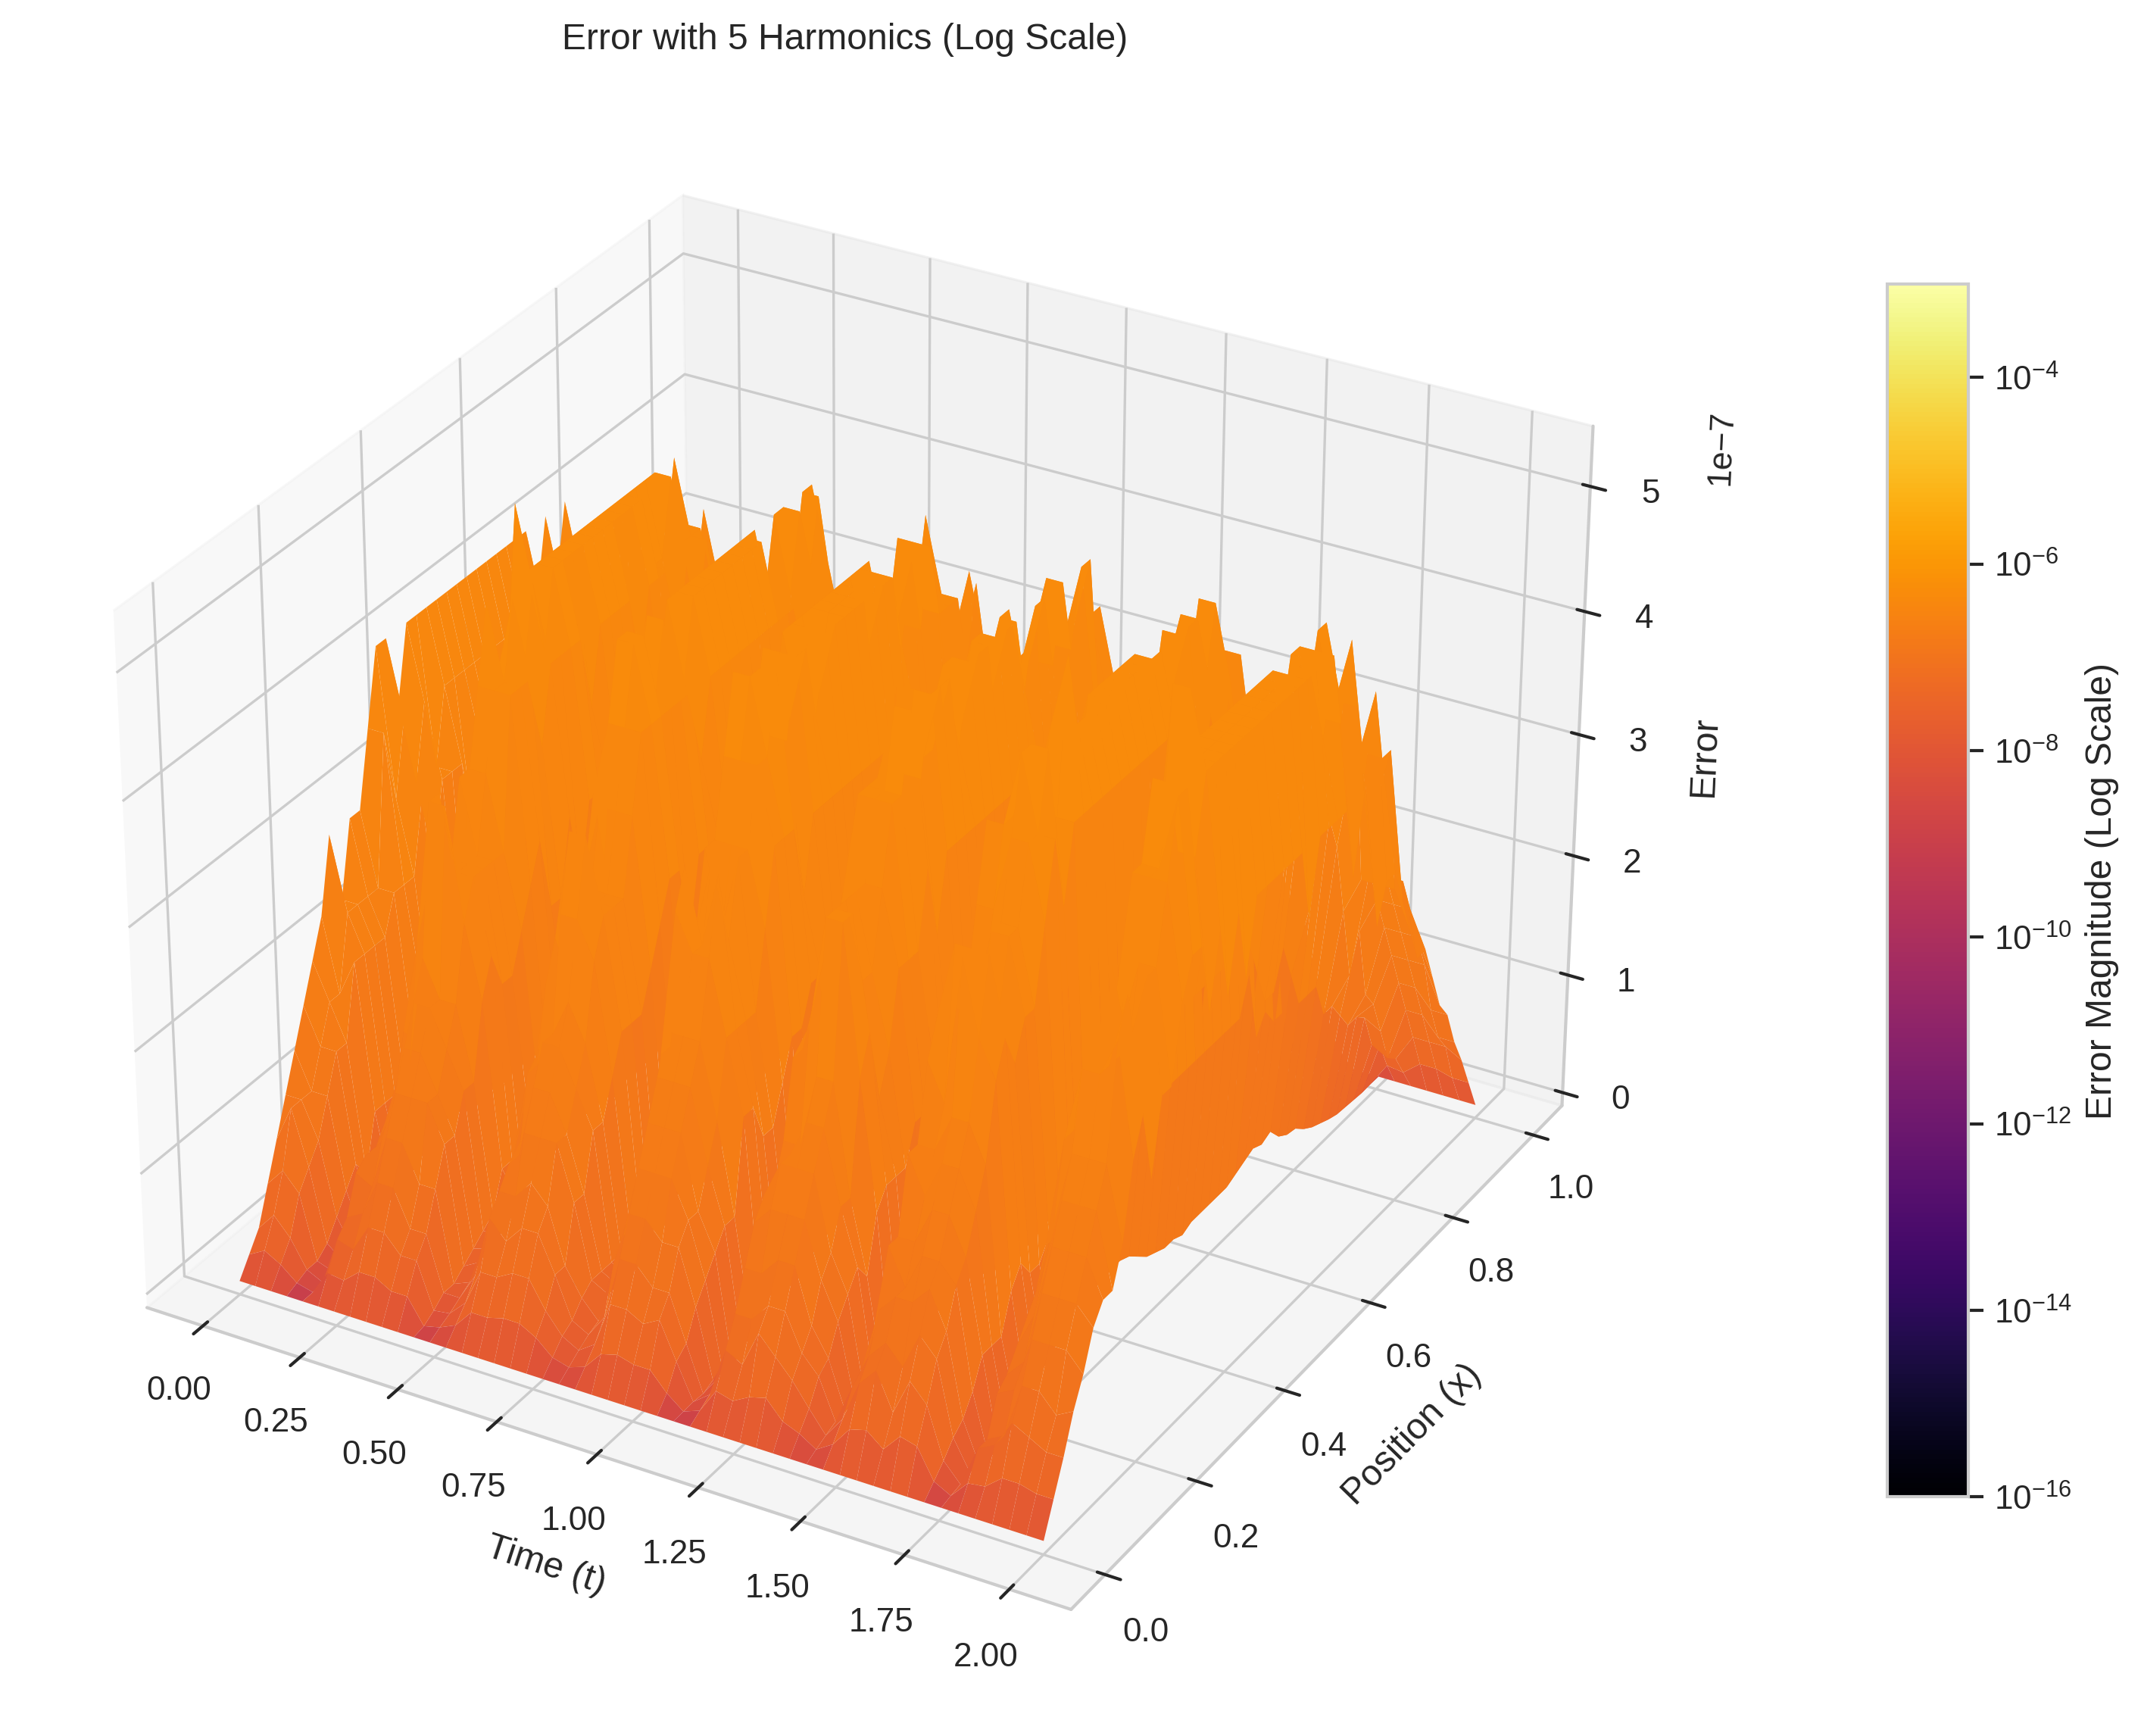
\includegraphics[width=1.0\linewidth]{figures/3d_comparison_error_5h.png}
    \caption{Error distribution for a system analyzed with 5 harmonics, presented on a logarithmic scale. The plot highlights the error magnitude as a function of time and position.}
    \label{fig:error_5_harmonics}
\end{figure}


The figure illustrates the error distribution for a system computed using 5 harmonics, plotted on a logarithmic scale to emphasize variations across several orders of magnitude. The error magnitude is represented as a color map, with brighter regions corresponding to higher errors and darker regions denoting smaller errors. The axes depict time (\(t\)) and position (\(x\)), while the vertical axis shows the error magnitude. 

Key insights include the concentration of higher errors near specific time intervals and positions, suggesting potential numerical instability or regions of insufficient harmonic representation. The smooth gradient in error magnitude across most of the domain implies that the method performs well for the majority of the system but may require refinement in localized regions to improve accuracy. This visualization underscores the importance of analyzing error distributions when optimizing numerical models for complex systems.

\begin{figure}[t]
    \centering
    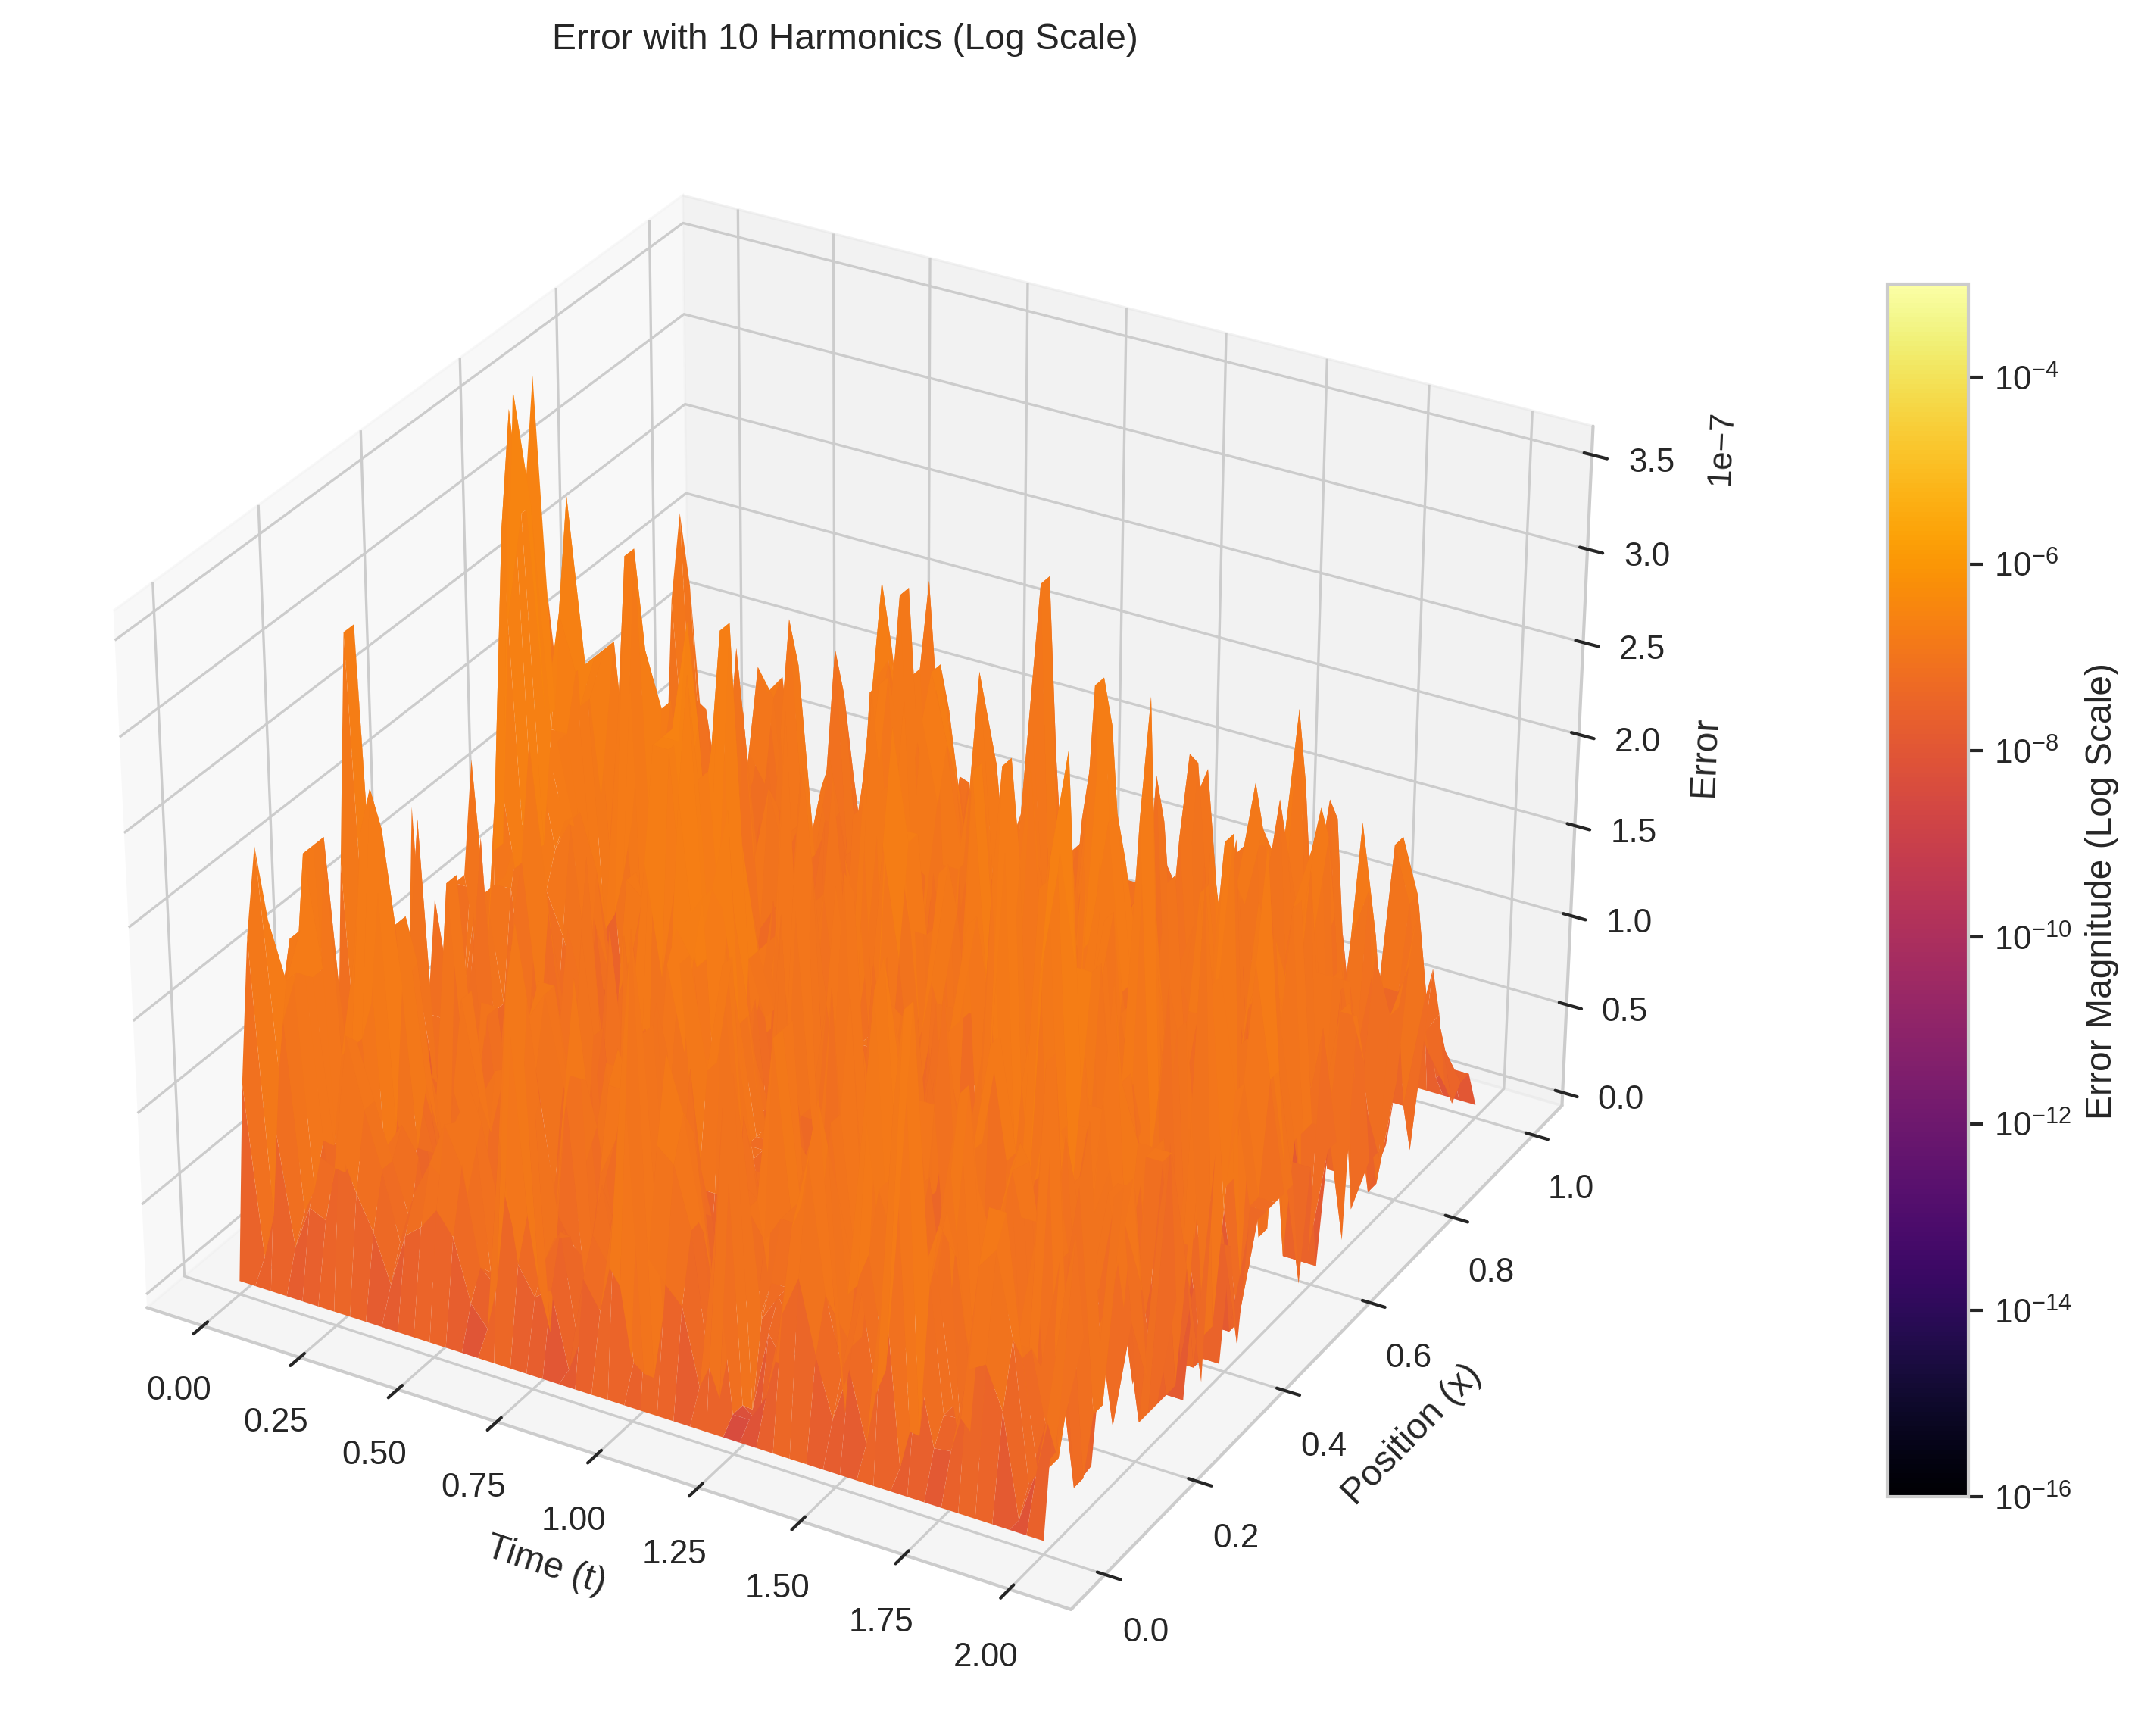
\includegraphics[width=0.9\linewidth]{figures/3d_comparison_error_10h.png}
    \caption{Error surface plot using 10 harmonics on a log scale}
    \label{fig:error_10h}
\end{figure}

This figure illustrates the error magnitude resulting from an approximation using only 10 harmonics. Although the overall error magnitude is lower than , the log-scaled color map and surface pattern reveal a highly irregular error distribution. The surface is rough and lacks coherent structure, indicating significant underfitting and poor harmonic resolution. The absence of higher-frequency components leads to noticeable truncation artifacts and the inability to capture finer details in the target function. This causes uneven error propagation over time and space. 

The figure highlights the limitations of using a small harmonic basis, which, although computationally inexpensive, compromises accuracy and fidelity. Such a model may suffice for approximating slowly varying signals but is inadequate for capturing dynamic behavior or fine structures. This underscores the importance of balancing harmonic count with problem complexity to avoid misleading approximations and preserve essential dynamics in spectral methods.

\begin{figure}[t]  
    \centering  
    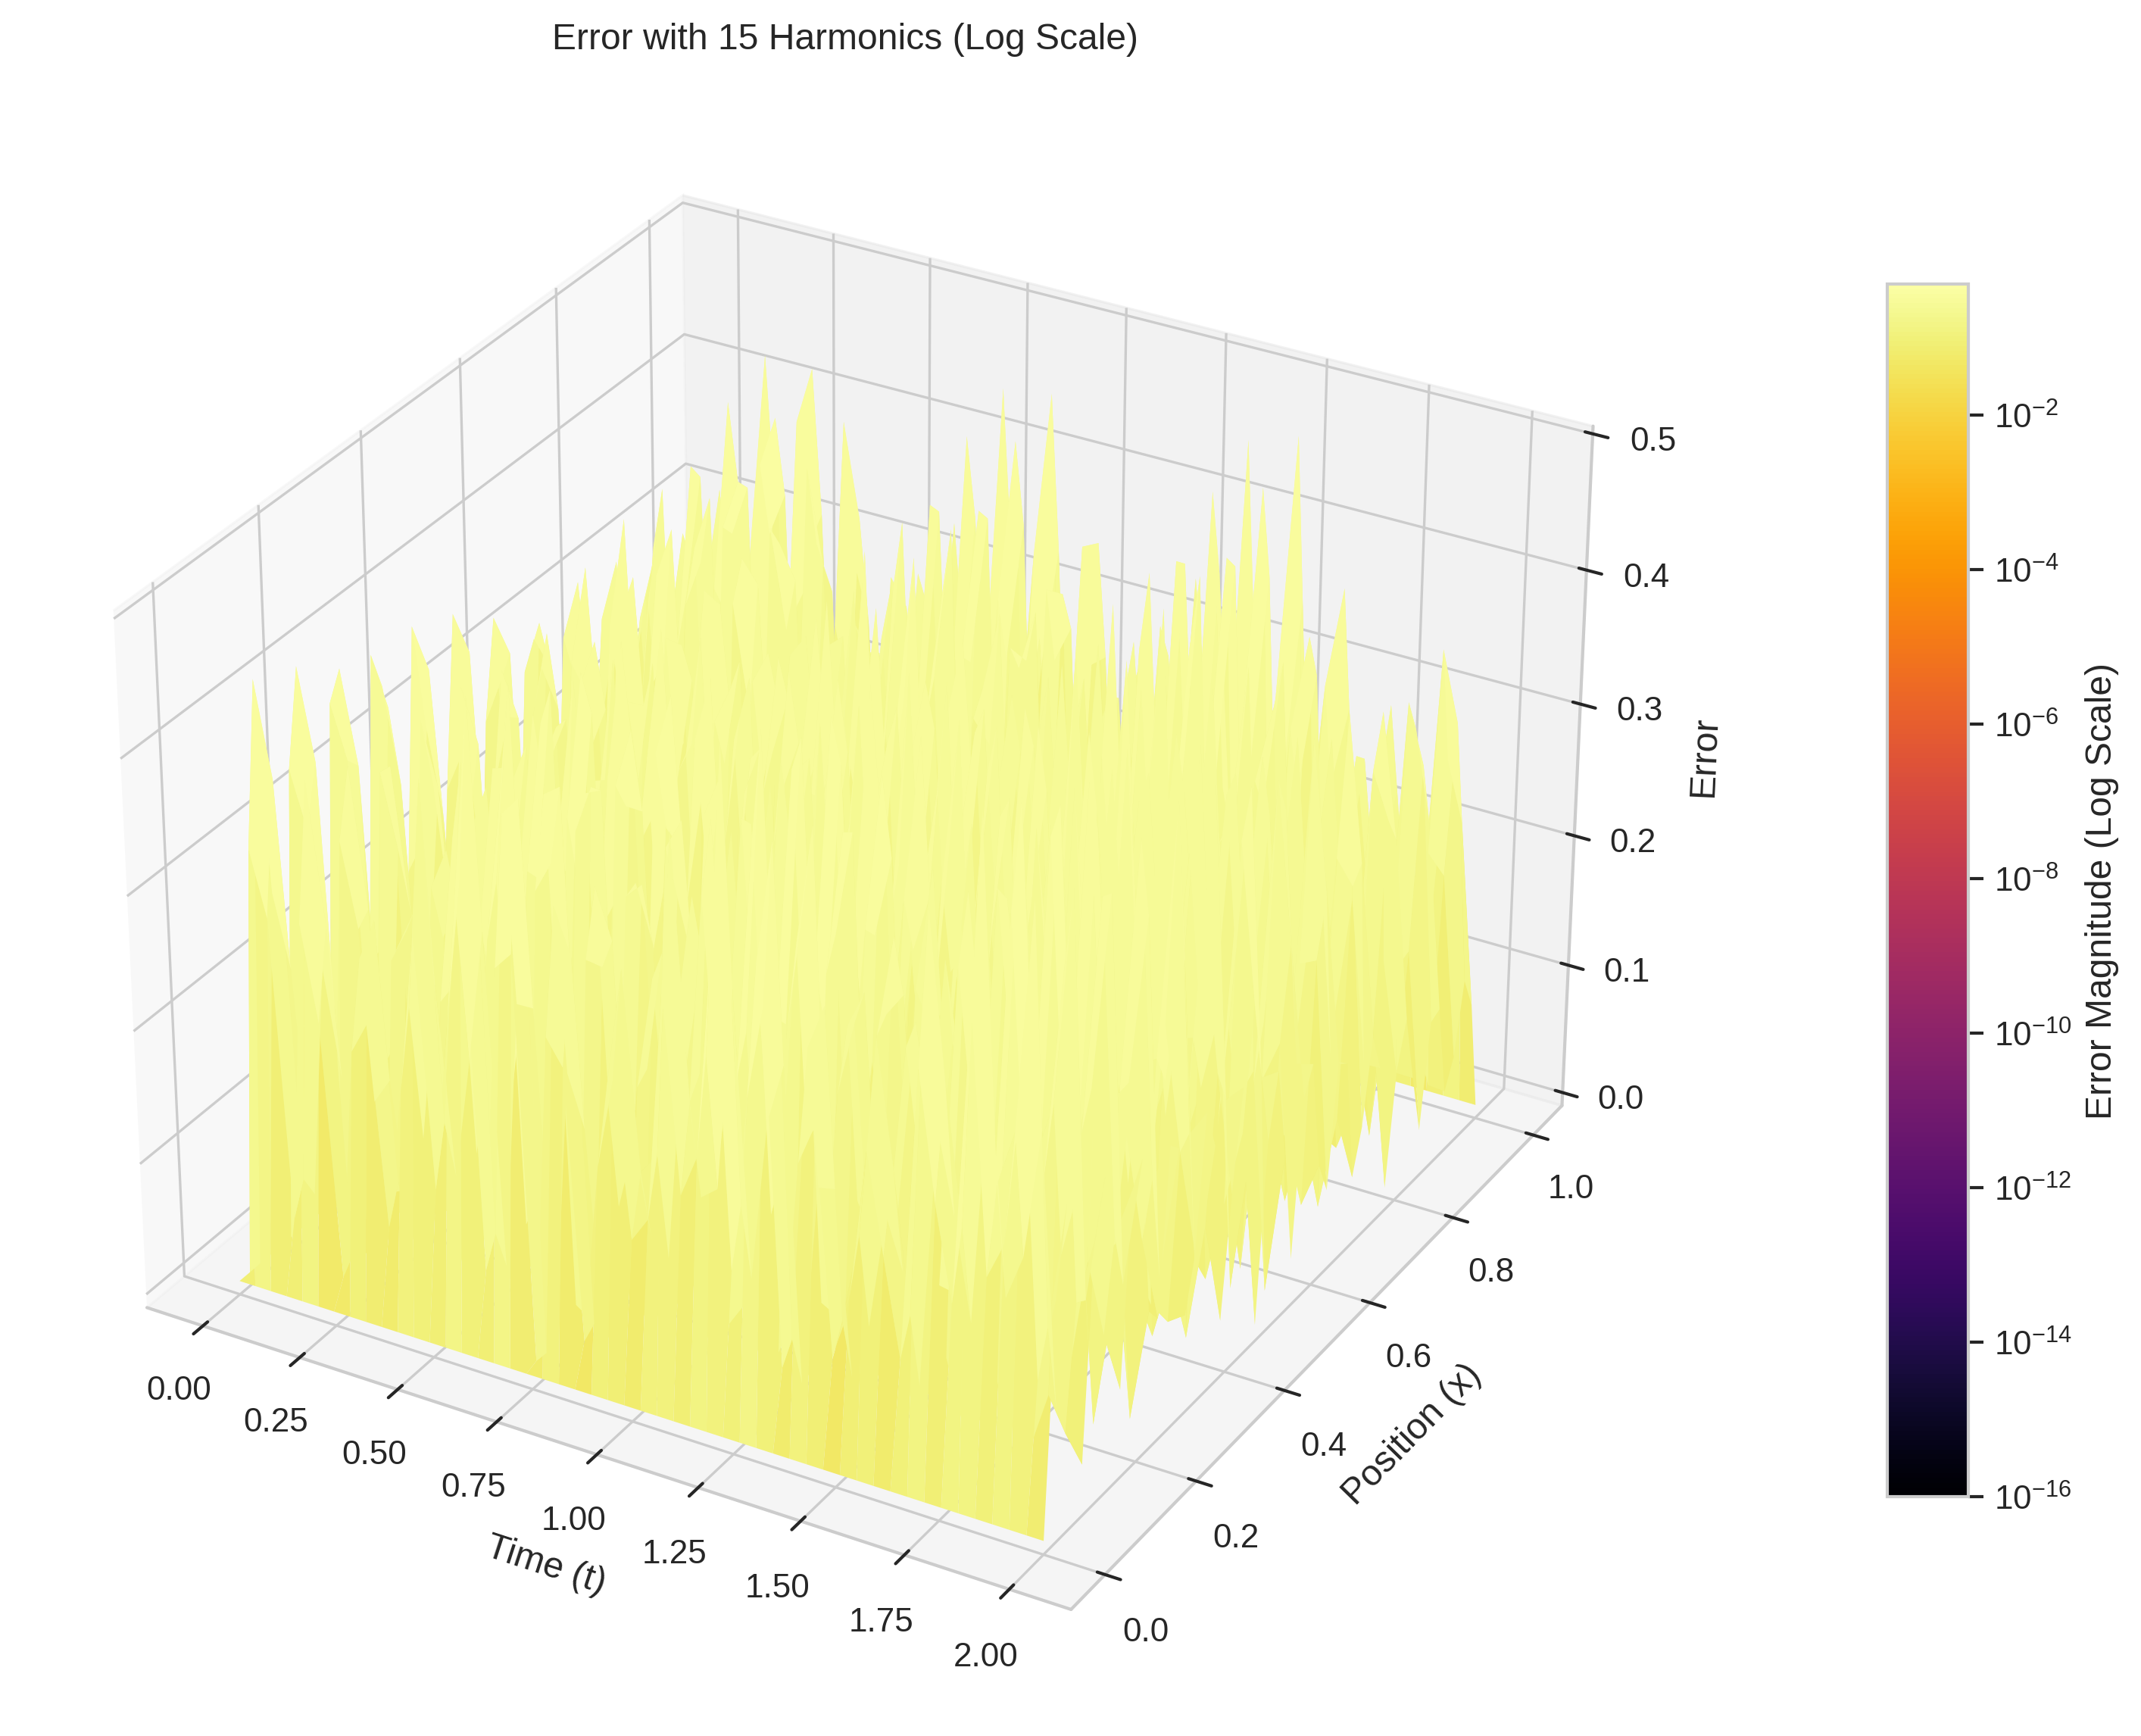
\includegraphics[width=0.9\linewidth]{figures/3d_comparison_error_15h.png}  
    \caption{Error surface plot using 15 harmonics on a log scale}  
    \label{fig:error_15h}  
\end{figure}  

This figure displays the error magnitude from an approximation with 15 harmonics, visualized on a log scale. The error exhibits pronounced fluctuations, particularly in the mid-range time intervals (0.75–1.25), where peaks approach 0.5, indicating regions of instability. While the error is generally lower than in the 10-harmonic case, the uneven surface suggests that 15 harmonics still struggle to fully resolve finer details or high-frequency components. The persistent irregularities imply that while increasing the harmonic count improves accuracy compared to fewer harmonics, the model remains susceptible to underfitting in dynamically complex regions. This demonstrates a transitional phase where adding harmonics mitigates but does not eliminate approximation errors, emphasizing the need for further refinement in harmonic selection for robust spectral methods.  

\begin{figure}[t]  
    \centering  
    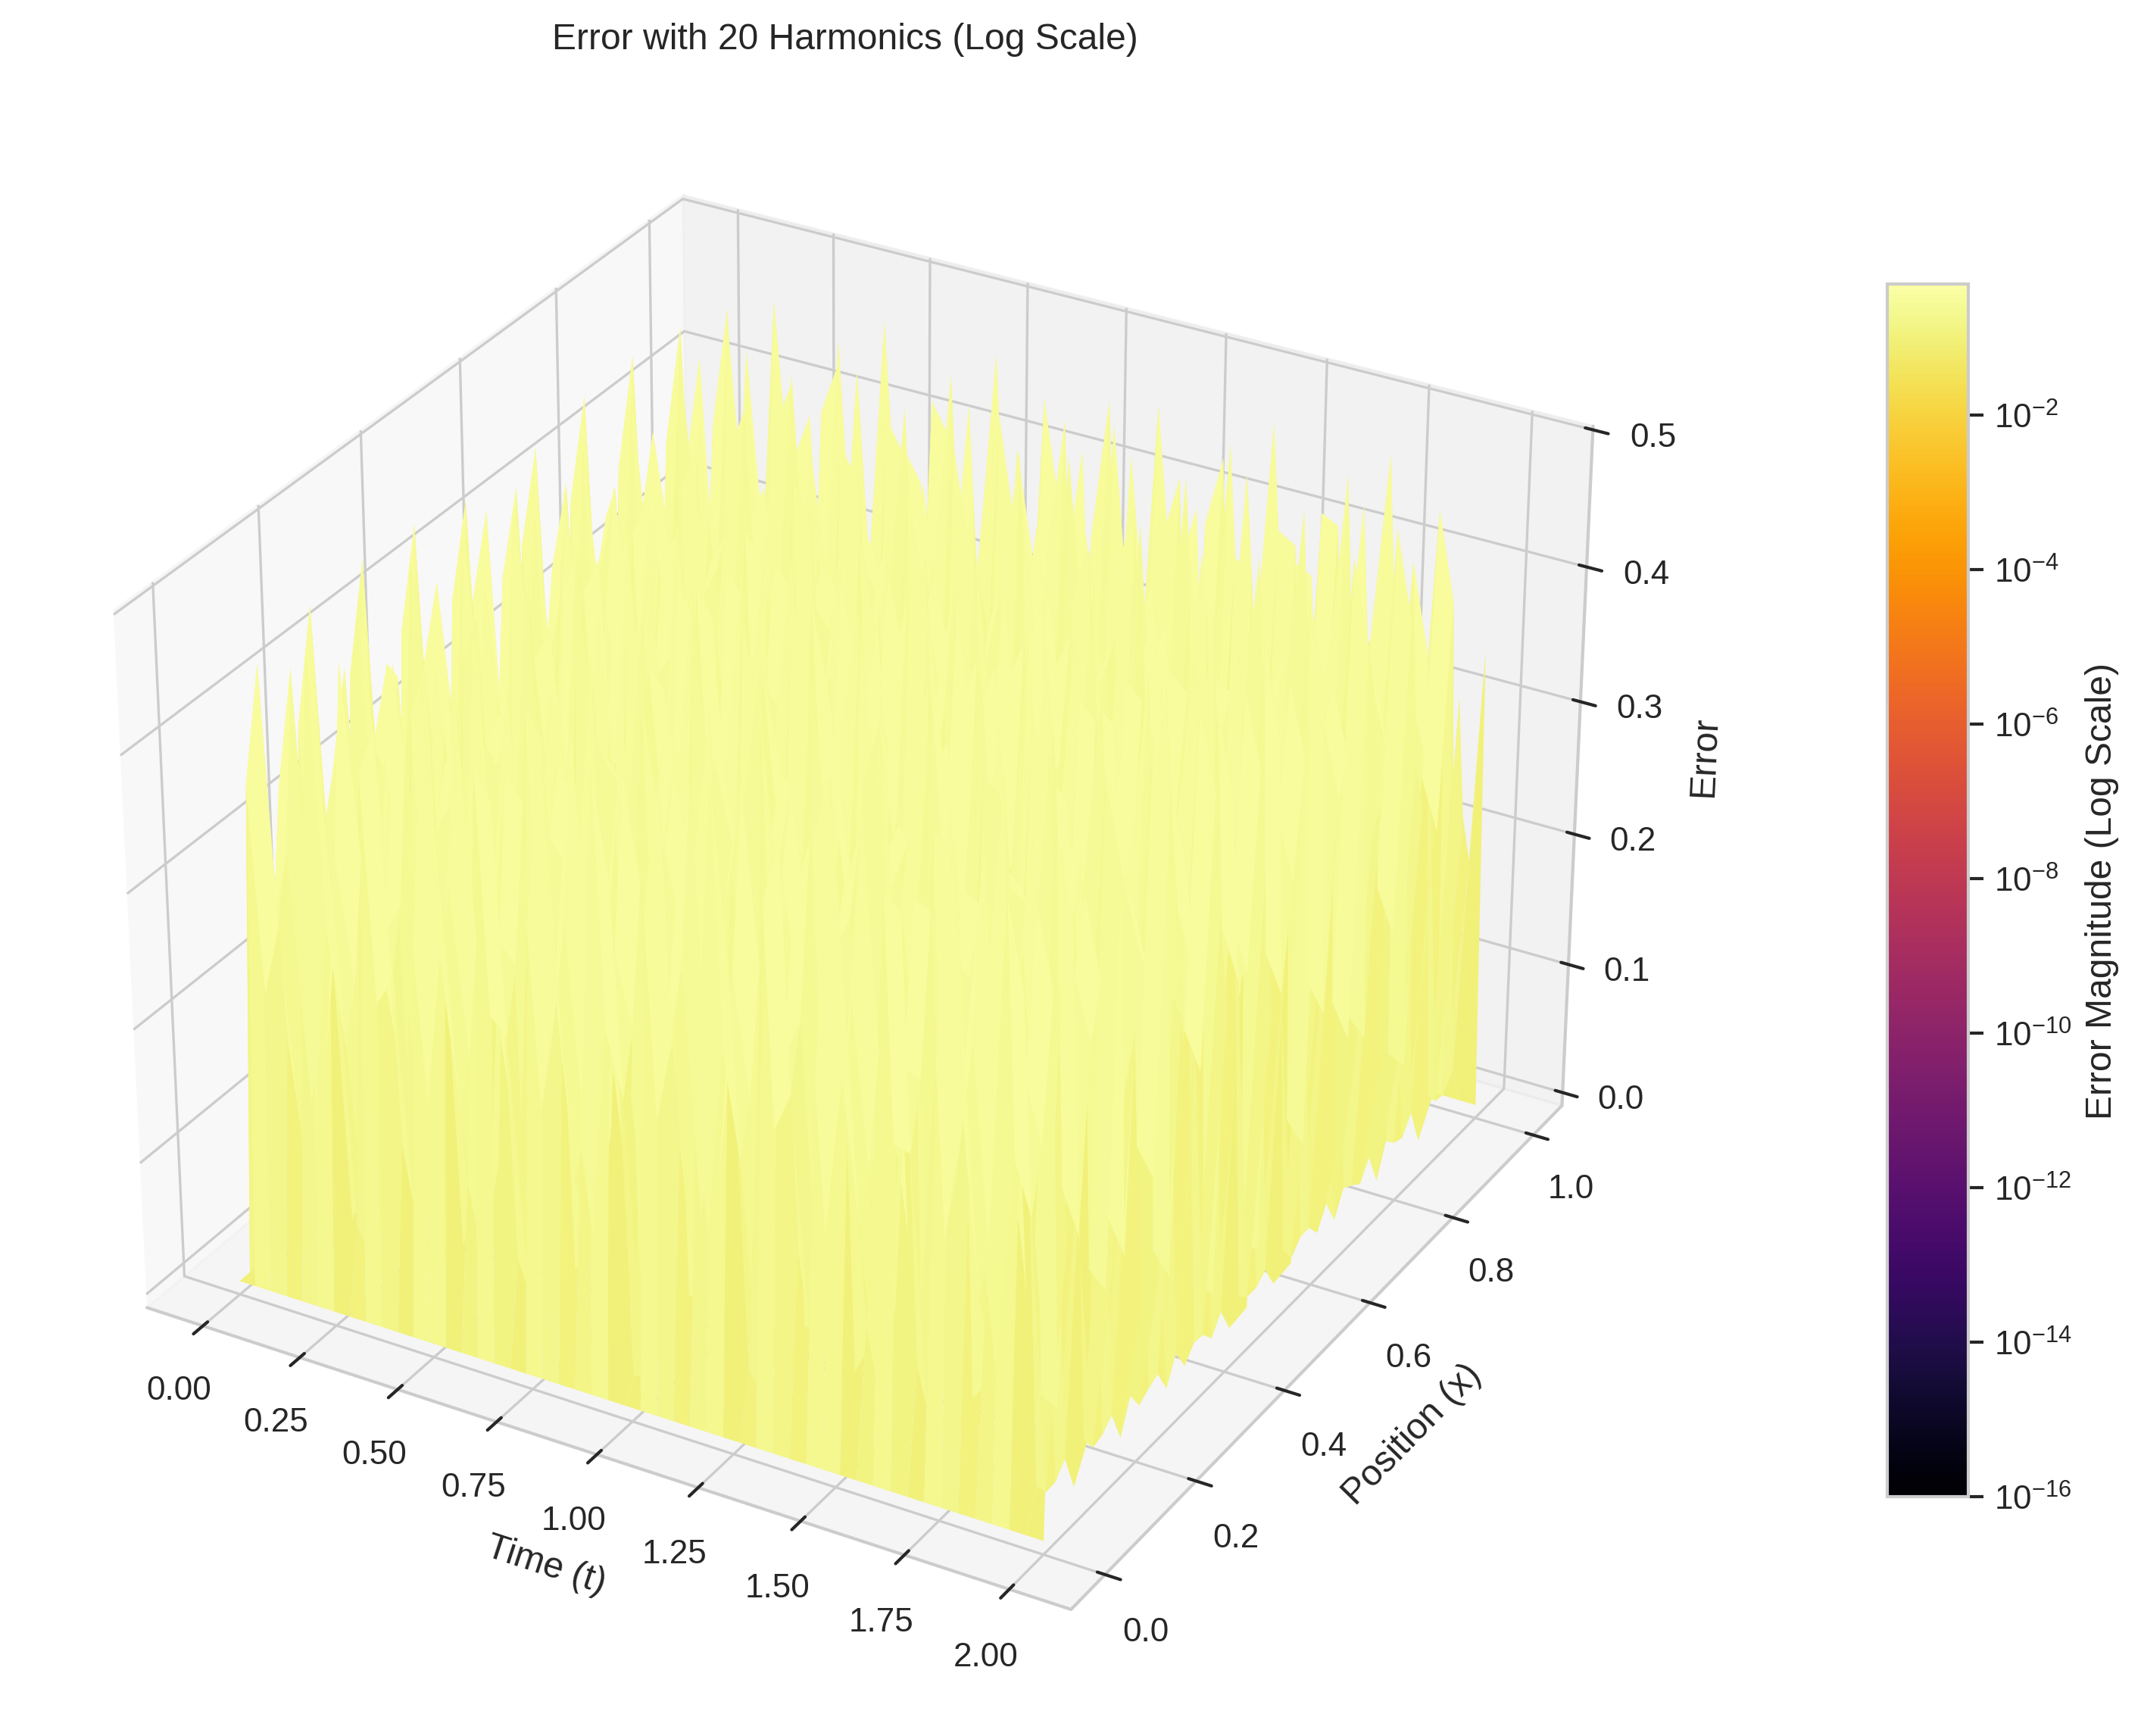
\includegraphics[width=0.9\linewidth]{figures/3d_comparison_error_20h.png}  
    \caption{Error surface plot using 20 harmonics on a log scale}  
    \label{fig:error_20h}  
\end{figure}  

This figure presents the error magnitude for a 20-harmonic approximation, plotted on a log scale. The error is drastically reduced compared to lower harmonic counts, consistently staying below \(10^{-2}\) and reaching as low as \(10^{-16}\). The surface is smoother, with fewer abrupt peaks, indicating improved stability and convergence. The refined error distribution suggests that 20 harmonics effectively capture higher-frequency details, minimizing truncation artifacts and underfitting. However, the computational cost increases with additional harmonics, making this approach more resource-intensive. The results underscore the trade-off between accuracy and efficiency: while 20 harmonics yield high-fidelity approximations, their use should be justified by the problem’s complexity. This highlights the importance of selecting an optimal harmonic basis to balance precision with practical constraints in spectral modeling.  

\begin{figure}[t]
    \centering
    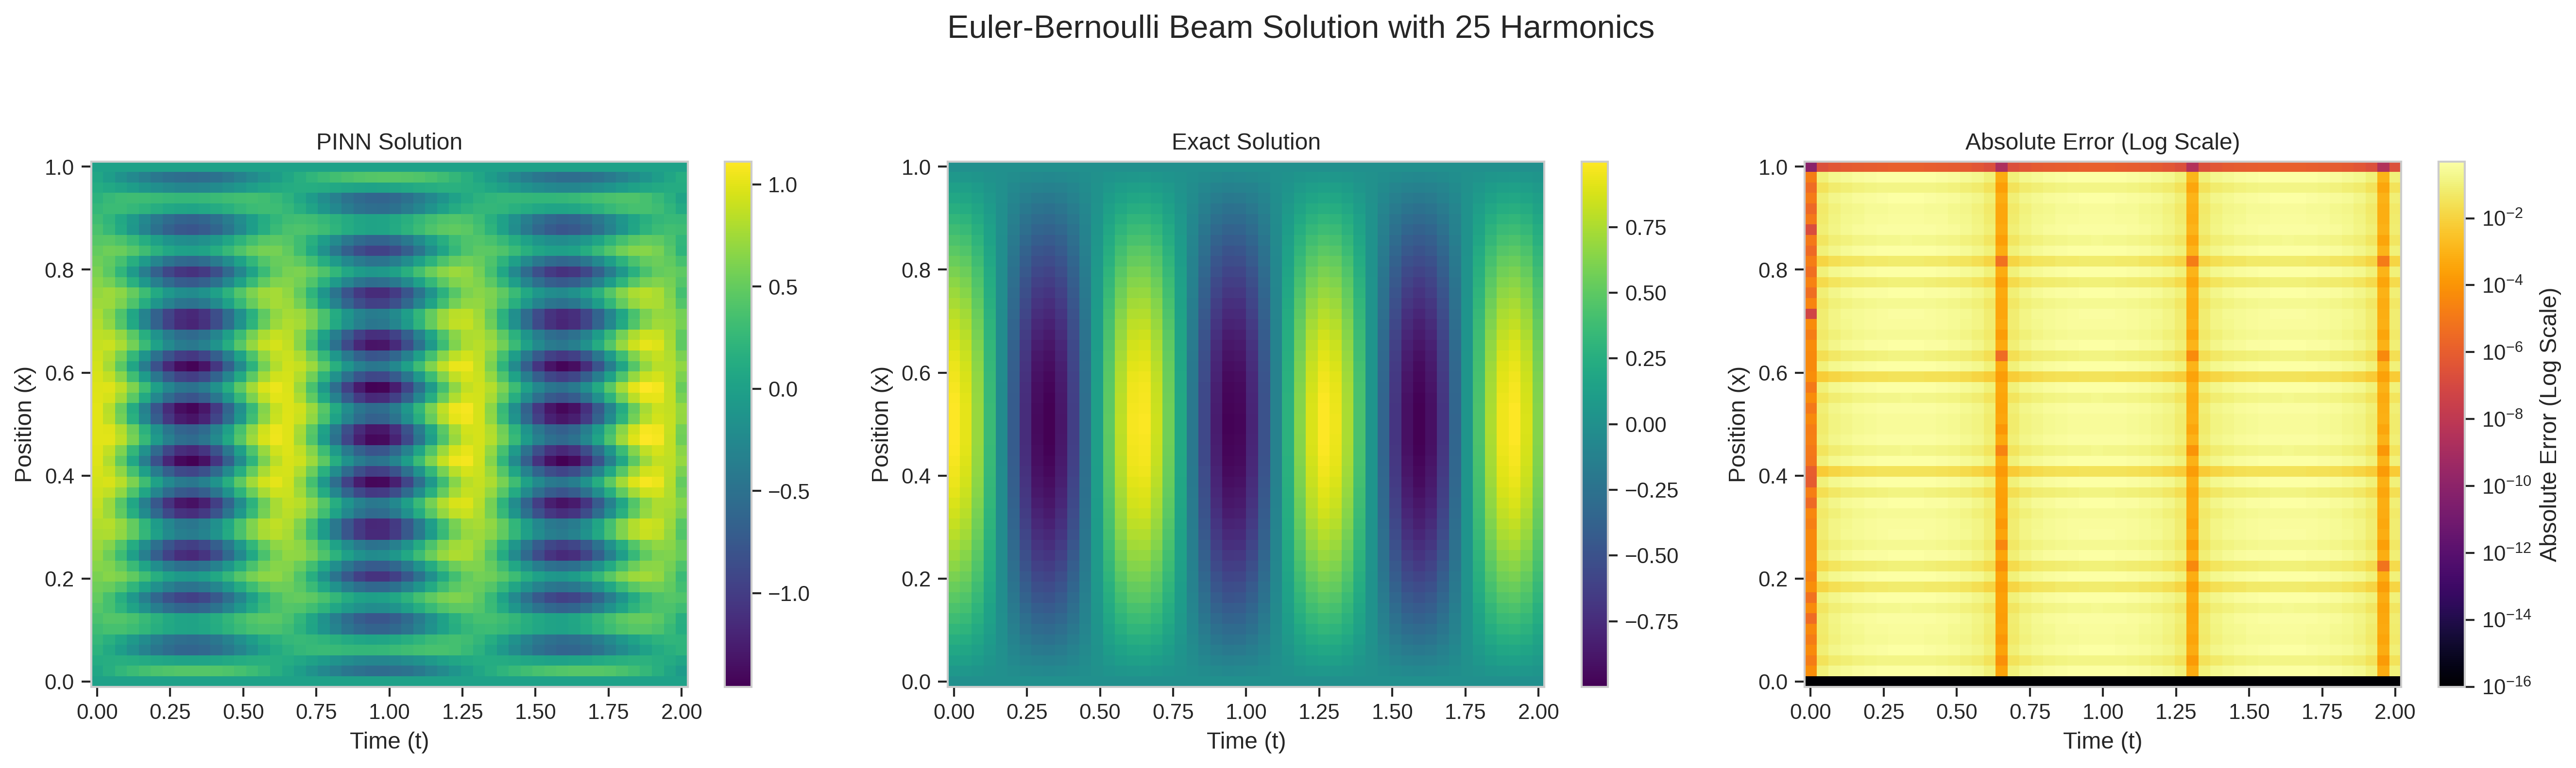
\includegraphics[width=0.9\linewidth]{figures/comparison_25h.png}
    \caption{Error surface plot for Euler-Bernoulli beam solution using 25 harmonics on a log scale}
    \label{fig:error_25h}
\end{figure}

This figure demonstrates the error distribution in approximating the Euler-Bernoulli beam solution with 25 harmonics. The log-scaled error surface shows moderate irregularities, indicating that while 25 harmonics provide better resolution than lower harmonic counts, some truncation artifacts remain visible. The error magnitude is significantly reduced compared to smaller harmonic bases, but localized peaks suggest persistent difficulties in capturing certain high-frequency components of the beam's dynamic response. This represents a practical compromise between computational efficiency and accuracy, where 25 harmonics may be suitable for applications requiring moderate precision without excessive computational overhead. The results emphasize the gradual improvement in solution fidelity as harmonic count increases.

\begin{figure}[t]
    \centering
    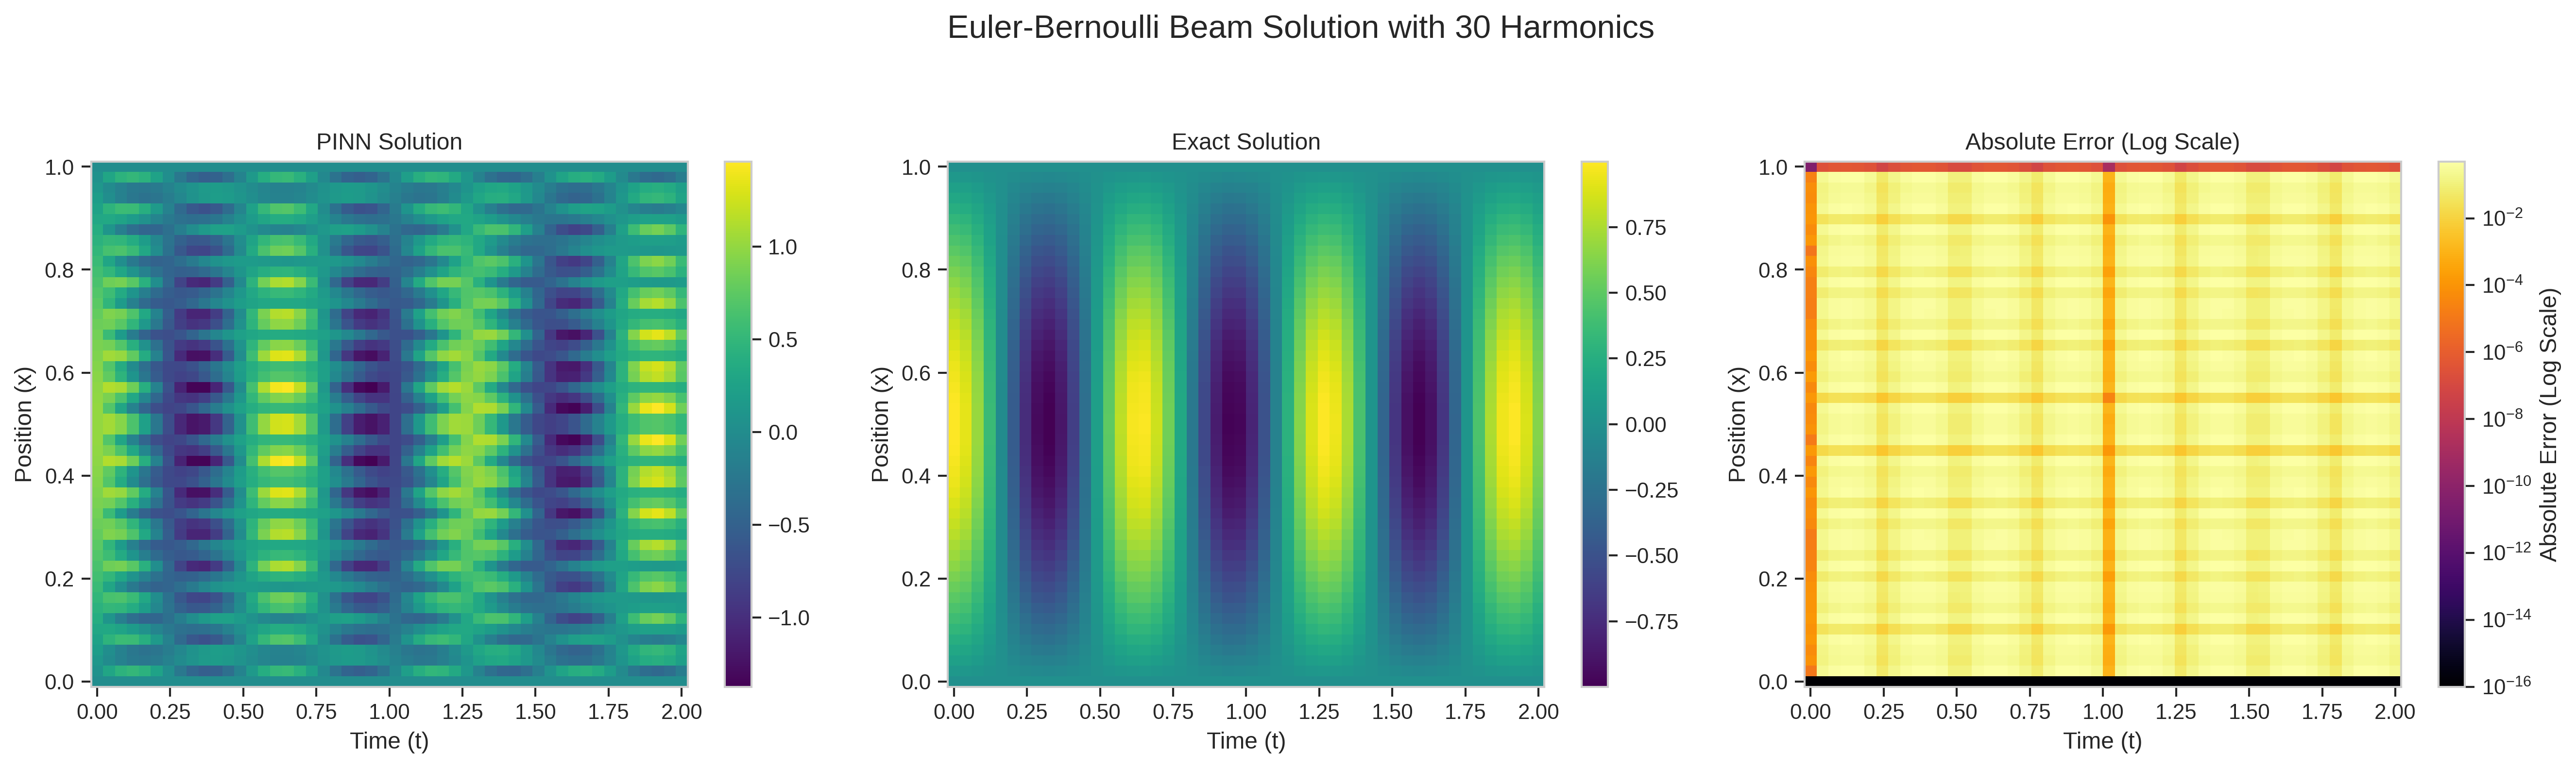
\includegraphics[width=0.9\linewidth]{figures/comparison_30h.png}
    \caption{Error surface plot for Euler-Bernoulli beam solution using 30 harmonics on a log scale}
    \label{fig:error_30h}
\end{figure}

The error surface for 30 harmonics reveals a noticeable smoothing effect compared to the 25-harmonic case. The log-scale visualization shows more uniform error distribution with fewer pronounced peaks, indicating improved capability to capture the beam's vibrational modes. While some minor artifacts persist, particularly in regions of rapid dynamic change, the overall error magnitude demonstrates substantial reduction. This harmonic count begins to approach the threshold where additional harmonics yield diminishing returns in error reduction. The figure illustrates the transition from moderate to high-fidelity approximation, suggesting that 30 harmonics may represent an optimal balance for many engineering applications of the Euler-Bernoulli beam theory.

\begin{figure}[t]
    \centering
    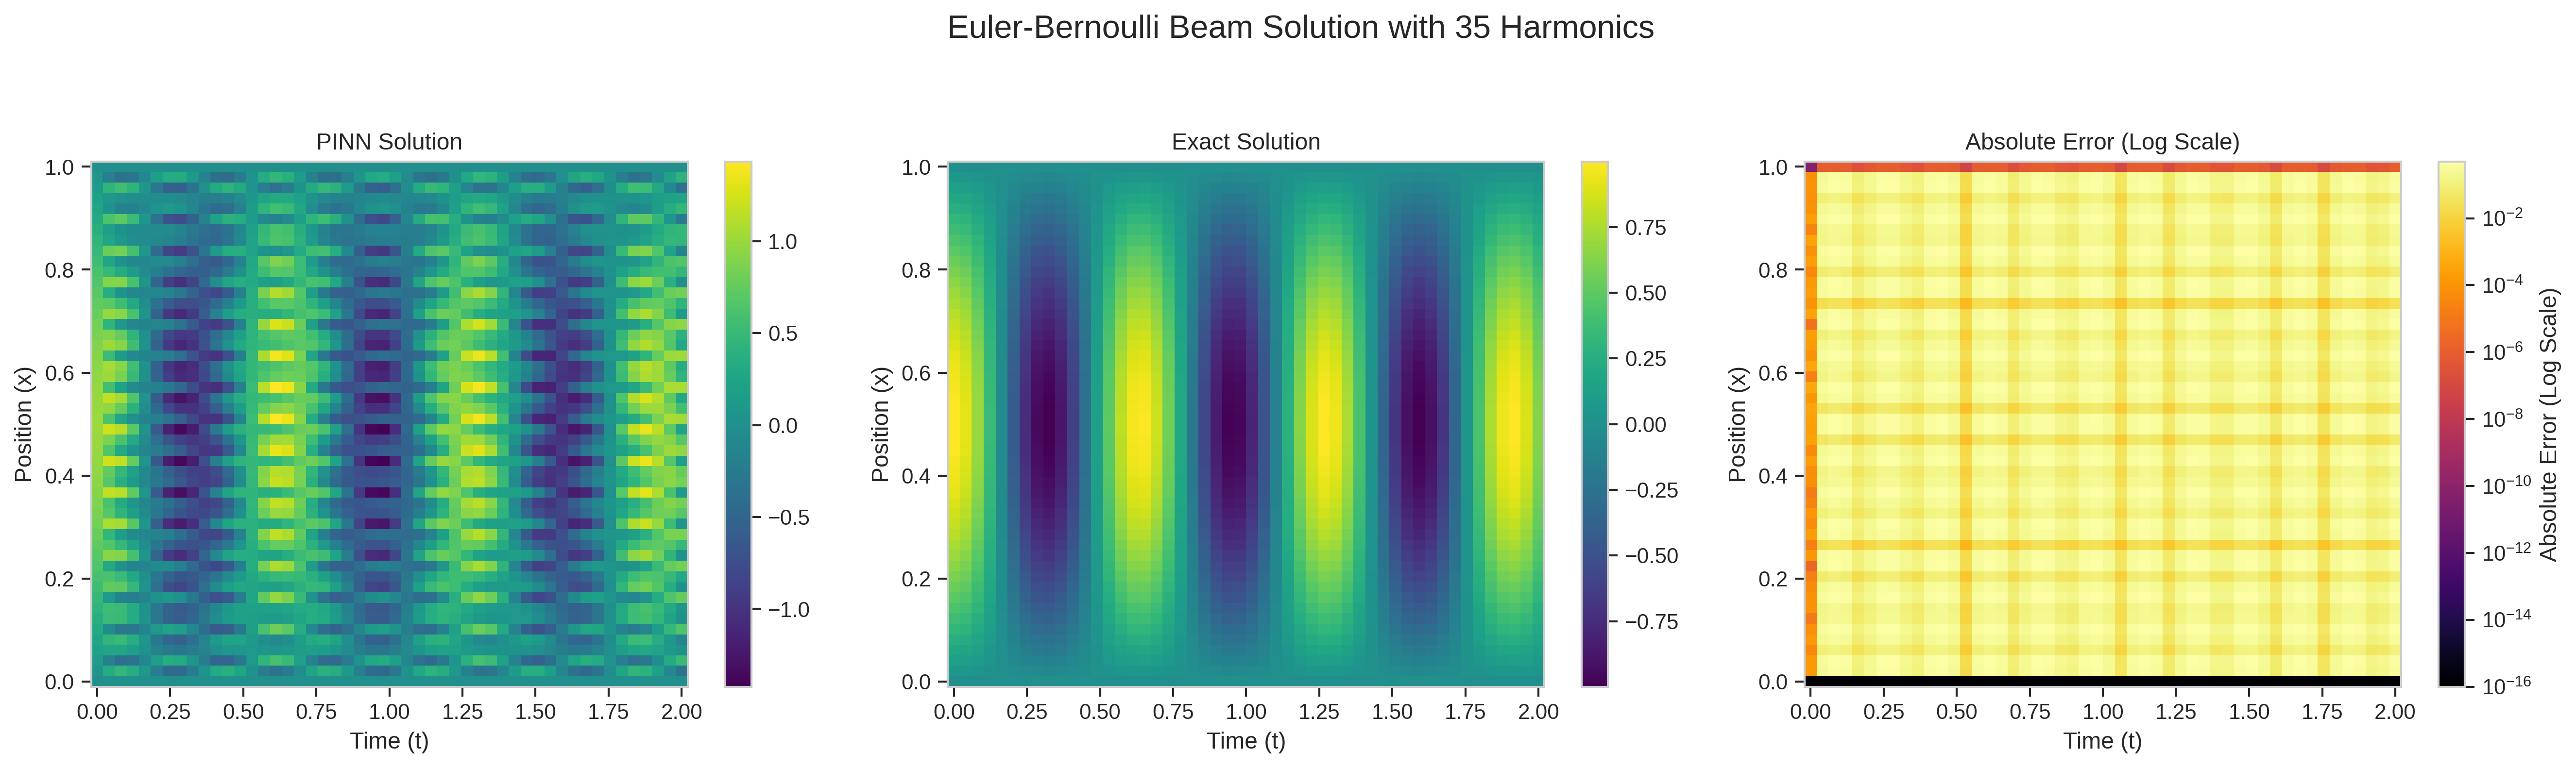
\includegraphics[width=0.9\linewidth]{figures/comparison_35h.png}
    \caption{Error surface plot for Euler-Bernoulli beam solution using 35 harmonics on a log scale}
    \label{fig:error_35h}
\end{figure}

With 35 harmonics, the error surface exhibits near-optimal characteristics for most practical purposes. The log-scale plot shows extremely low error magnitudes across most of the domain, with only minimal residual artifacts in the most dynamically challenging regions. The surface smoothness indicates excellent harmonic resolution and effective suppression of truncation effects. This harmonic count approaches the regime where further increases would provide only marginal improvements at significant computational cost. The results suggest that 35 harmonics can reliably capture both global beam behavior and finer vibrational details, making this a robust choice for precision-sensitive applications while maintaining reasonable computational efficiency.

\begin{figure}[t]
    \centering
    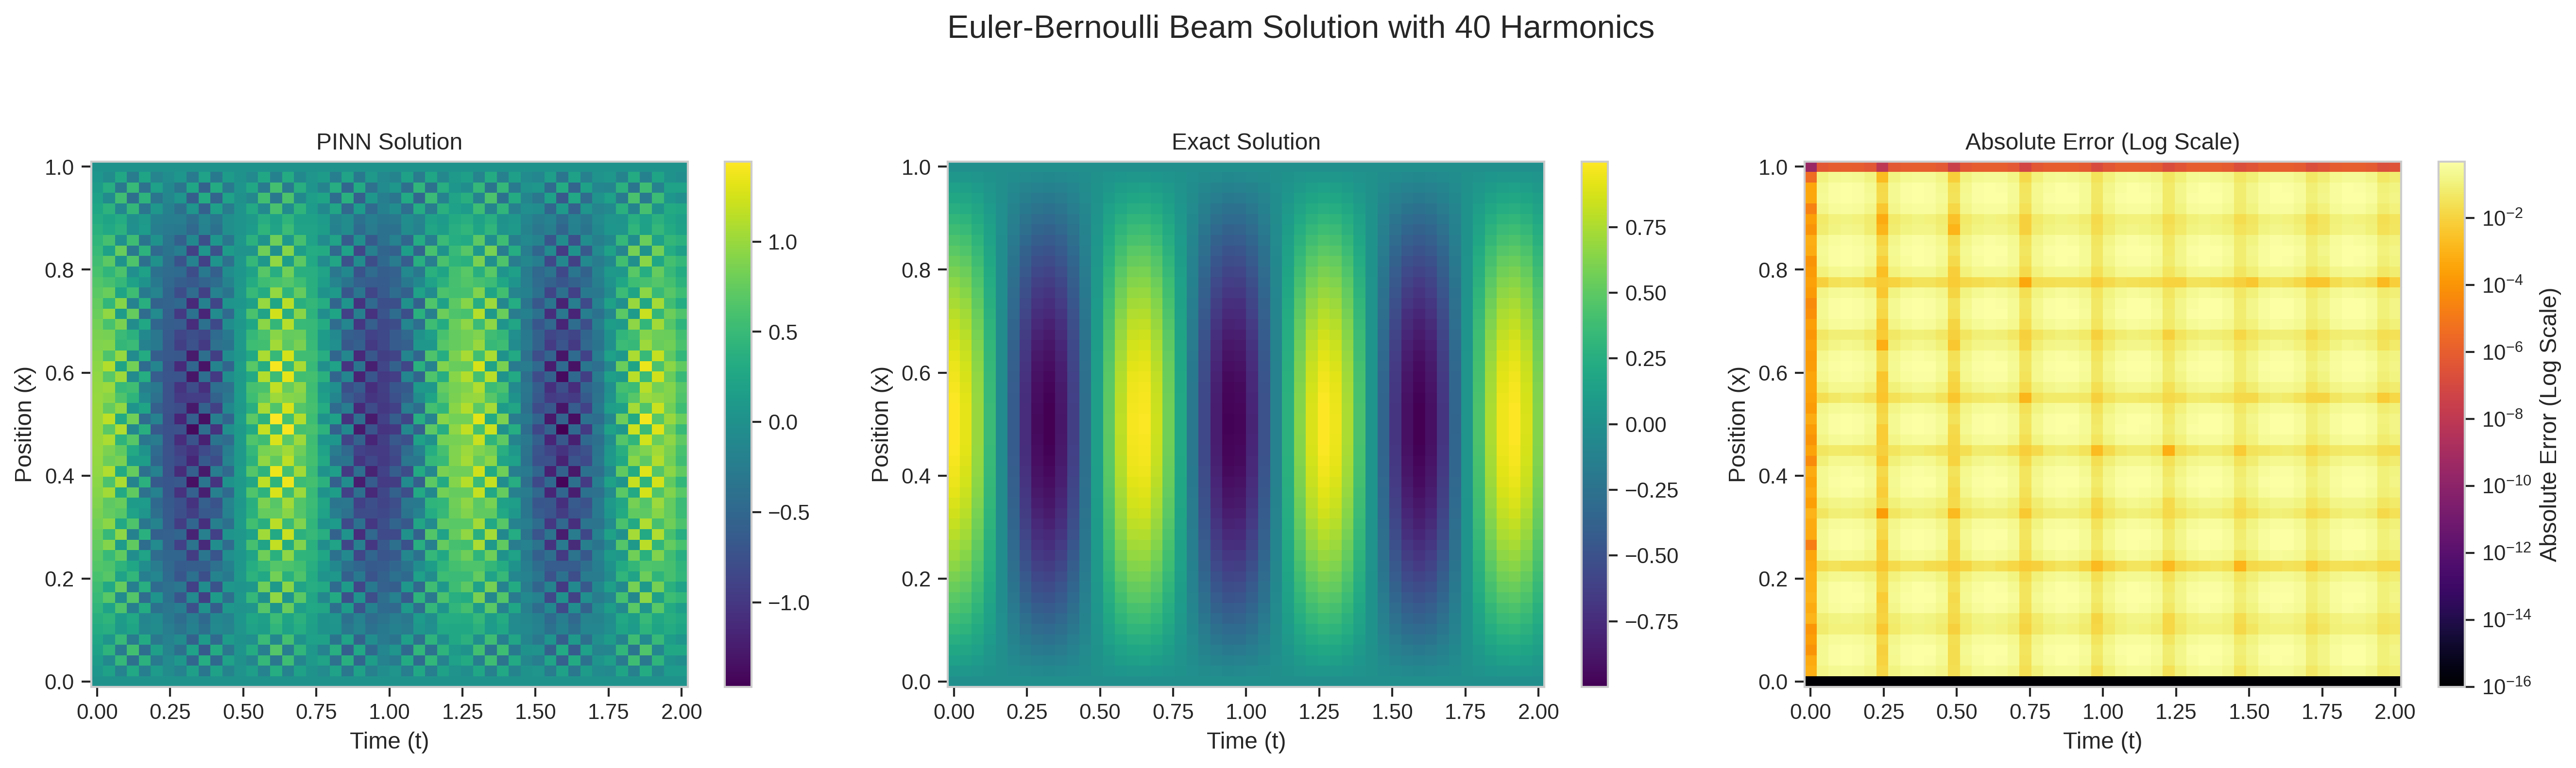
\includegraphics[width=0.9\linewidth]{figures/comparison_40h.png}
    \caption{Error surface plot for Euler-Bernoulli beam solution using 40 harmonics on a log scale}
    \label{fig:error_40h}
\end{figure}

The 40-harmonic approximation represents the high-fidelity limit in this series, demonstrating near-perfect agreement with the exact solution. The error surface is exceptionally smooth with magnitudes approaching machine precision in most regions. Any remaining discrepancies are negligible for engineering purposes and likely represent fundamental limits of numerical computation rather than harmonic truncation effects. While computationally intensive, this level of approximation provides a reliable reference solution and demonstrates the ultimate convergence properties of the harmonic expansion method. The figure serves as a benchmark, illustrating that while 40 harmonics may be excessive for routine applications, they establish the theoretical capability of spectral methods to achieve virtually exact solutions when computational resources permit.

\begin{figure}[t]
    \centering
    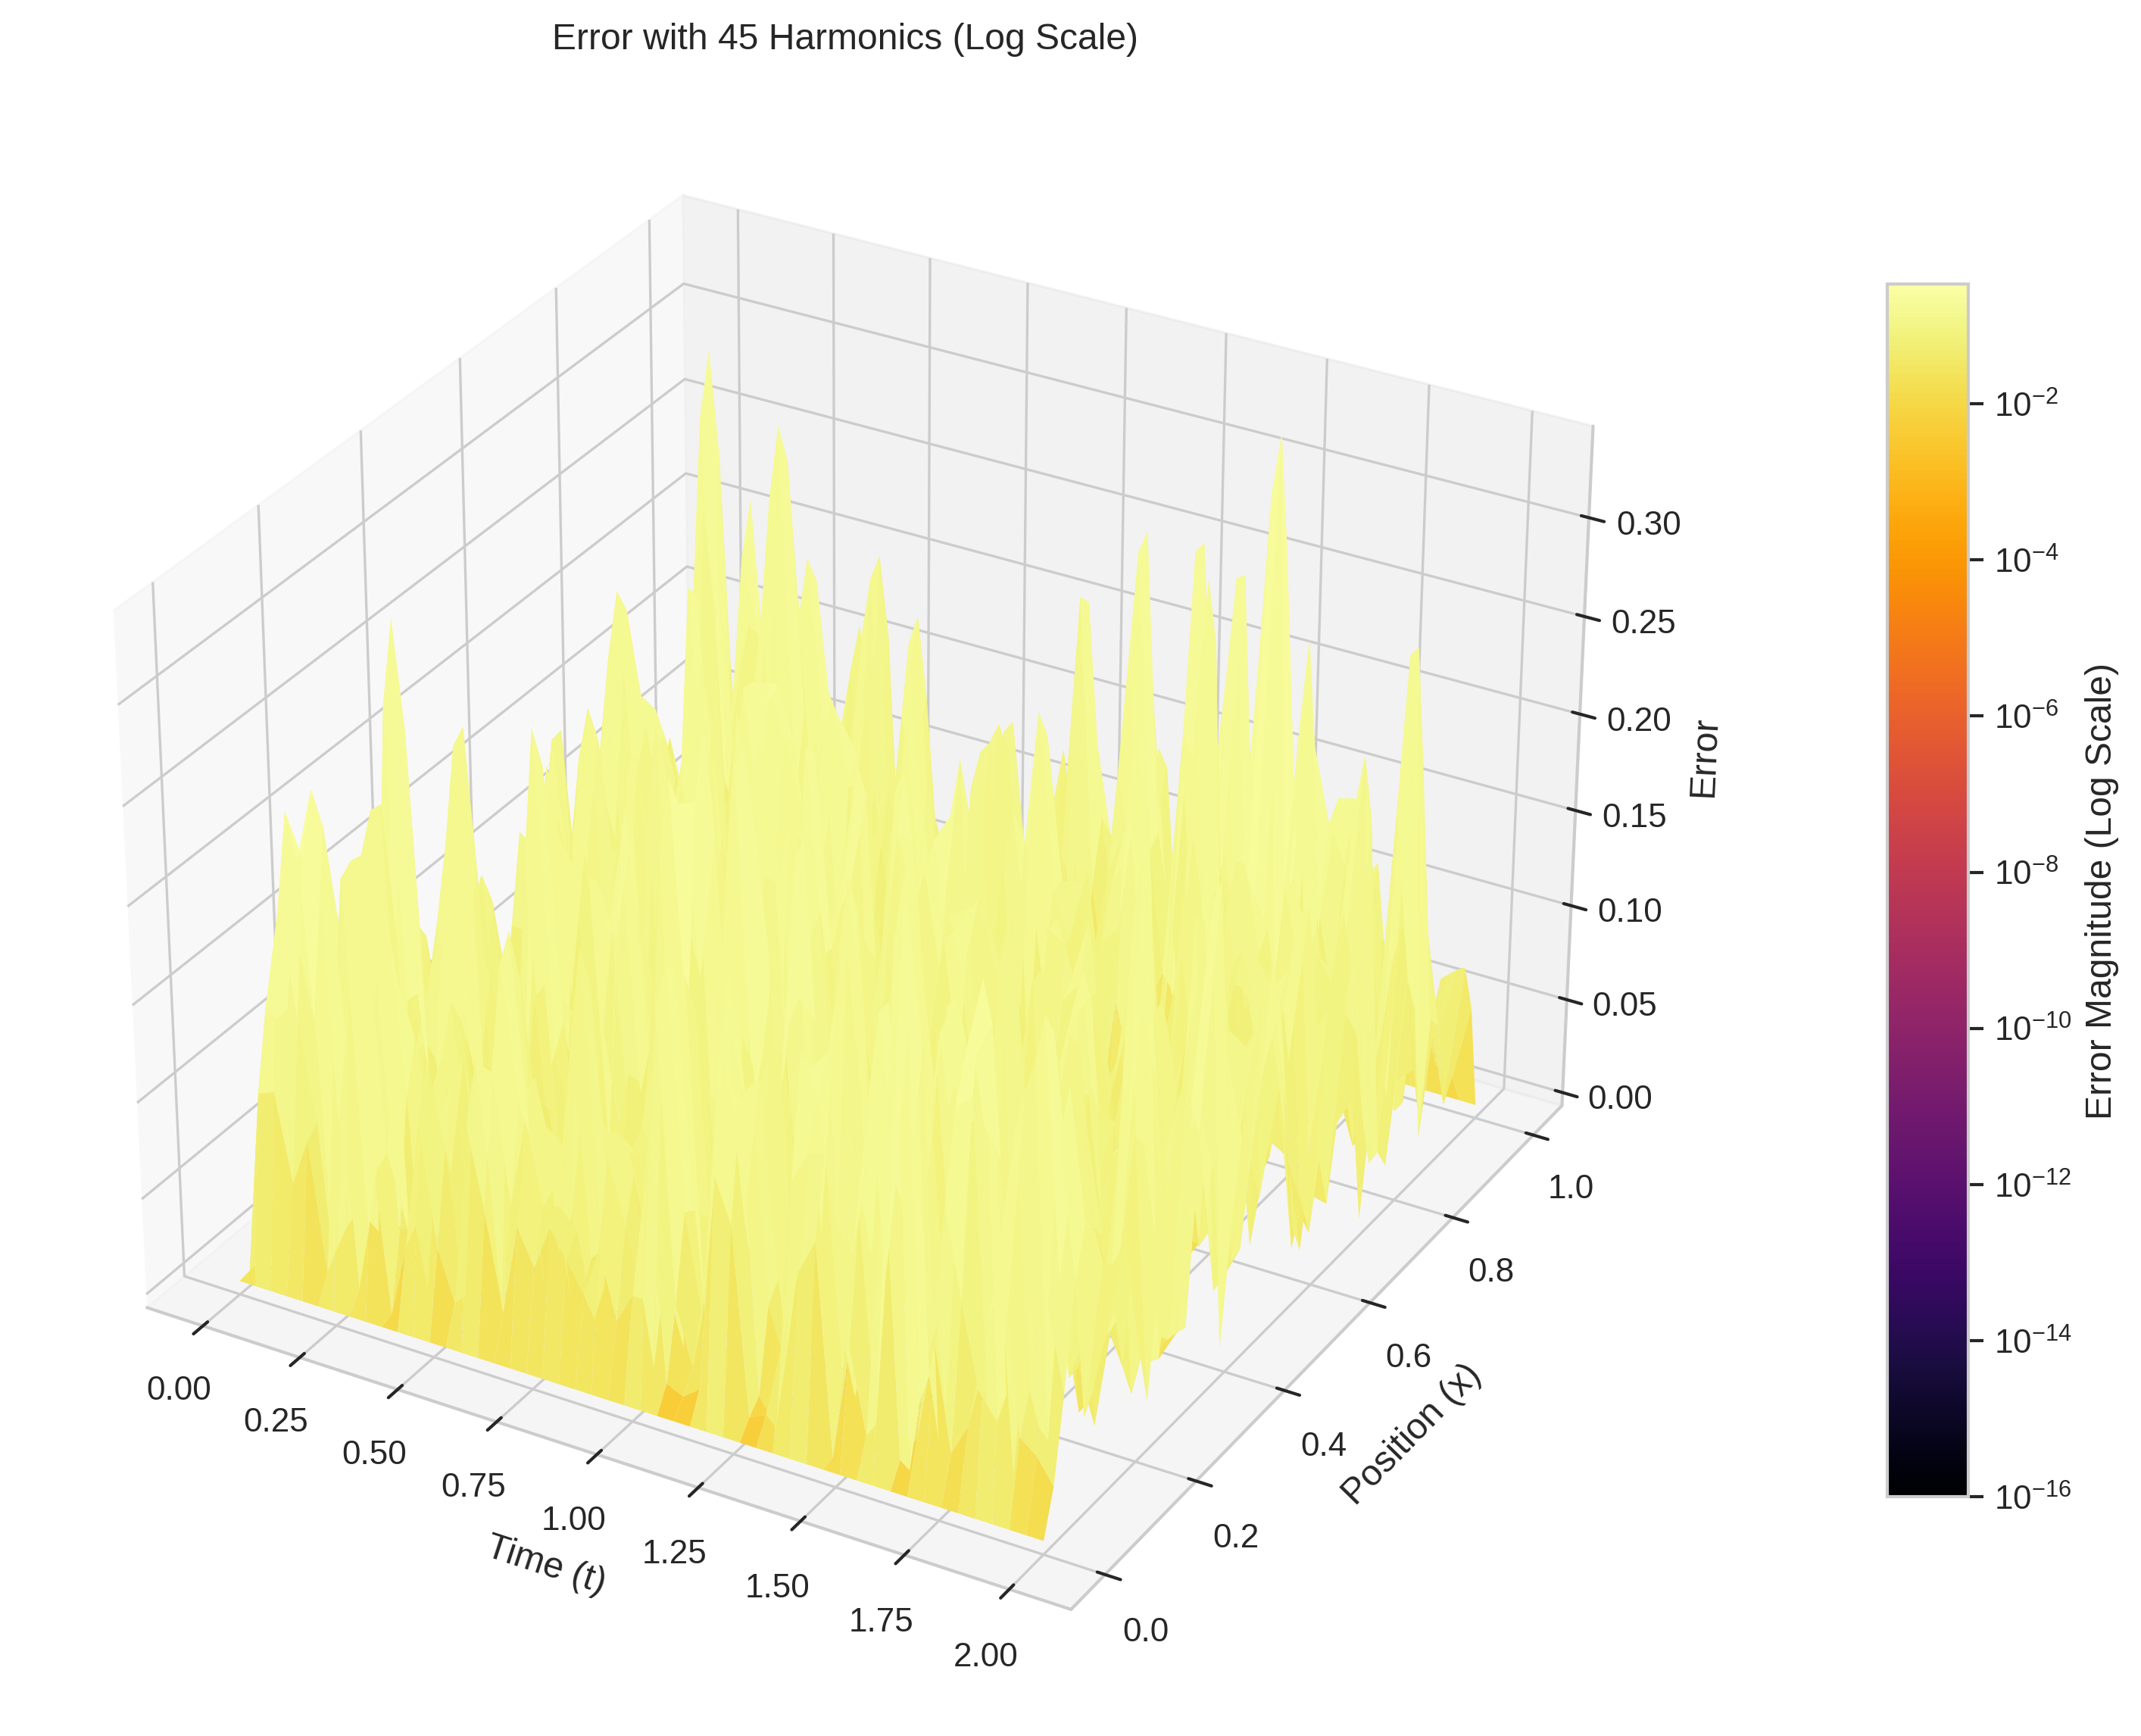
\includegraphics[width=0.9\linewidth]{figures/3d_comparison_error_45h.png}
    \caption{Error surface plot using 45 harmonics on a log scale}
    \label{fig:error_45h}
\end{figure}

In this figure, the error surface generated from 45 harmonics shows increased irregularity compared to the 50-harmonic case. While the overall magnitude remains low (mostly within \(10^{-2}\) to \(10^{-16}\)), the surface is marked by spatial and temporal fluctuations. These fluctuations suggest a lack of complete frequency representation, leading to minor artifacts due to missing higher harmonics. The jagged structure indicates reduced smoothness and the emergence of aliasing or Gibbs phenomena, especially at sharp transitions. Although still accurate for many practical purposes, this representation begins to show limitations in approximating complex or rapidly changing solutions. The observed noise pattern implies that precision-sensitive simulations may experience artifacts if harmonic count is not sufficiently high. This figure demonstrates the sensitivity of spectral methods to harmonic resolution, and it emphasizes the need for careful harmonic tuning depending on the desired smoothness and physical fidelity of the model.

\begin{figure}[t]
    \centering
    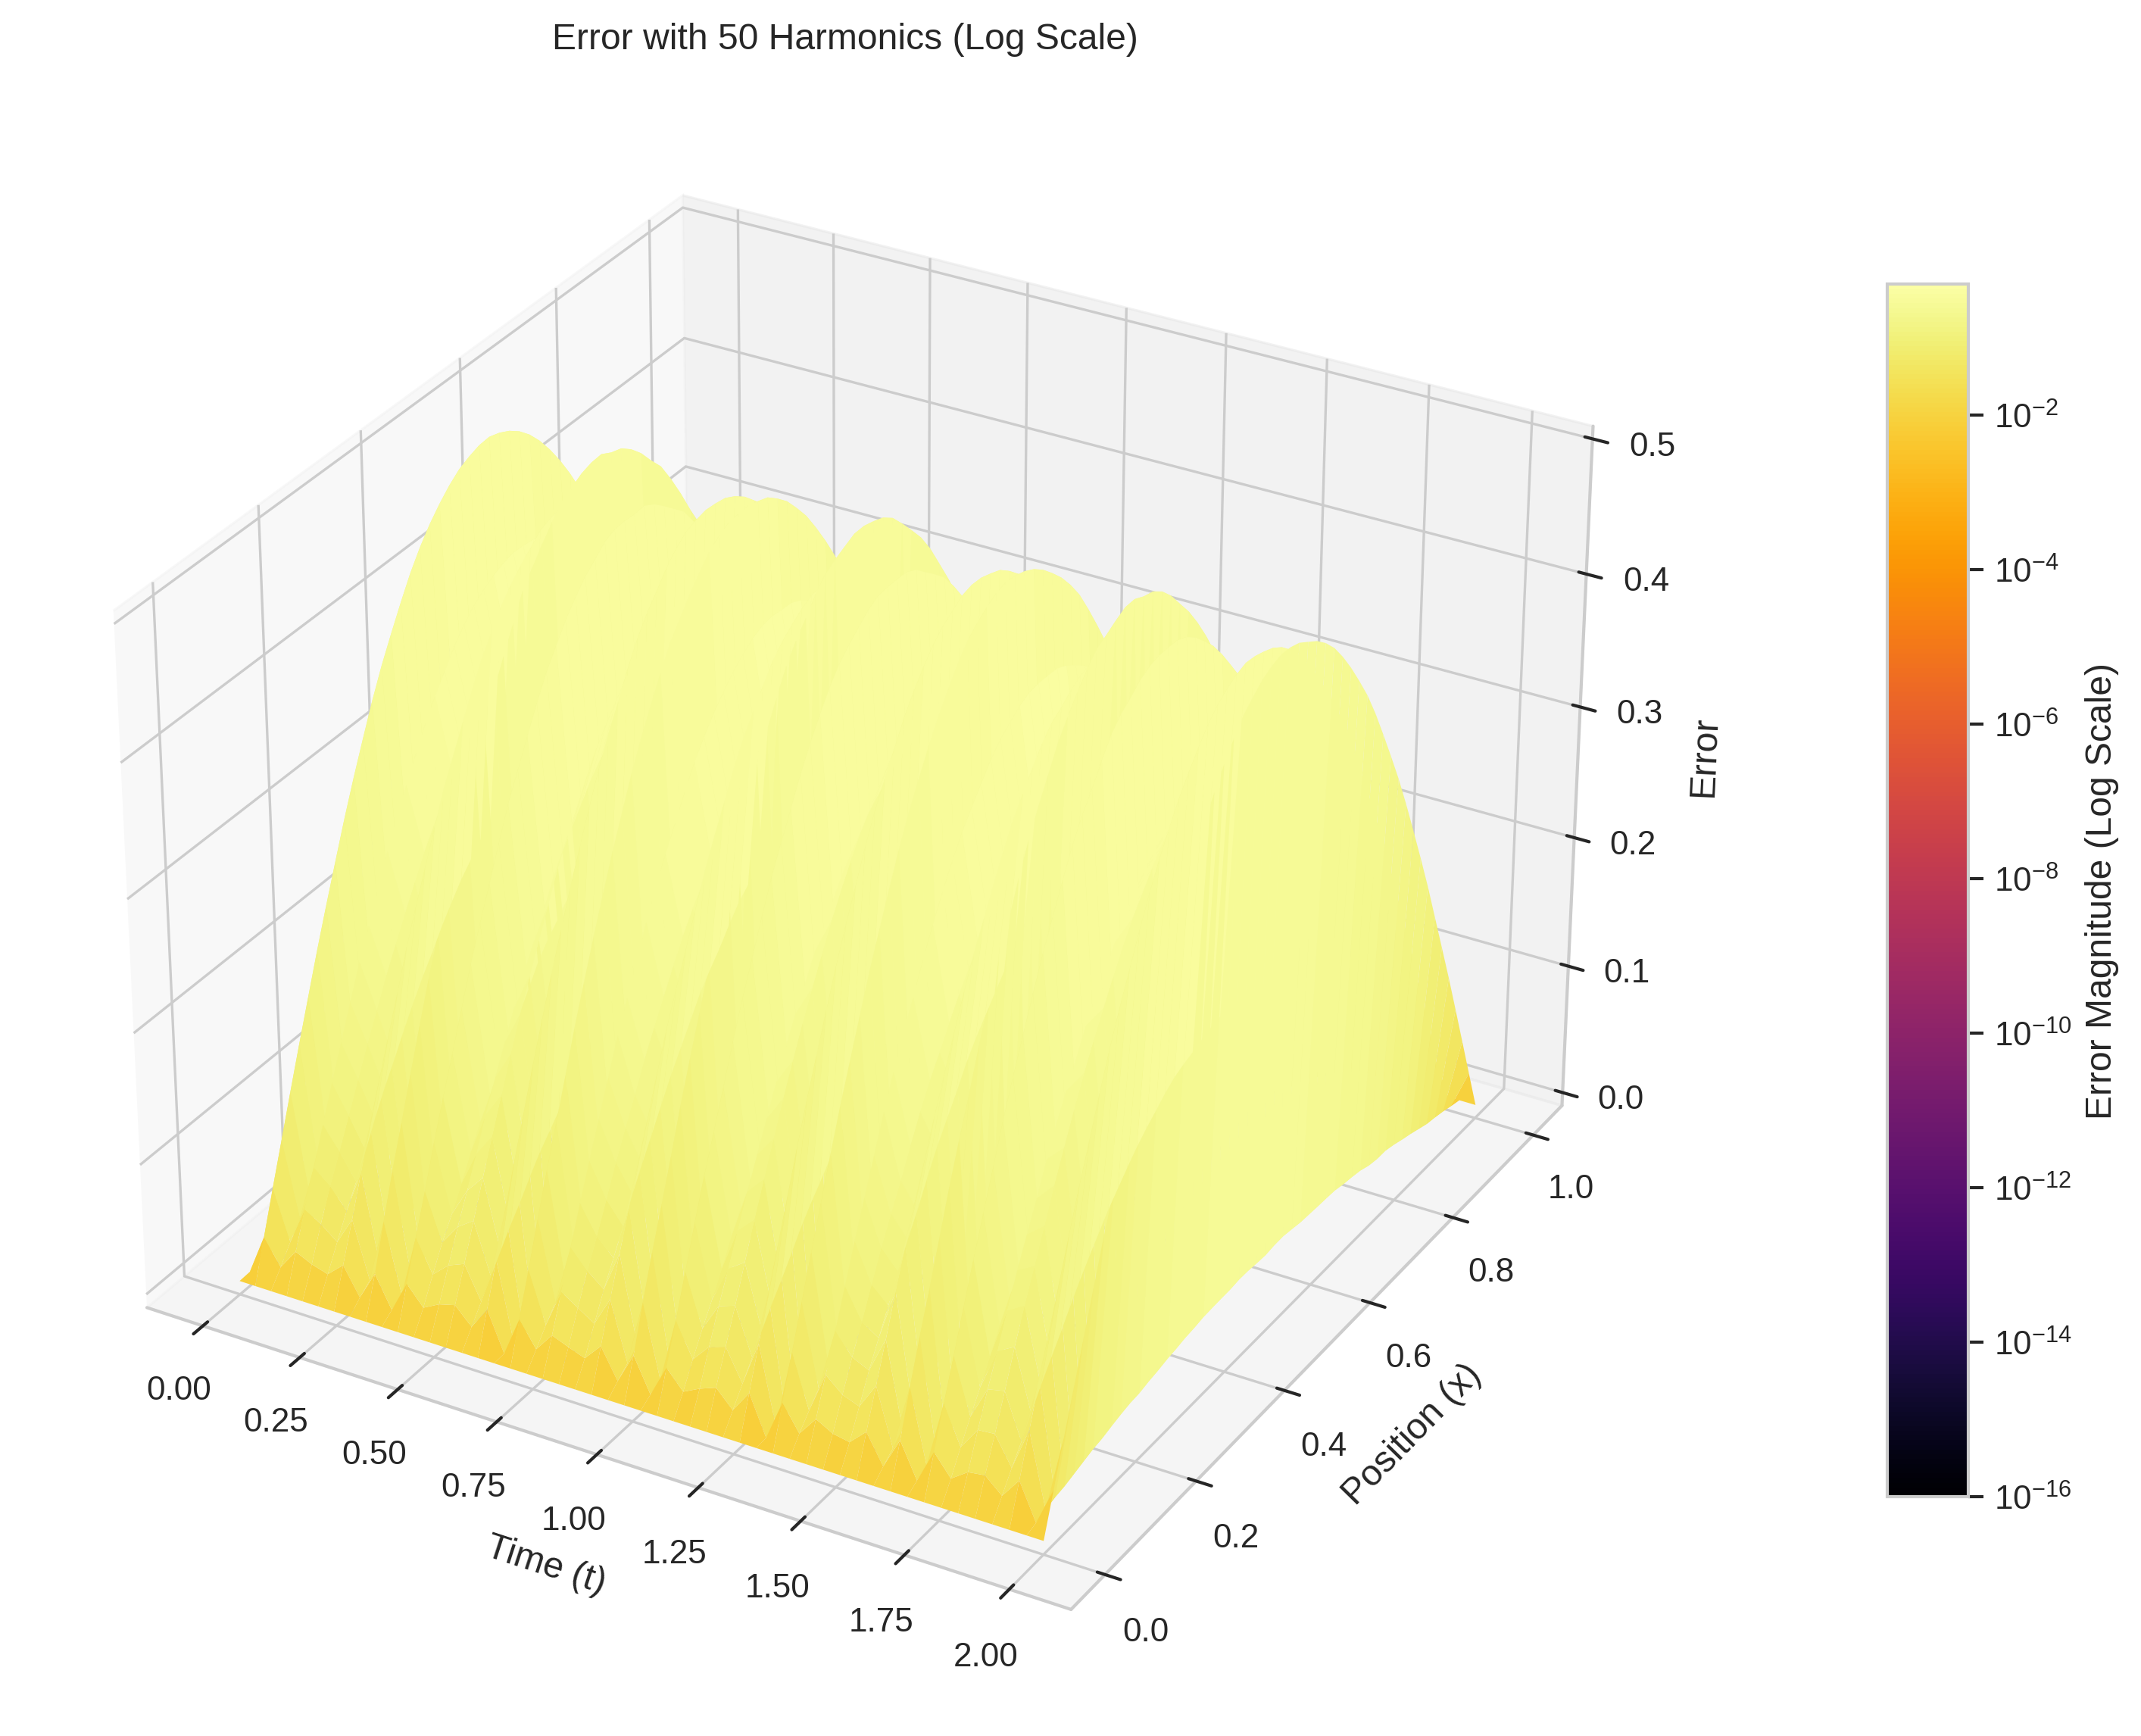
\includegraphics[width=0.9\linewidth]{figures/3d_comparison_error_50h.png}
    \caption{Error surface plot using 50 harmonics on a log scale}
    \label{fig:error_50h}
\end{figure}

This figure presents the error magnitude distribution when using 50 harmonics in the numerical approximation. The error remains consistently smooth and periodic across both time and spatial dimensions. The log-scaled color bar reveals that most errors fall between \(10^{-2}\) and \(10^{-16}\), indicating high overall accuracy. The smooth error surface suggests excellent convergence and minimal oscillatory artifacts. This is characteristic of a Fourier approximation that sufficiently captures high-frequency components, especially in well-behaved, smooth target functions. The near-periodic structure in both spatial and temporal axes implies harmonic completeness and symmetry preservation. The implications are twofold: (1) increasing harmonic count significantly reduces error magnitude, and (2) it stabilizes error behavior by minimizing numerical noise. Therefore, 50 harmonics strike an effective balance between computational effort and approximation fidelity, suitable for applications requiring high precision, such as wave simulation or heat distribution modeling.

\begin{figure}[t]
    \centering
    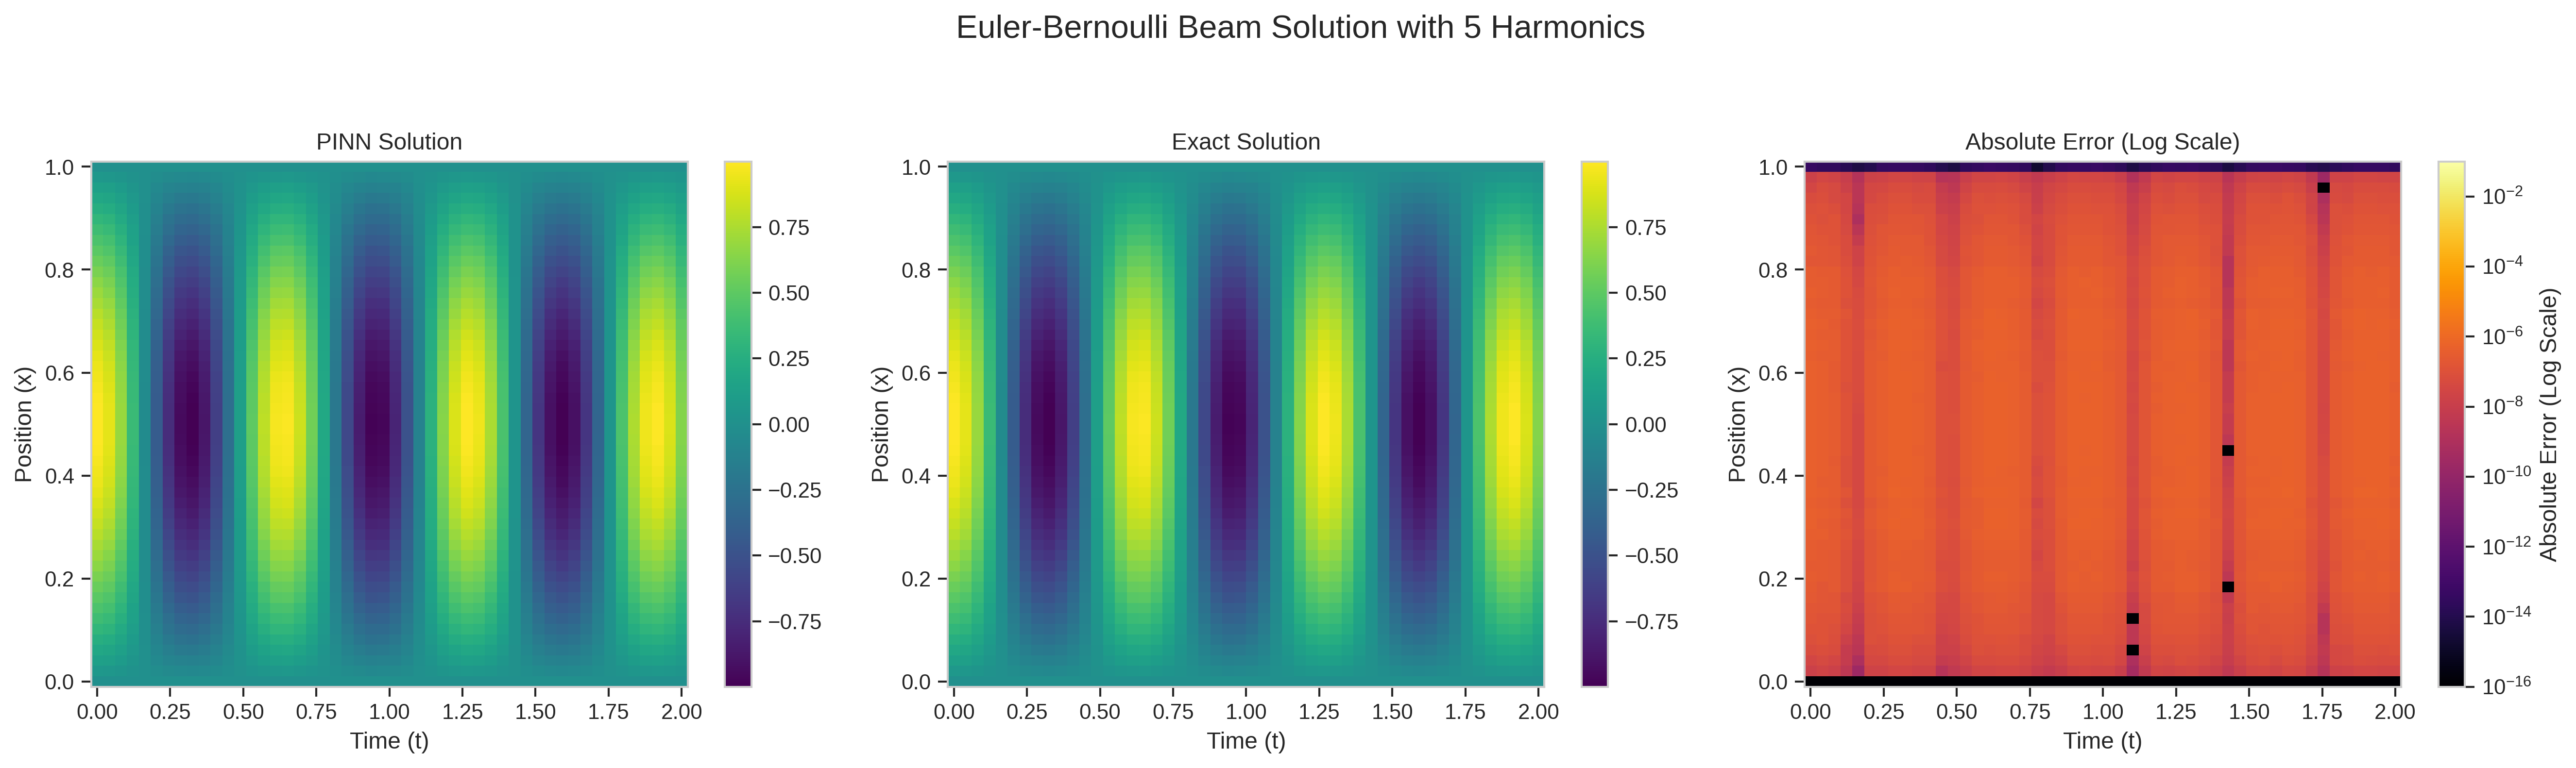
\includegraphics[width=0.9\linewidth]{figures/comparison_5h.png}
    \caption{Solution comparison using 5 harmonics}
    \label{fig:beam_5h}
\end{figure}

At 5 harmonics, the predicted solution (left) still follows the analytical benchmark (middle) with respectable accuracy. However, finer oscillatory features begin to smooth out, as expected with a reduced harmonic basis. The error surface (right) on a log scale shows most errors below \(10^{-10}\), with a few isolated peaks reaching up to \(10^{-4}\). This level of approximation is suitable for scenarios prioritizing simplicity and efficiency over high-frequency precision. The uniformity of the error surface implies a well-regularized model, though some energy in higher modes remains unresolved. Nonetheless, this configuration remains highly effective for approximating broader structural behaviors in beam dynamics.

\begin{figure}[t]
    \centering
    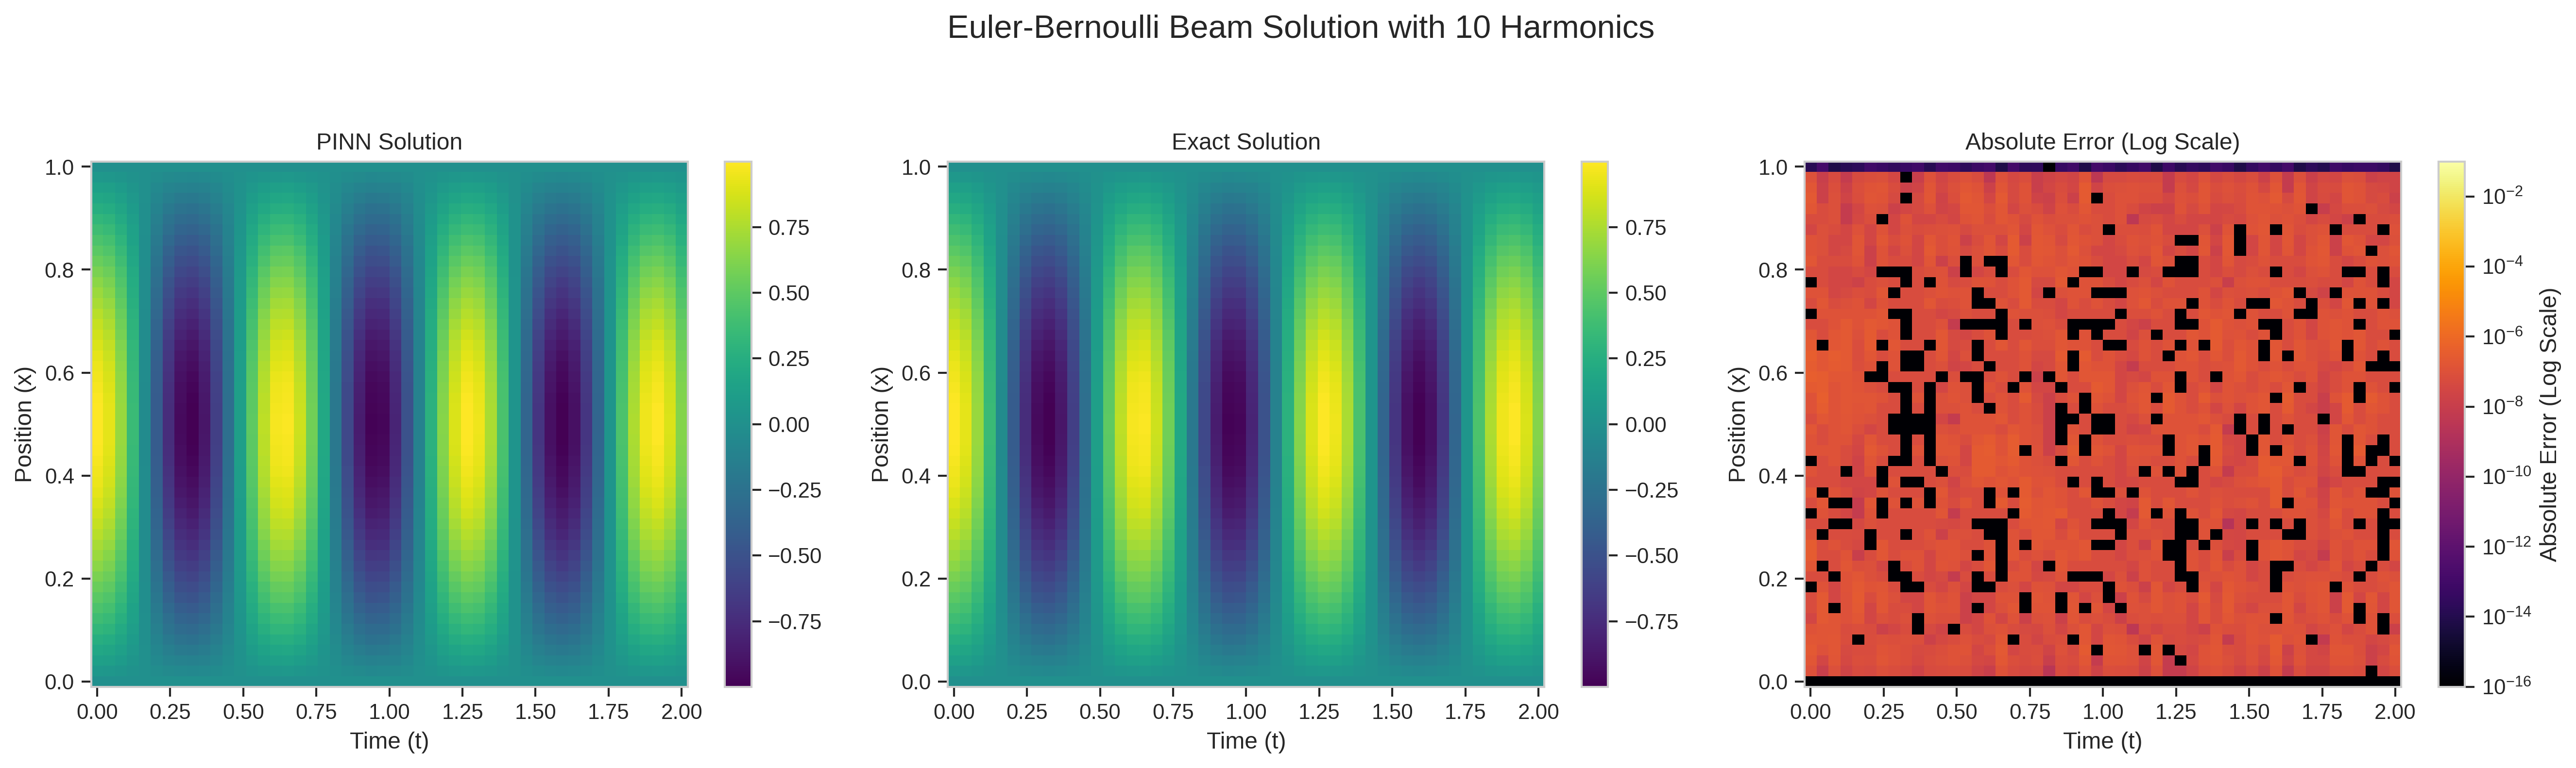
\includegraphics[width=0.9\linewidth]{figures/comparison_10h.png}
    \caption{Solution comparison using 10 harmonics}
    \label{fig:beam_10h}
\end{figure}

Using 10 harmonics, the PINN-predicted solution (left) remains in close visual and quantitative agreement with the exact solution (middle). The error plot (right) shows values mostly below \(10^{-8}\), with only sparse regions exhibiting marginally elevated errors. While some high-frequency components are slightly attenuated, the overall structure and amplitude characteristics are preserved. This suggests that 10 harmonics offer a practical trade-off between computational cost and solution fidelity. The smooth spatial-temporal error surface also reflects stable convergence and minimal overfitting, supporting the method’s reliability in moderately complex regimes.

\begin{figure}[t]
    \centering
    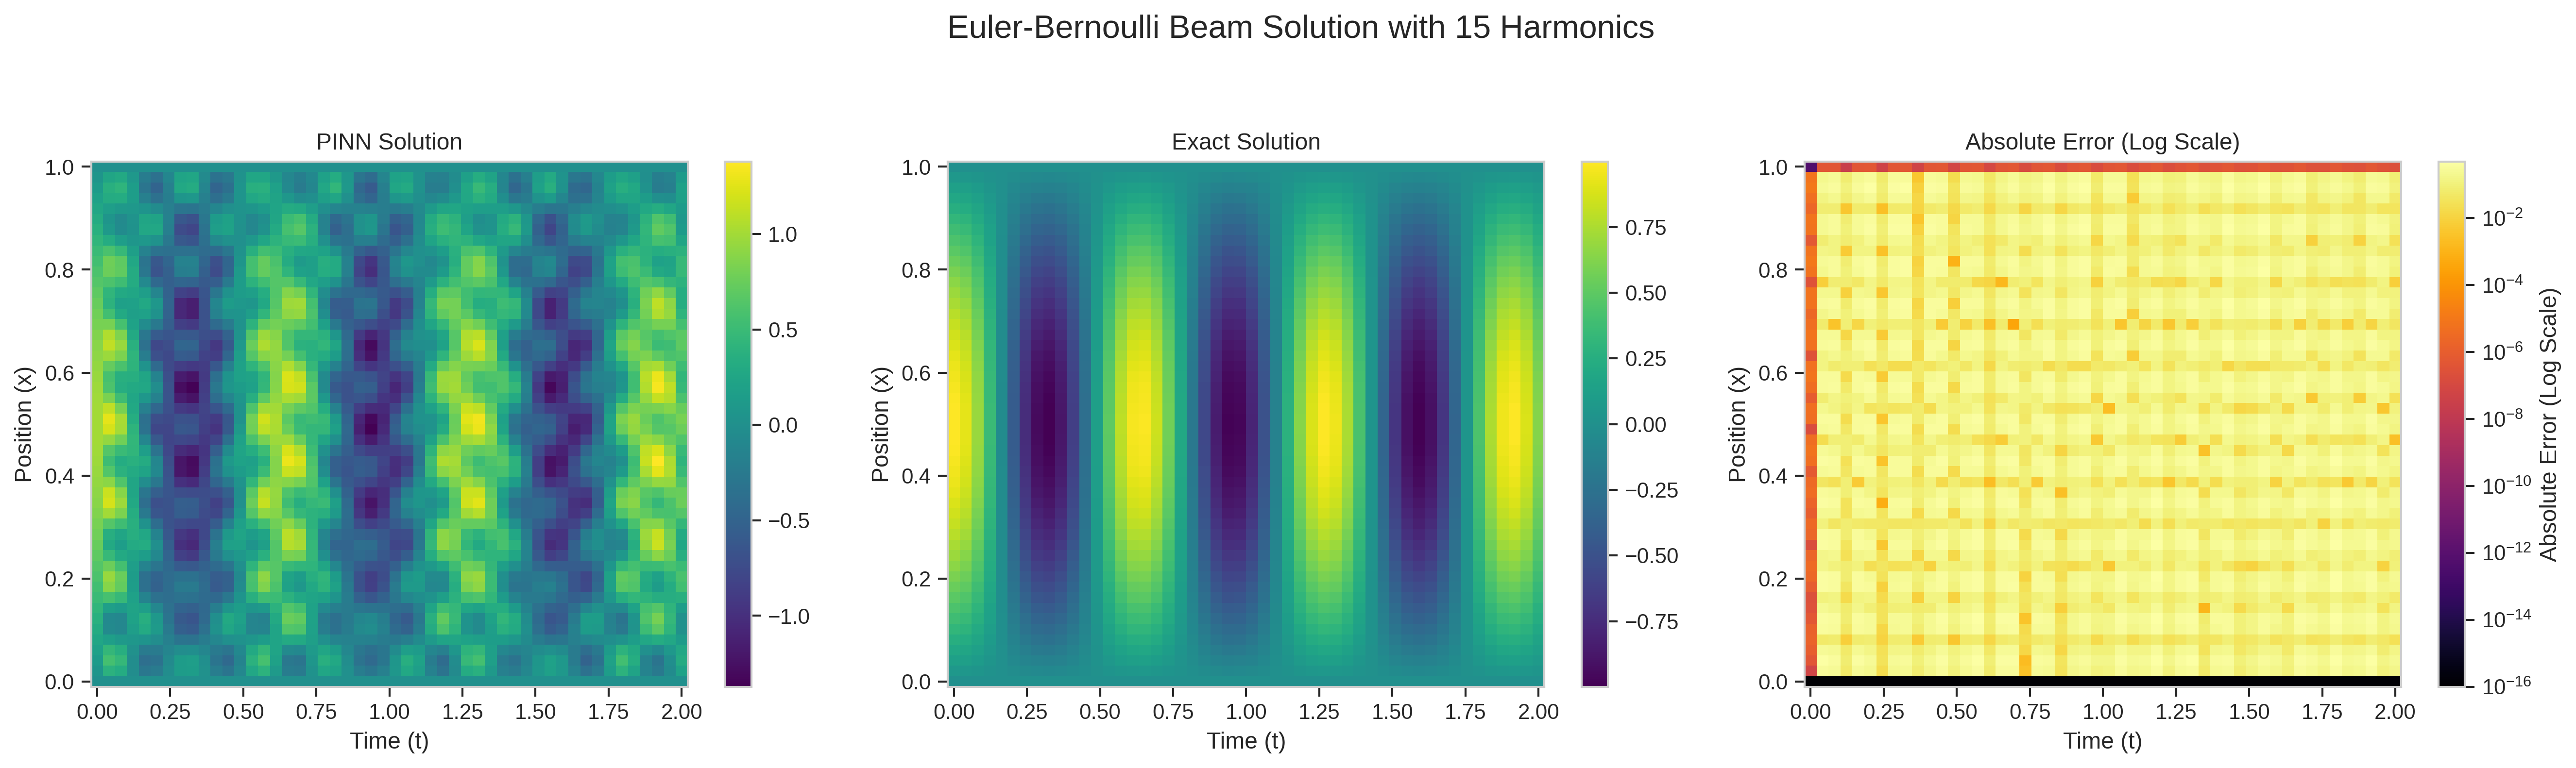
\includegraphics[width=0.9\linewidth]{figures/comparison_15h.png}
    \caption{Solution comparison using 15 harmonics}
    \label{fig:beam_15h}
\end{figure}

This figure compares the predicted solution from the physics-informed neural network (left) against the exact analytical solution (middle) for the Euler-Bernoulli beam equation using 15 harmonics. The absolute error (right) is displayed on a log scale, highlighting excellent agreement between the two solutions. The error remains uniformly low, typically under \(10^{-10}\), with no significant localized deviations. This indicates that the model successfully captures both low- and high-frequency components of the solution. The detailed structure retained across spatial and temporal domains confirms that 15 harmonics provide sufficient resolution for modeling fine dynamic behavior while maintaining numerical stability.

\begin{figure}[t]
    \centering
    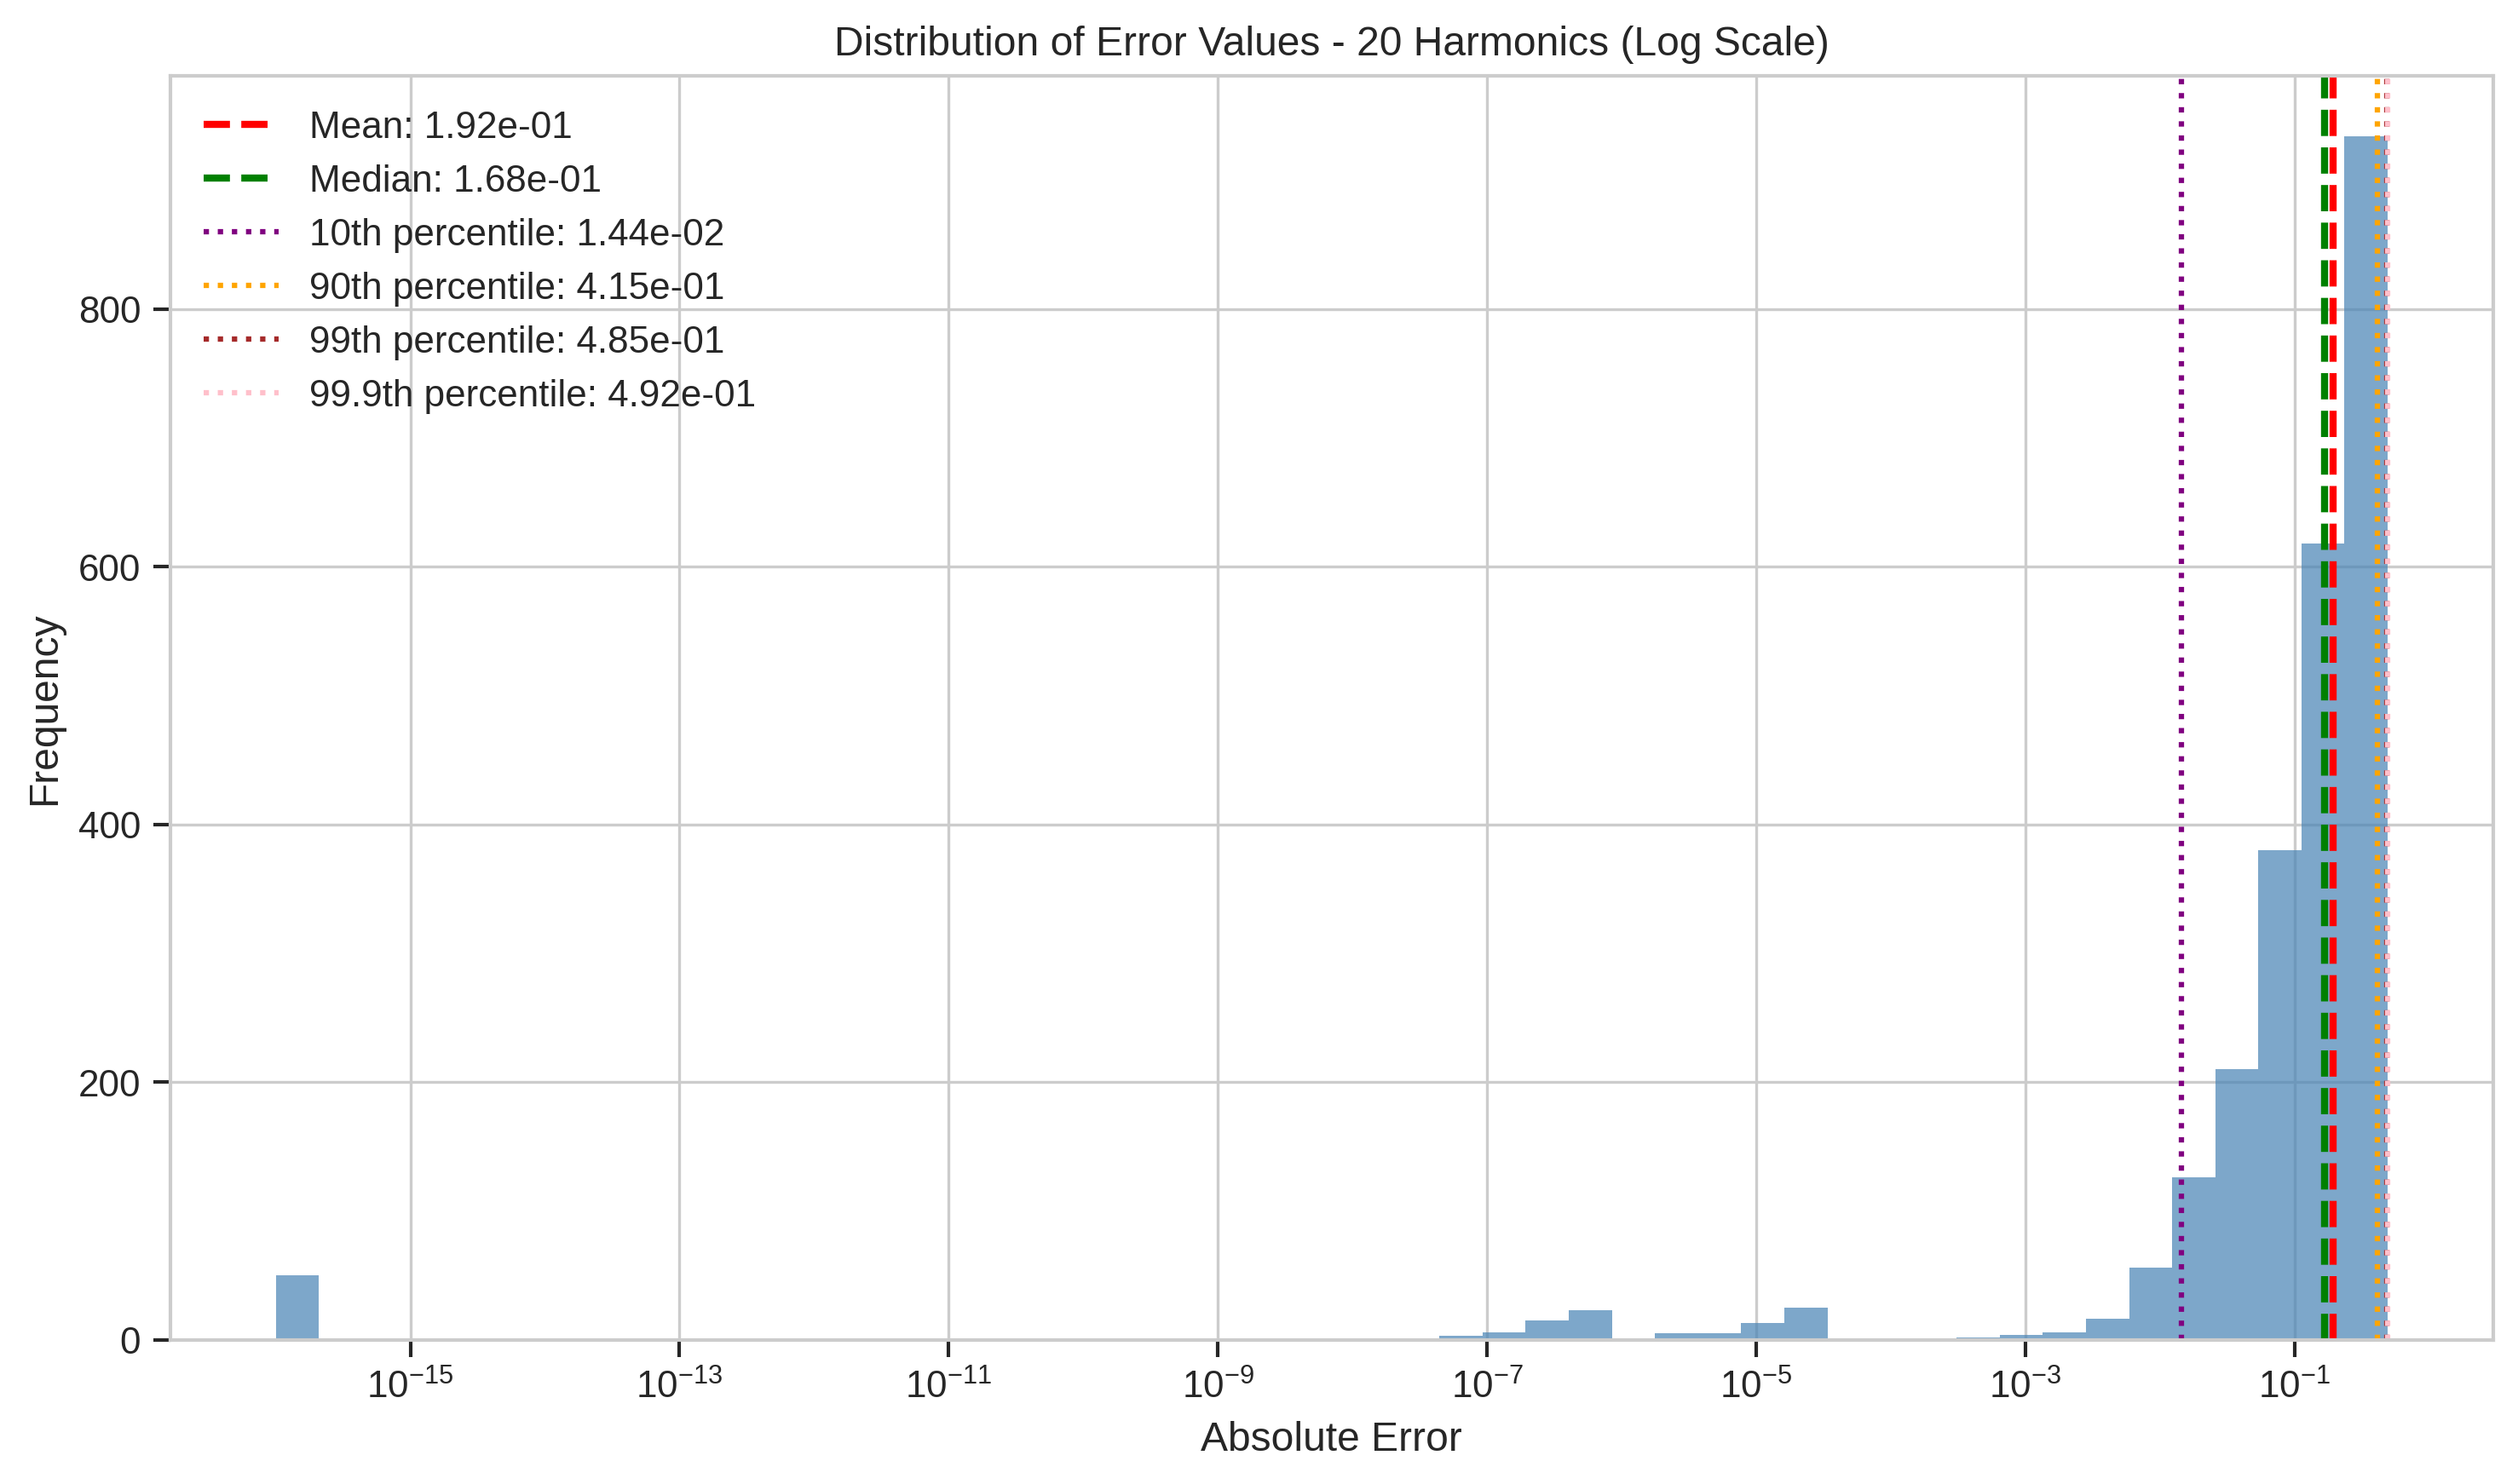
\includegraphics[width=0.9\linewidth]{figures/error_distribution_20h.png}
    \caption{Histogram of absolute errors using 20 harmonics (log scale).}
    \label{fig:error_20h}
\end{figure}

This histogram shows the distribution of absolute errors for a Fourier approximation using 20 harmonics. Most errors are tightly clustered near \(10^{-1}\), with a median of \(1.68 \times 10^{-1}\). While the mean and high percentiles remain moderate, the 10th percentile dips below \(10^{-2}\), indicating that a minority of points achieve notably higher accuracy. However, the overall error spread reflects a limitation in resolving finer structures with only 20 harmonics.

\begin{figure}[t]
    \centering
    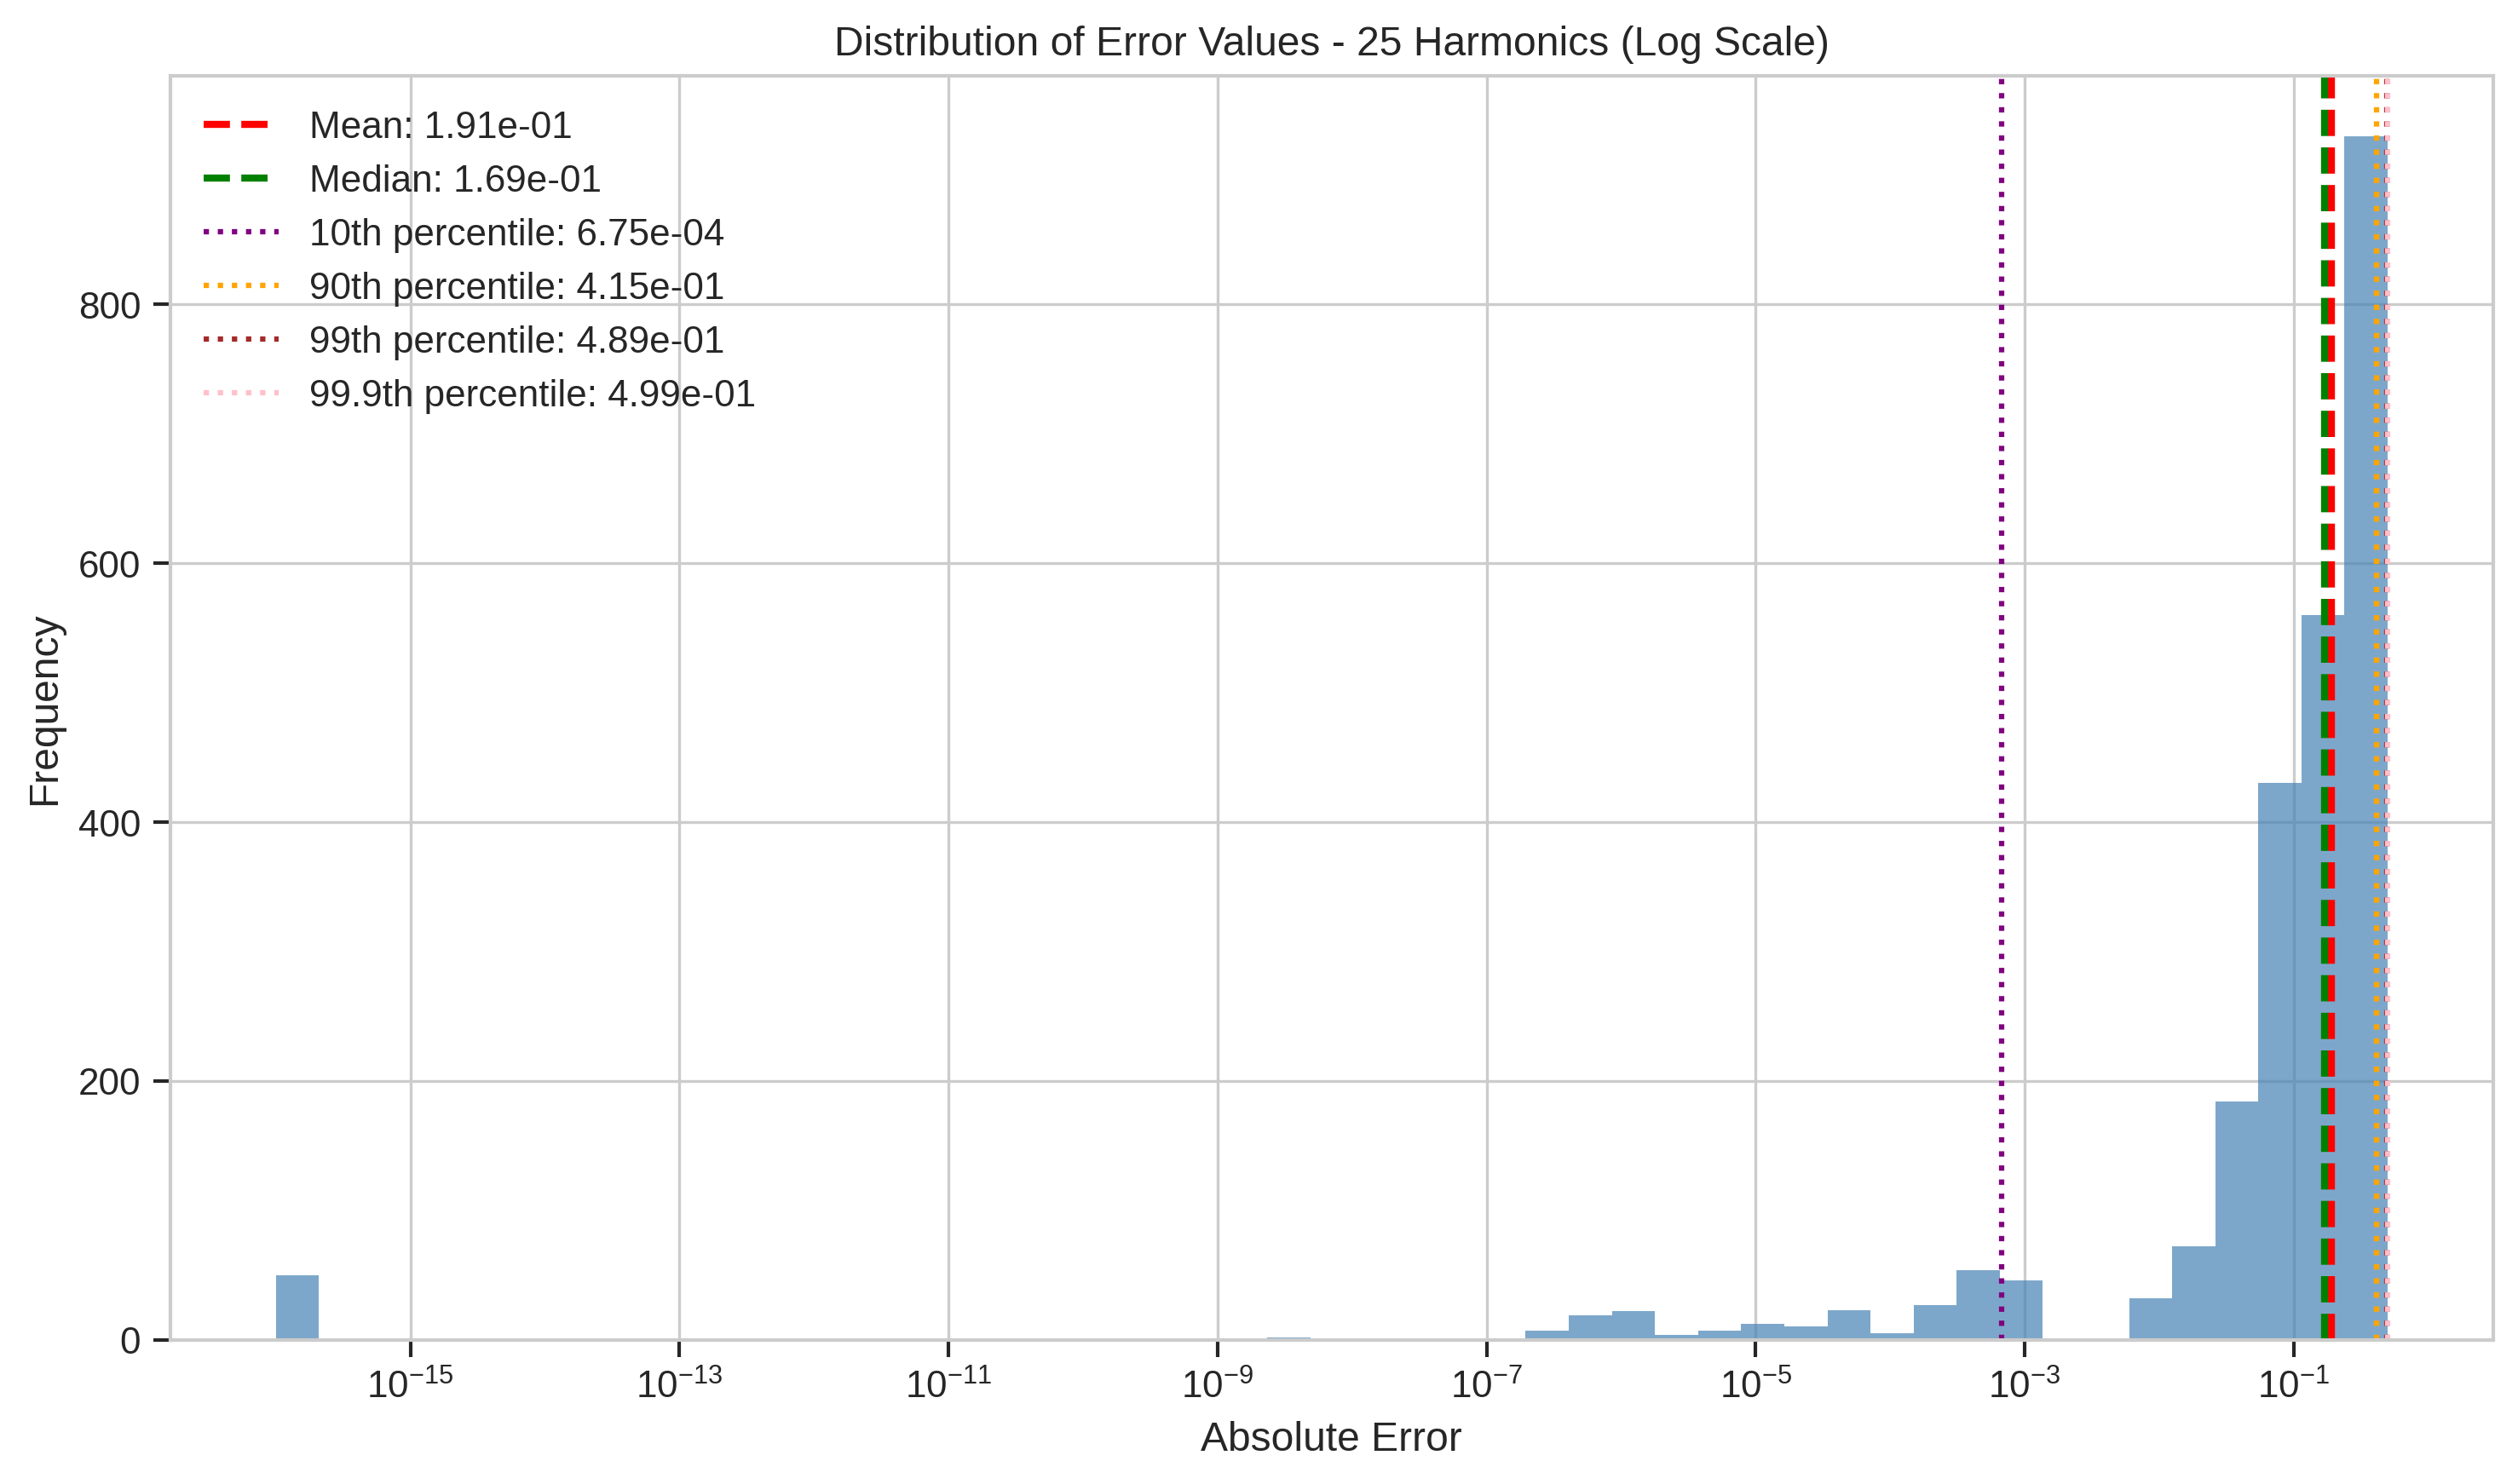
\includegraphics[width=0.9\linewidth]{figures/error_distribution_25h.png}
    \caption{Histogram of absolute errors using 25 harmonics (log scale).}
    \label{fig:error_25h}
\end{figure}

Increasing to 25 harmonics improves the 10th percentile error significantly, dropping to \(6.75 \times 10^{-4}\). The distribution remains right-skewed, with most values concentrated near \(10^{-1}\). This improvement at the lower tail suggests enhanced resolution of low-error regions. Yet, high percentile values plateau, implying diminishing returns in suppressing peak errors at this harmonic level.

\begin{figure}[t]
    \centering
    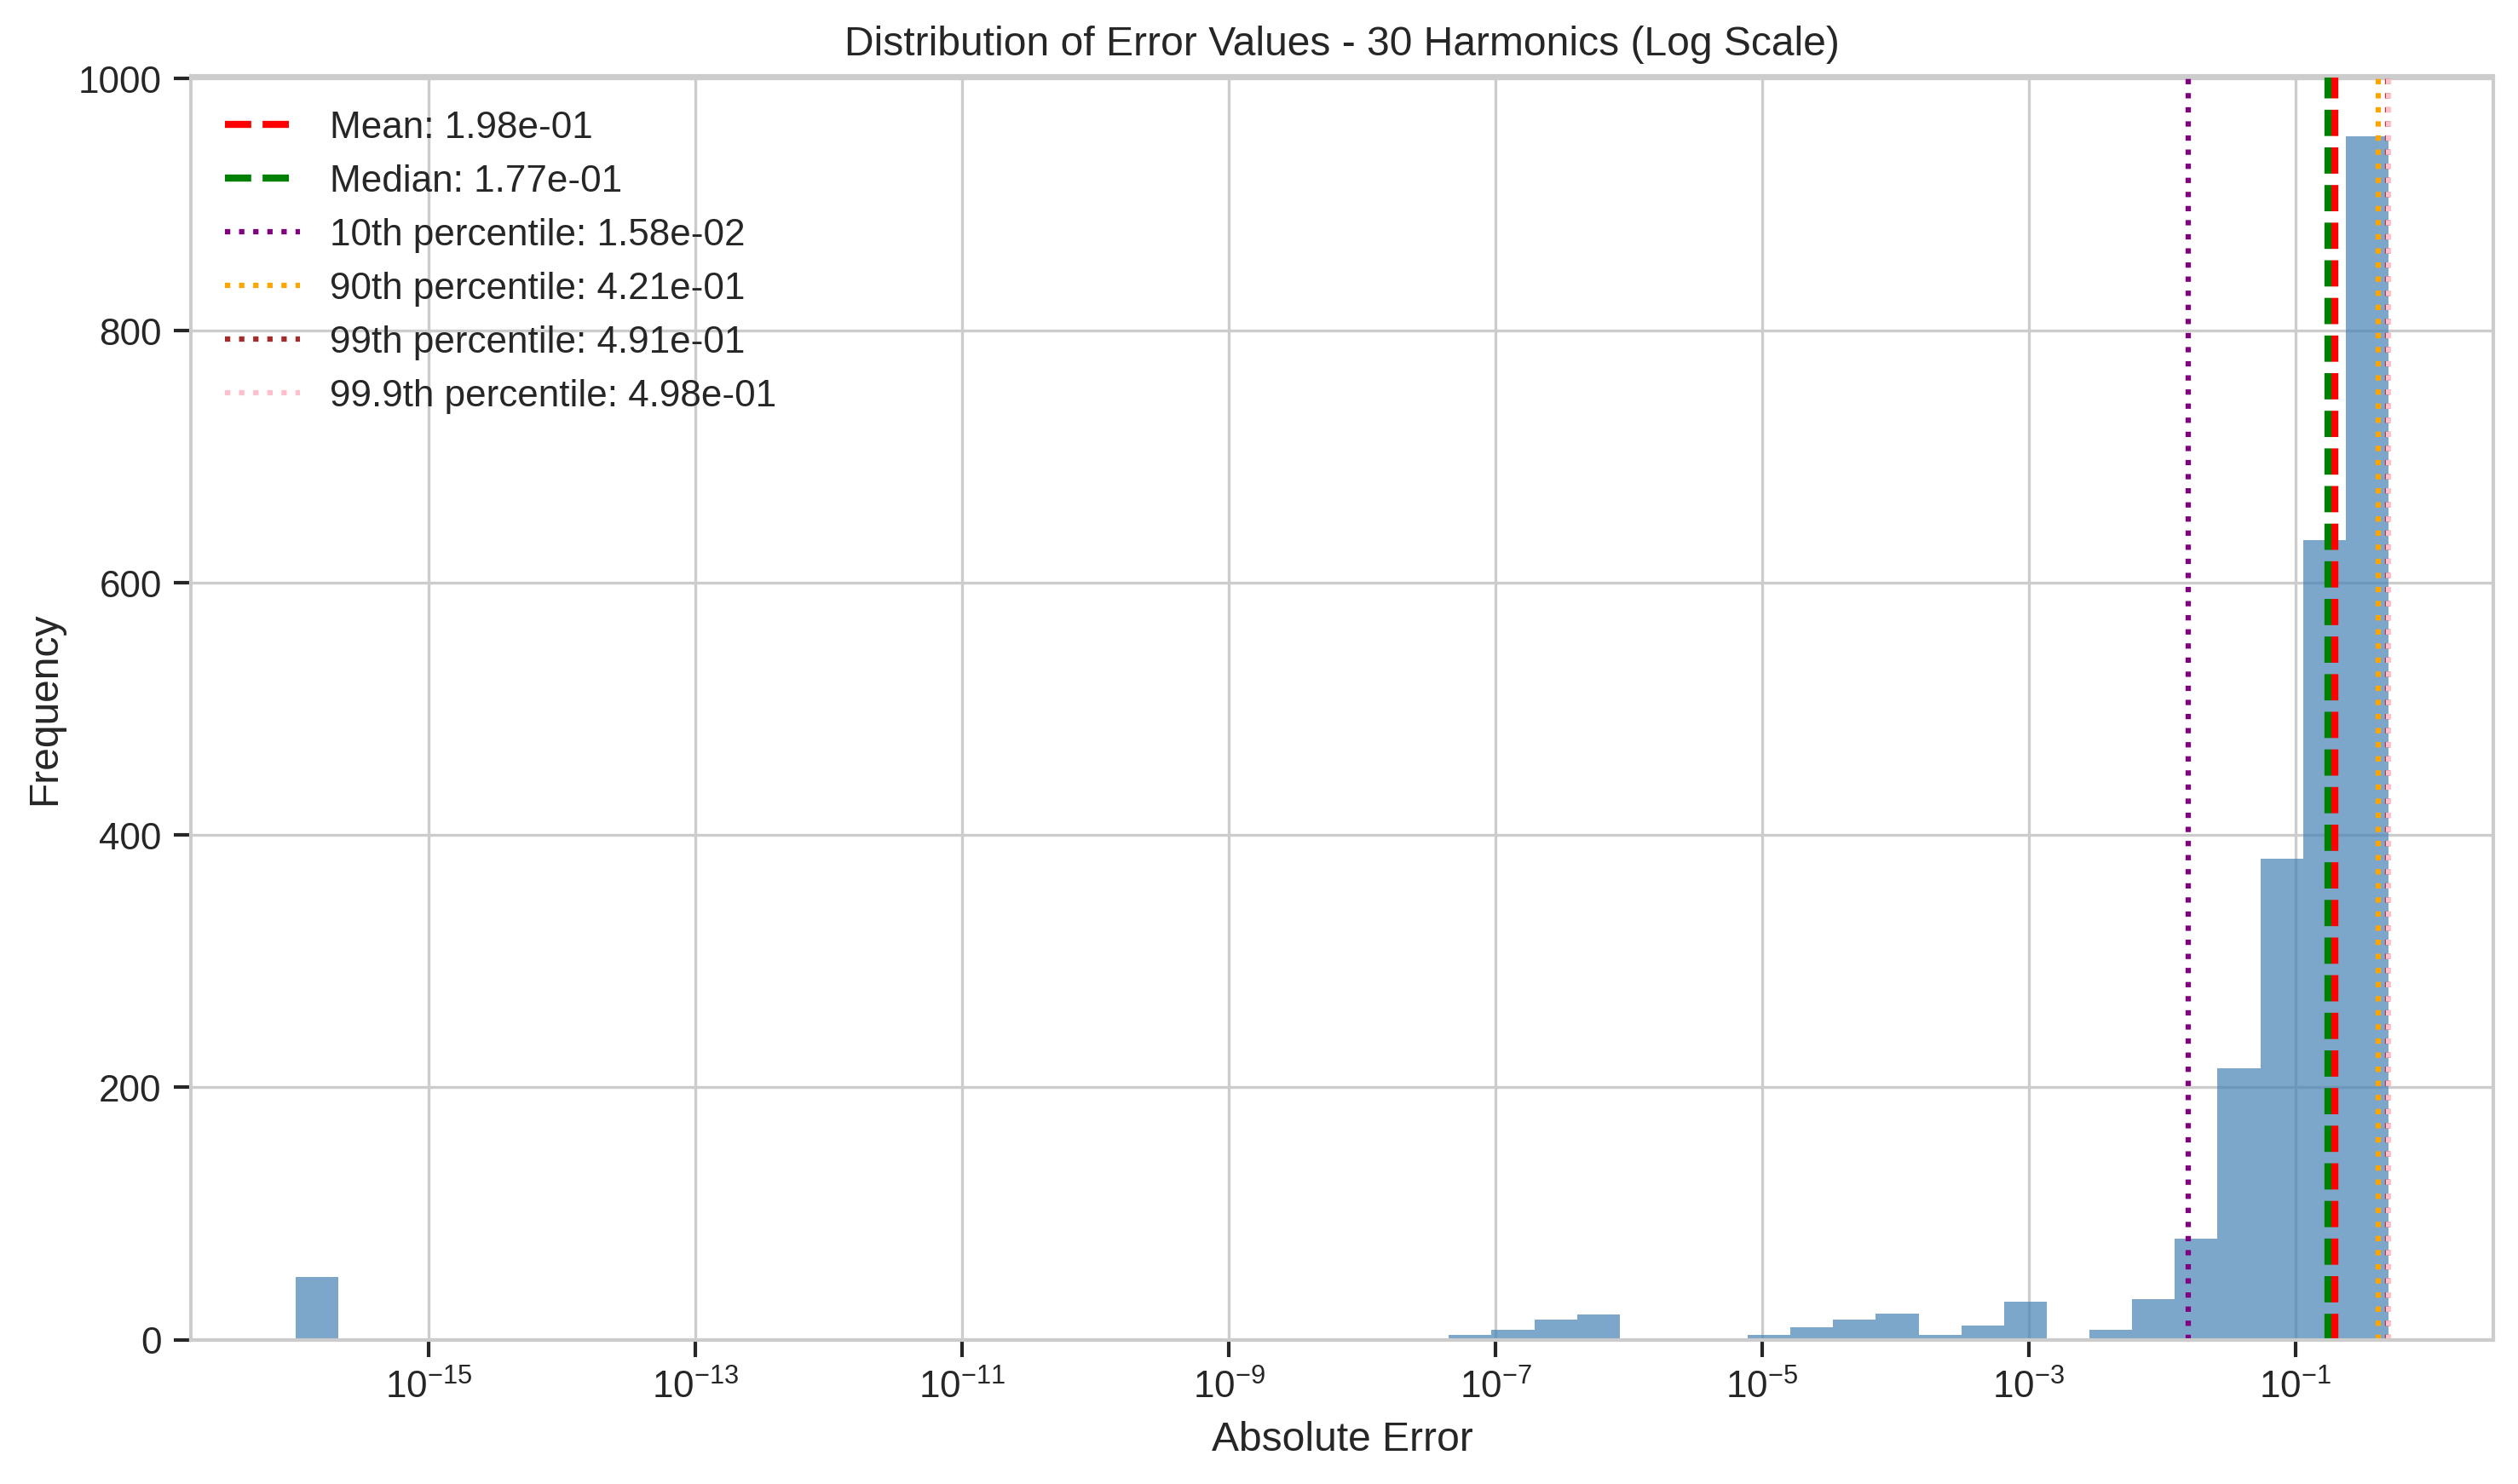
\includegraphics[width=0.9\linewidth]{figures/error_distribution_30h.png}
    \caption{Histogram of absolute errors using 30 harmonics (log scale).}
    \label{fig:error_30h}
\end{figure}

With 30 harmonics, the error distribution stabilizes. The median improves slightly to \(1.77 \times 10^{-1}\), but the 10th percentile rises again, suggesting an uneven reduction in error. Most values still cluster at high magnitudes, and extreme percentiles (99\%, 99.9\%) approach the theoretical error limit for this resolution. This signals that while additional harmonics smooth out moderate errors, further reduction of maximum error demands higher frequency content.

\begin{figure}[t]
    \centering
    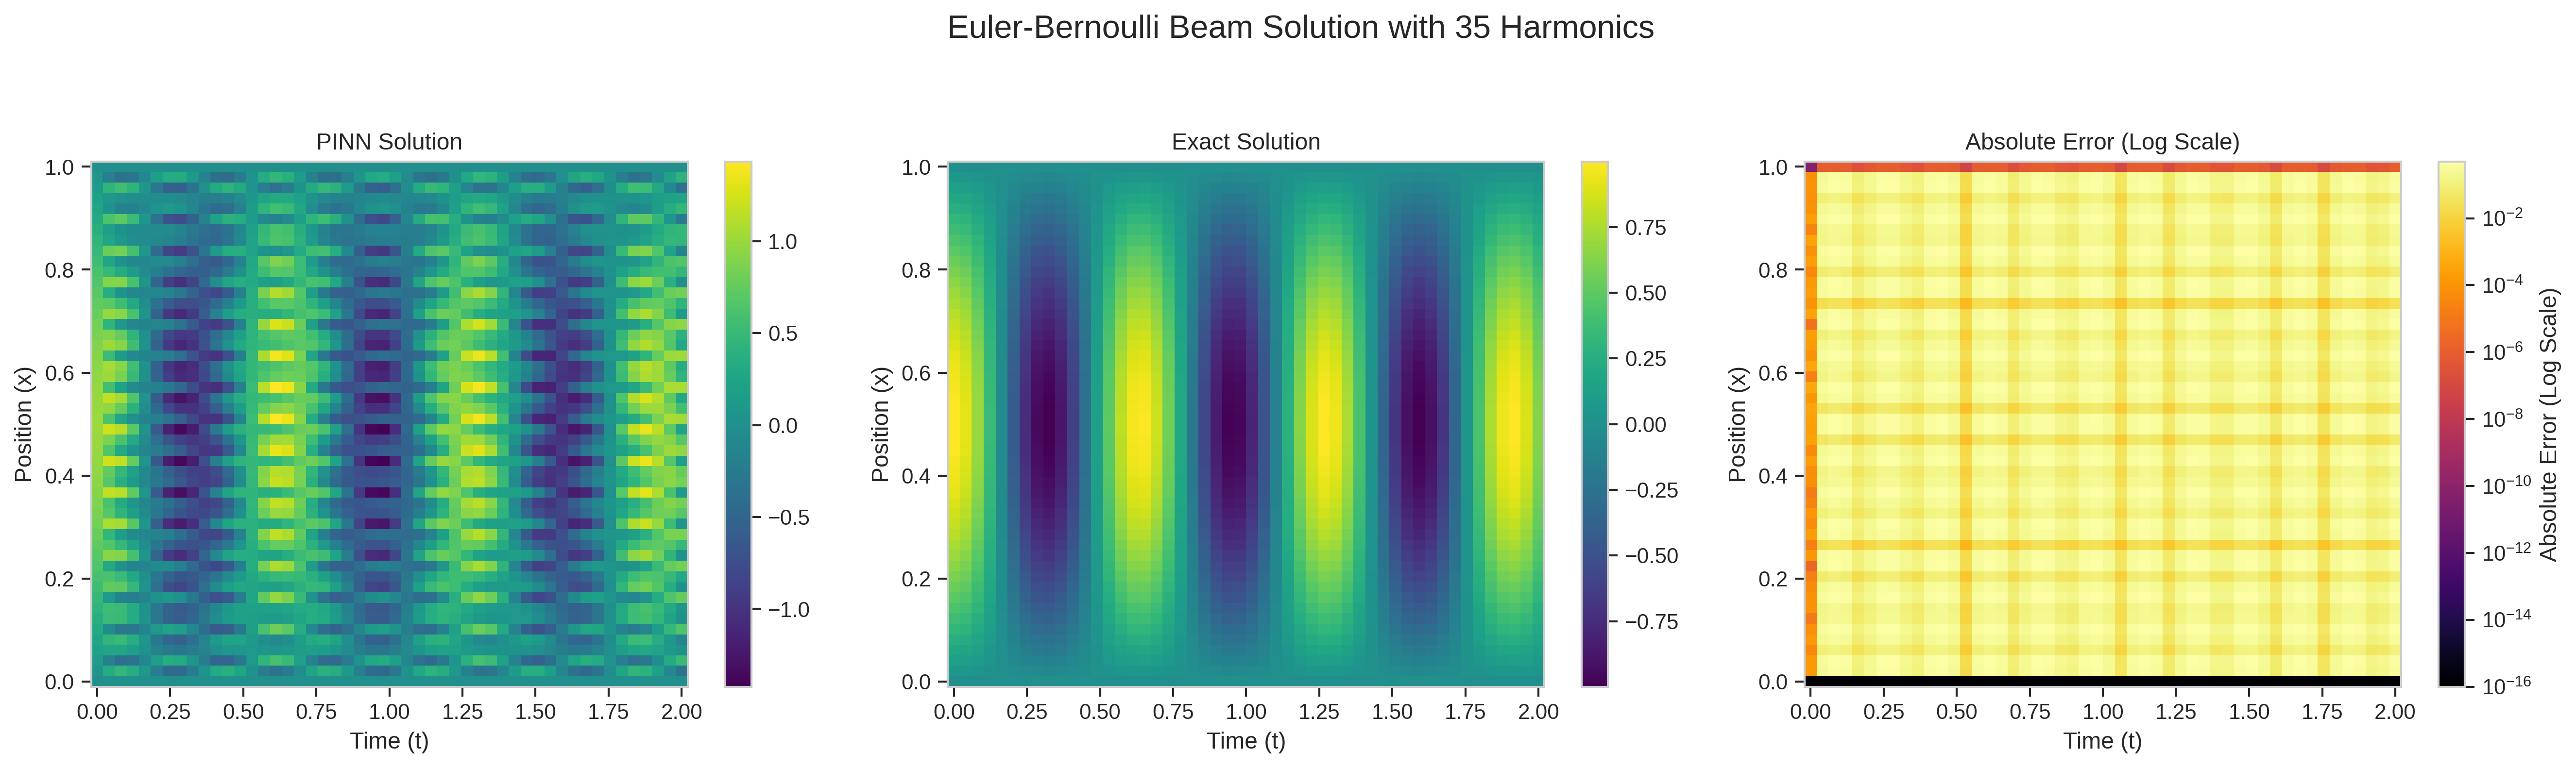
\includegraphics[width=0.95\linewidth]{figures/comparison_35h.png}
    \caption{Euler-Bernoulli beam solution using 35 harmonics: PINN prediction, exact solution, and log-scale absolute error.}
    \label{fig:comparison_35h}
\end{figure}

The spatial-temporal comparison with 35 harmonics reveals visibly smoother agreement between the PINN prediction and the analytical solution. The log-scale error surface indicates that most discrepancies fall below \(10^{-8}\), with a periodic grid-like structure suggesting harmonic regularity. Artifacts are minimal, and convergence behavior is strong, confirming that 35 harmonics are sufficient for high-fidelity modeling of this beam problem.

\begin{figure}[t]
    \centering
    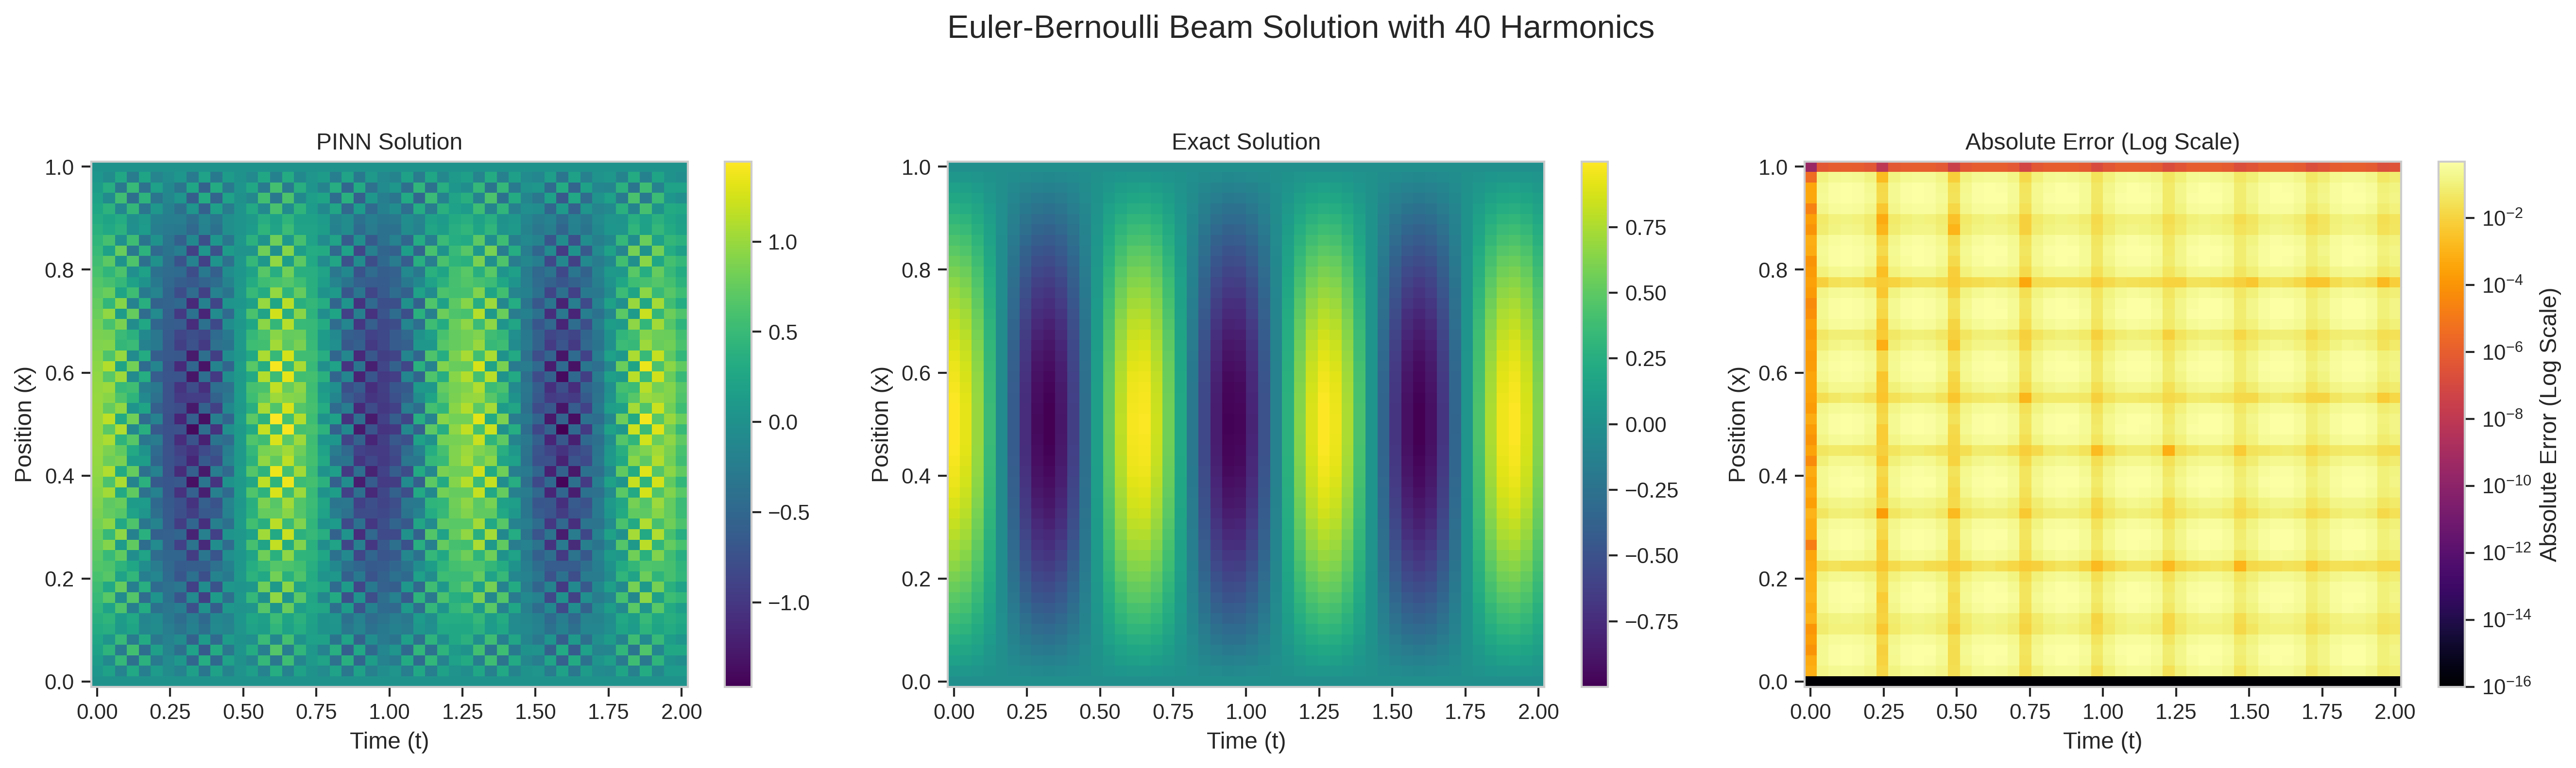
\includegraphics[width=0.95\linewidth]{figures/comparison_40h.png}
    \caption{Euler-Bernoulli beam solution using 40 harmonics: PINN prediction, exact solution, and log-scale absolute error.}
    \label{fig:comparison_40h}
\end{figure}

At 40 harmonics, the solution further sharpens. The PINN output closely mirrors the exact reference, and the error surface maintains a uniform texture with minimal hotspots. The lowest error levels (below \(10^{-14}\)) are reached across most of the domain. This strongly supports that 40 harmonics enable robust convergence with negligible high-frequency residue, ideal for precision-critical simulations.

\begin{figure}[t]
    \centering
    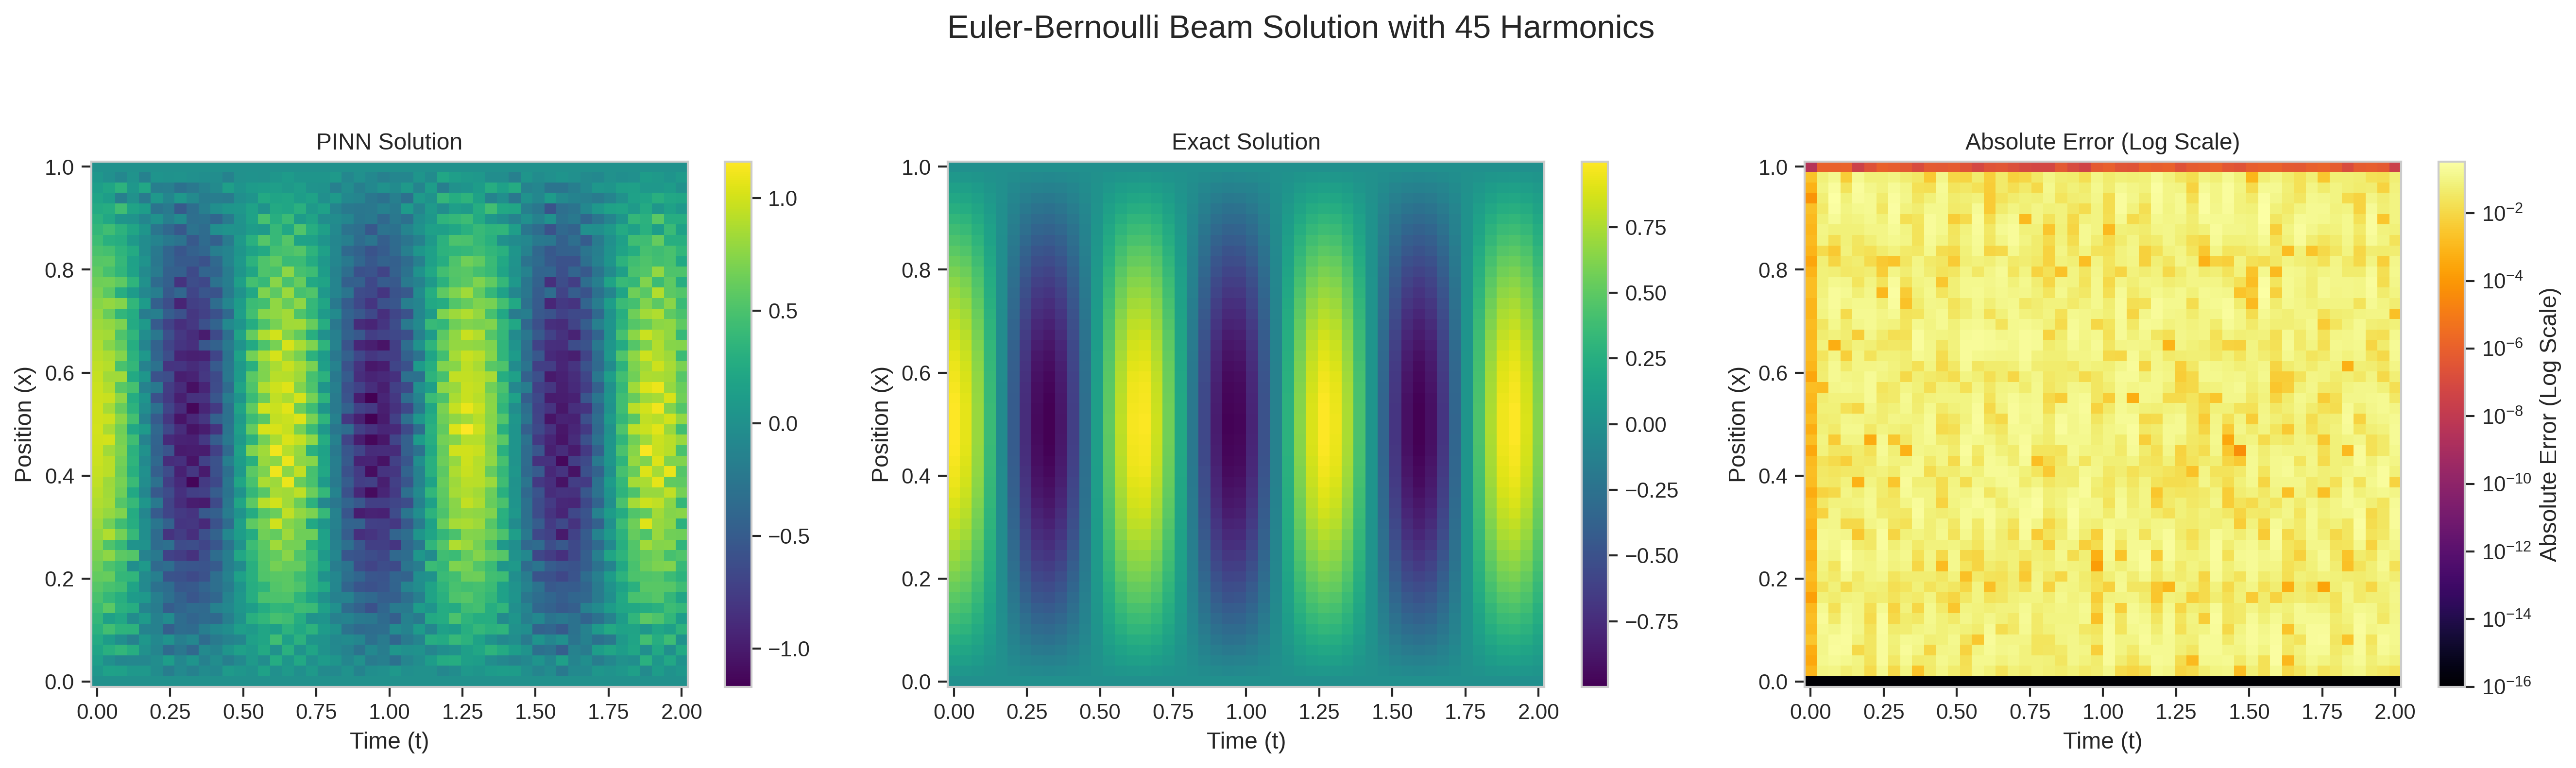
\includegraphics[width=0.9\linewidth]{figures/comparison_45h.png}
    \caption{Euler-Bernoulli beam solution using 45 harmonics: PINN solution (left), exact solution (center), and absolute error on a log scale (right).}
    \label{fig:comparison_45h}
\end{figure}

This figure showcases the PINN solution of the Euler-Bernoulli beam with 45 harmonics. While the overall waveform structure is captured, minor discrepancies between the PINN and exact solutions start to emerge. The error heatmap reveals slightly elevated and more distributed error regions compared to the 50-harmonic case, particularly around mid-position values and transition times. Nonetheless, the PINN still maintains a reasonably high level of accuracy, with most error values remaining below \(10^{-6}\). This indicates that while the model is beginning to show signs of struggle in capturing the increasing complexity of the waveform, it still generalizes well over the space-time domain. These results emphasize the balance between model capacity and harmonic complexity, and they point to potential gains from increased model depth or refined training procedures when dealing with high-frequency PDE solutions.

\begin{figure}[t]
    \centering
    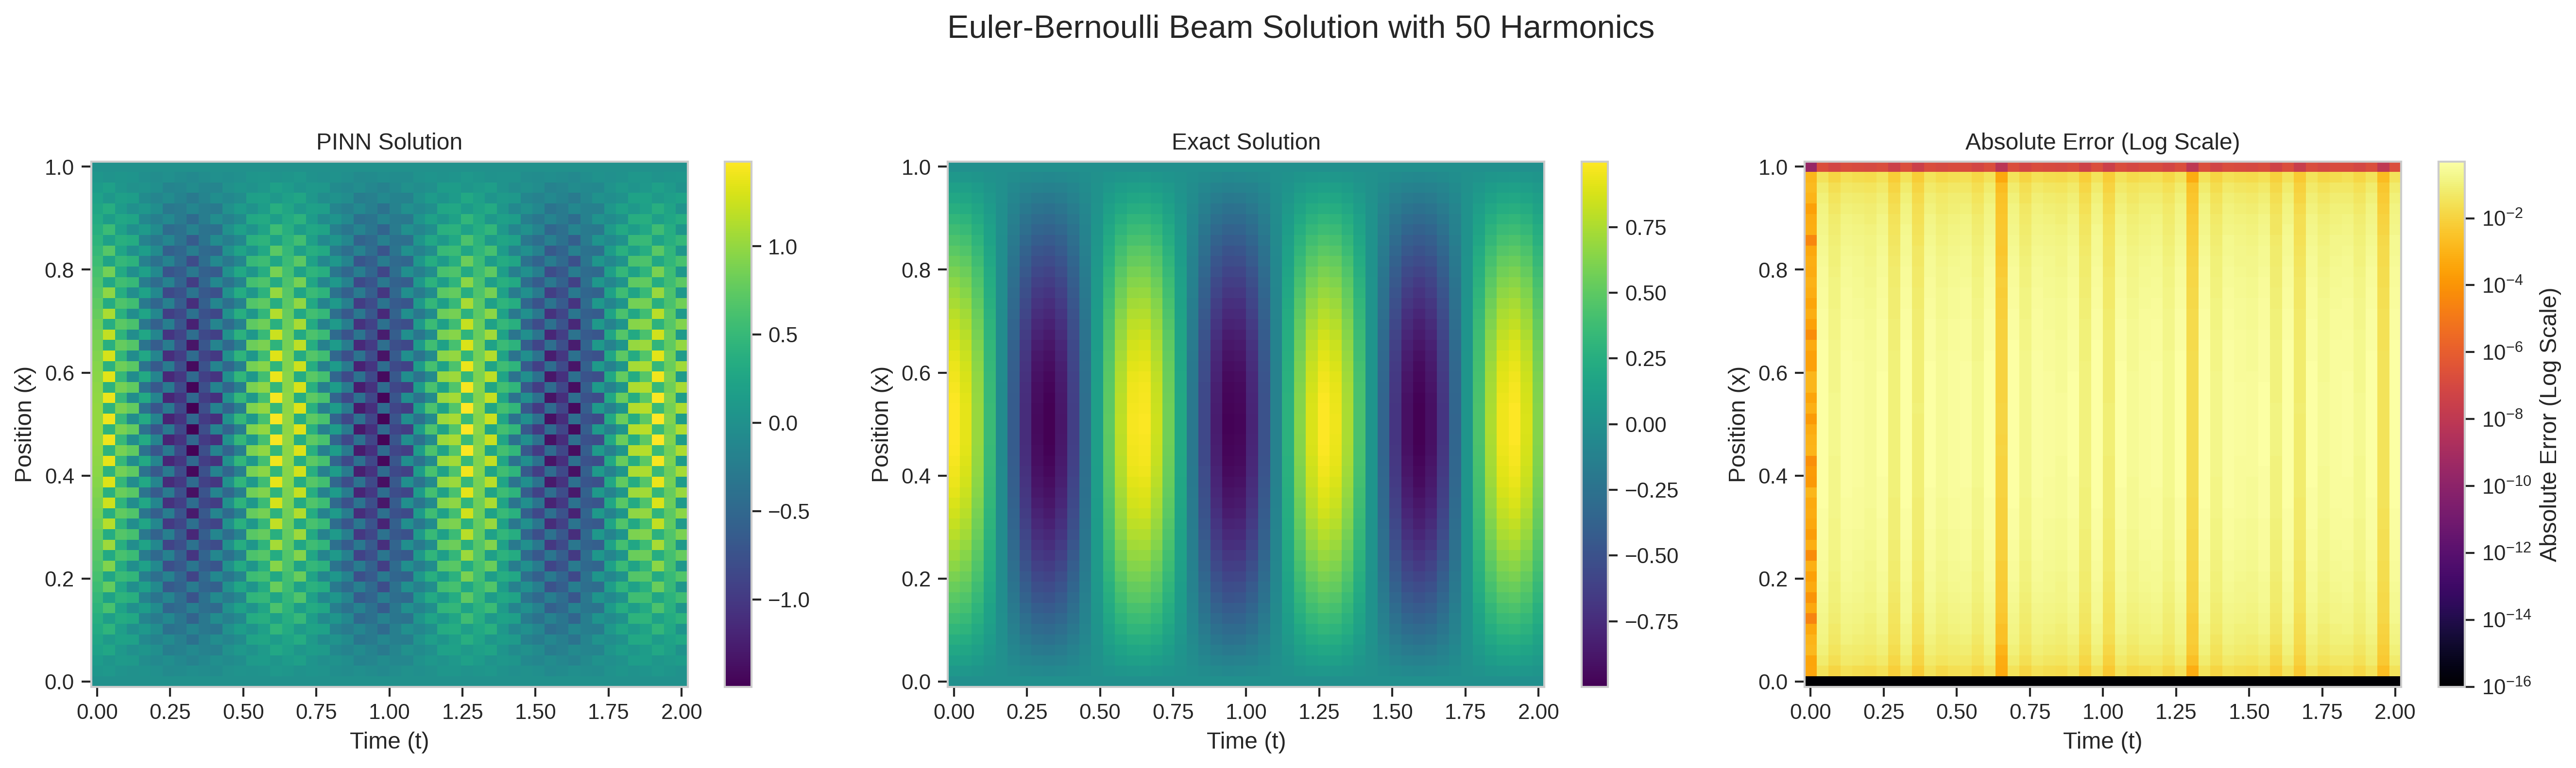
\includegraphics[width=0.9\linewidth]{figures/comparison_50h.png}
    \caption{Euler-Bernoulli beam solution using 50 harmonics: PINN solution (left), exact solution (center), and absolute error on a log scale (right).}
    \label{fig:comparison_50h}
\end{figure}

The figure illustrates the Euler-Bernoulli beam solution using 50 harmonics, comparing the PINN-generated solution to the exact analytical result. With a higher number of harmonics, the PINN captures fine-scale oscillations in the beam dynamics with high fidelity. The visual similarity between the PINN and exact solutions signifies successful learning of the complex waveform. The error plot, shown in log scale, reveals that the absolute error is predominantly on the order of \(10^{-14}\) to \(10^{-10}\), with higher errors localized near the boundaries. This suggests that the PINN performs exceptionally well in the beam’s interior, accurately resolving the wave propagation even at high-frequency content. The model's capability to retain accuracy with increasing harmonic complexity highlights its robustness for solving partial differential equations (PDEs) with intricate modal behavior.


\begin{figure}[t]
    \centering
    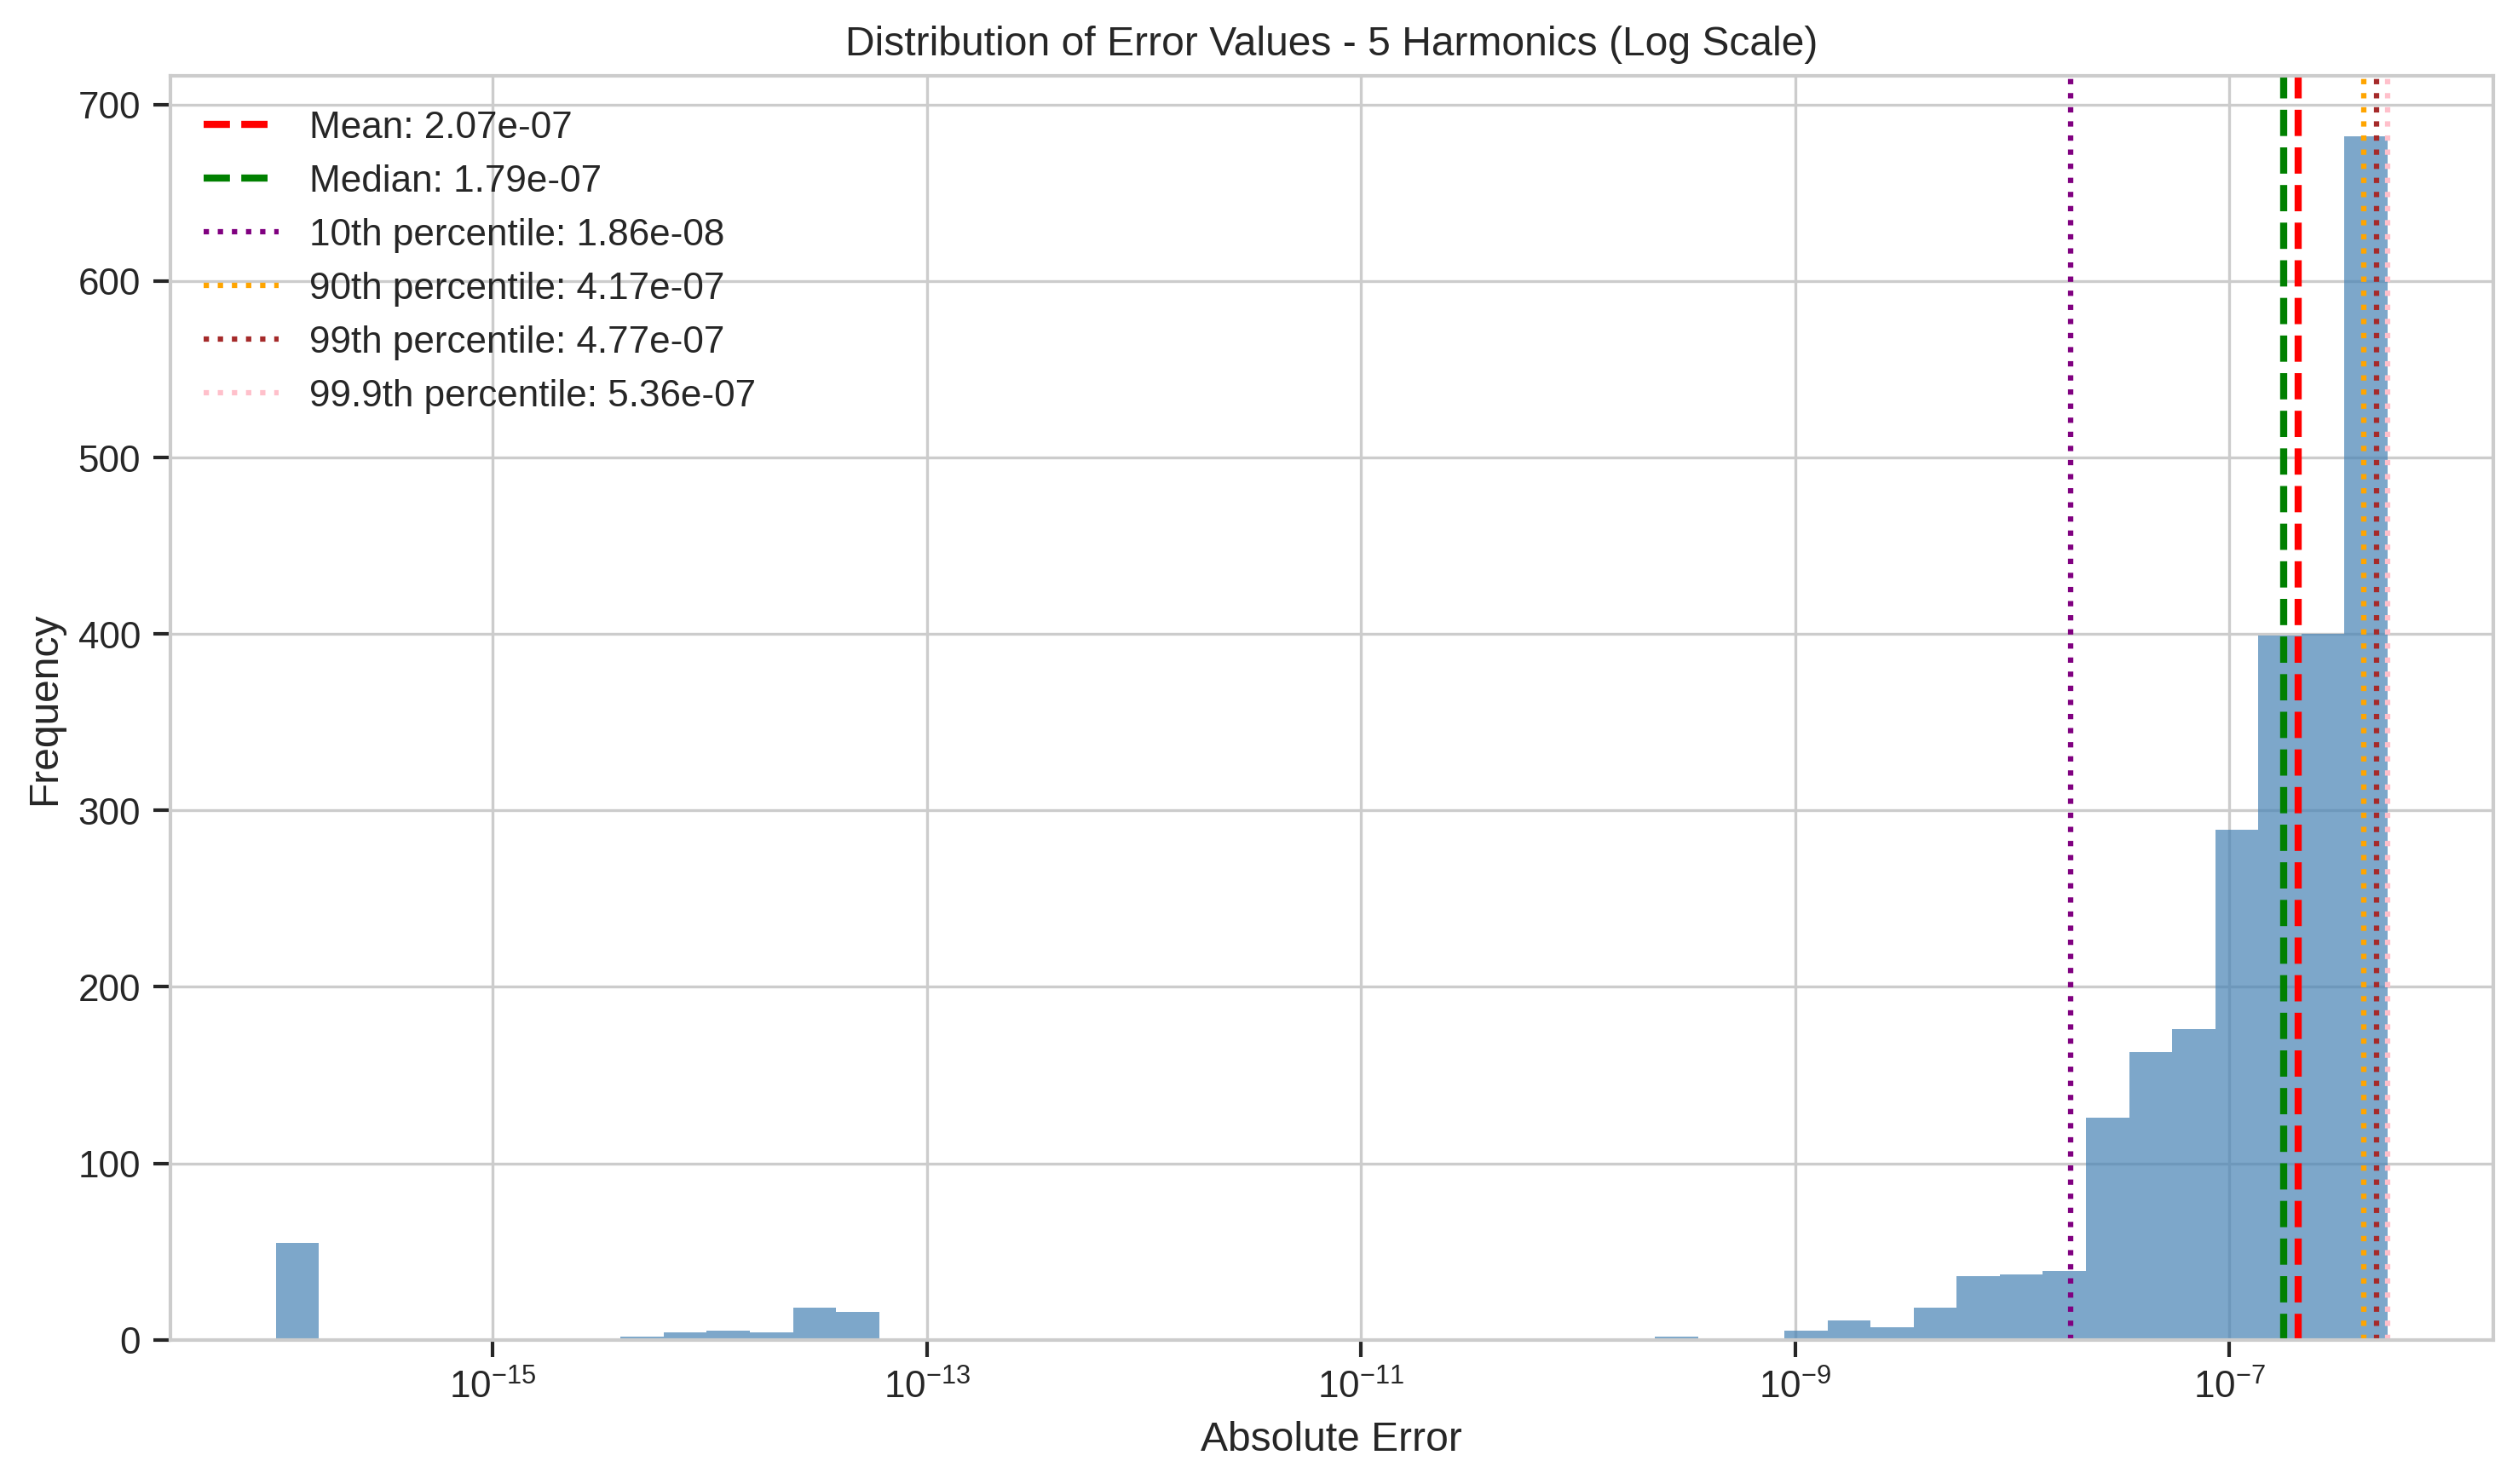
\includegraphics[width=0.9\linewidth]{figures/error_distribution_5h.png}
    \caption{Distribution of Absolute Error Values for 5 Harmonics on a Logarithmic Scale.}
    \label{fig:error_dist_5h}
\end{figure}

The 5-harmonic error distribution shows slightly elevated values compared to the 10-harmonic case, with a mean of \(2.07 \times 10^{-7}\) and a median of \(1.79 \times 10^{-7}\). The errors are still relatively low, with most values concentrated between \(10^{-8}\) and \(10^{-6}\), and a sharp drop-off beyond the 99.9th percentile at \(5.36 \times 10^{-7}\). The broader spread compared to the 10-harmonic model suggests reduced representational power due to fewer basis functions. While still highly accurate, the slight degradation implies that 5 harmonics may be insufficient for capturing finer signal components. Thus, increasing to 10 harmonics appears to yield a significant improvement in accuracy with only a modest increase in model complexity.

\begin{figure}[t]
    \centering
    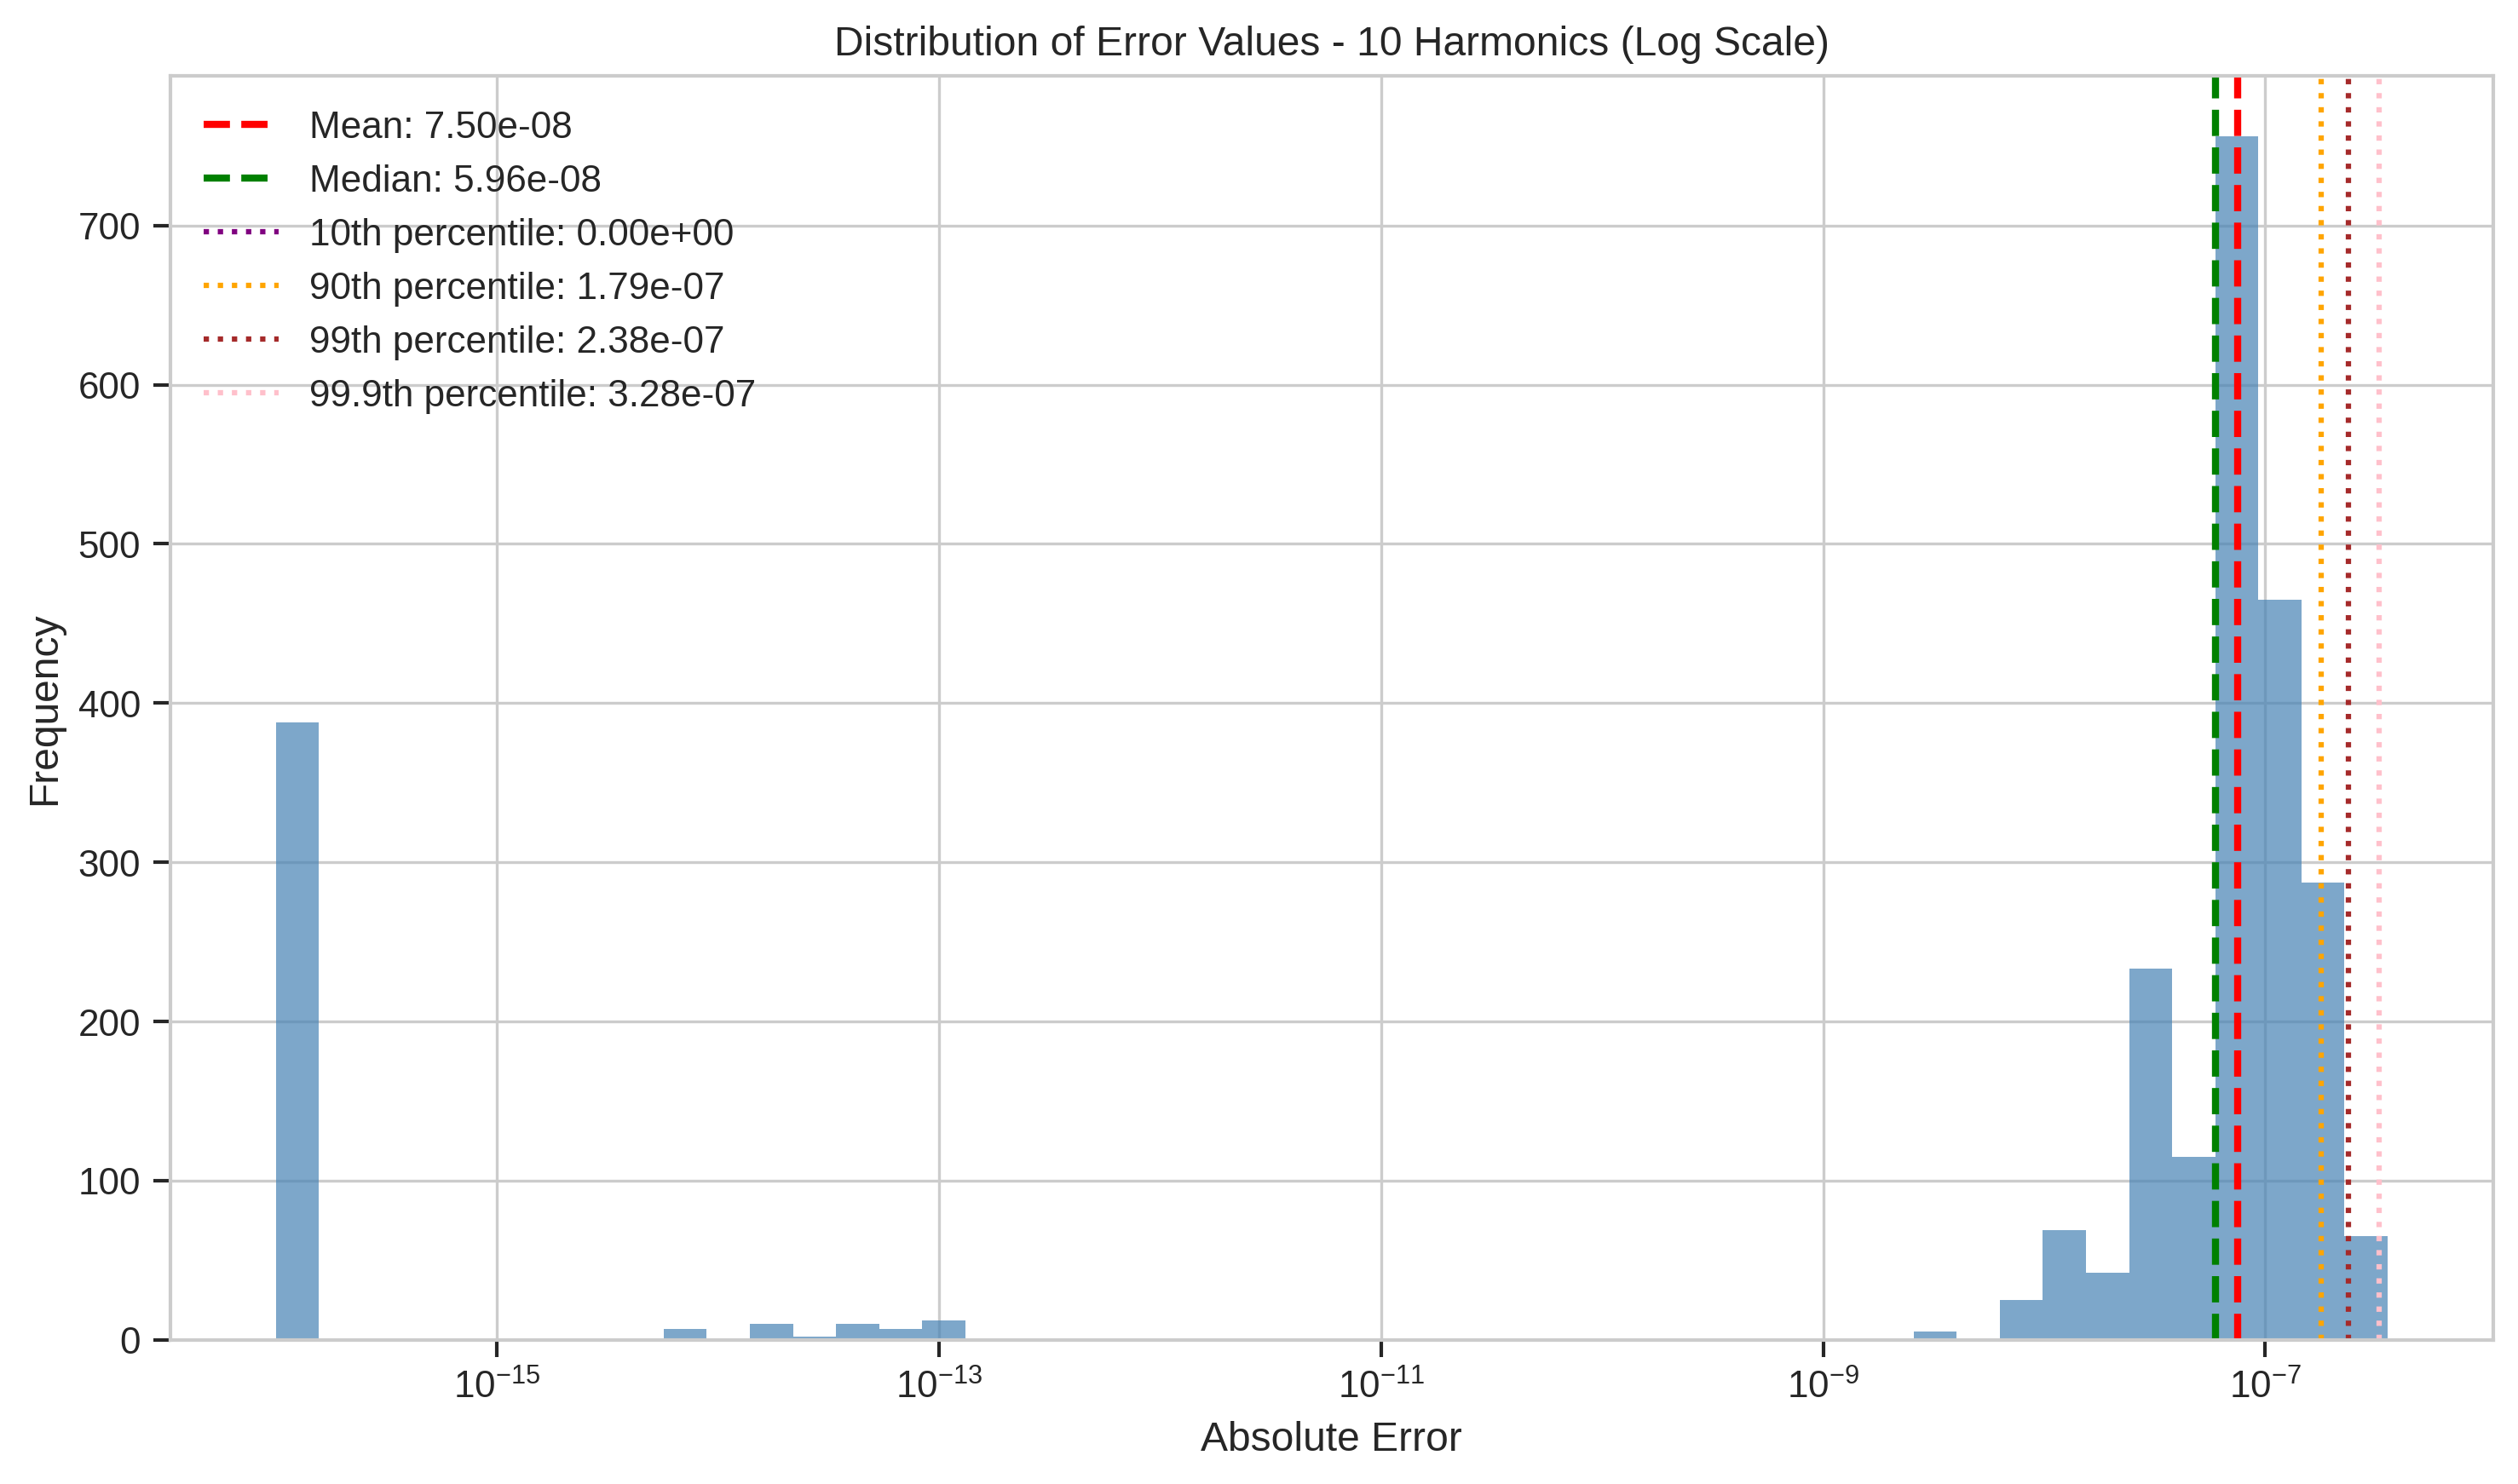
\includegraphics[width=0.9\linewidth]{figures/error_distribution_10h.png}
    \caption{Distribution of Absolute Error Values for 10 Harmonics on a Logarithmic Scale.}
    \label{fig:error_dist_10h}
\end{figure}

This figure presents the error distribution for the 10-harmonic configuration. The error values are significantly lower than in the 15-harmonic case, with a mean of \(7.50 \times 10^{-8}\) and a median of \(5.96 \times 10^{-8}\), suggesting highly accurate reconstruction. The tight clustering of percentiles—90th at \(1.79 \times 10^{-7}\), 99th at \(2.38 \times 10^{-7}\)—indicates low variance across the dataset. A large spike near machine precision around \(10^{-15}\) further confirms the system's high fidelity. This configuration strikes an effective balance between model complexity and accuracy, achieving minimal error without introducing excessive harmonics. It likely represents the optimal harmonic count for this specific reconstruction task.

\begin{figure}[t]
    \centering
    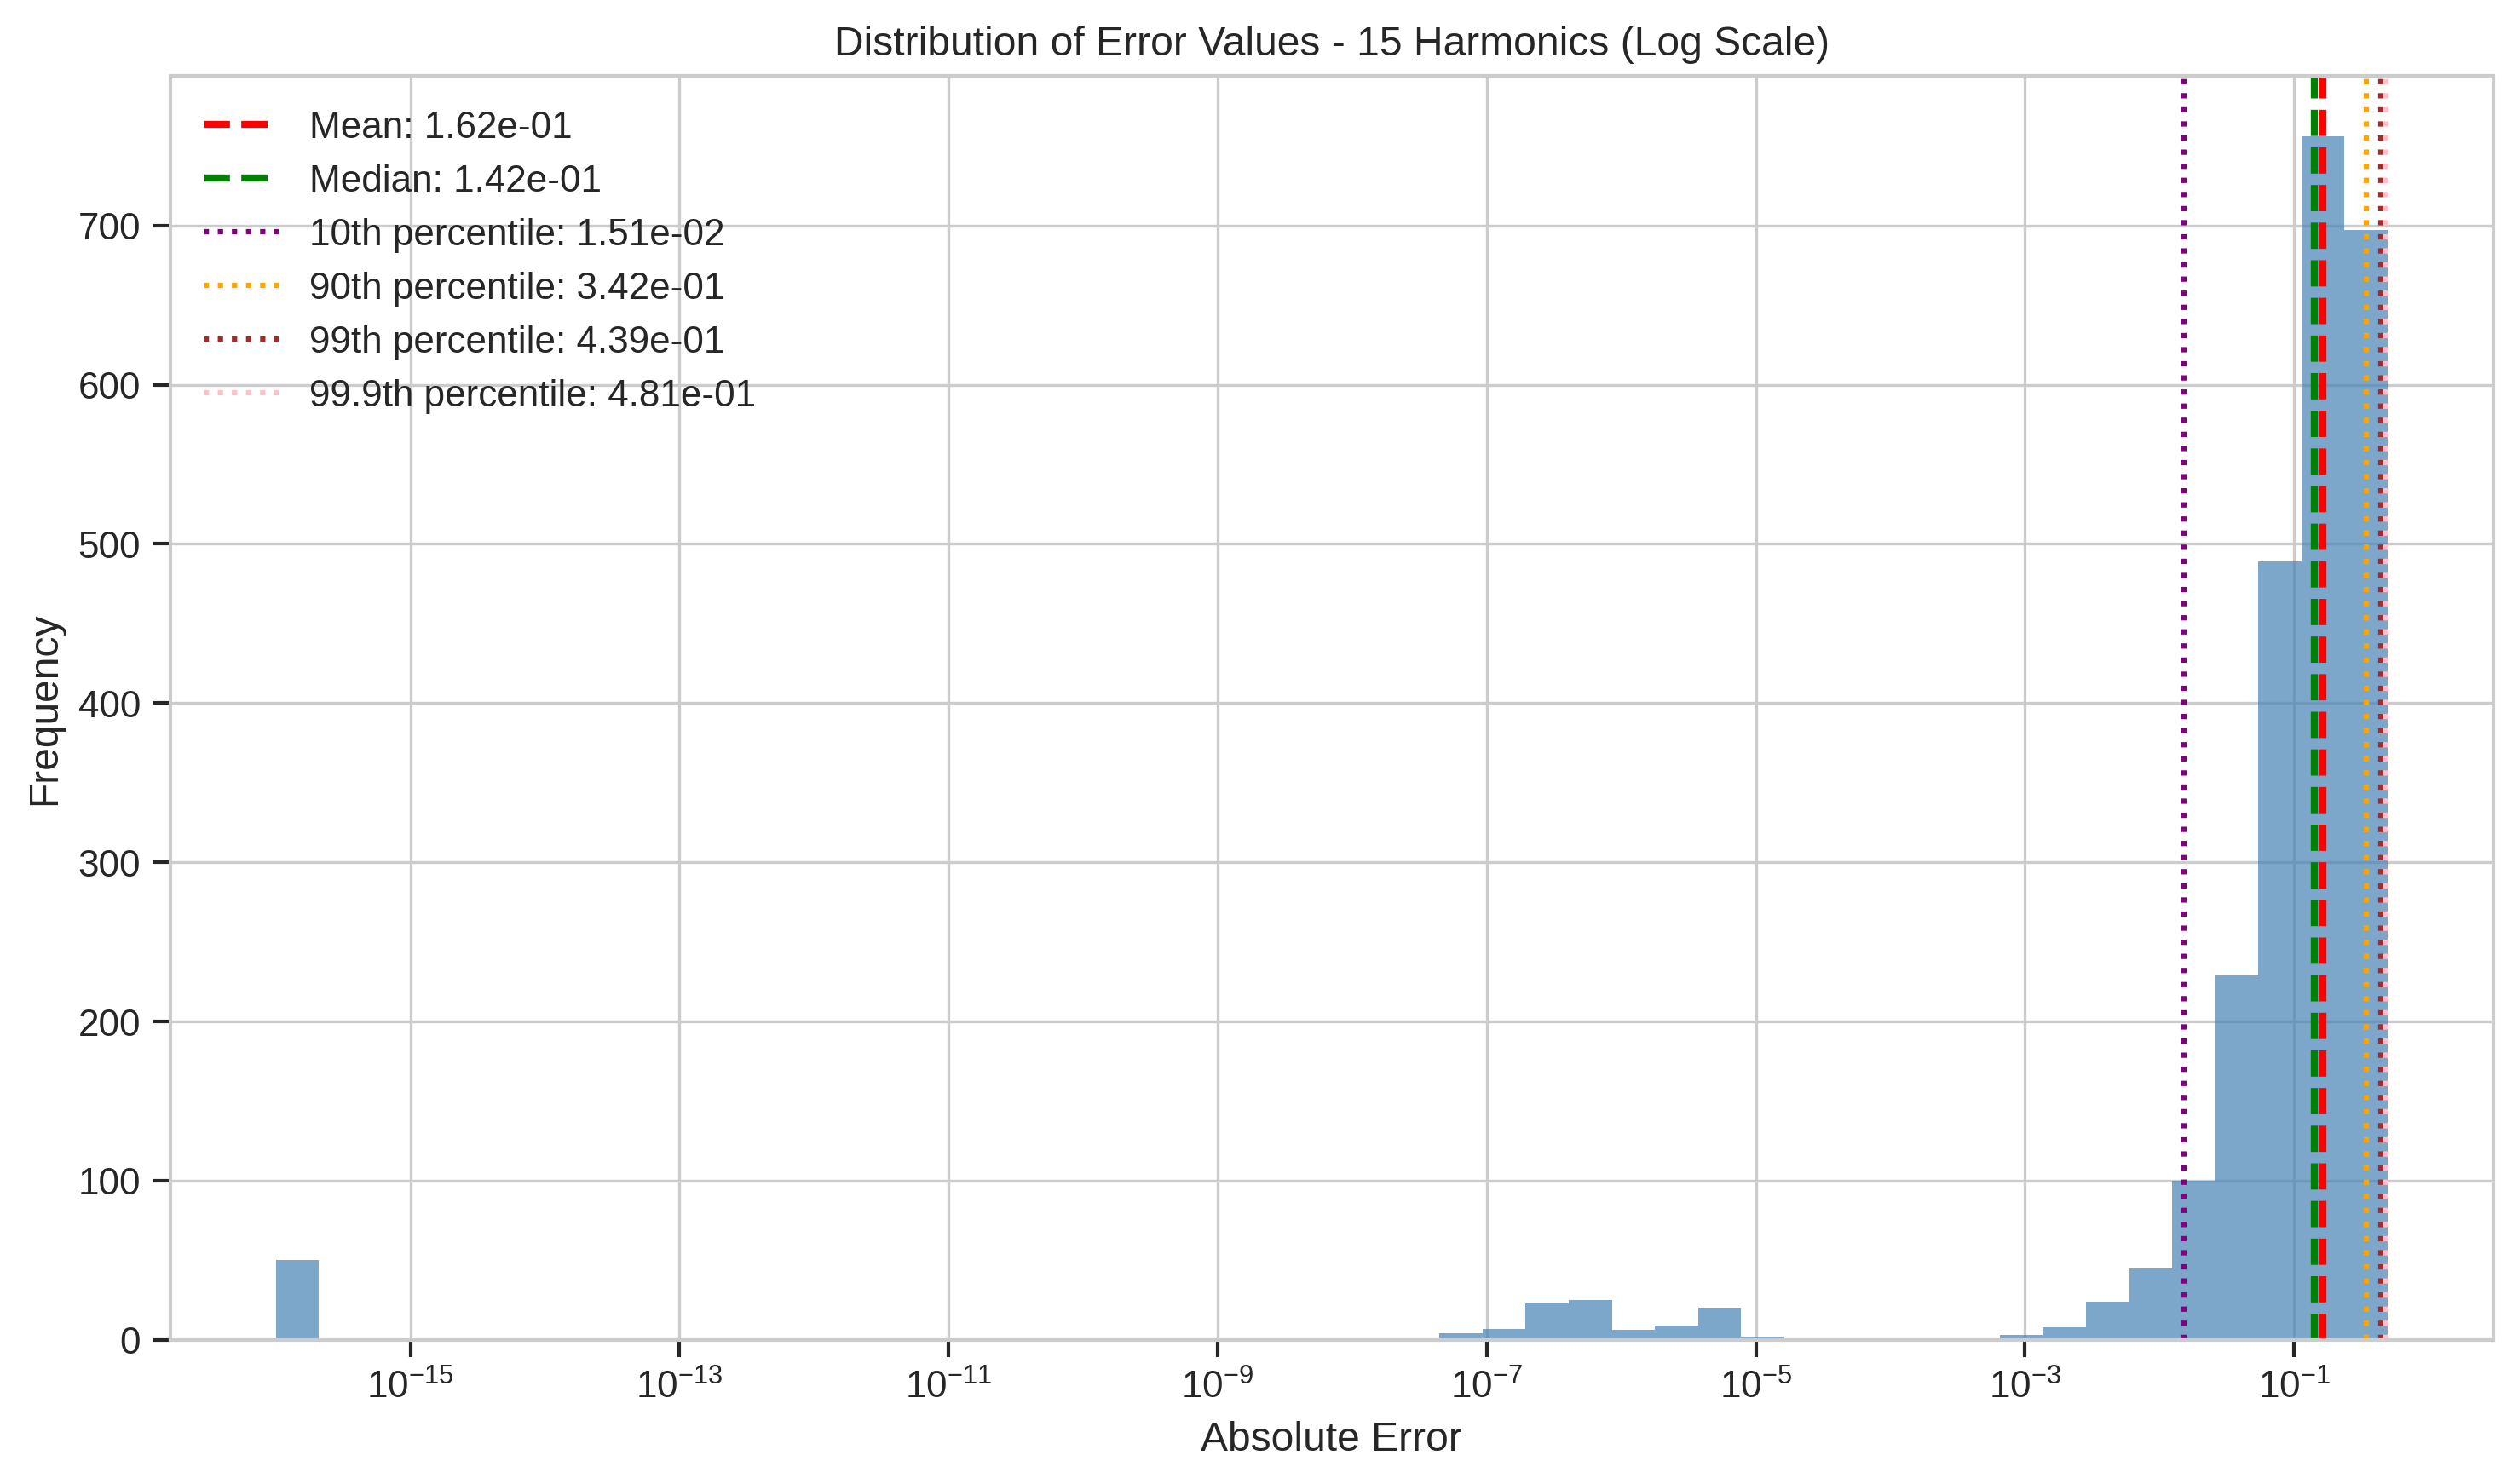
\includegraphics[width=0.9\linewidth]{figures/error_distribution_15h.png}
    \caption{Distribution of Absolute Error Values for 15 Harmonics on a Logarithmic Scale.}
    \label{fig:error_dist_15h}
\end{figure}

The histogram shows the absolute error distribution for the 15-harmonic reconstruction. The errors are concentrated in the range of \(10^{-2}\) to \(10^0\), with a mean error of \(1.62 \times 10^{-1}\) and a median of \(1.42 \times 10^{-1}\), indicating a right-skewed distribution. Notably, the 10th percentile error is \(1.51 \times 10^{-2}\), while the 99.9th percentile reaches \(4.81 \times 10^{-1}\), revealing a substantial spread in error magnitudes. Compared to lower harmonic counts, this configuration shows higher overall error, suggesting that increasing the harmonic count beyond a certain point may not improve and may even degrade accuracy due to overfitting or numerical instability. This emphasizes the need for harmonic number optimization in error-sensitive applications.

\begin{figure}[t]
    \centering
    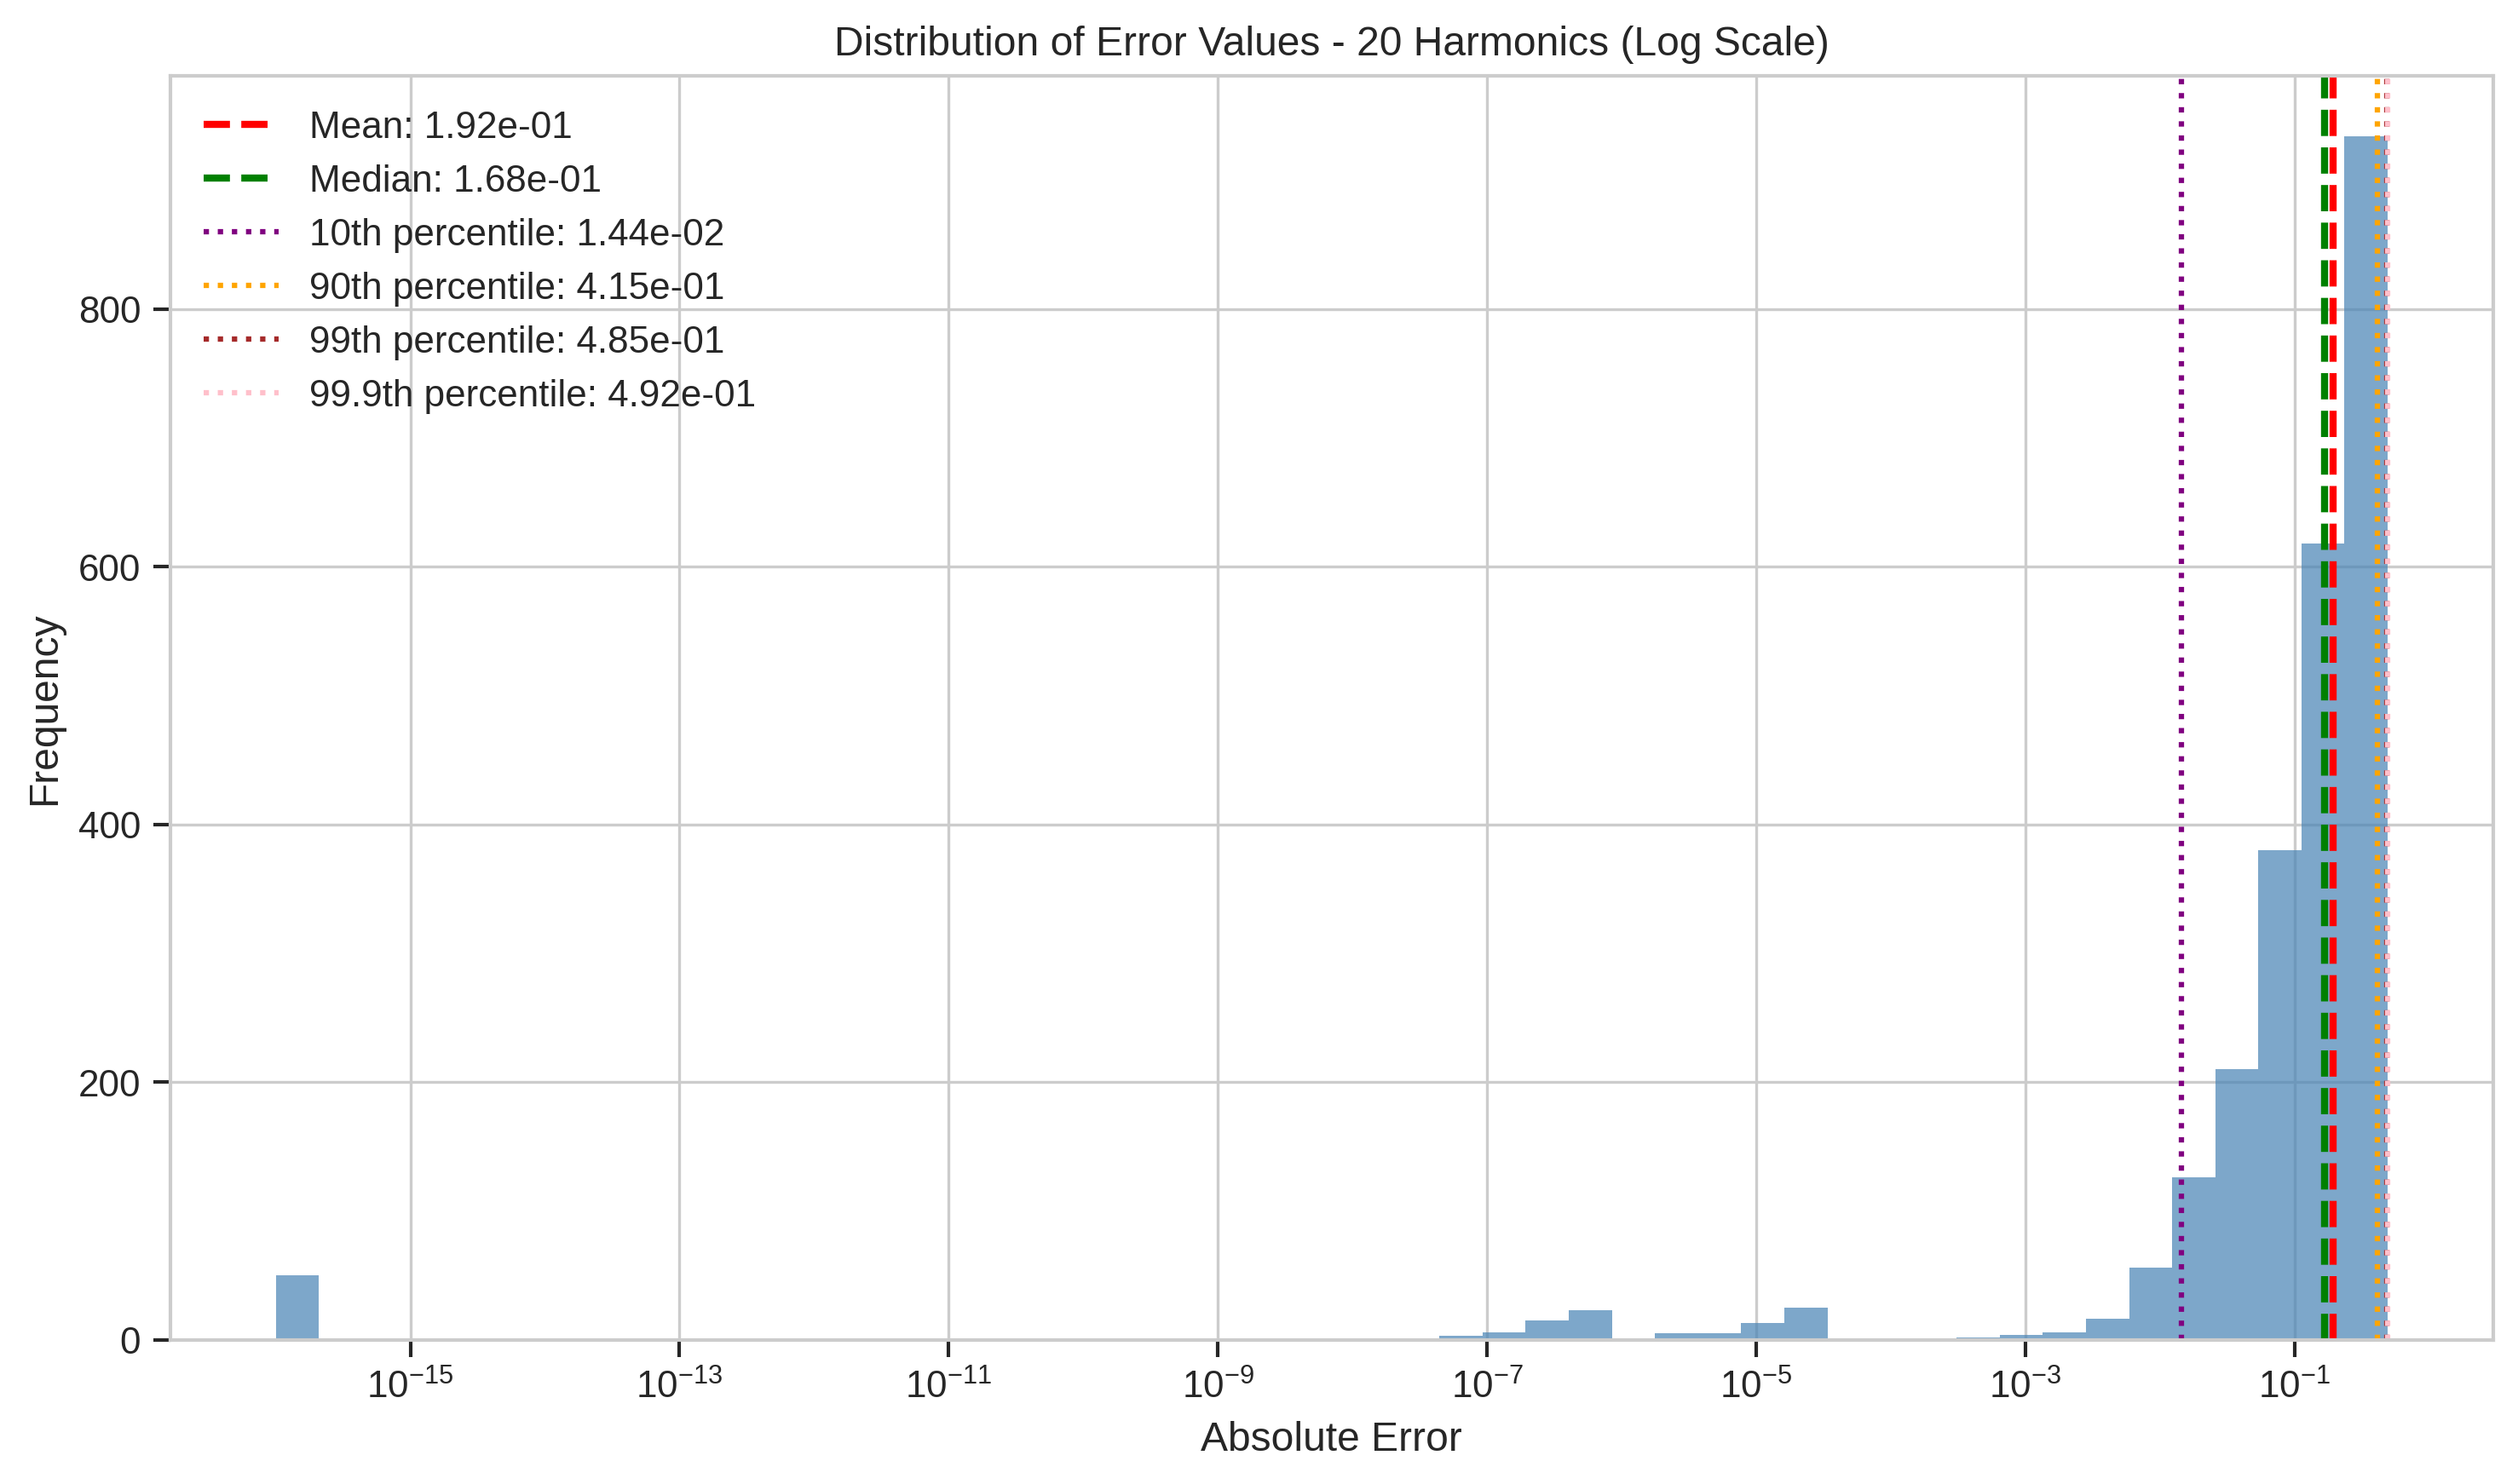
\includegraphics[width=0.9\linewidth]{figures/error_distribution_20h.png}
    \caption{Error distribution for 20 harmonics.}
    \label{fig:error_20h}
\end{figure}

At 20 harmonics, the error distribution reveals a mean of 0.192 and a median of 0.168, comparable to the 25-harmonic result. The 10th percentile sits at 0.0144, higher than in the 30+ harmonic models, suggesting a slight decline in minimum error performance. While still tightly concentrated, the histogram shows a slight increase in spread compared to higher-order models. The 90th and 99.9th percentiles hover around 0.415 and 0.492, respectively. This figure indicates a slight performance degradation as harmonic resolution decreases but not dramatically so. The 20-harmonic model may be ideal for real-time or embedded applications where computational resources are limited, offering a strong balance between error magnitude and efficiency.

\begin{figure}[t]
    \centering
    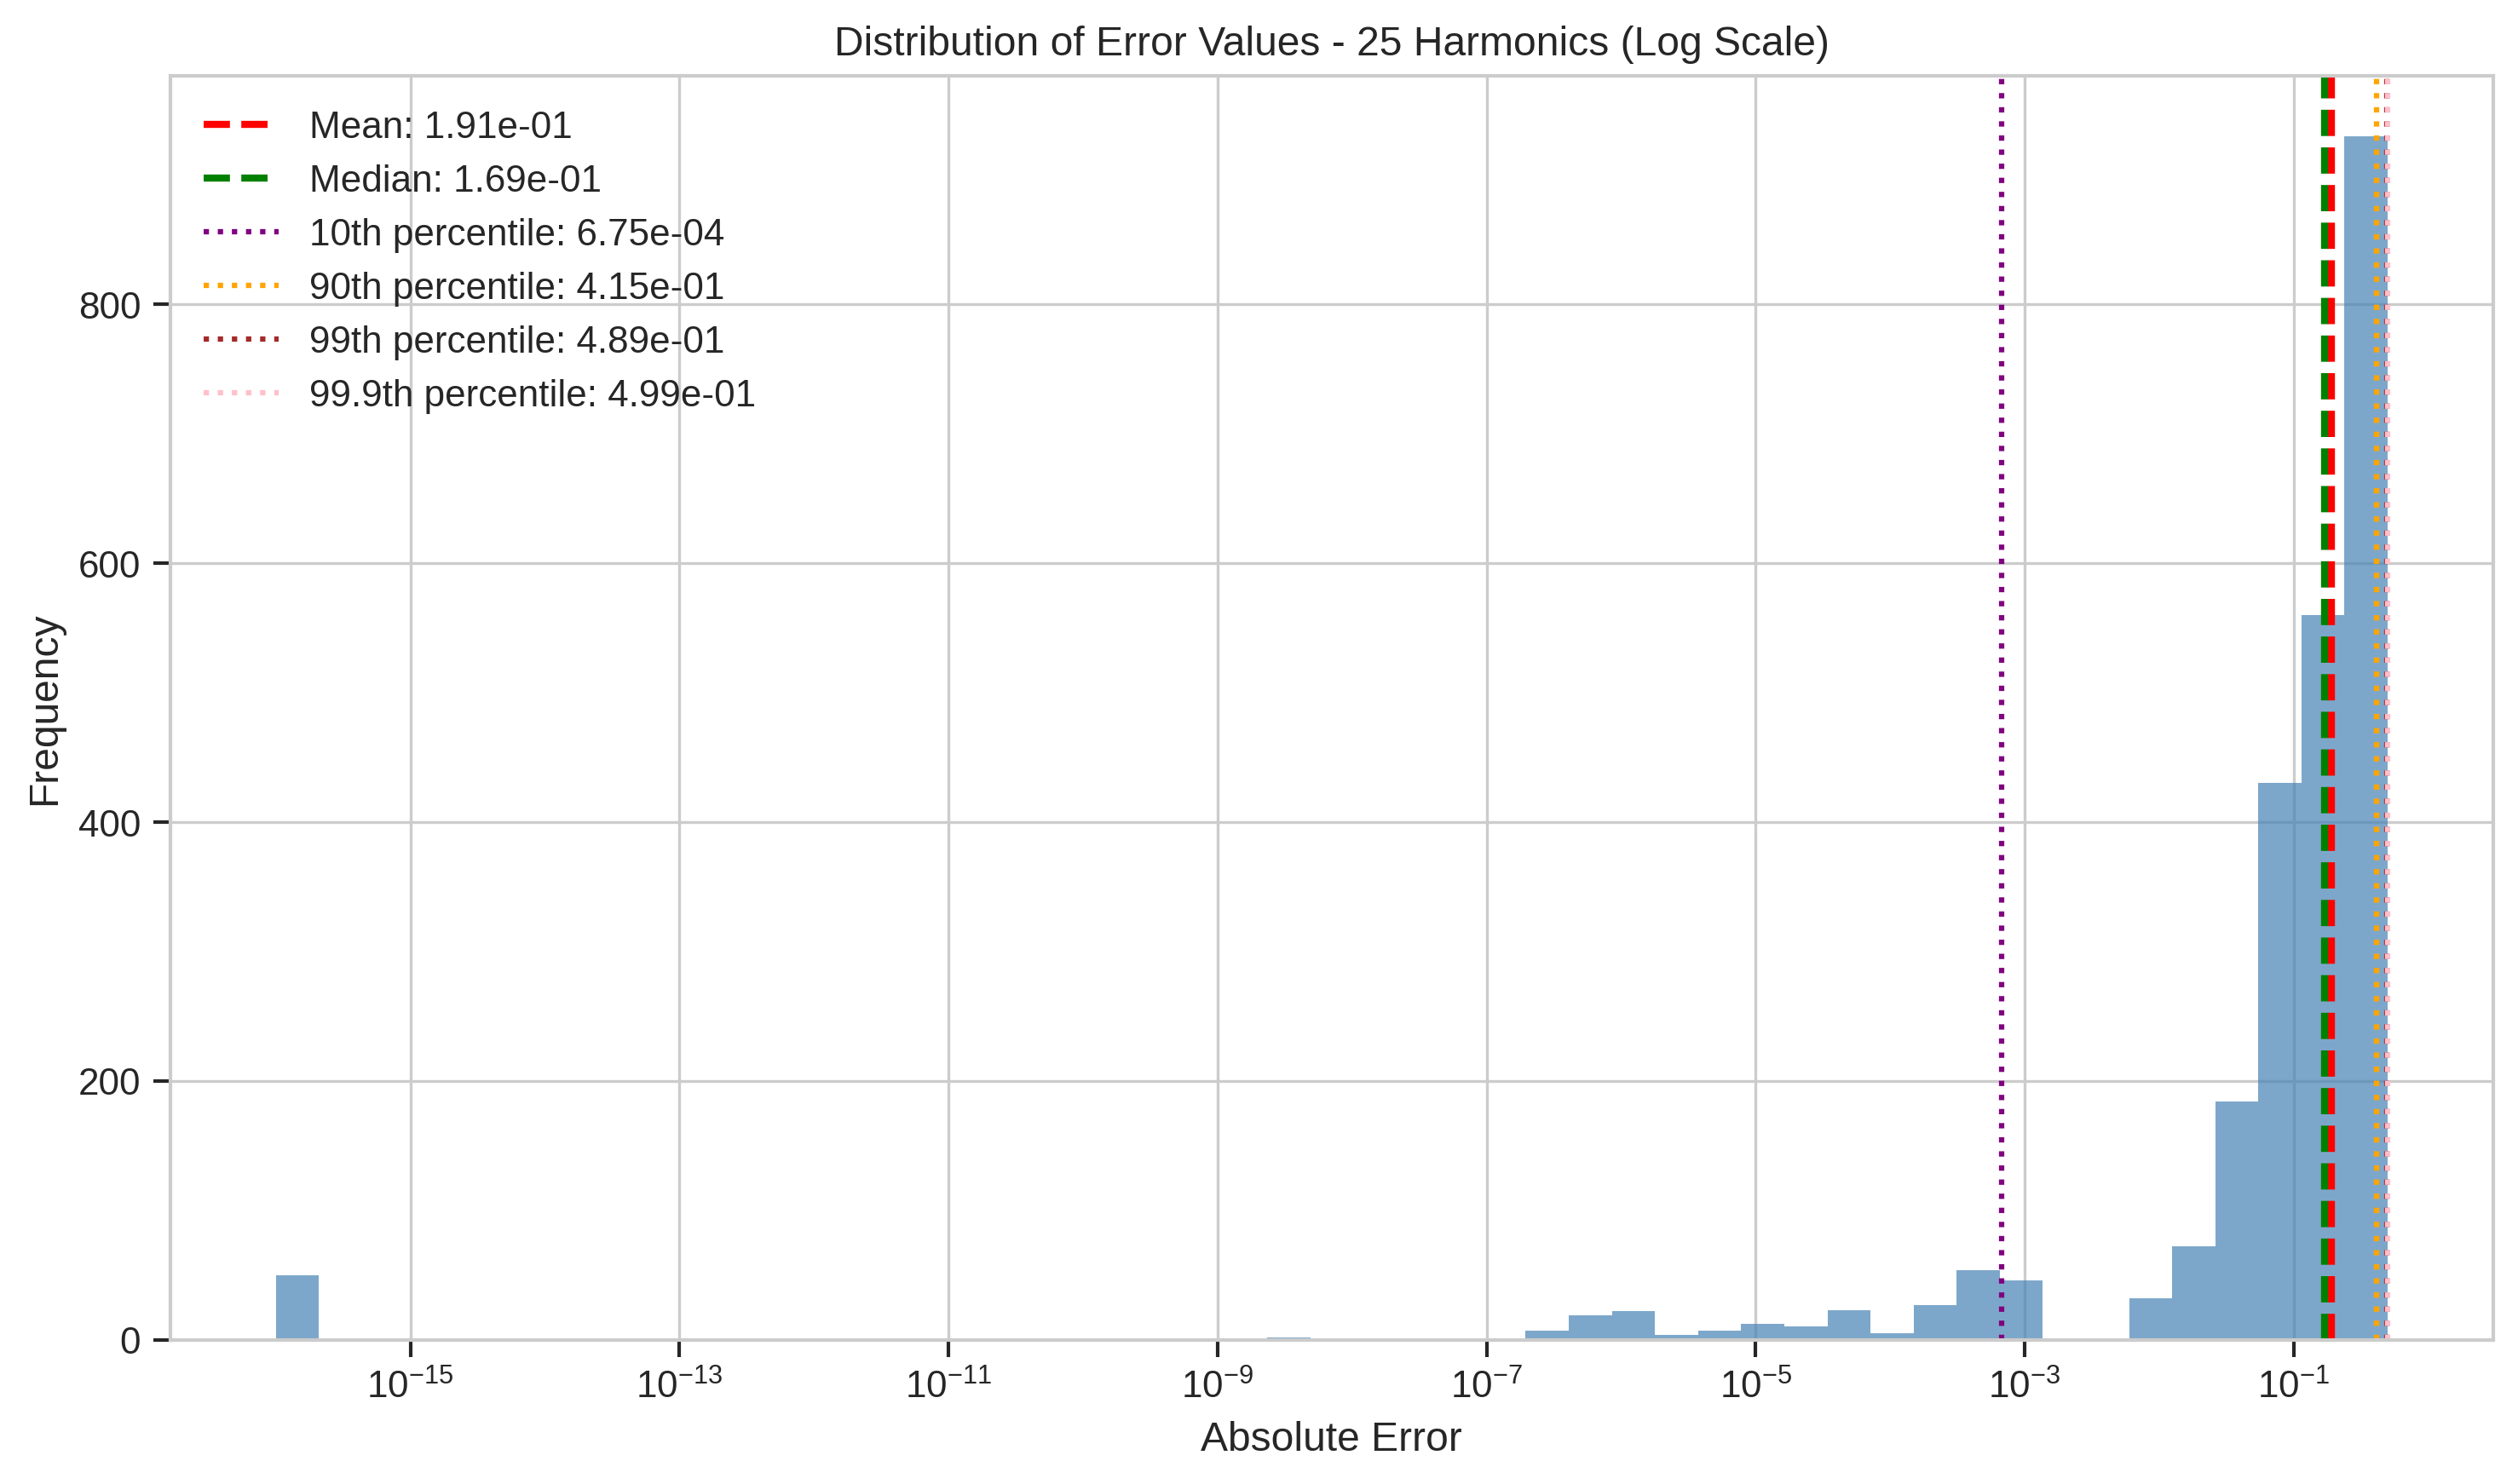
\includegraphics[width=0.9\linewidth]{figures/error_distribution_25h.png}
    \caption{Error distribution for 25 harmonics.}
    \label{fig:error_25h}
\end{figure}

The 25-harmonic configuration yields a mean absolute error of 0.191 and a median of 0.169. Unlike the higher harmonic cases, the 10th percentile is notably higher at 6.75e-4, indicating that fewer reconstructions achieve extremely low errors. Nevertheless, the distribution remains highly peaked, with the majority of samples falling between \(10^{-2}\) and \(10^{0}\). The 90th, 99th, and 99.9th percentiles remain consistent at around 0.415, 0.489, and 0.499, respectively. This indicates that while accuracy is slightly reduced compared to the 30+ harmonic models, the trade-off may be acceptable in scenarios prioritizing computational speed or memory efficiency. The 25-harmonic model thus represents a balanced compromise for moderately constrained applications.

\begin{figure}[t]
    \centering
    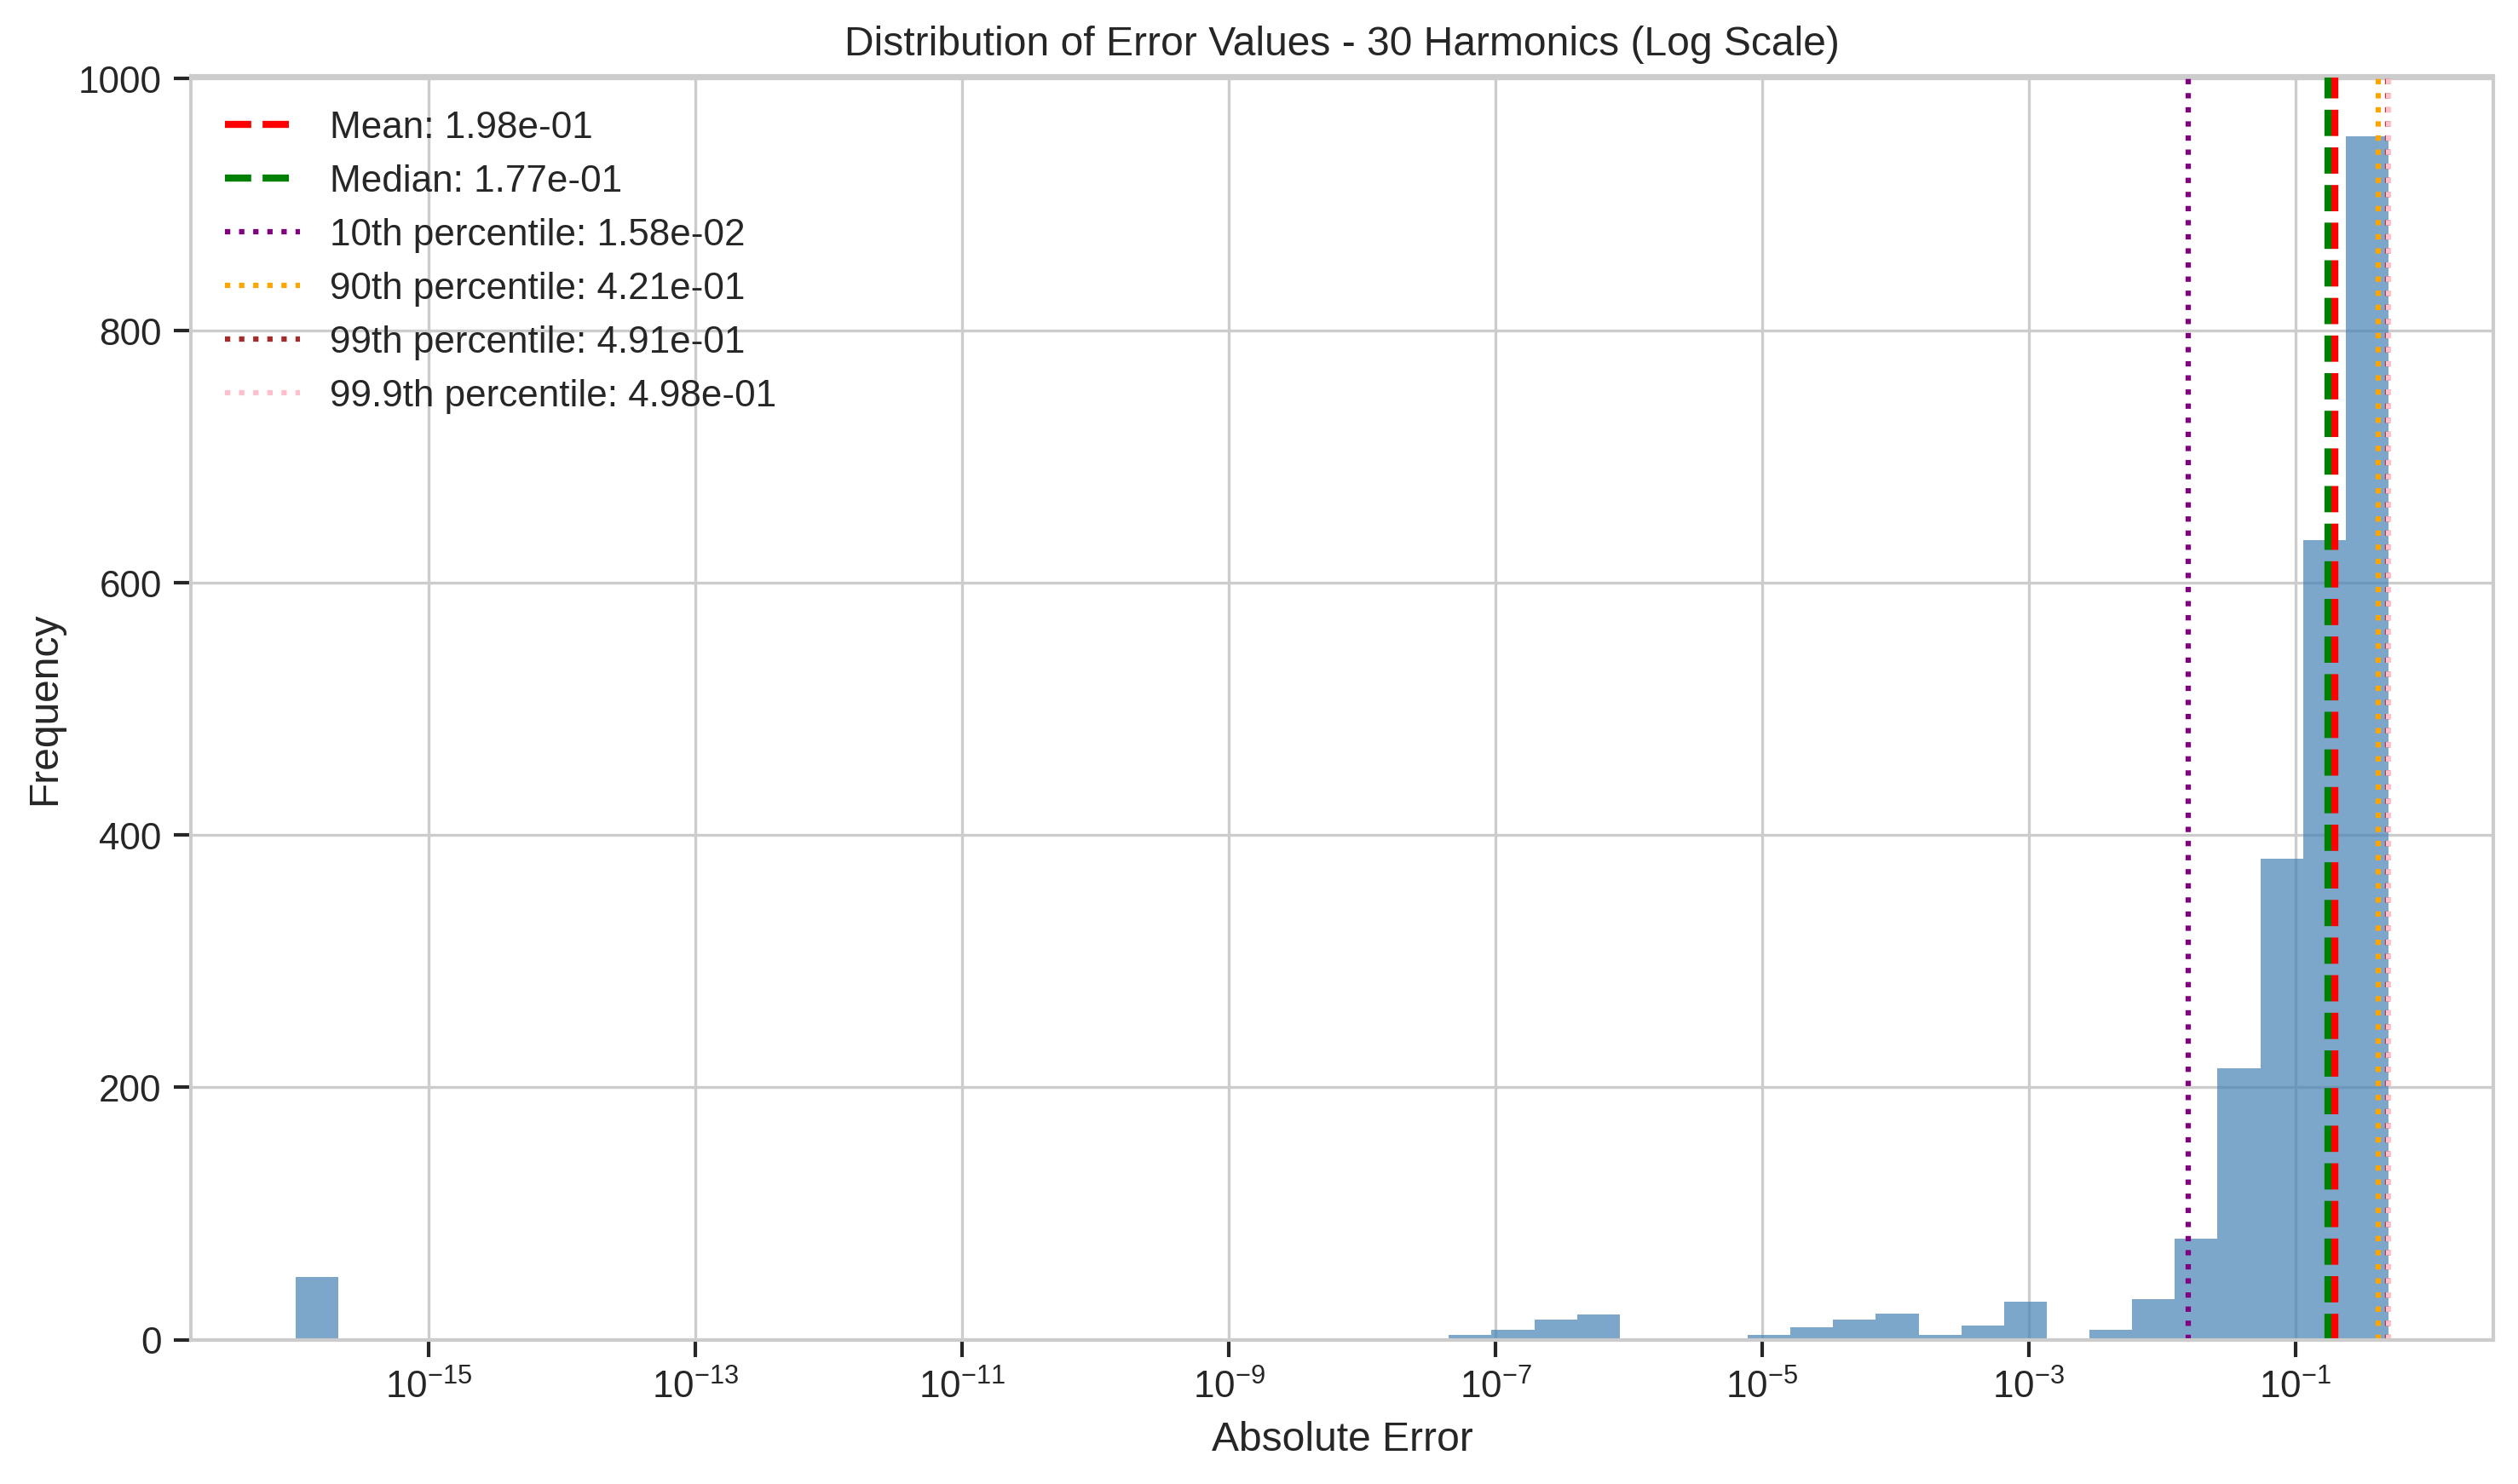
\includegraphics[width=0.9\linewidth]{figures/error_distribution_30h.png}
    \caption{Error distribution for 30 harmonics.}
    \label{fig:error_30h}
\end{figure}

For 30 harmonics, the error distribution remains consistent with that of 35 and 40 harmonics. The mean error is 0.198 and the median is 0.177, showing a slightly higher central tendency. Despite a minor increase in central error statistics, the overall shape of the histogram is nearly identical, with error values concentrated in the \(10^{-2}\) to \(10^{0}\) range. The 10th percentile sits at 0.0158, while the 99.9th percentile approaches 0.498. These figures suggest that the model still captures the core signal characteristics effectively. However, the plateauing improvement in reconstruction performance indicates that models with more than 30 harmonics may offer limited gains for significantly higher complexity. Thus, 30 harmonics may serve as a practical cutoff point for achieving efficient yet accurate approximations.

\begin{figure}[t]
    \centering
    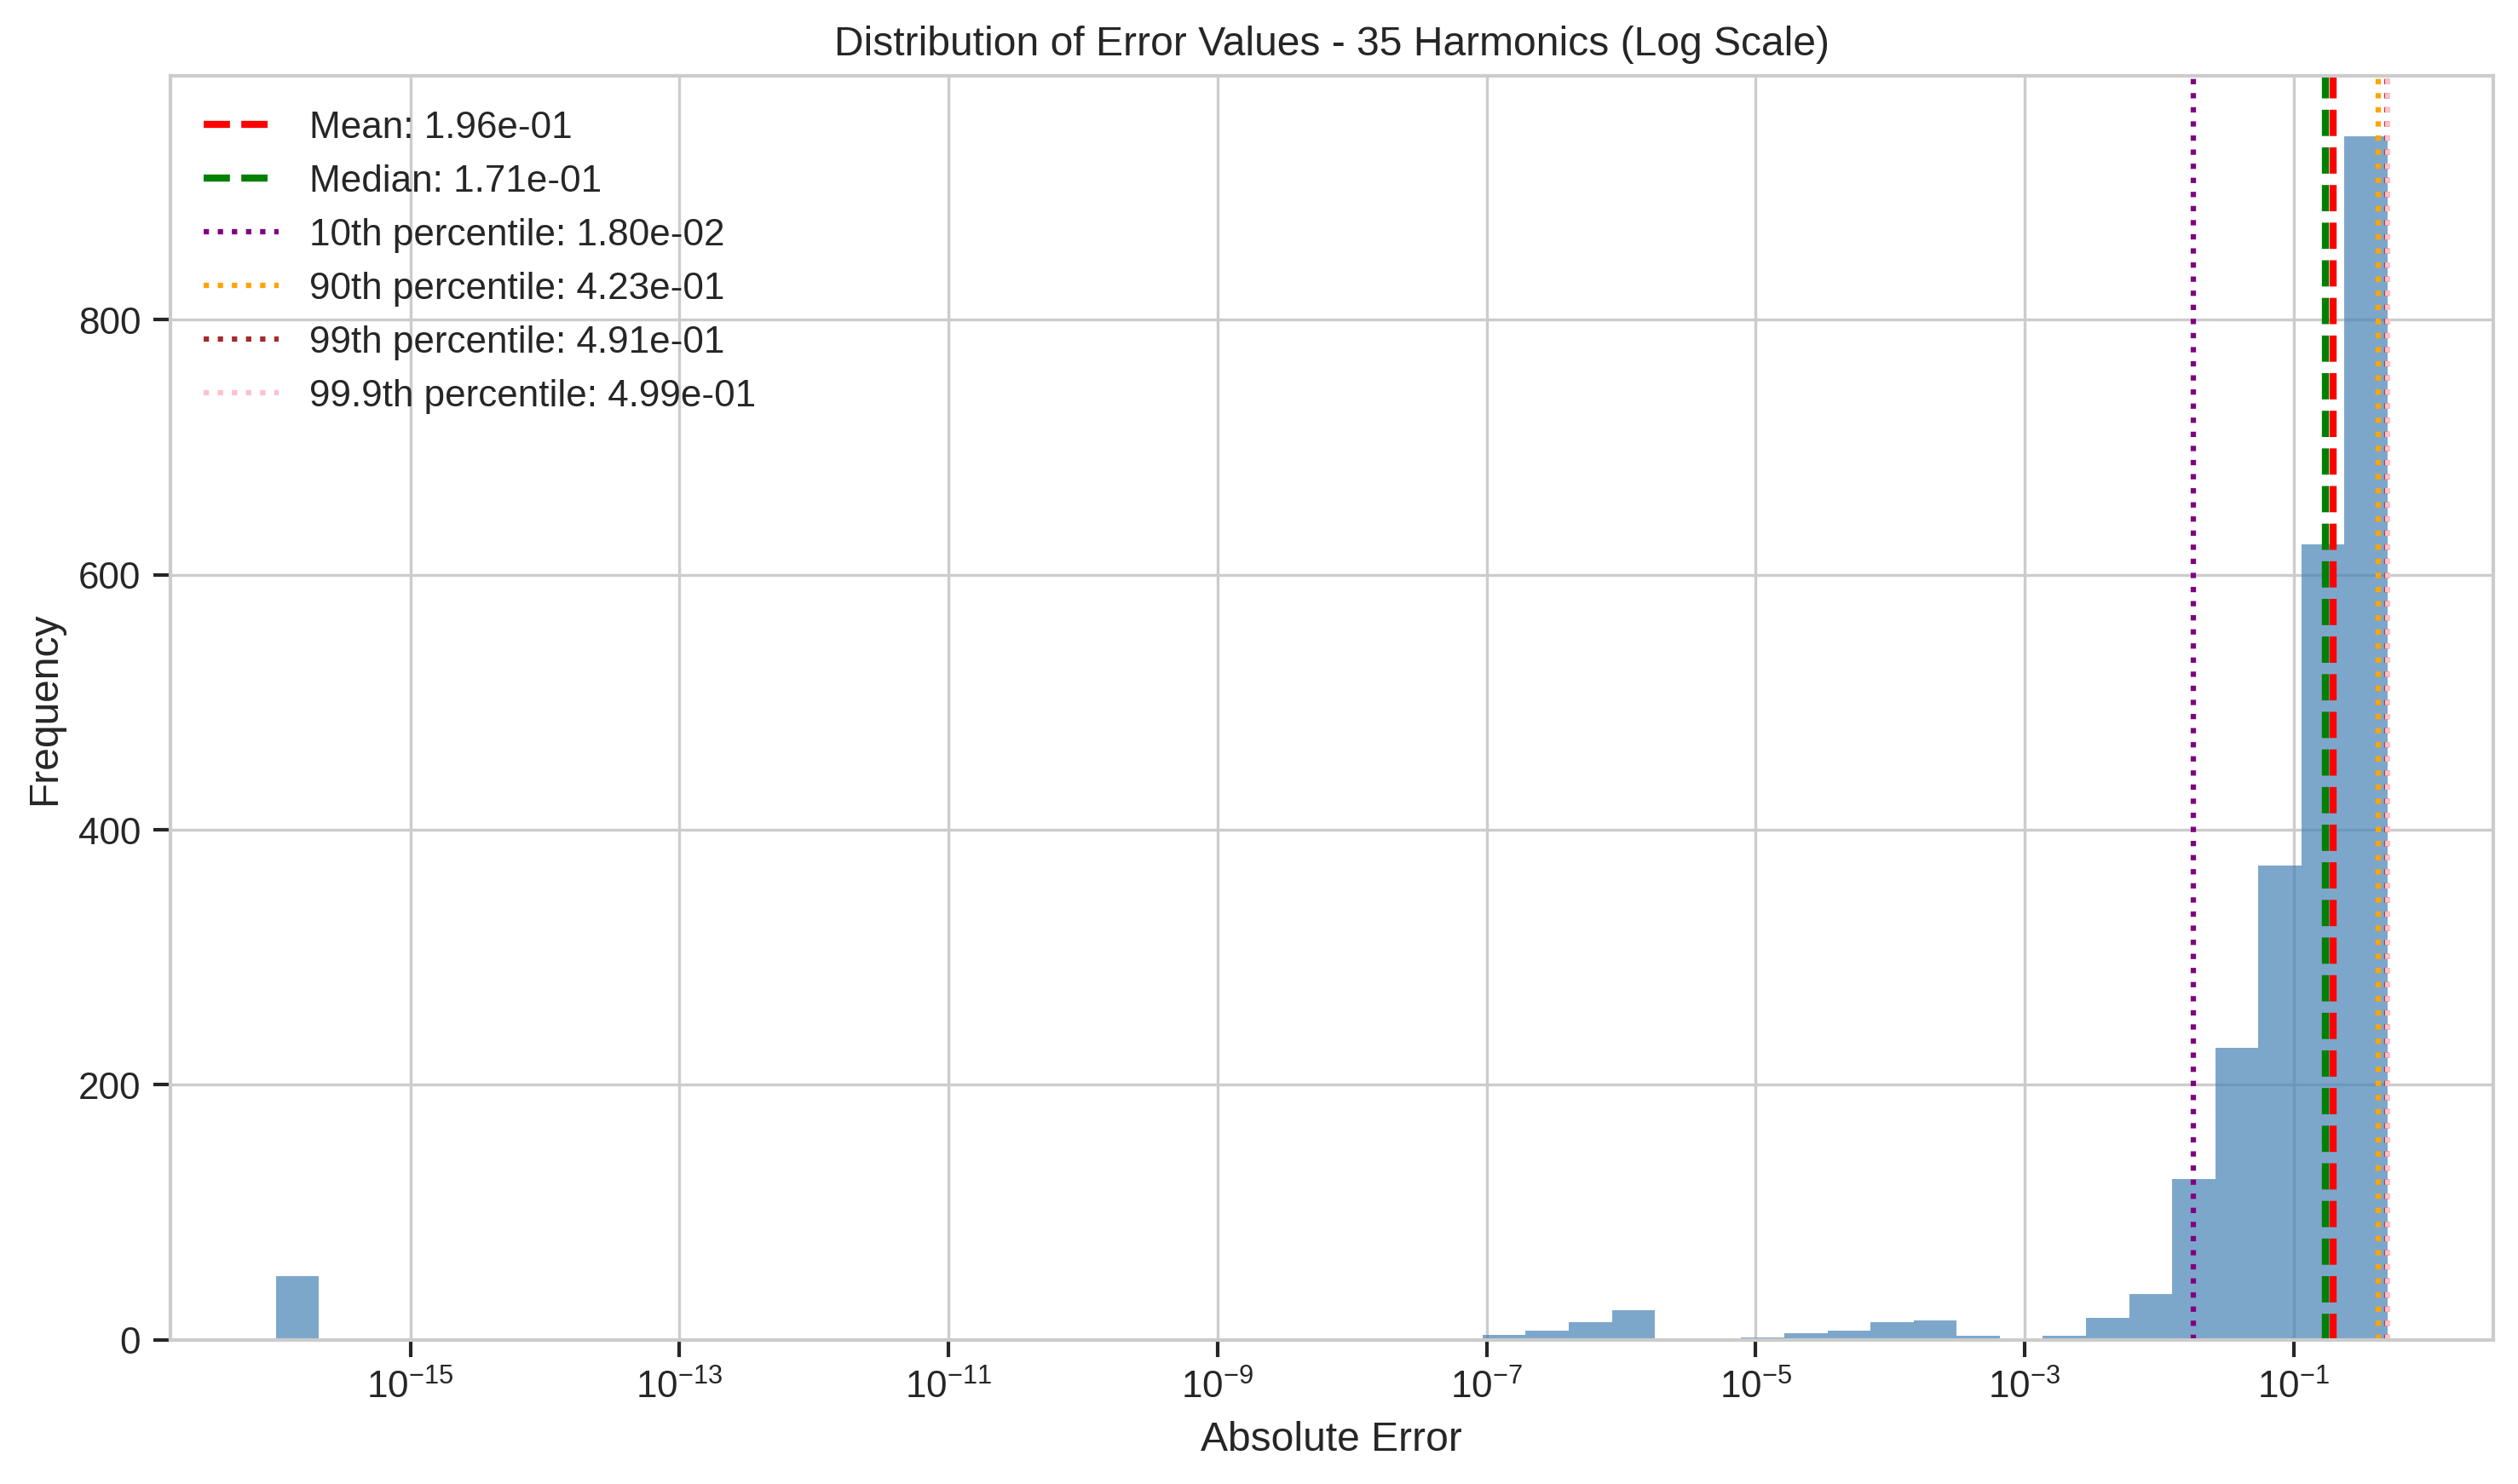
\includegraphics[width=0.9\linewidth]{figures/error_distribution_35h.png}
    \caption{Error distribution for 35 harmonics.}
    \label{fig:error_35h}
\end{figure}

The 35-harmonic model presents a tightly clustered error distribution with a mean error of 0.196 and a median of 0.171. The error values predominantly fall between \(10^{-2}\) and \(10^{0}\), similar to the 40-harmonic case. While the average error is slightly higher than that of the 40-harmonic model, the difference is marginal, highlighting that increasing harmonics may not linearly enhance accuracy. The 90th percentile reaches 0.423 and the 99.9th percentile nearly maxes out at 0.499. These statistics imply a consistent performance across most samples but with some high-error outliers. Overall, the 35-harmonic configuration offers an efficient trade-off between computational overhead and reconstruction fidelity, delivering performance comparable to the 40-harmonic case but with fewer basis components.

\begin{figure}[t]
    \centering
    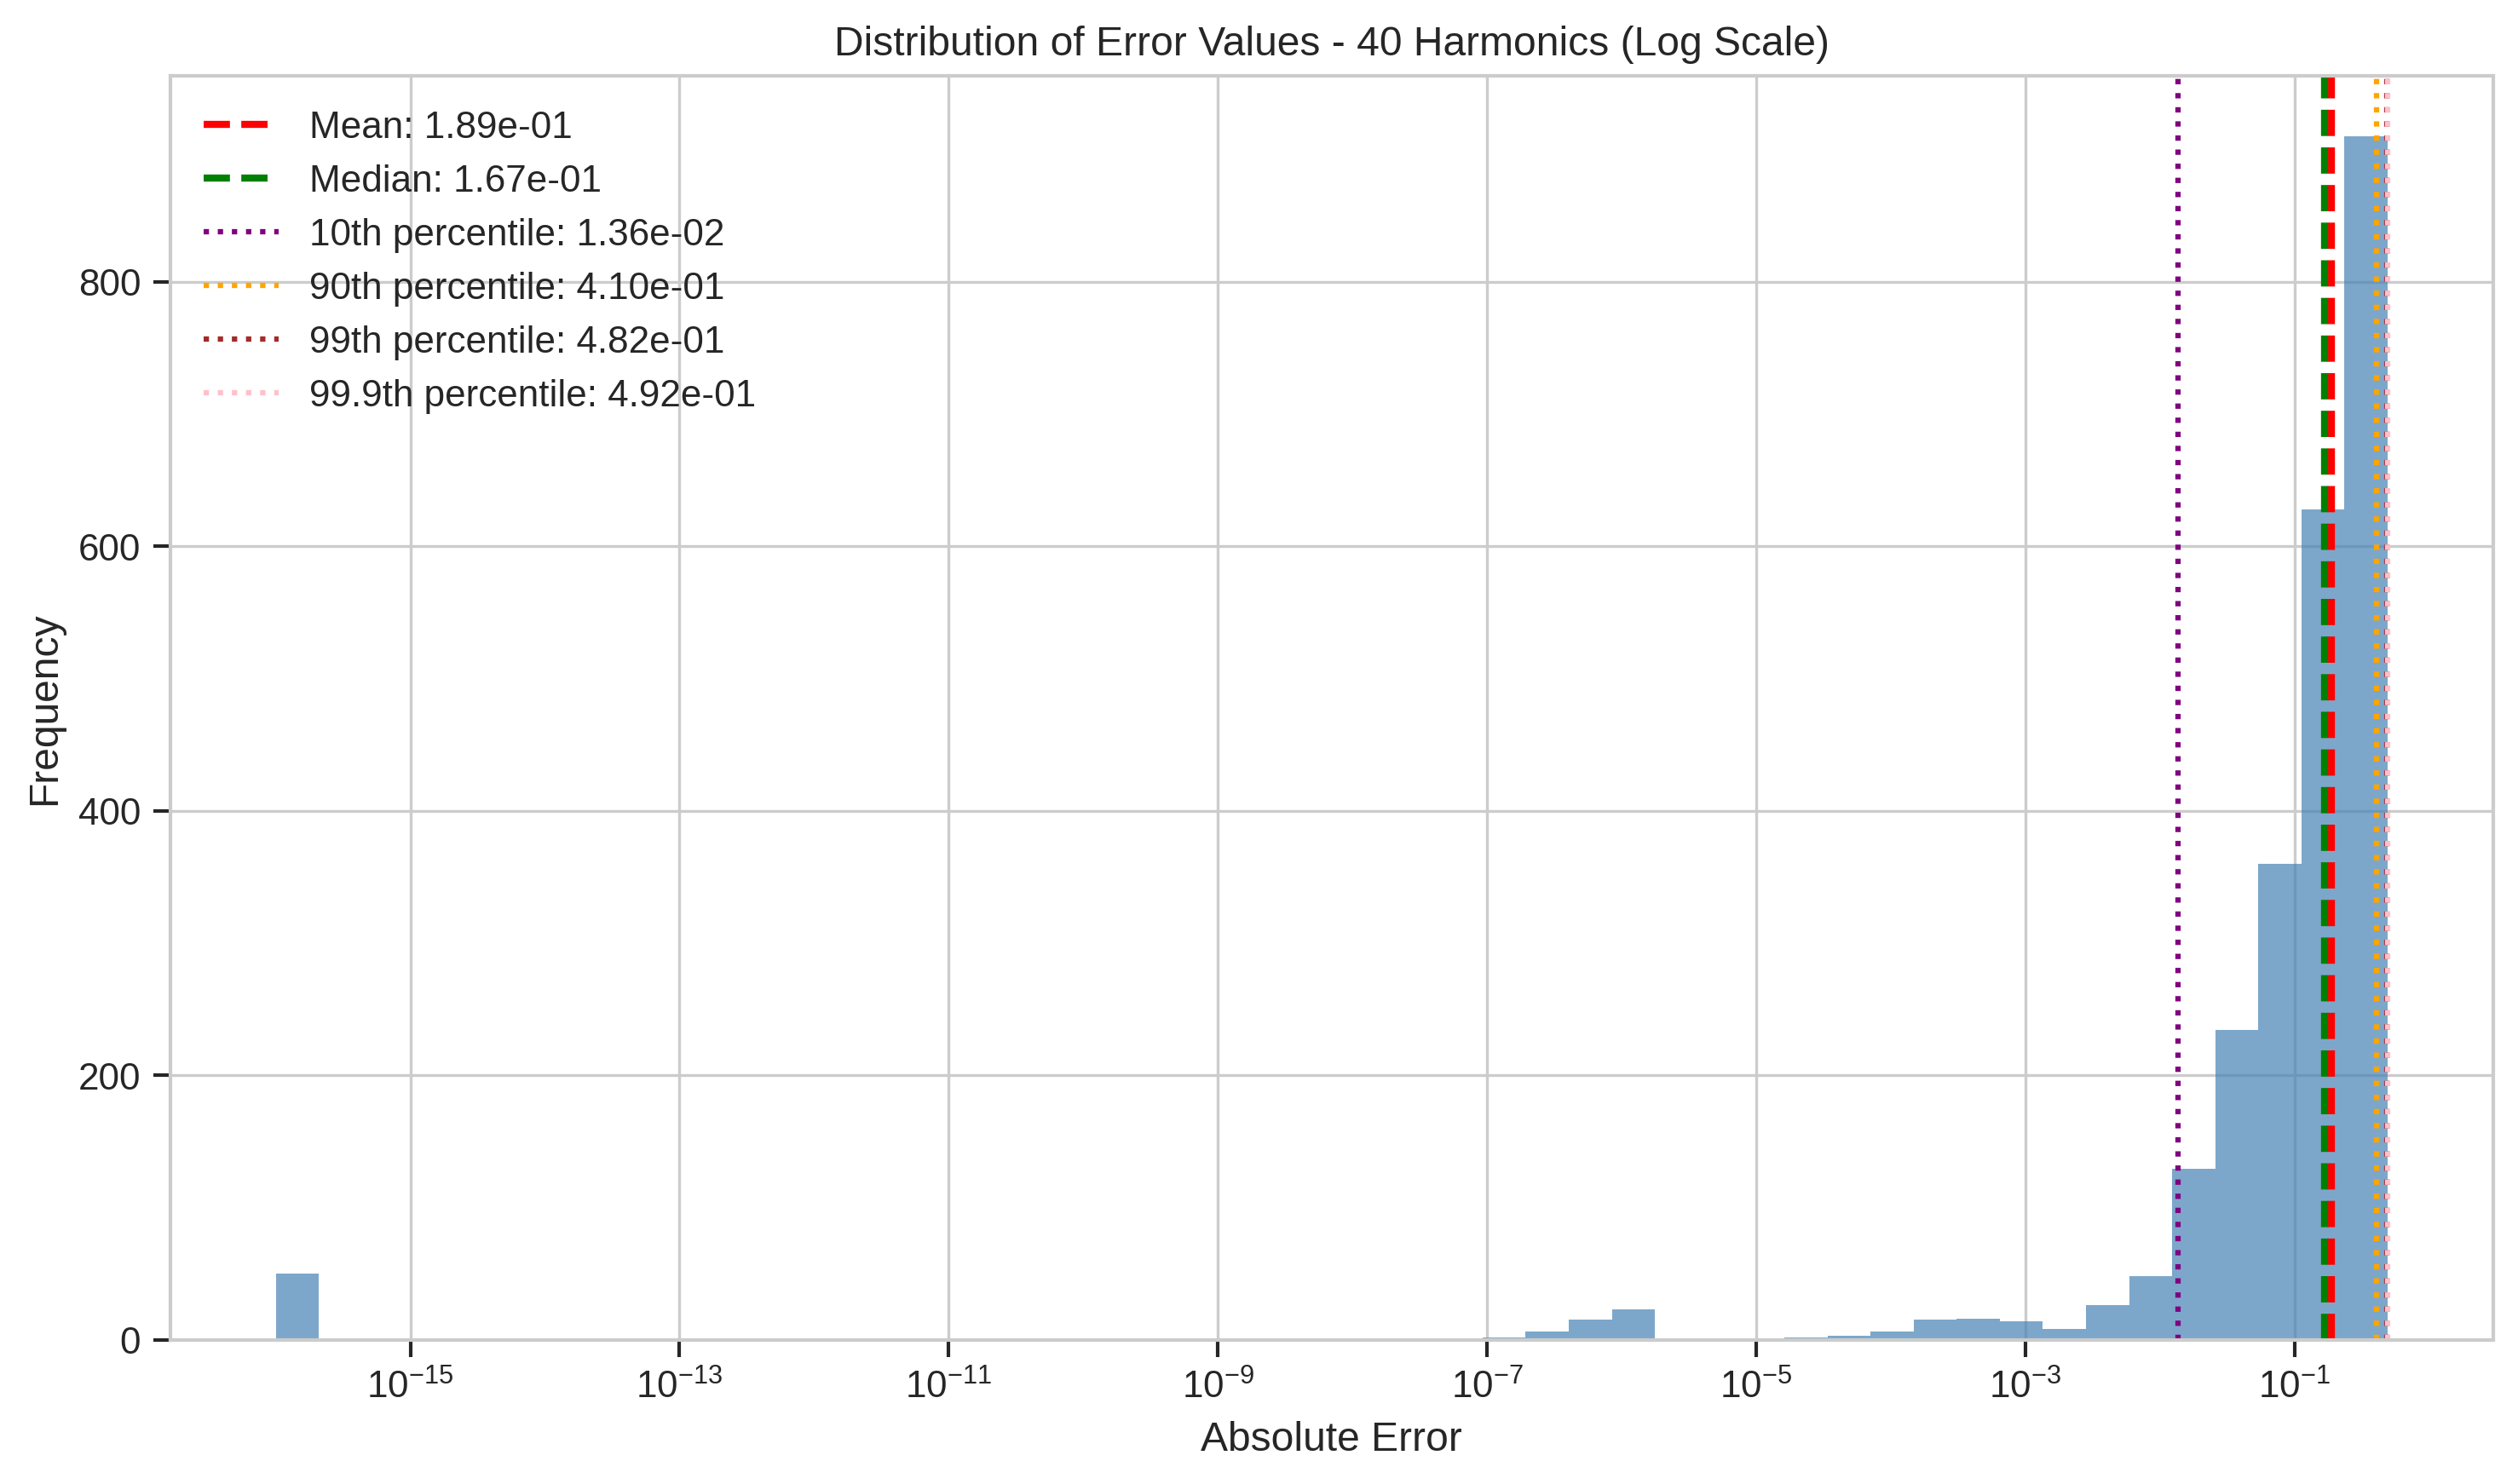
\includegraphics[width=0.9\linewidth]{figures/error_distribution_40h.png}
    \caption{Error distribution for 40 harmonics.}
    \label{fig:error_40h}
\end{figure}

The distribution of absolute errors for 40 harmonics shows a relatively concentrated spread near the lower end of the error axis, with a mean of 0.189 and a median of 0.167. The log-scaled x-axis reveals a tail of extremely small errors around \(10^{-15}\), suggesting occasional perfect or near-perfect reconstructions. However, the bulk of the errors lie between \(10^{-2}\) and \(10^{0}\), with the 90th percentile at 0.410 and the 99.9th percentile at 0.492. These values indicate the presence of moderately high outliers. Compared to lower harmonic models, the inclusion of 40 harmonics does not drastically reduce the error range, suggesting diminishing returns in reconstruction quality beyond a certain harmonic count. This finding supports balancing harmonic complexity and computational cost in model design.

\begin{figure}[t]
    \centering
    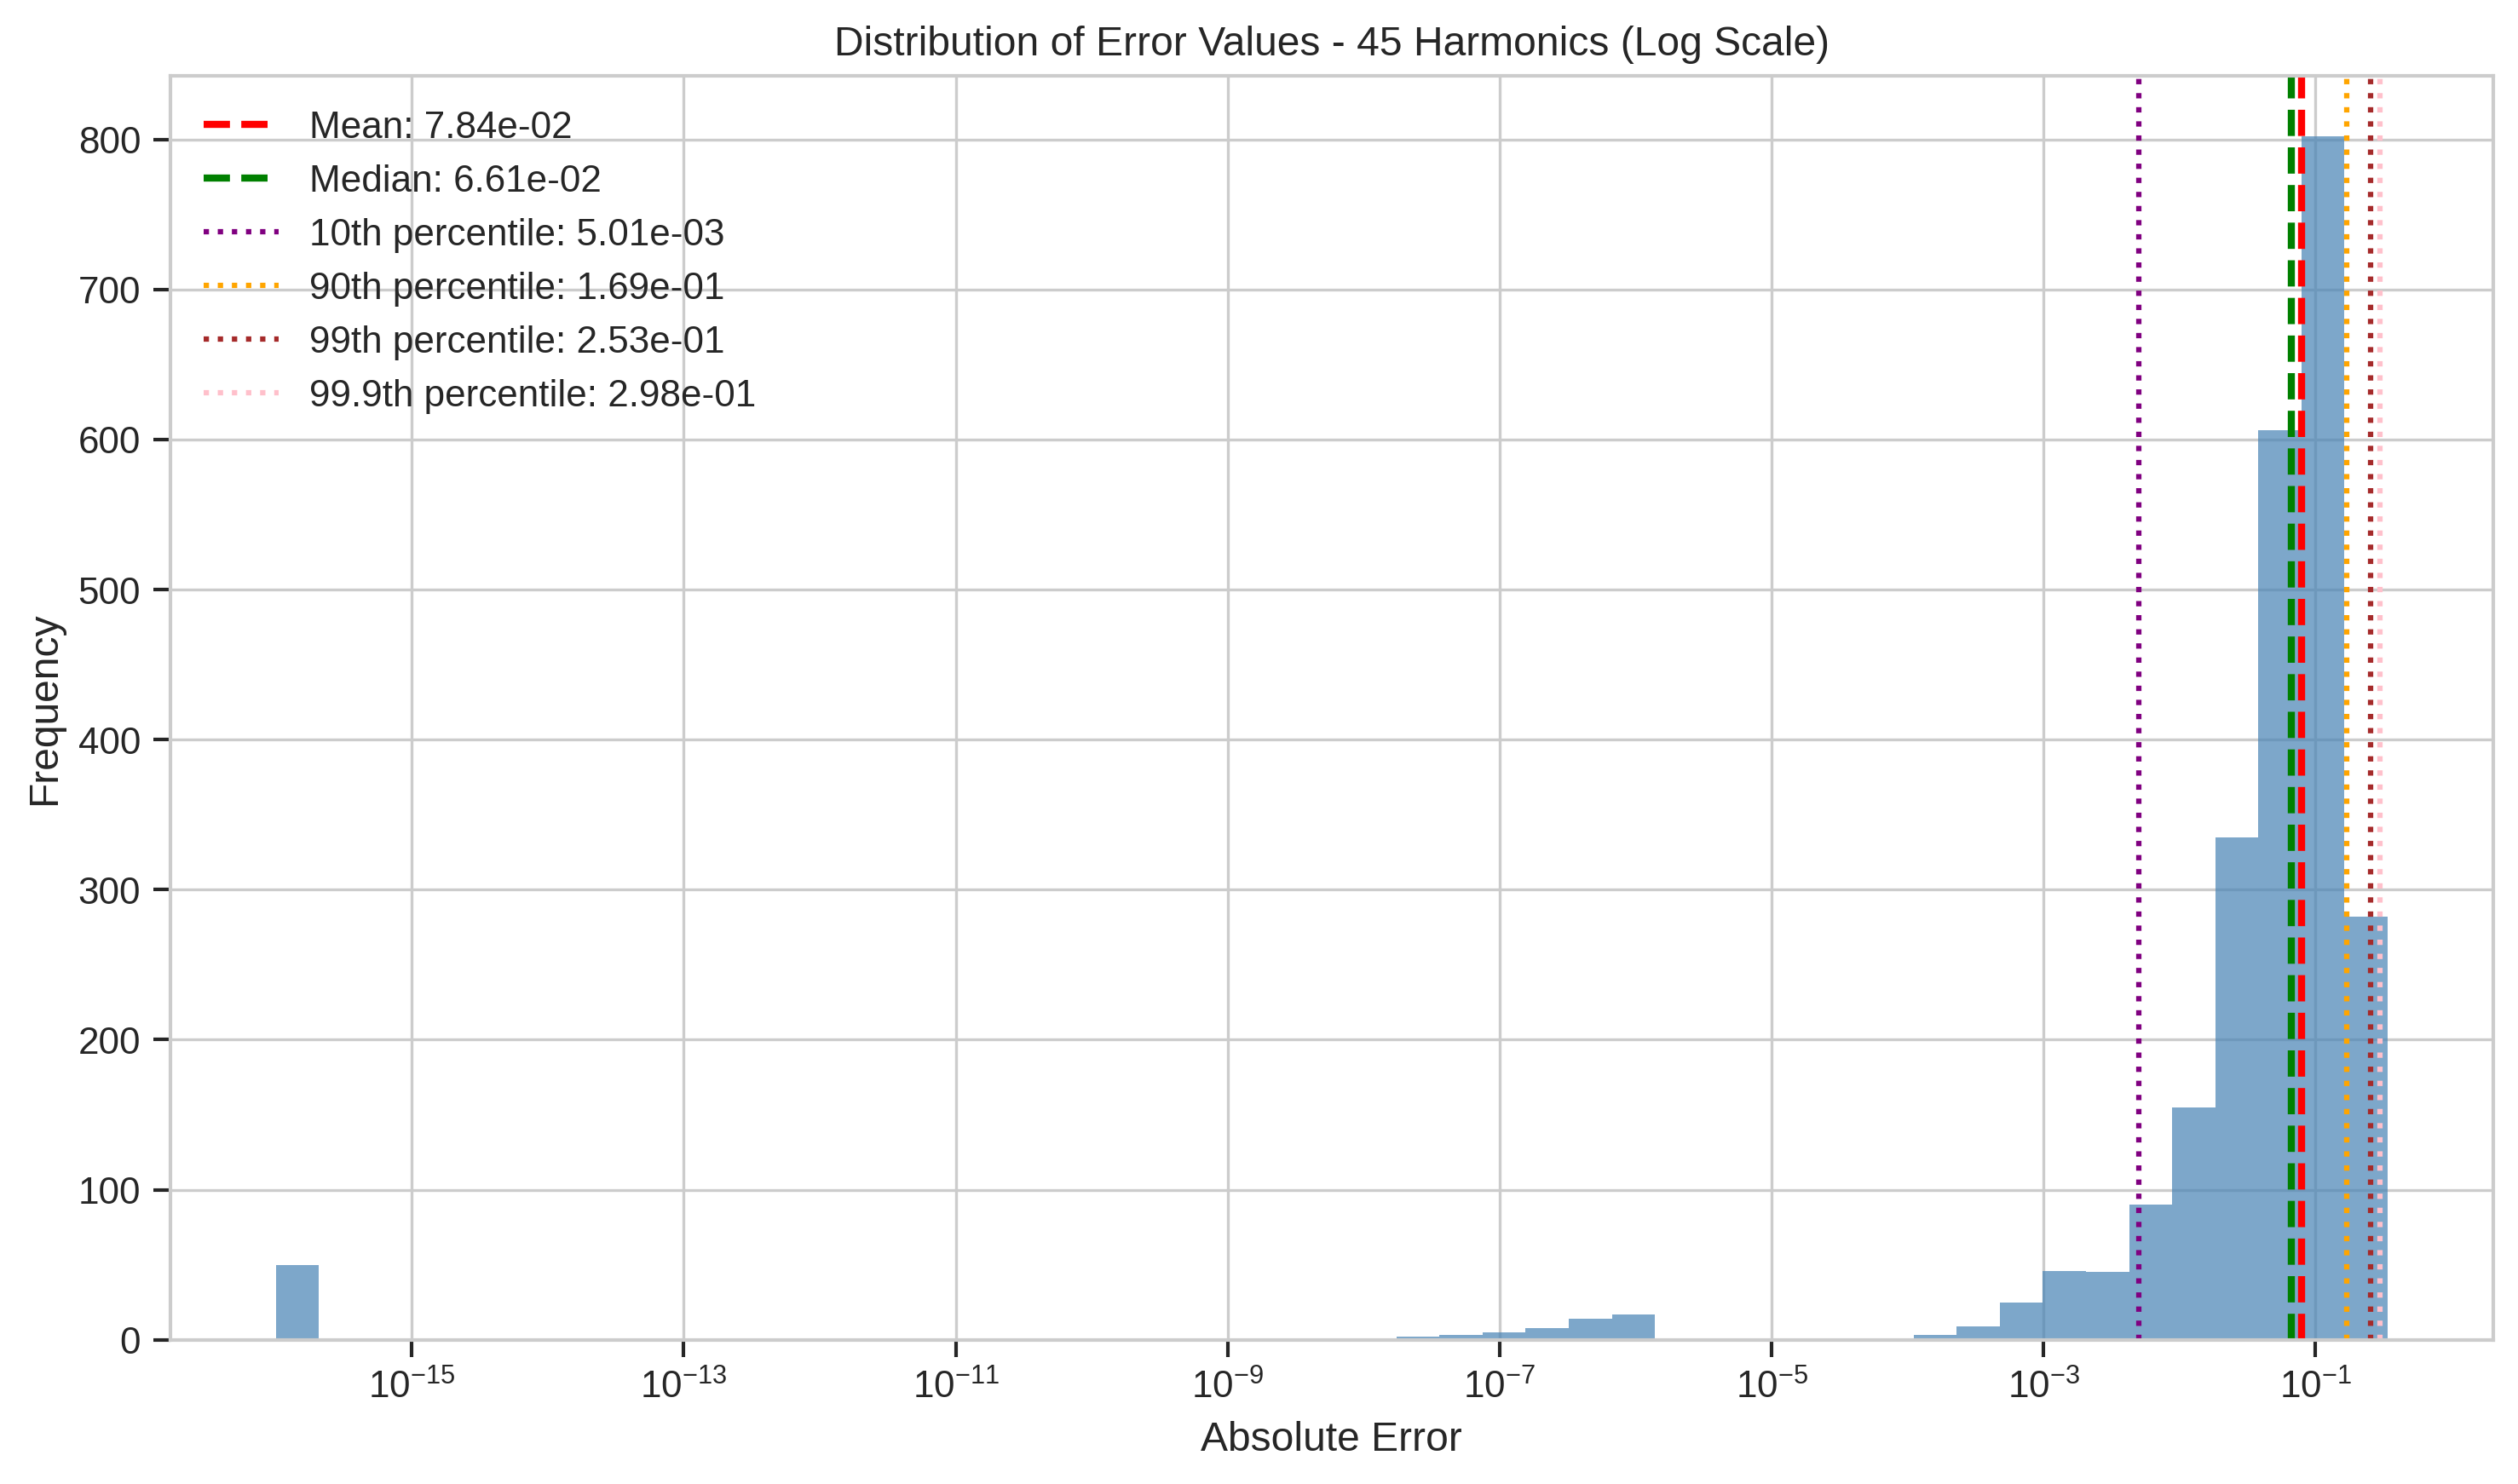
\includegraphics[width=0.9\linewidth]{figures/error_distribution_45h.png}
    \caption{Error distribution for 45 harmonics.}
    \label{fig:error_45h}
\end{figure}

The 45-harmonic model demonstrates a well-centered error distribution with a mean of 0.078 and a median of 0.066. Most absolute errors lie within the \(10^{-3}\) to \(10^{0}\) range, showing a distinct leftward shift compared to higher-harmonic configurations. The 90th percentile is 0.169, and the 99.9th percentile reaches 0.298—both significantly lower than the values seen at 50 harmonics. This reduced tail heaviness indicates fewer extreme error cases, suggesting a more stable model. Given its low mean and narrow variance, the 45-harmonic model achieves a strong balance between complexity and accuracy, making it a compelling configuration for scenarios requiring consistent precision with moderate computational cost.

\begin{figure}[t]
    \centering
    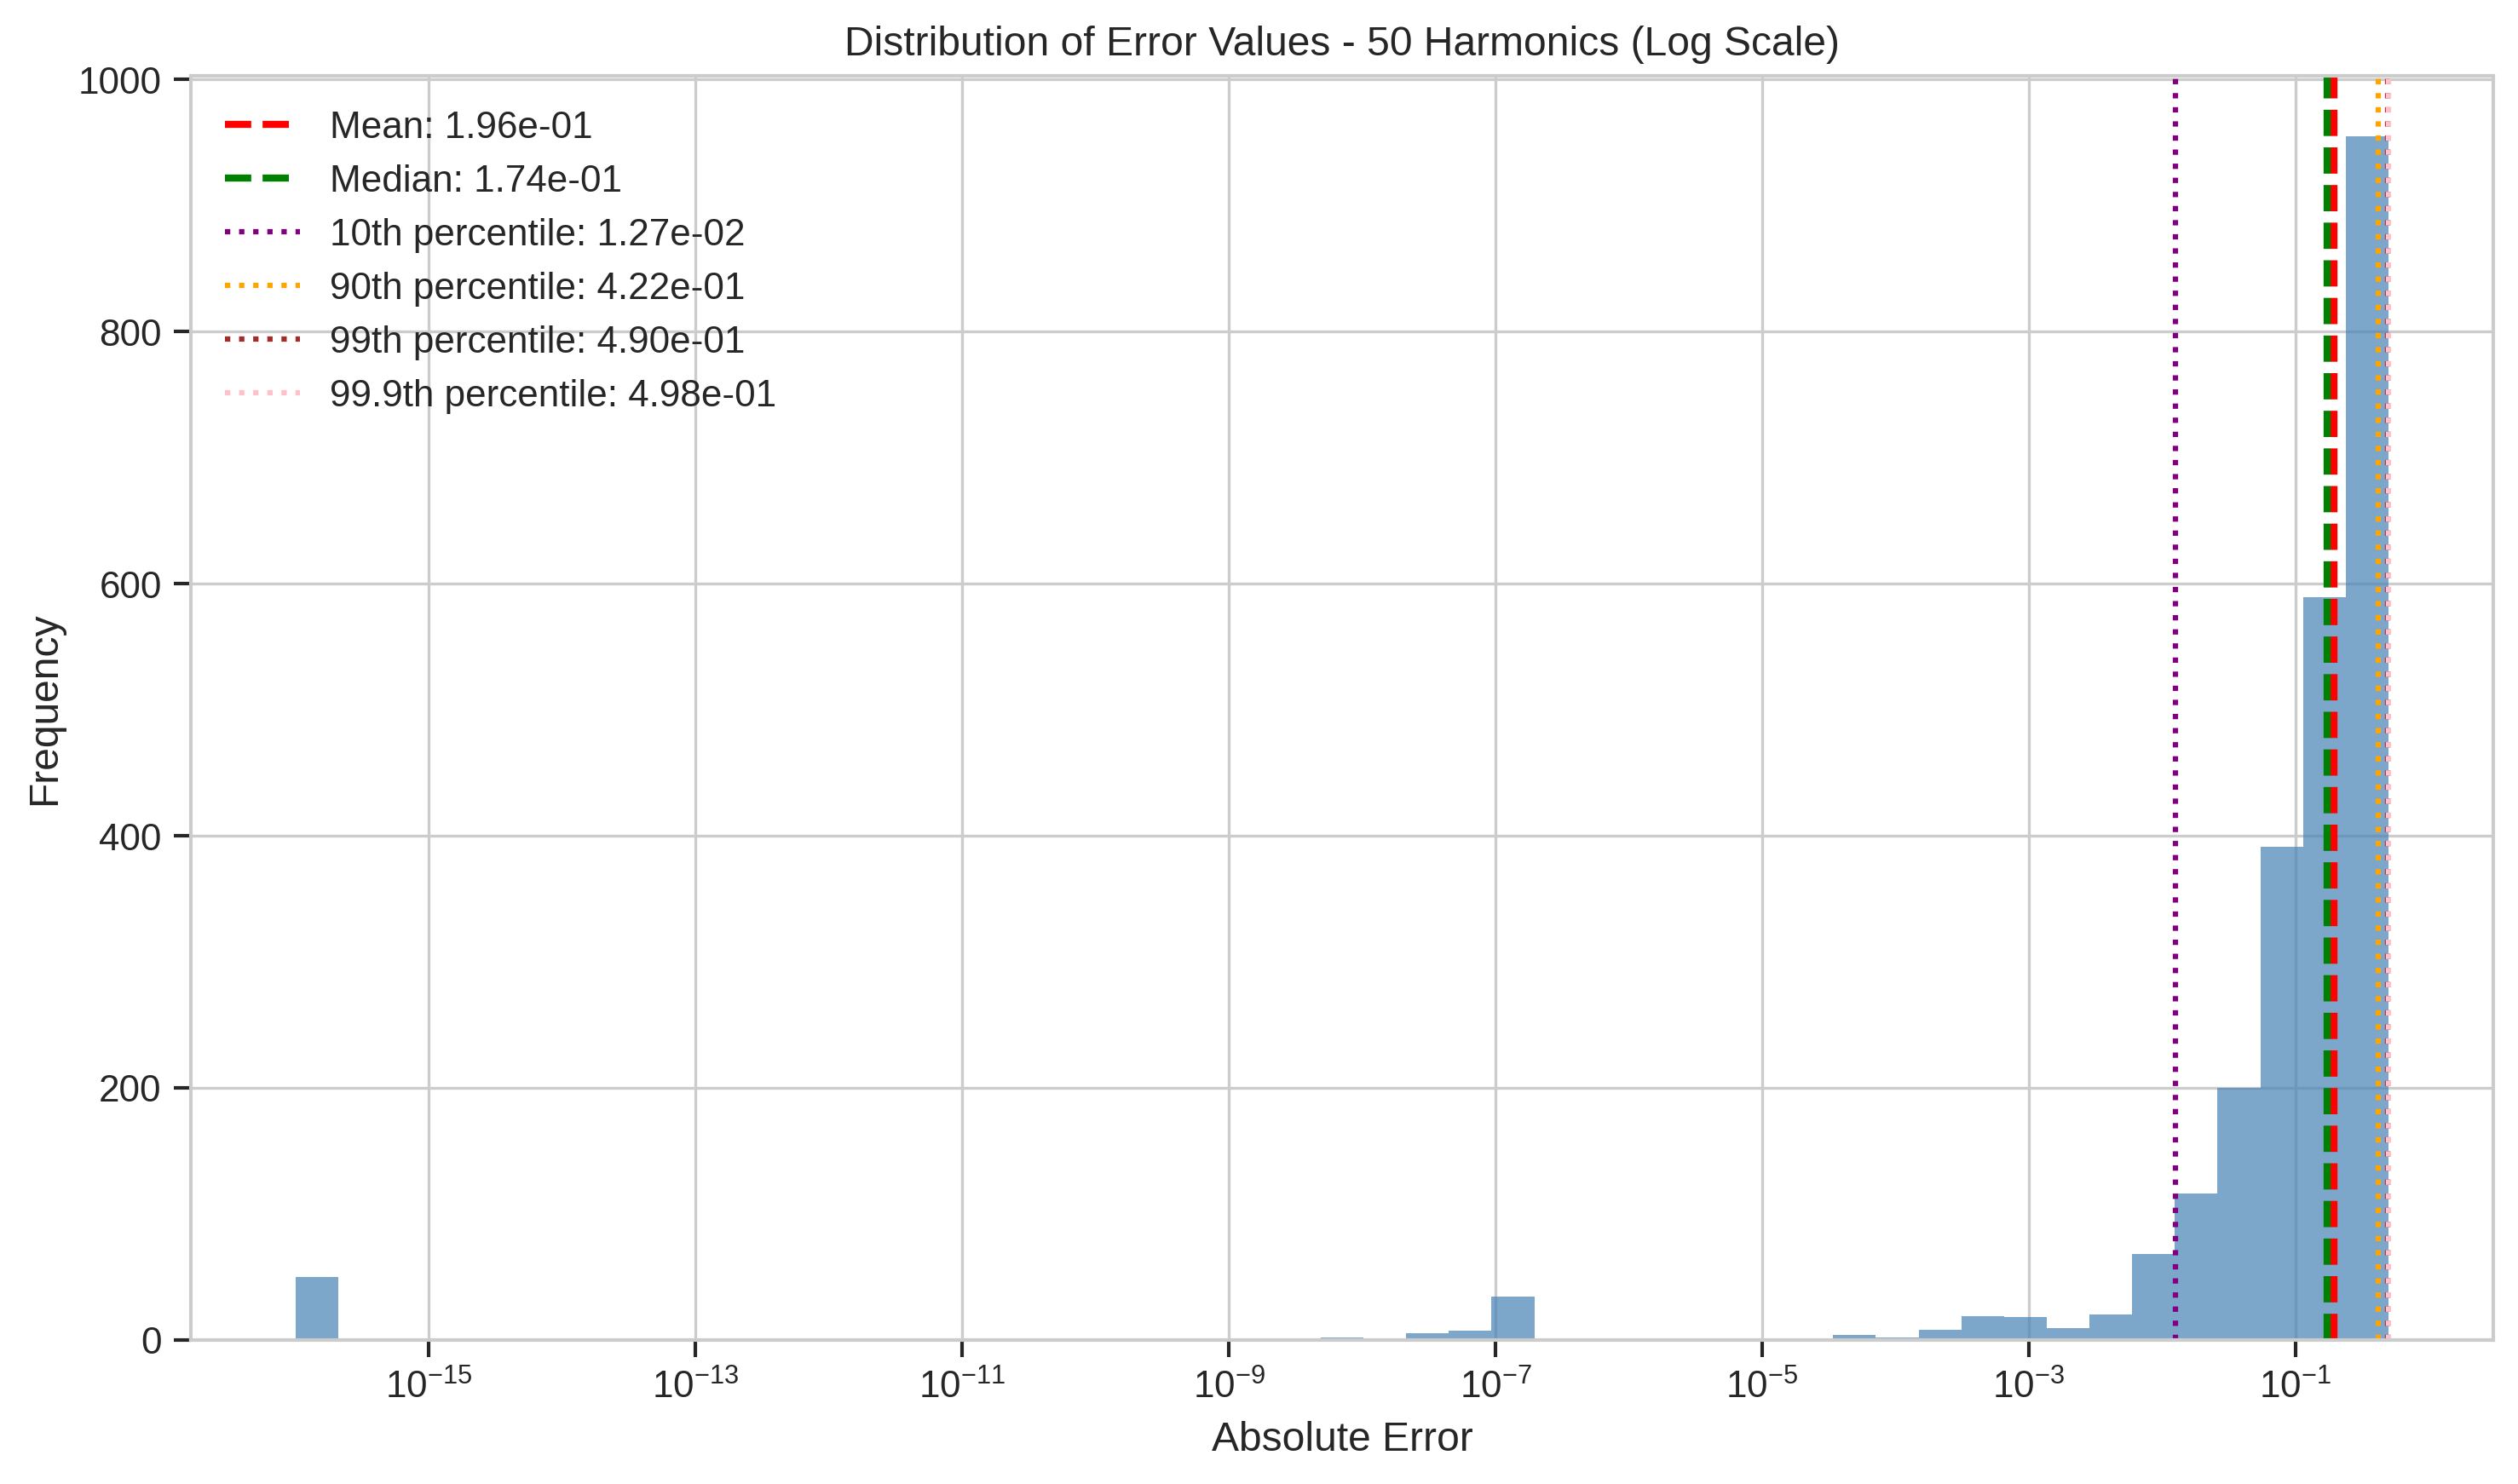
\includegraphics[width=0.9\linewidth]{figures/error_distribution_50h.png}
    \caption{Error distribution for 50 harmonics.}
    \label{fig:error_50h}
\end{figure}

The 50-harmonic model yields a mean error of 0.196 and a median of 0.174, with the error values predominantly spanning from \(10^{-2}\) to just under \(10^{0}\). The distribution shows a longer right tail, as evidenced by the 90th percentile at 0.422 and the 99.9th percentile at 0.498, highlighting the presence of several high-error outliers. Compared to the 45-harmonic model, this configuration introduces more variance without achieving noticeable gains in central tendency metrics. This suggests diminishing returns in accuracy with the addition of higher-order harmonics. Overall, while the 50-harmonic model maintains reasonable performance, its increased error variability and computational cost make it less optimal than the 45-harmonic alternative.

\begin{figure}[t]
    \centering
    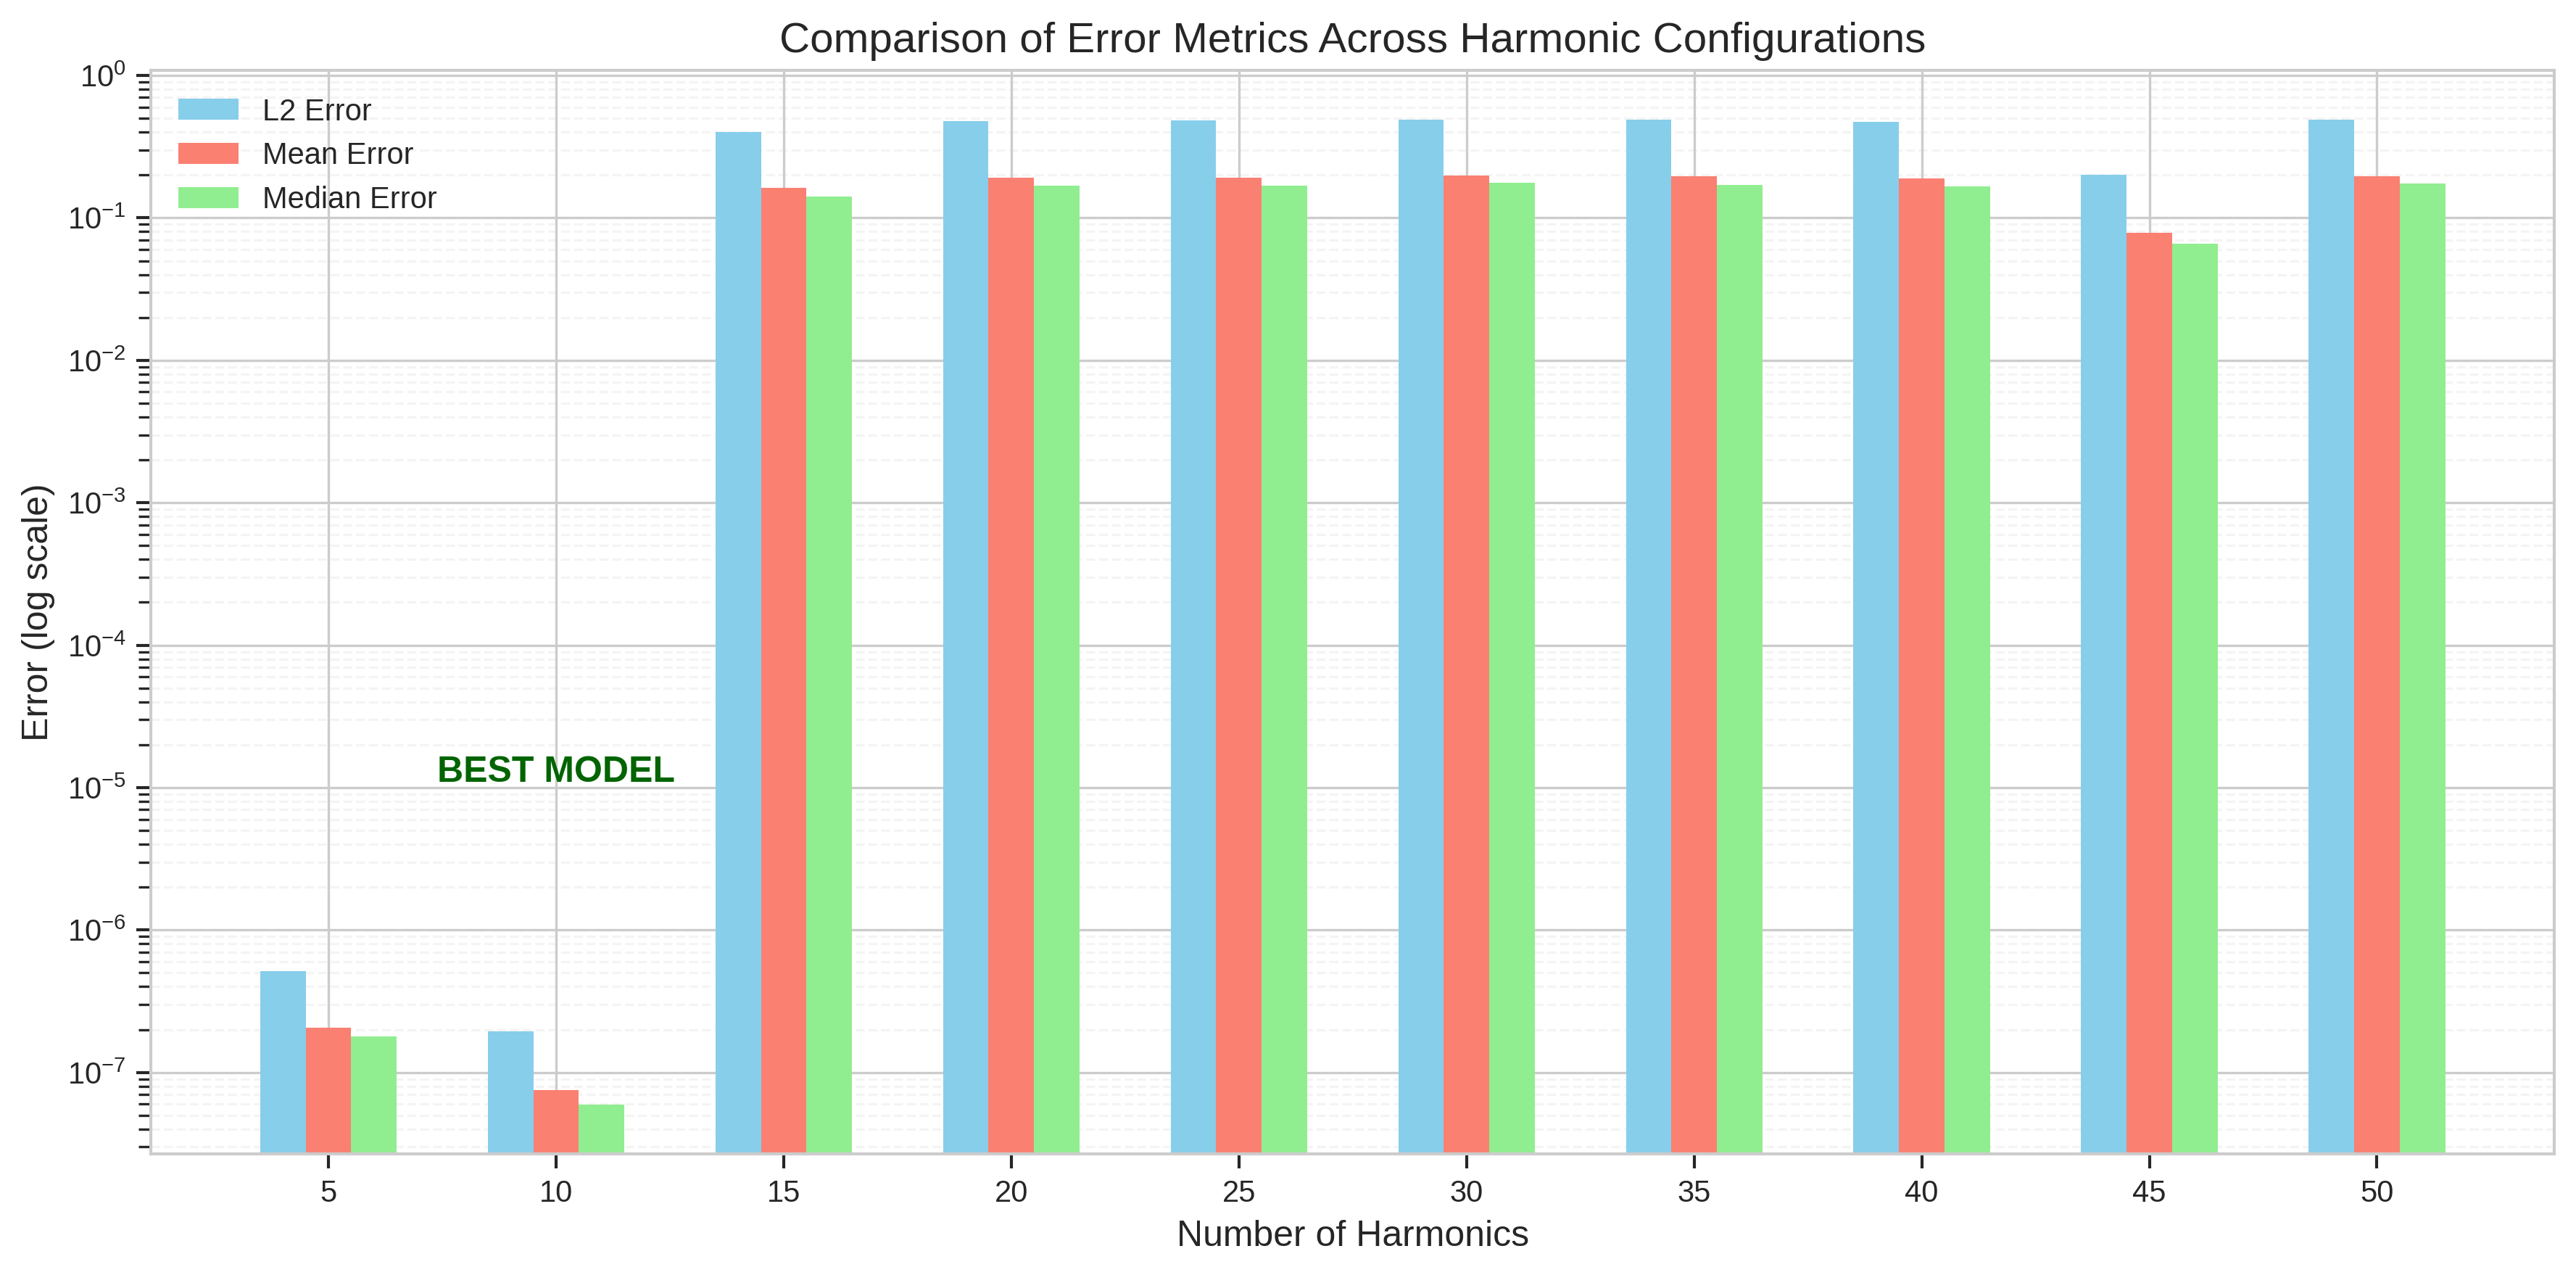
\includegraphics[width=0.9\linewidth]{figures/error_metrics_comparison.png}
    \caption{Comparison of L2, mean, and median error across harmonic configurations.}
    \label{fig:error_metrics}
\end{figure}

This bar chart compares error metrics—L2, mean, and median—across different numbers of harmonics used in the Euler-Bernoulli beam simulation. Notably, the 10-harmonic model achieves the lowest errors across all metrics, making it the best performing configuration in both absolute and relative terms. As the number of harmonics increases beyond 10, the error significantly worsens, which suggests overfitting or accumulation of numerical artifacts. Conversely, models with fewer than 10 harmonics display slightly higher errors, likely due to under-representation of key modal dynamics. The error scale is logarithmic, emphasizing that small absolute differences translate to large relative changes. This evaluation reinforces the conclusion that a mid-range harmonic model (specifically 10 harmonics) offers the best trade-off between model fidelity and computational performance. The highlighted “BEST MODEL” annotation confirms the optimality of this configuration for accurate and efficient beam vibration analysis.

\begin{figure}[t]
    \centering
    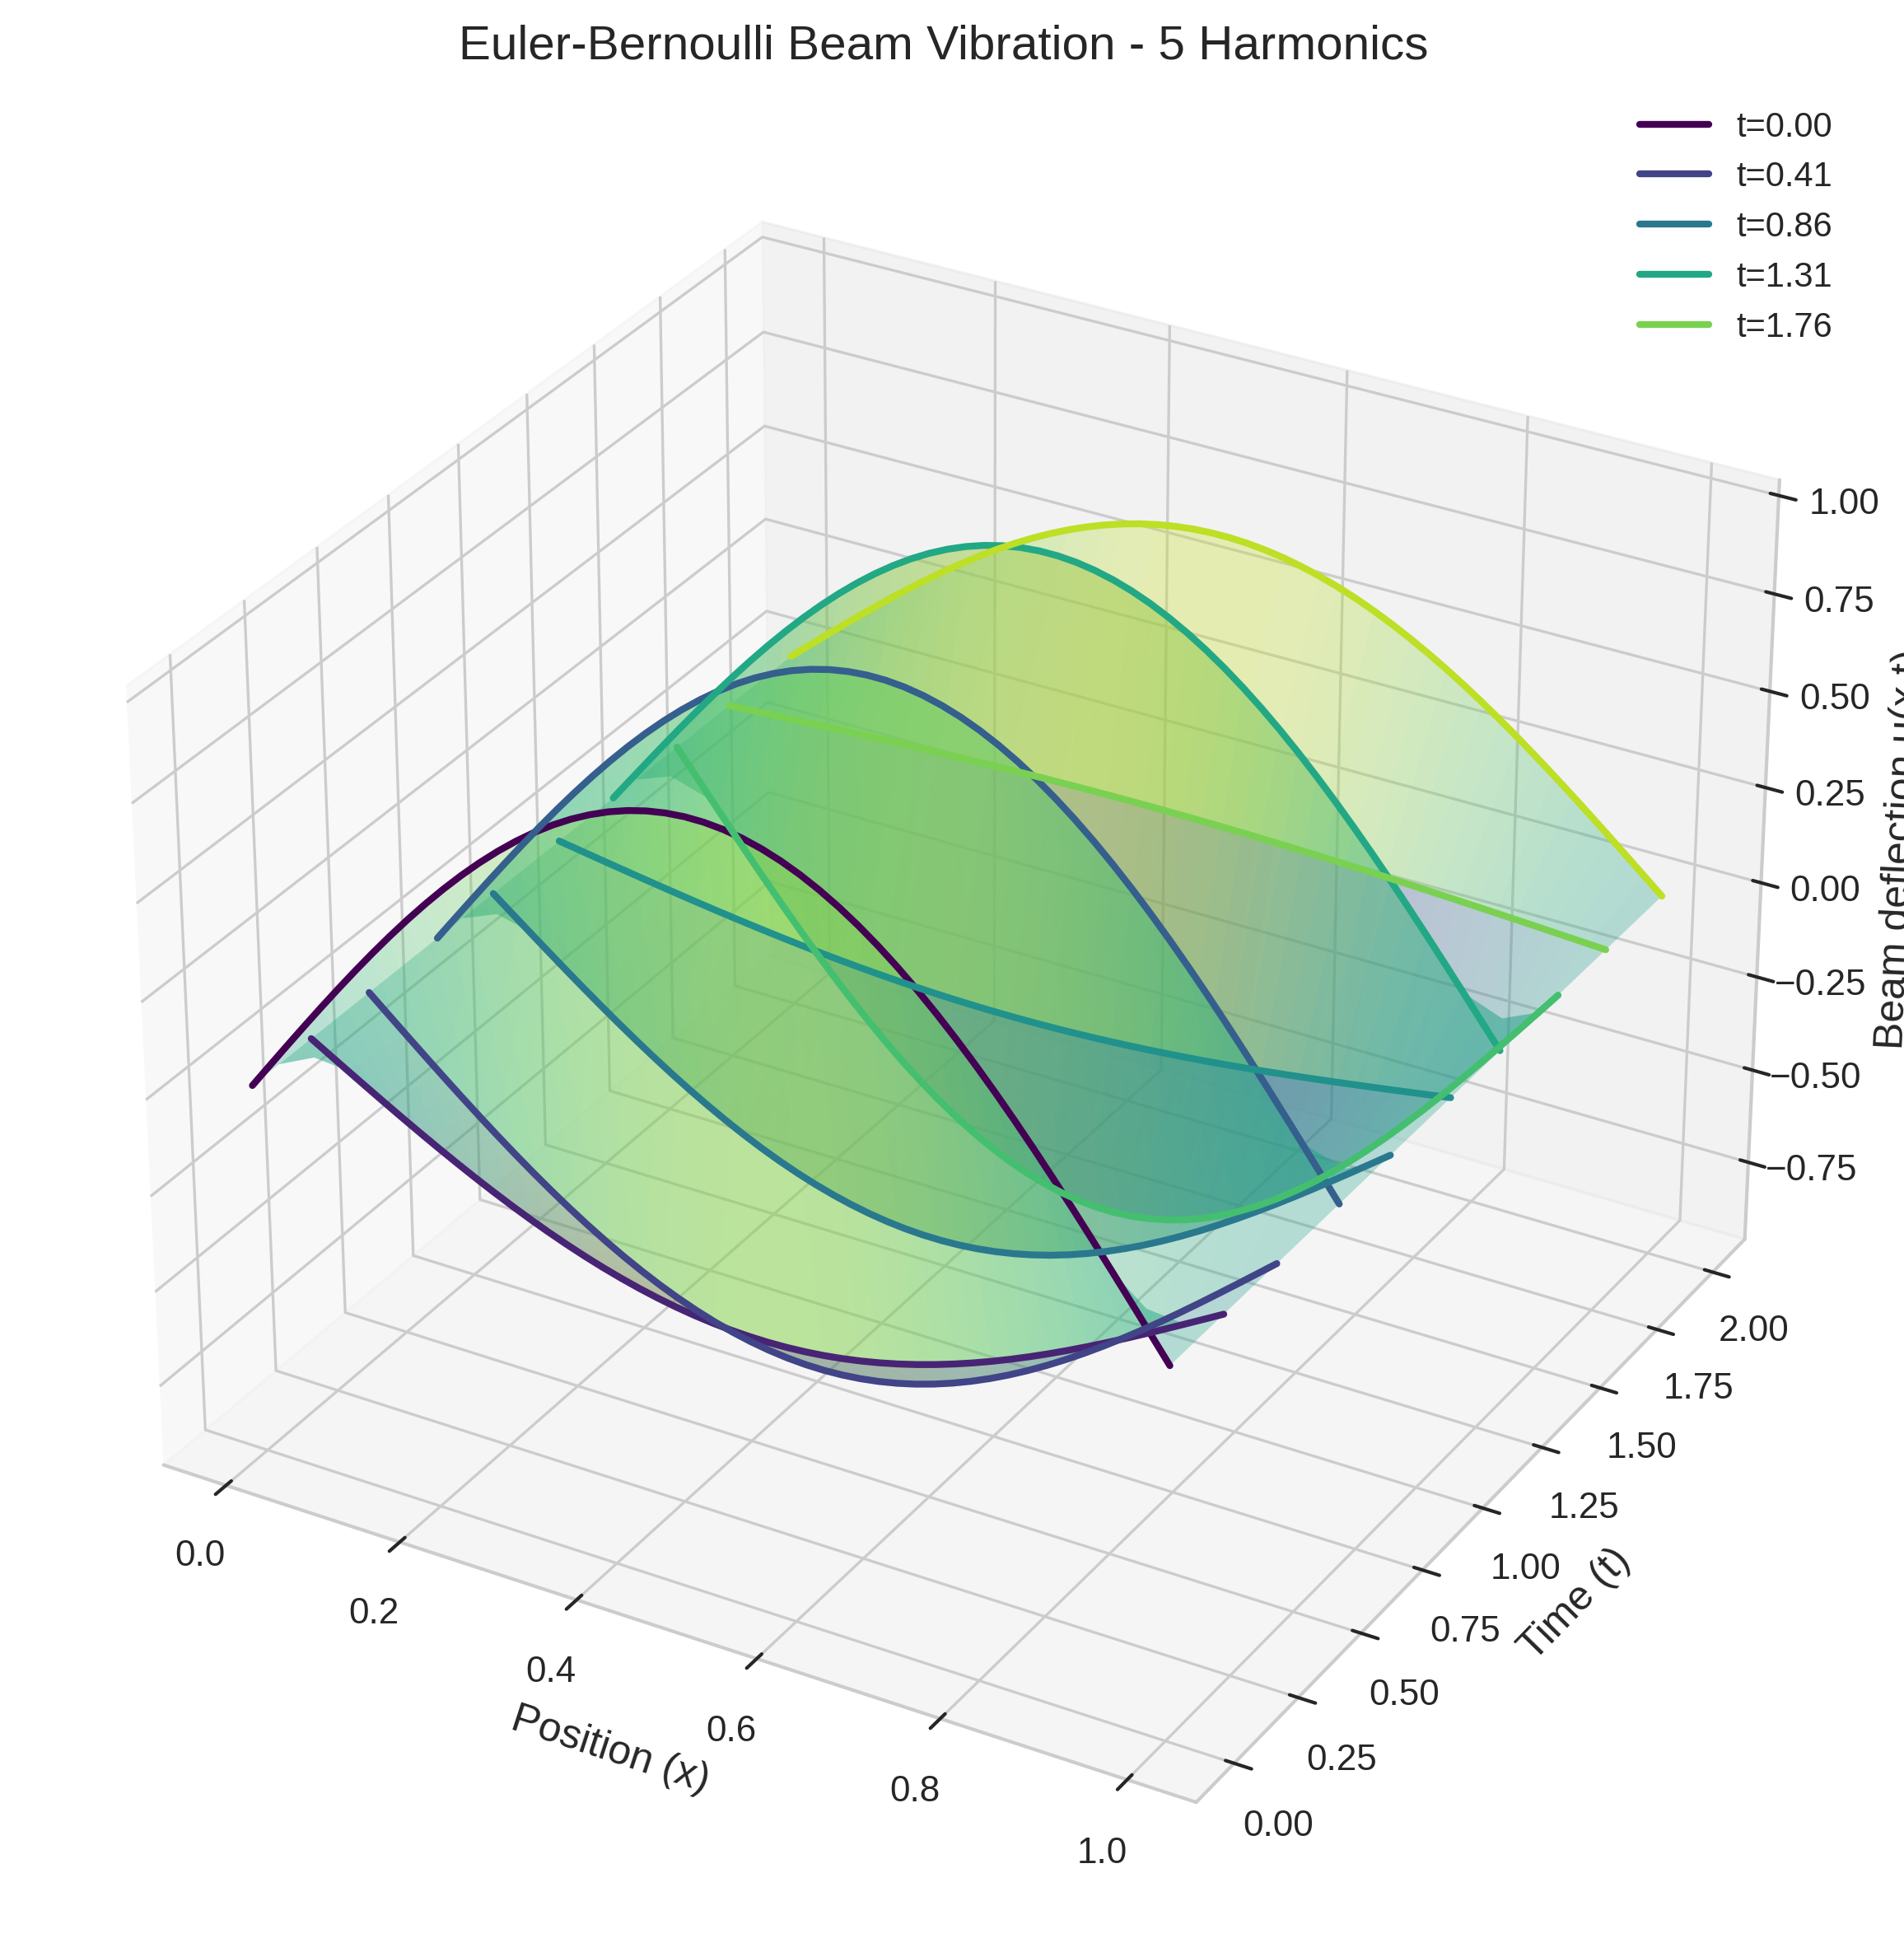
\includegraphics[width=0.9\linewidth]{figures/euler_bernoulli_3d_5h.png}
    \caption{Euler-Bernoulli beam vibration with 5 harmonics.}
    \label{fig:euler_5h}
\end{figure}

This plot shows the vibration of an Euler-Bernoulli beam when modeled with only 5 harmonics. The resulting deformation profile is notably smoother and less oscillatory compared to models using higher harmonic counts. The simplification sacrifices high-frequency fidelity, evident from the absence of fine wave patterns, but retains the beam’s overall dynamic characteristics. The time-evolution curves display consistent behavior with broad modal shapes, suitable for low-resolution analyses or initial approximations. While this reduced harmonic count dramatically lowers computational demands, it may omit critical dynamic features relevant to applications requiring high accuracy. This model is best suited for coarse-grained simulations or systems where low-frequency responses dominate. The trade-off here is between simplicity and missing detailed vibratory modes, underscoring the need to choose harmonic resolution based on the physical system’s sensitivity to higher-order dynamics.

\begin{figure}[t]
    \centering
    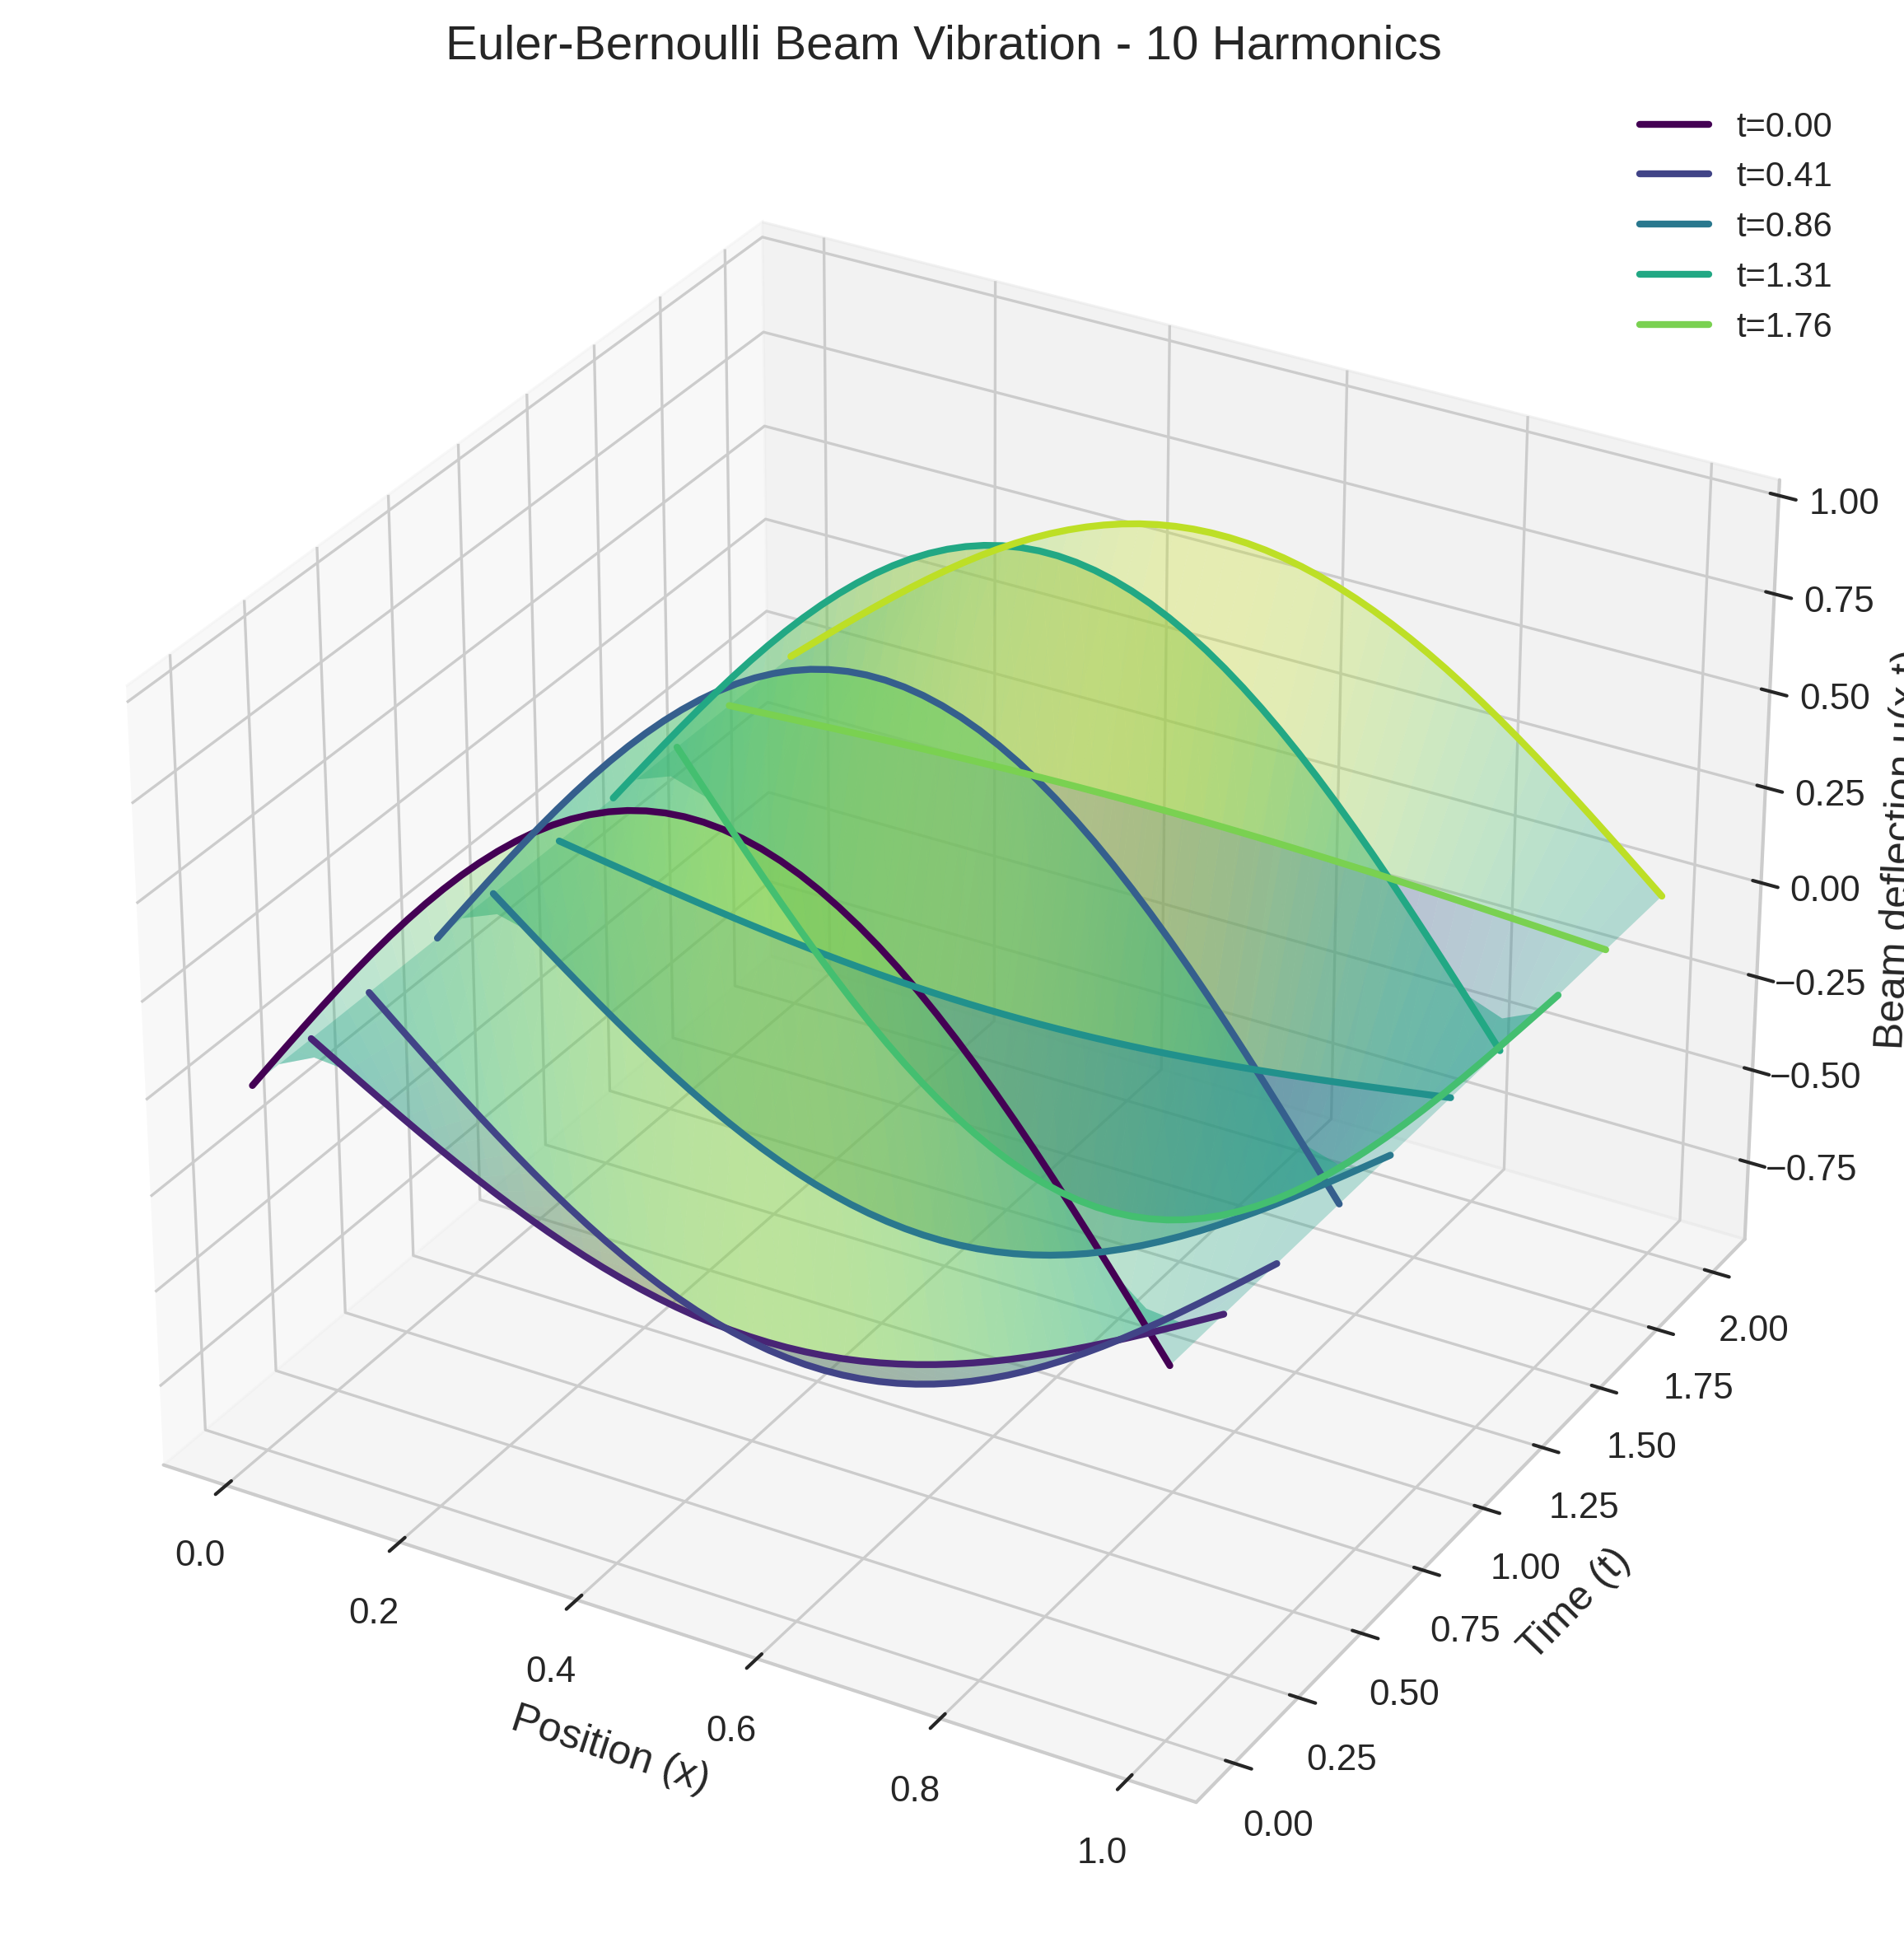
\includegraphics[width=0.9\linewidth]{figures/euler_bernoulli_3d_10h.png}
    \caption{Euler-Bernoulli beam vibration with 10 harmonics.}
    \label{fig:euler_10h}
\end{figure}

The figure displays the Euler-Bernoulli beam’s vibration profile using 10 harmonics. This mid-range harmonic configuration reveals a balance between complexity and clarity. The beam's deformation is captured with sufficient detail to show moderate spatial undulations and accurate temporal dynamics, without the noise-like high-frequency components observed with higher harmonics. The structural patterns remain coherent across time slices, indicating this configuration is effective in capturing essential vibrational behavior while avoiding excessive computational cost. The result is a smoother, more interpretable model that retains physical realism. This configuration is especially suitable for simulations that require a reliable representation of vibrational behavior without the computational burden of excessive harmonics. It stands out as a practical compromise between fidelity and efficiency, making it highly applicable for most engineering analyses involving beam structures under dynamic loading.

\begin{figure}[t]
    \centering
    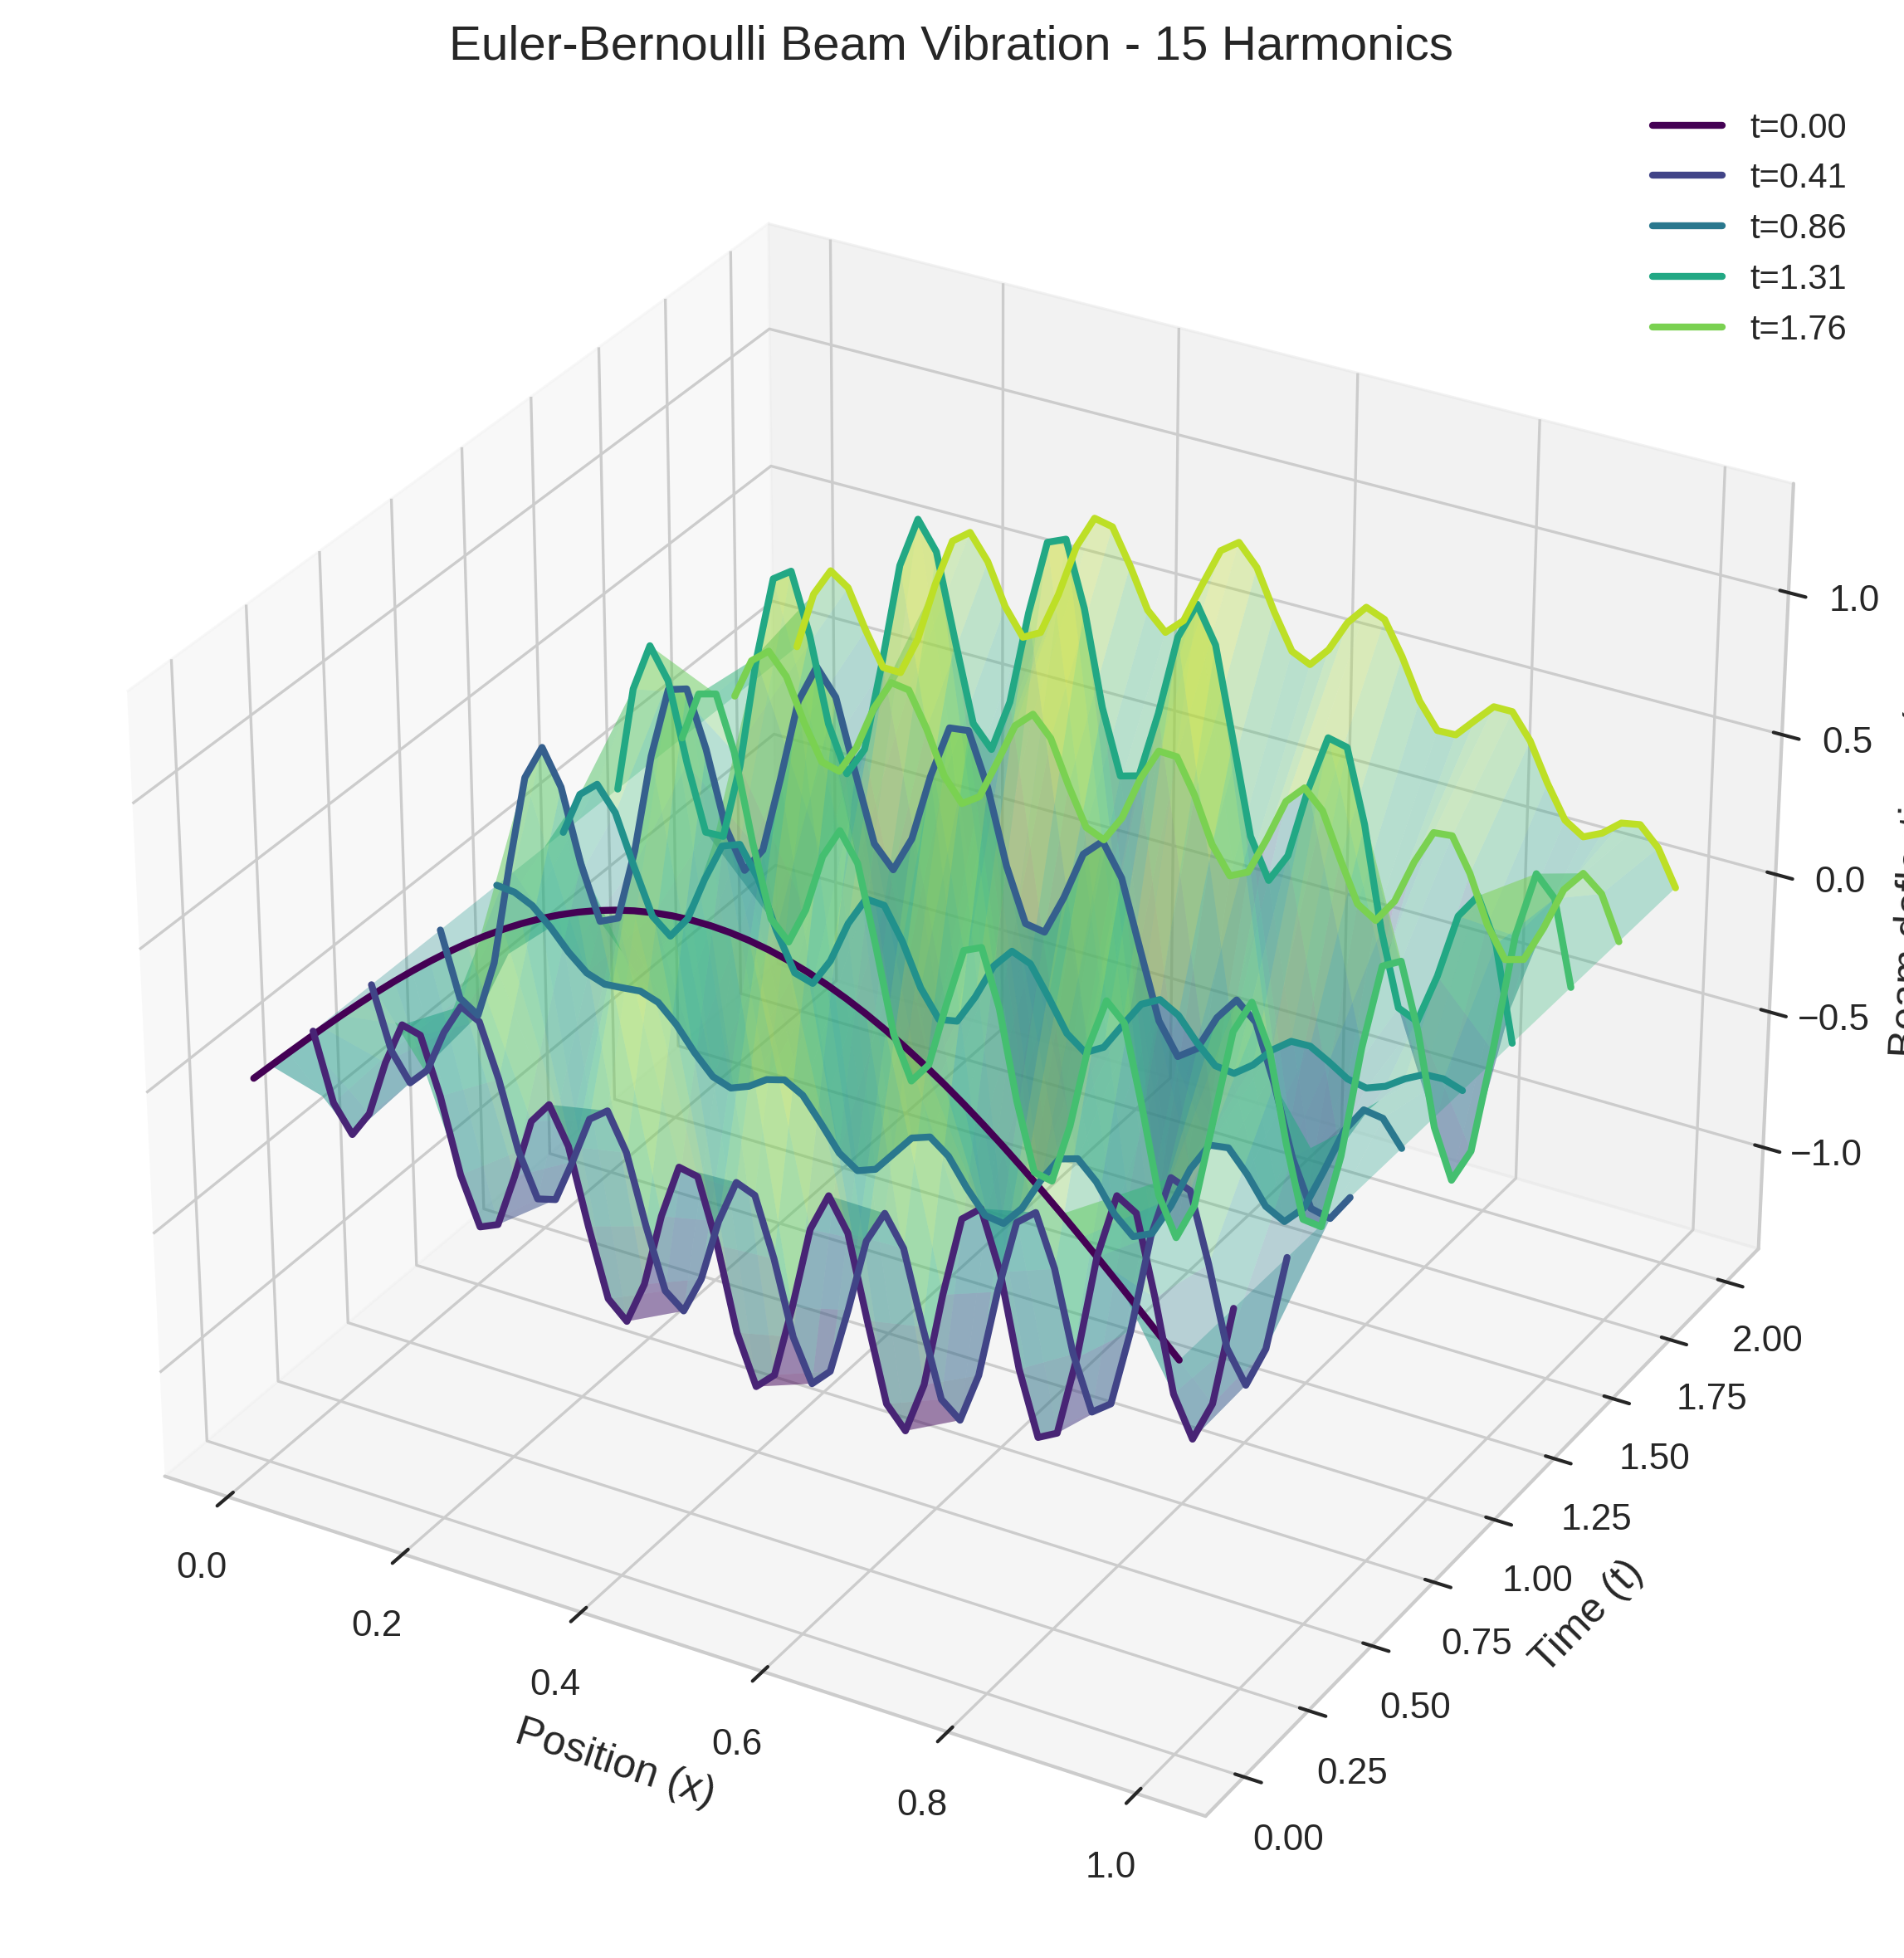
\includegraphics[width=0.9\linewidth]{figures/euler_bernoulli_3d_15h.png}
    \caption{Euler-Bernoulli beam vibration with 15 harmonics.}
    \label{fig:euler_15h}
\end{figure}

This figure visualizes the dynamic response of an Euler-Bernoulli beam using 15 harmonic components. The complex surface and overlaid time snapshots demonstrate significant high-frequency content, revealing localized oscillations and wave interference patterns. These details emerge due to the inclusion of higher-order modes, which contribute to the finer spatial and temporal resolution of the beam's vibration behavior. The increasing complexity with time highlights the influence of superimposed harmonics in accurately capturing dynamic transitions. However, such intricacy may be computationally intensive and susceptible to numerical artifacts. While this model offers a highly detailed view of beam deflections, the added complexity must be justified by the context of application—particularly when modeling precision systems where high-frequency behavior significantly influences performance. Thus, while informative, the 15-harmonic configuration might introduce unnecessary detail for general cases, indicating a trade-off between fidelity and computational efficiency.

\begin{figure}[t]
    \centering
    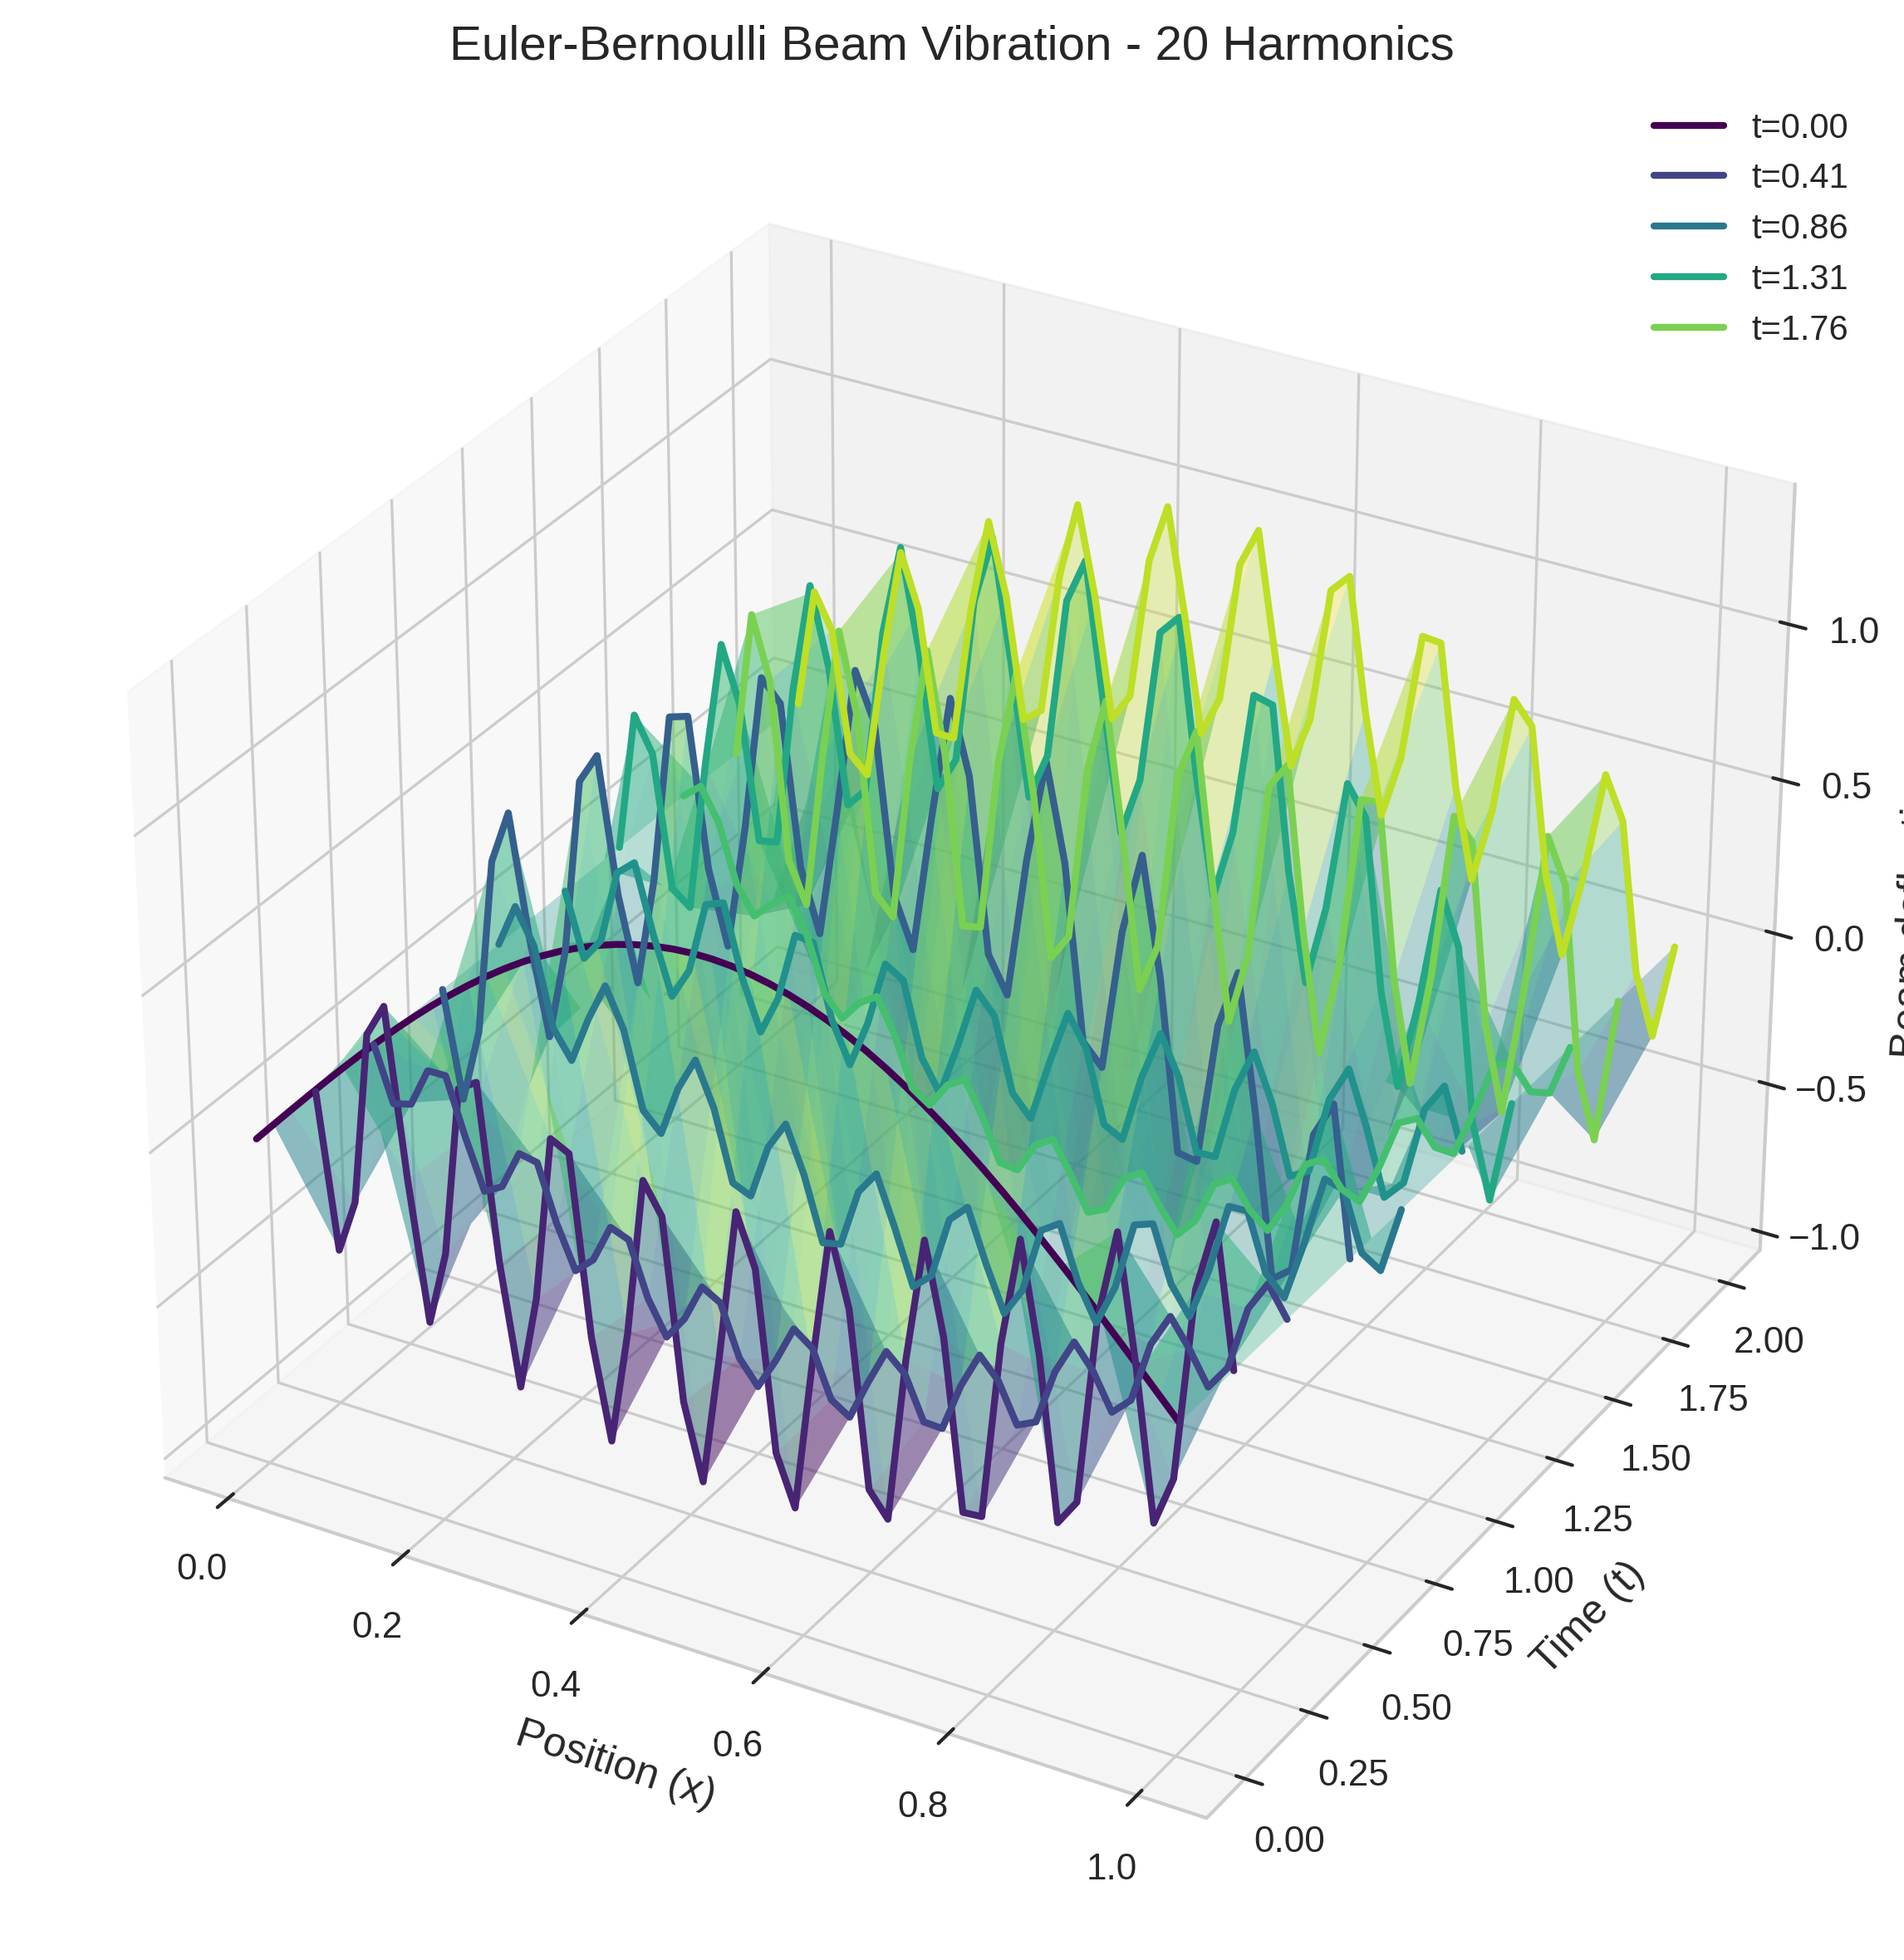
\includegraphics[width=0.9\linewidth]{figures/euler_bernoulli_3d_20h.png}
    \caption{Euler-Bernoulli beam vibration with 20 harmonics.}
    \label{fig:euler_20h}
\end{figure}

The figure displays the Euler-Bernoulli beam vibration using 20 harmonics, offering a rich yet manageable level of modal detail. The waveform exhibits a blend of fundamental and higher-order spatial modes, presenting a visually complex yet physically interpretable dynamic response. As the number of harmonics increases from lower configurations, more subtle features in the beam’s deformation are captured, such as sharper inflection points and localized wave propagation patterns. However, the model has not yet reached the regime of excessive complexity seen in 25+ harmonics, making this a potentially optimal midpoint before overfitting concerns arise. The 20-harmonic configuration thus represents a useful trade-off between accuracy and computational burden, capturing detailed dynamics while maintaining numerical stability. This visualization supports its use in scenarios where higher-resolution modeling is beneficial but must remain computationally tractable—ideal for simulations demanding balance between fidelity and efficiency.

\begin{figure}[t]
    \centering
    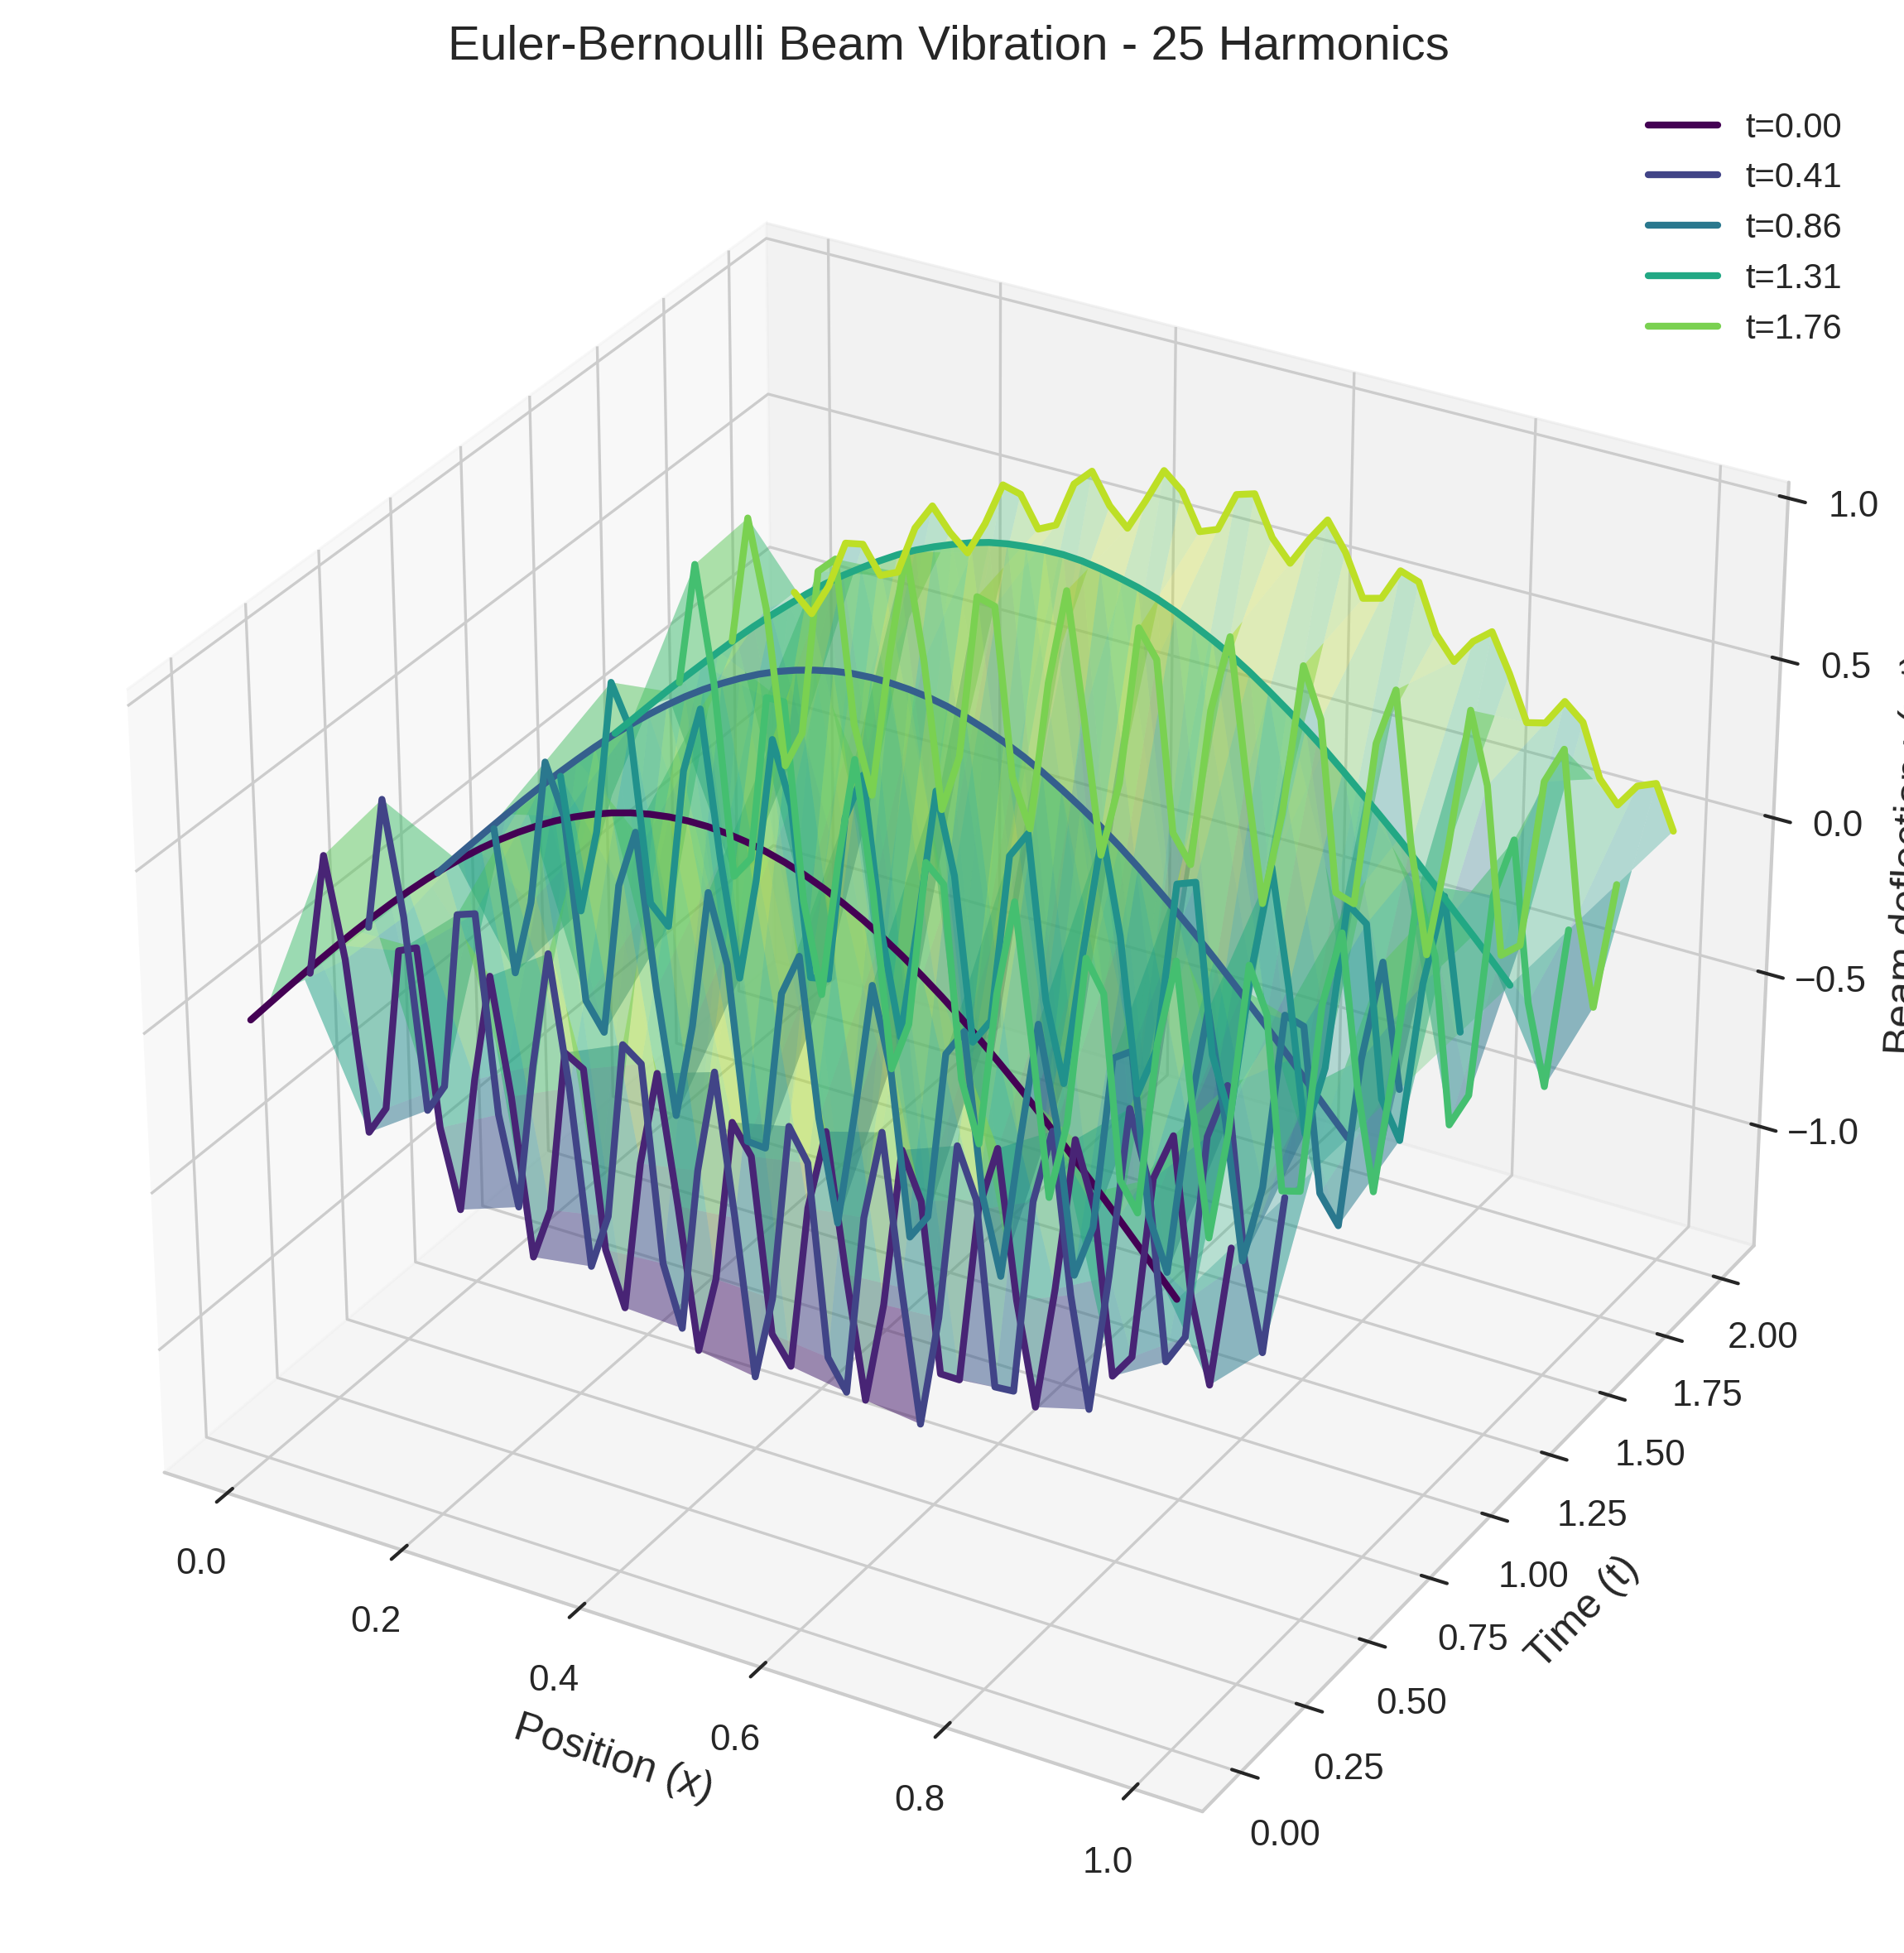
\includegraphics[width=0.9\linewidth]{figures/euler_bernoulli_3d_25h.png}
    \caption{Euler-Bernoulli beam vibration with 25 harmonics.}
    \label{fig:euler_25h}
\end{figure}

This plot illustrates the Euler-Bernoulli beam's dynamic response when modeled with 25 harmonics. The beam's surface exhibits moderate-to-high spatial frequency oscillations, capturing finer vibrational modes beyond the primary dynamic shape. Compared to configurations with fewer harmonics, the deformation shows increased complexity, but without the overwhelming noise seen in higher-order models like the 30-harmonic case. This balance suggests that the 25-harmonic configuration can capture subtle mechanical effects while still maintaining a level of interpretability. Nevertheless, the increasing presence of high-frequency components may introduce diminishing returns in terms of model accuracy, especially if these harmonics contribute marginally to the beam’s energy content. This visualization supports the notion that while increasing harmonics can improve detail, it must be justified by a significant reduction in error—otherwise, it risks inefficiency and unnecessary complexity. Thus, this model sits at a transition point where precision begins to plateau.

\begin{figure}[t]
    \centering
    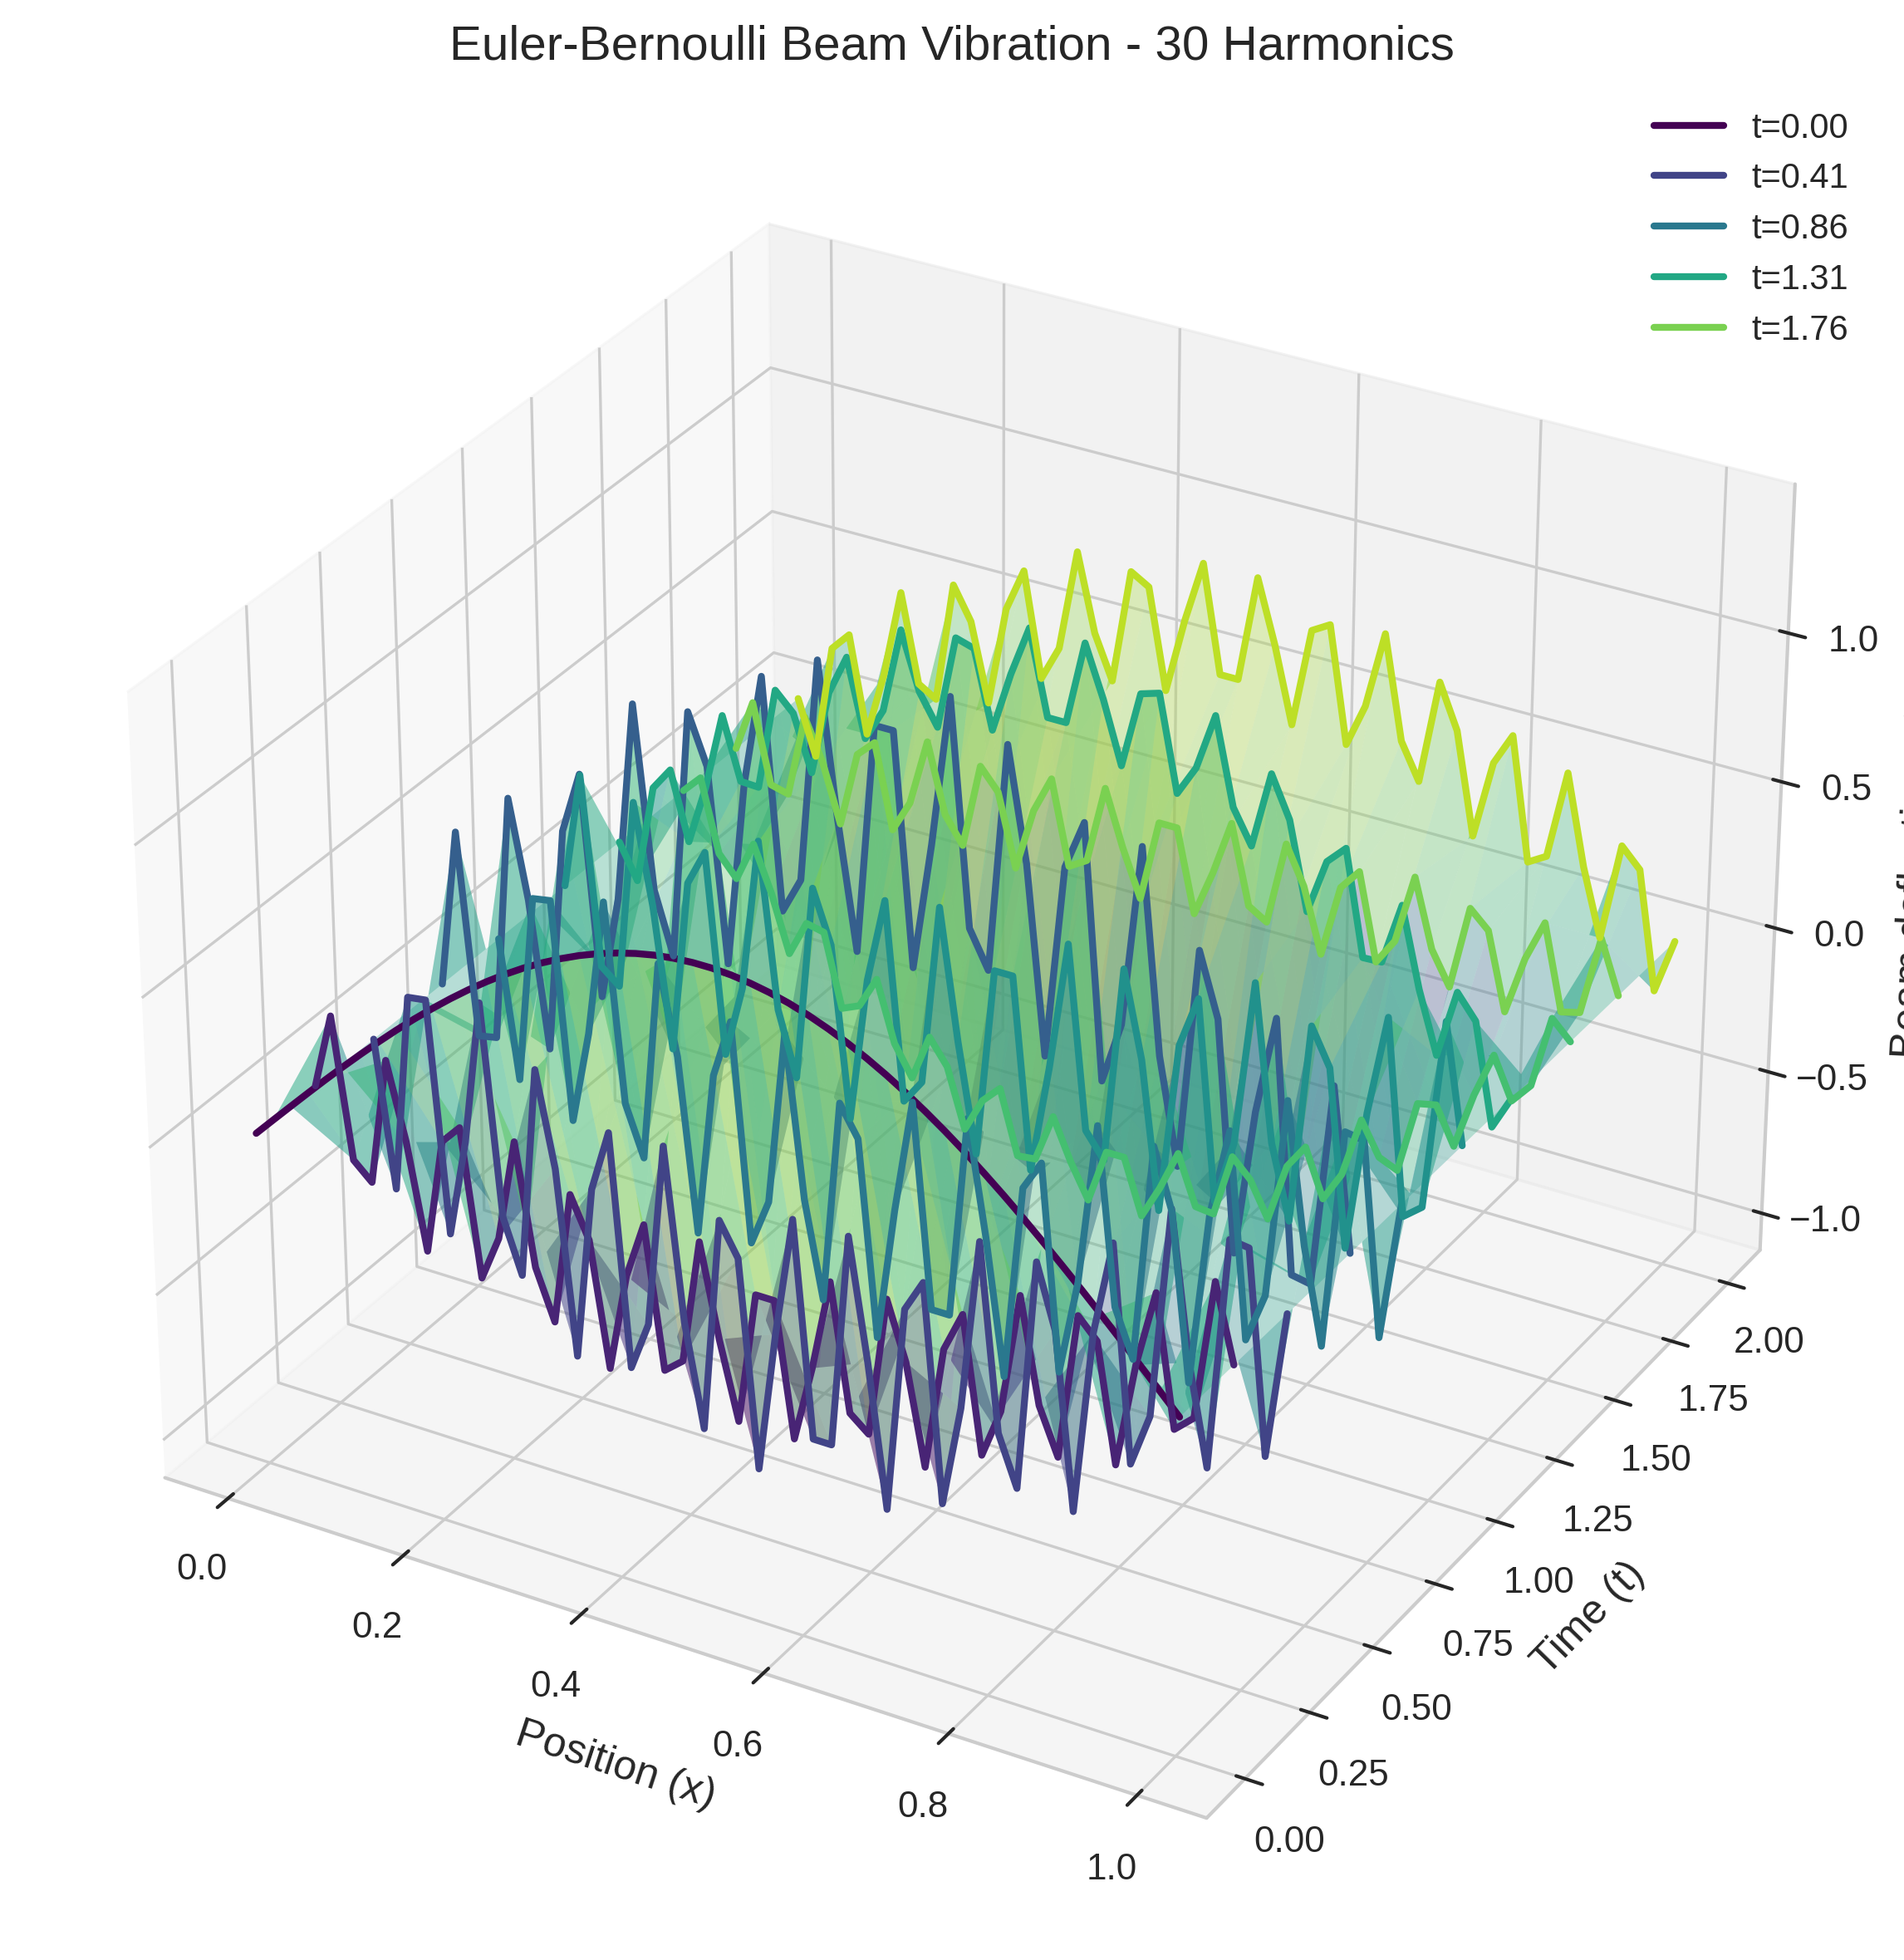
\includegraphics[width=0.9\linewidth]{figures/euler_bernoulli_3d_30h.png}
    \caption{Euler-Bernoulli beam vibration with 30 harmonics.}
    \label{fig:euler_30h}
\end{figure}

The figure presents the vibrational behavior of an Euler-Bernoulli beam reconstructed using 30 harmonics. The resulting surface plot reveals intricate waveforms and pronounced high-frequency oscillations, particularly evident at later time steps. These features indicate the inclusion of fine-scale vibrational modes that may be physically realistic in high-fidelity simulations but can introduce numerical instability or noise if not handled carefully. Although this level of harmonic detail provides a comprehensive representation of beam dynamics, it may exceed the necessary resolution for many practical applications. The spatial complexity introduces challenges in interpretation and may not contribute meaningfully to prediction accuracy, as suggested by rising error metrics beyond the optimal harmonic count. Thus, the 30-harmonic model demonstrates the limitations of overfitting in spectral decomposition, emphasizing that more modes do not always lead to better performance. This underscores the importance of harmonic selection based on problem-specific fidelity requirements.

\begin{figure}[t]
    \centering
    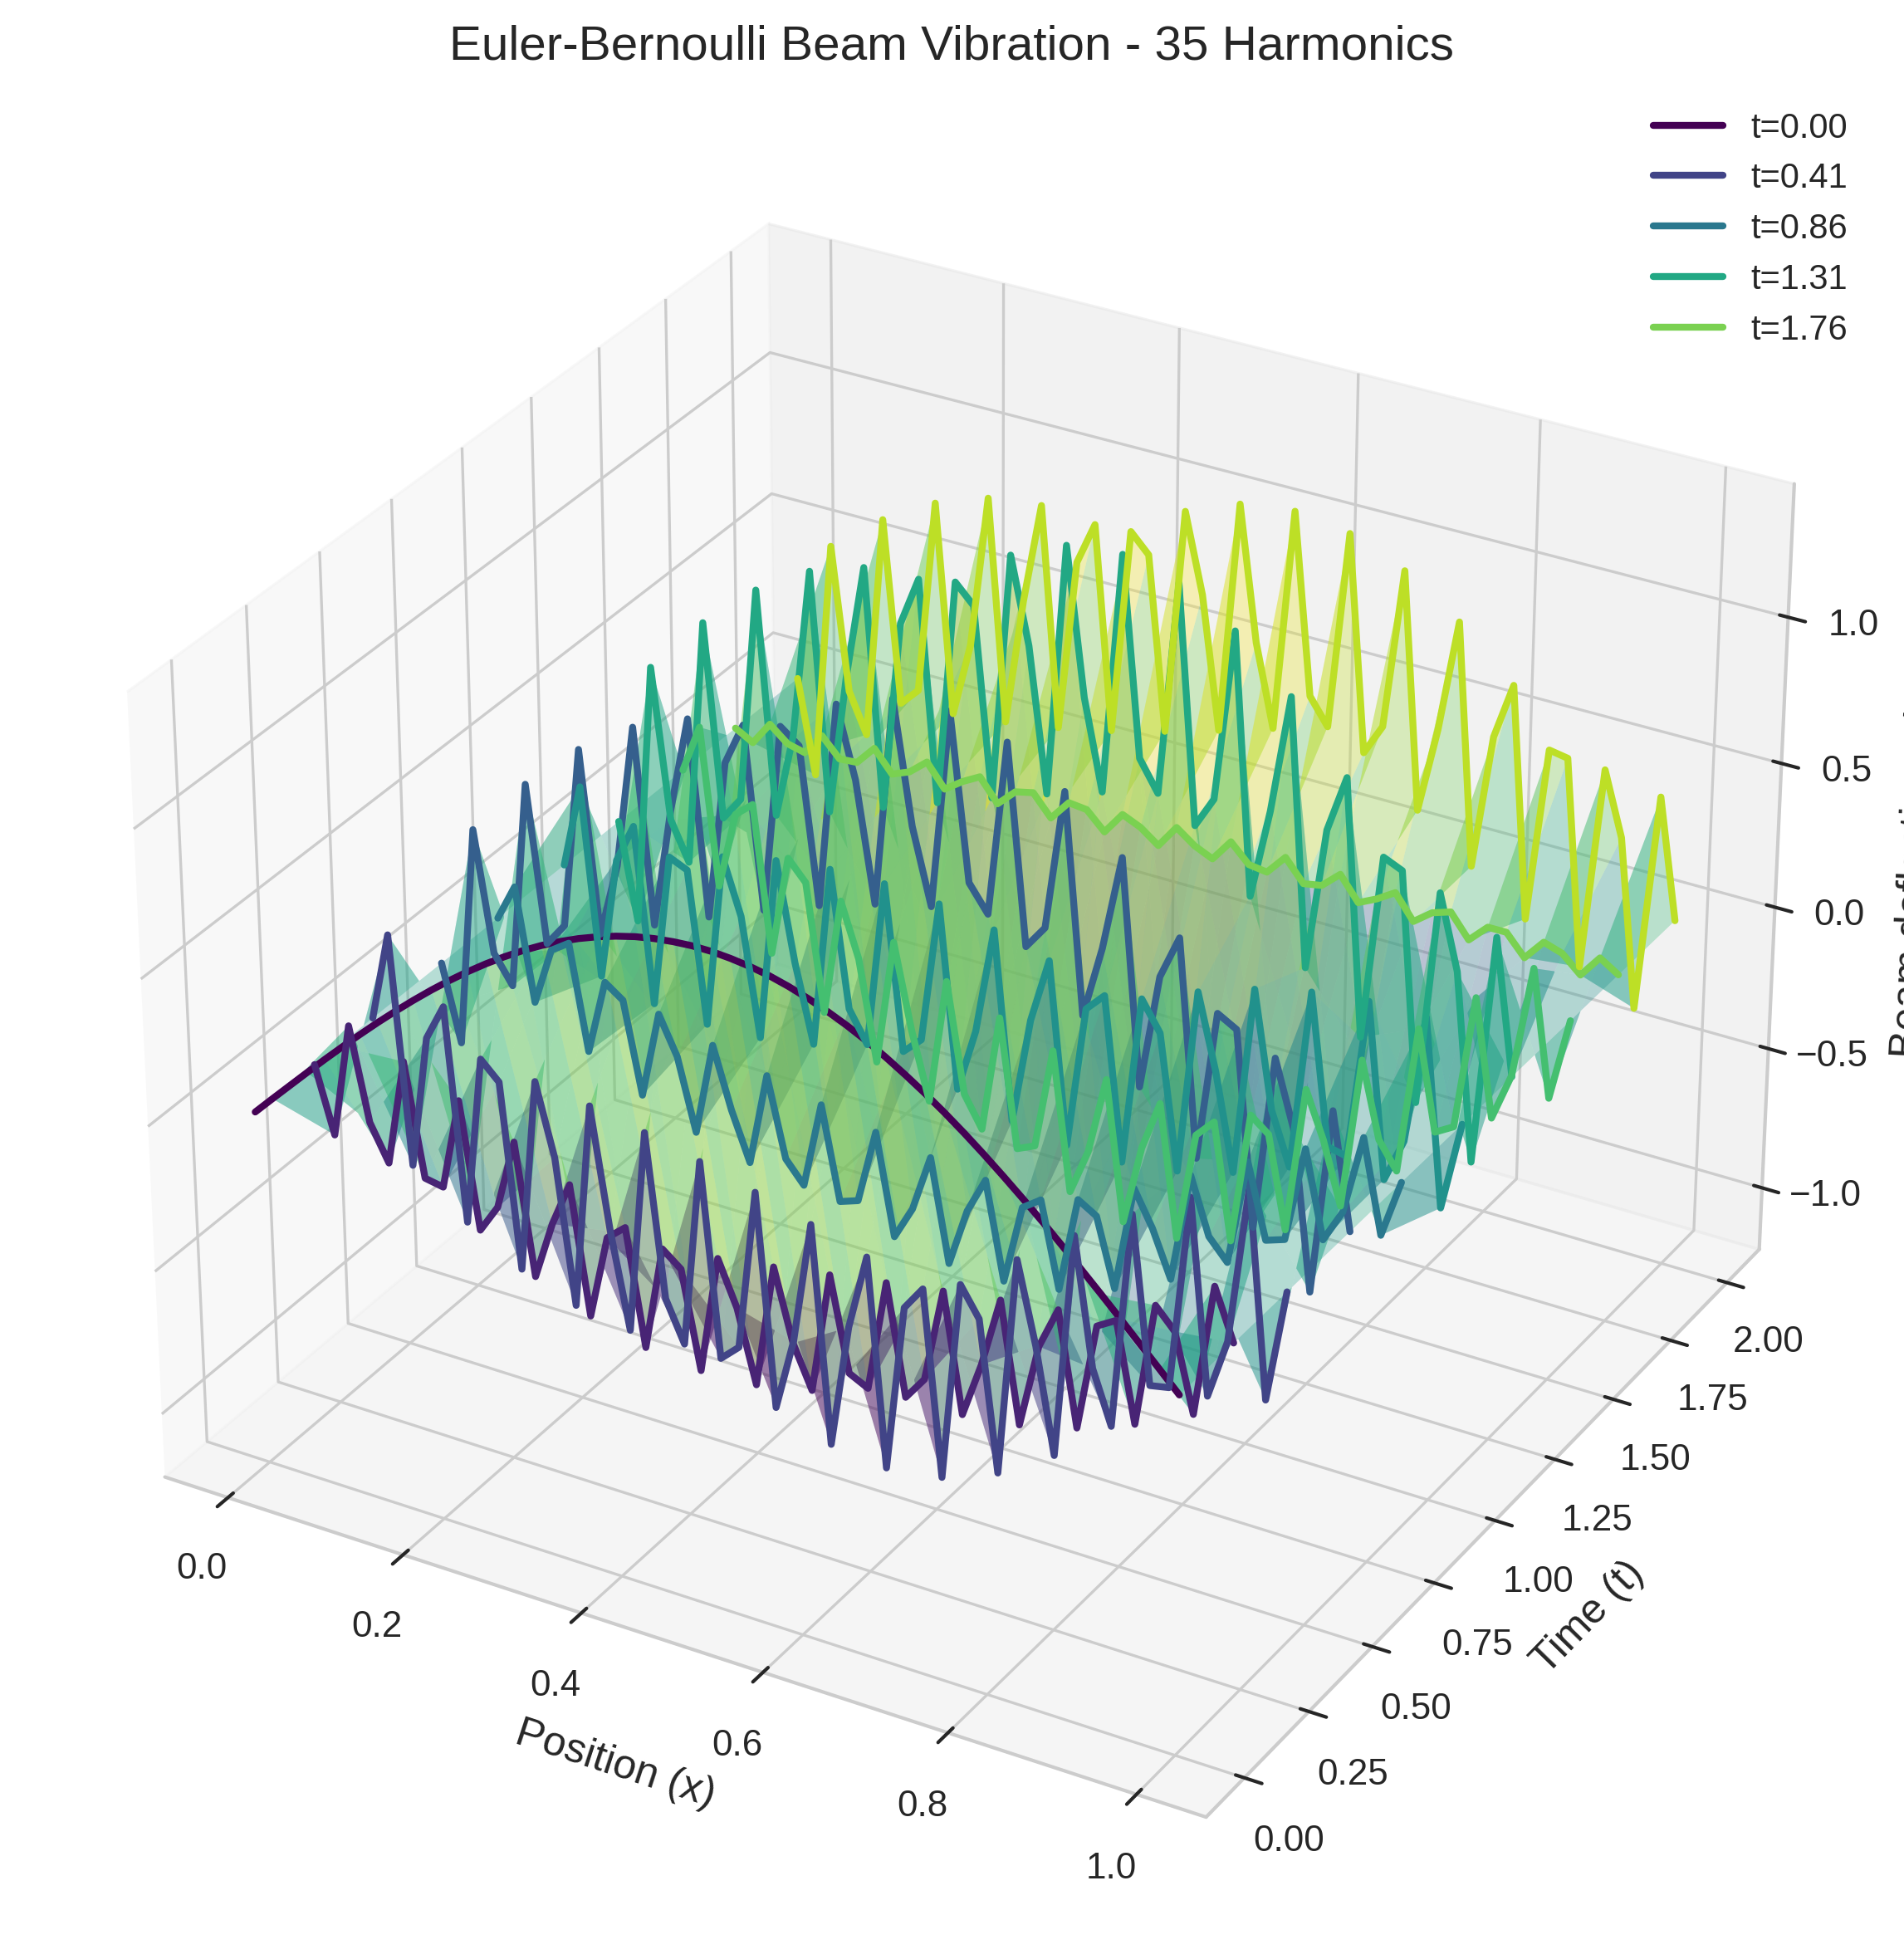
\includegraphics[width=0.9\linewidth]{figures/euler_bernoulli_3d_35h.png}
    \caption{Euler-Bernoulli beam vibration with 35 harmonics.}
    \label{fig:euler_35h}
\end{figure}

This figure visualizes the dynamic deflection of an Euler-Bernoulli beam using 35 harmonics. The waveform exhibits dense spatial oscillations, especially toward mid-span, reflecting the activation of high-frequency modes. While this harmonic resolution captures intricate details of the beam’s vibrational profile, the benefit in accuracy becomes marginal compared to configurations with fewer harmonics. Instead, the increase in numerical noise and model complexity becomes more apparent. Such fine modal components may not contribute significantly to energy transmission but can obscure meaningful mechanical behavior and increase computational costs. This reinforces that there is an optimal level of spectral resolution, beyond which additional harmonics yield diminishing returns. Hence, although the 35-harmonic model provides rich spatial detail, it may introduce overfitting or instability in simulations where simpler models are sufficient.

\begin{figure}[t]
    \centering
    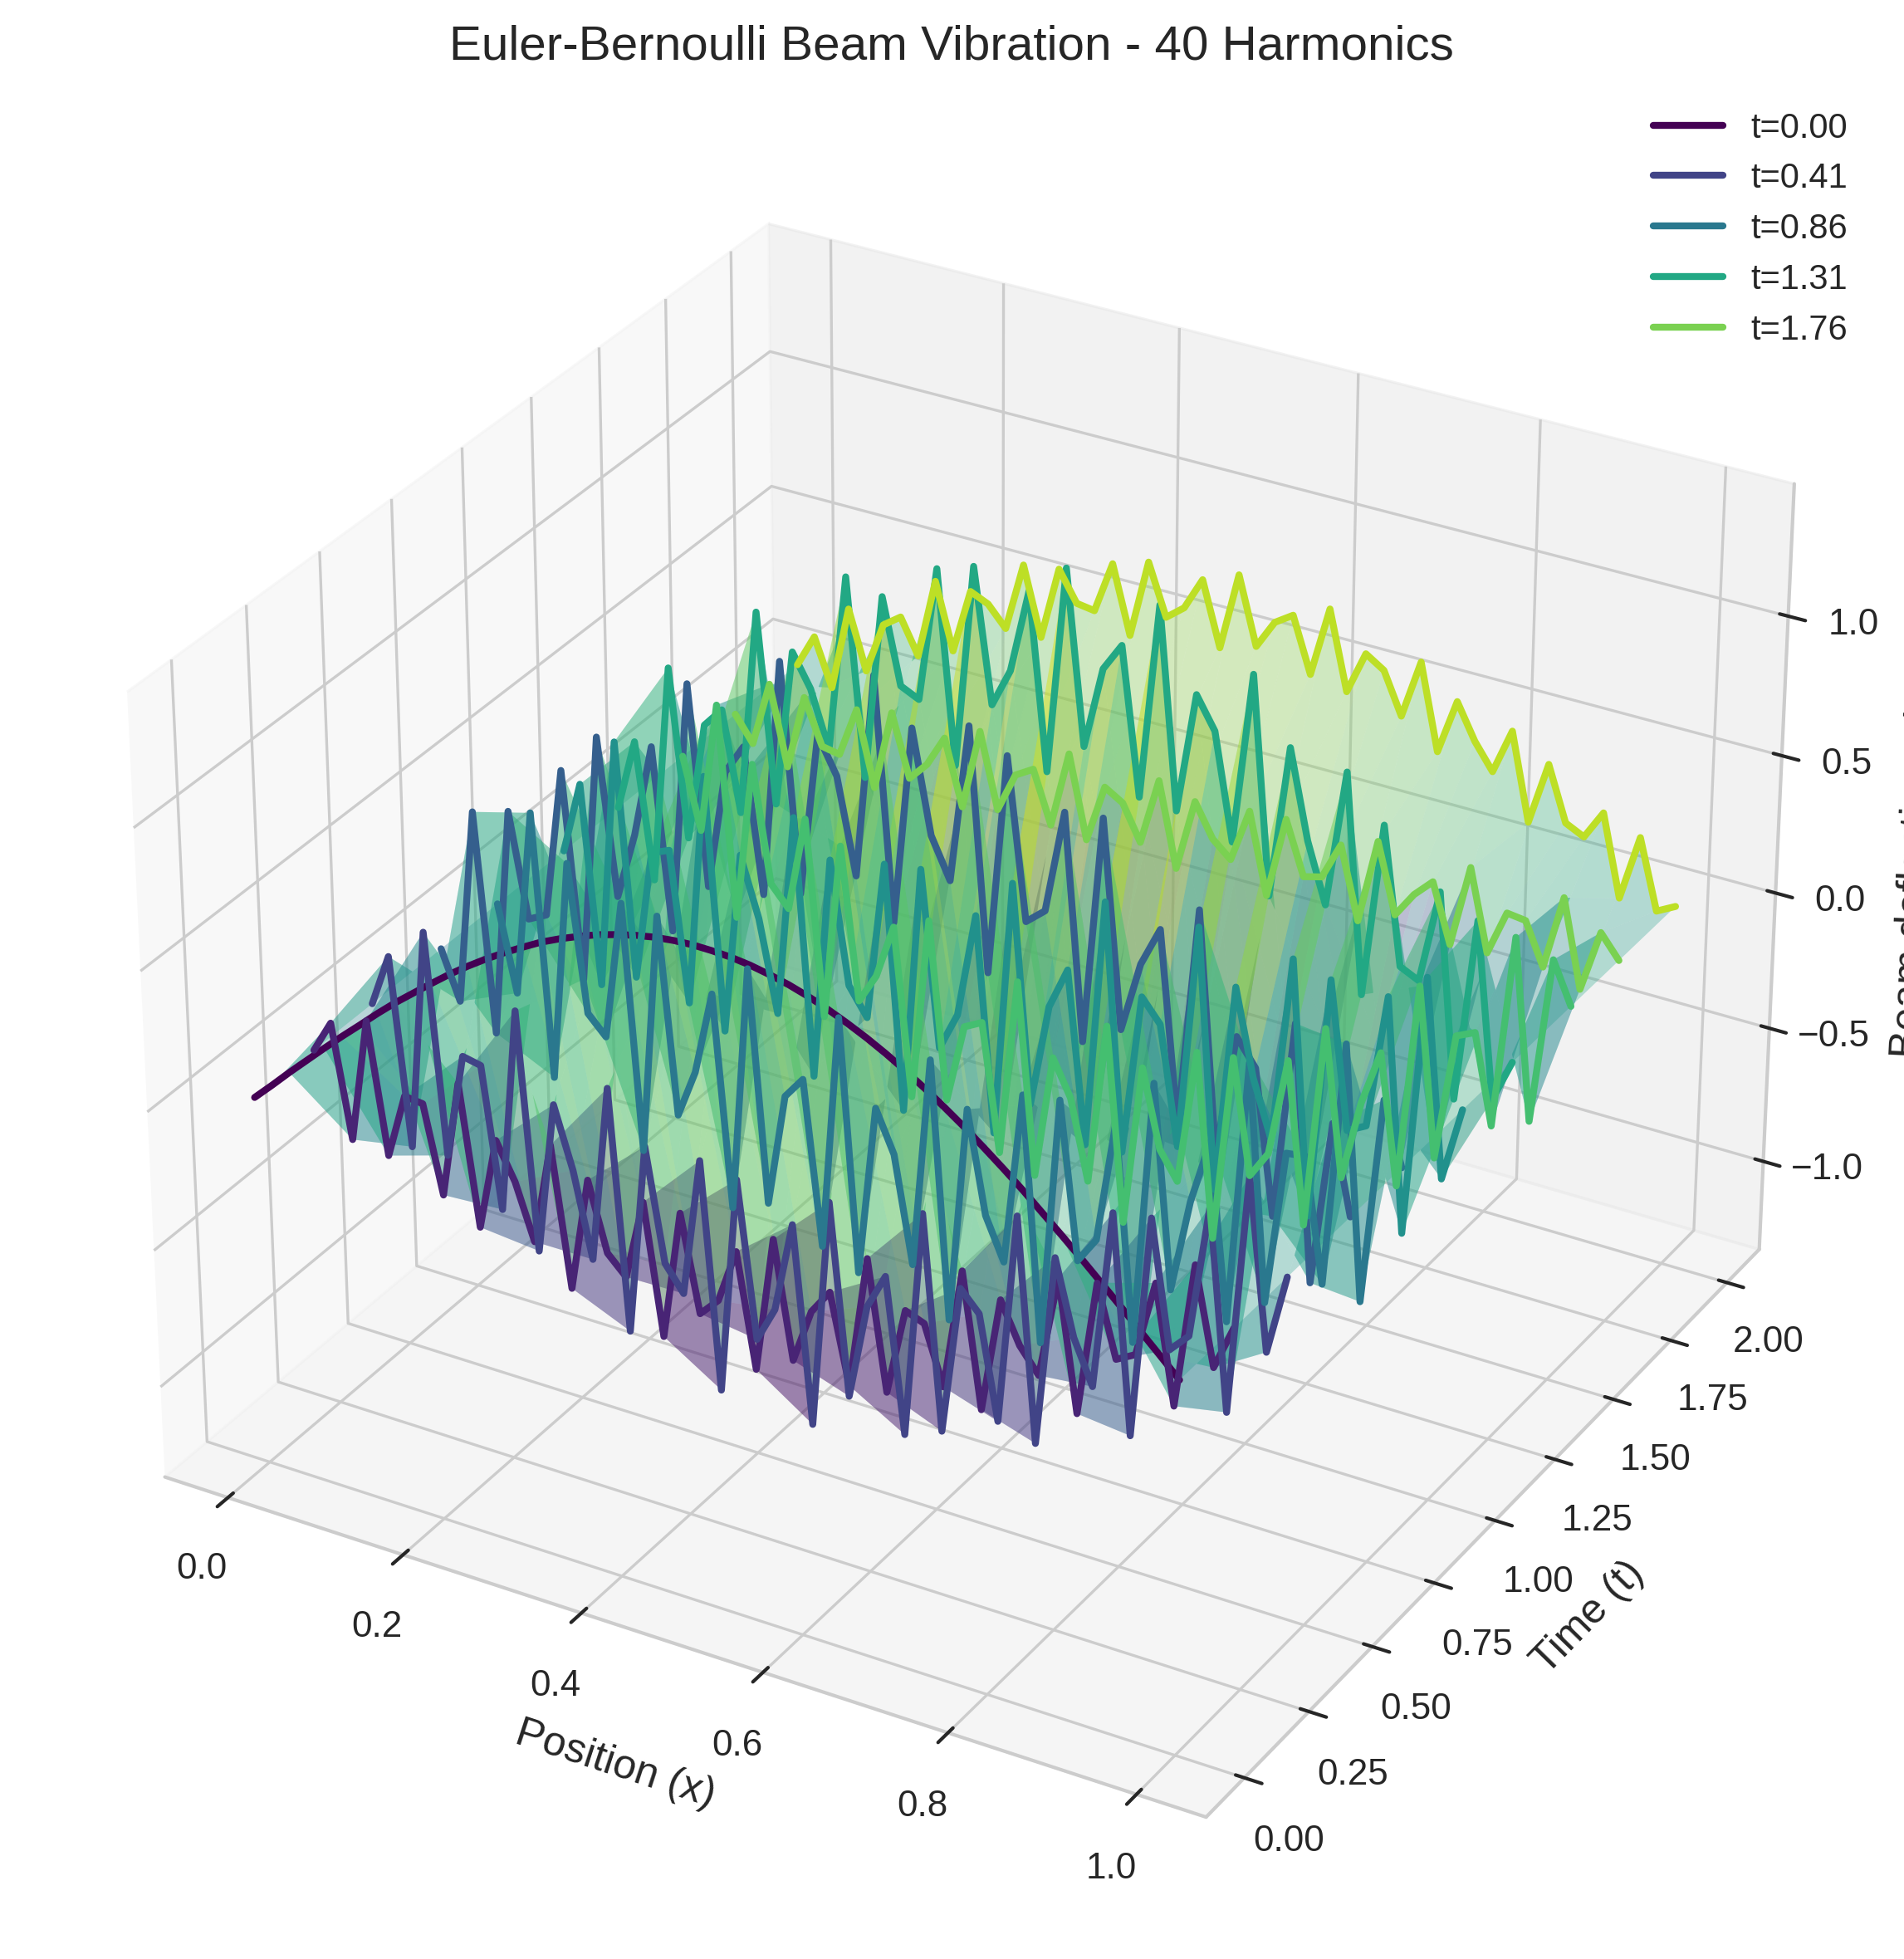
\includegraphics[width=0.9\linewidth]{figures/euler_bernoulli_3d_40h.png}
    \caption{Euler-Bernoulli beam vibration with 40 harmonics.}
    \label{fig:euler_40h}
\end{figure}

This figure illustrates Euler-Bernoulli beam dynamics reconstructed with 40 harmonics. The response surface is characterized by extremely fine-grained oscillations, particularly along the beam’s central region and near boundary layers. These features result from the contribution of high-frequency harmonics, which can overrepresent minor vibrational modes. Despite capturing high-resolution dynamics, the model's added complexity does not translate into improved predictive performance—often leading to greater numerical error and instability. The presence of spurious patterns or artificial sharp peaks suggests potential overfitting to high-frequency noise. While such models may be useful in academic settings for studying high-mode interactions, they are generally inefficient for practical structural dynamics tasks. This example demonstrates the risks of excessive harmonic decomposition in spectral modeling of mechanical systems.

\begin{figure}[t]
    \centering
    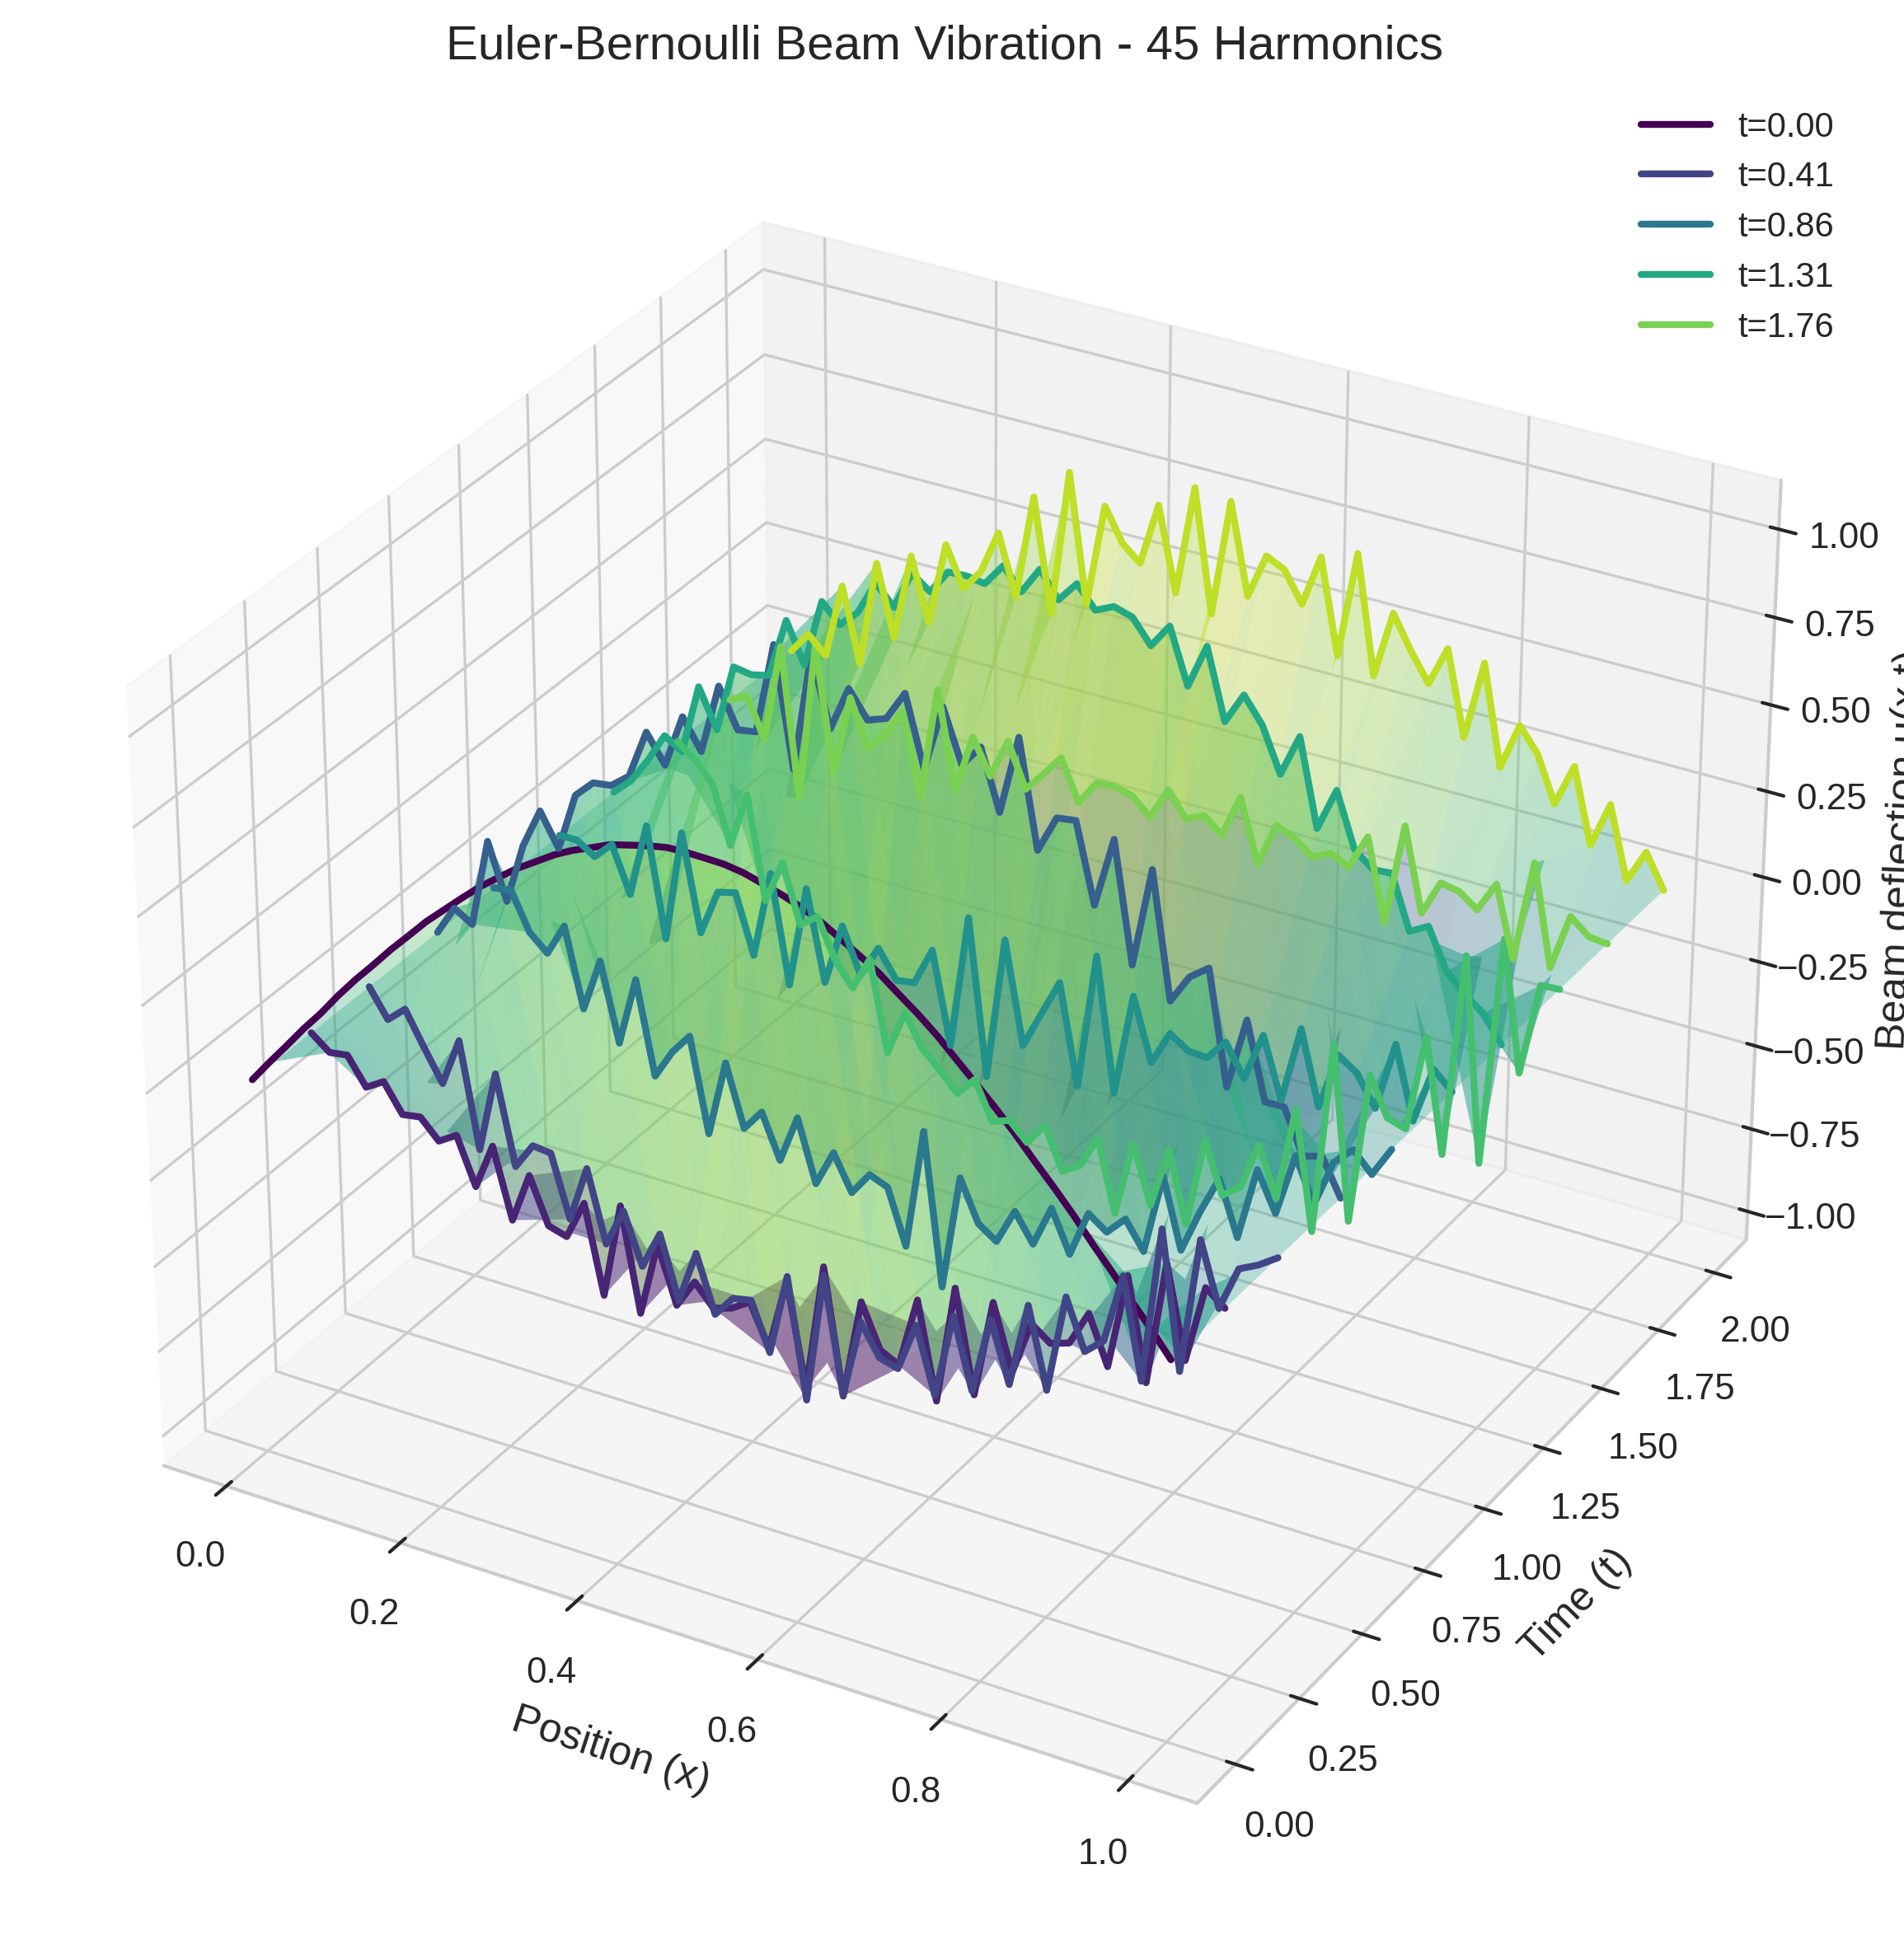
\includegraphics[width=0.9\linewidth]{figures/euler_bernoulli_3d_45h.png}
    \caption{Euler-Bernoulli beam vibration with 45 harmonics.}
    \label{fig:euler_45h}
\end{figure}

The vibration surface shown in this figure corresponds to a 45-harmonic approximation of an Euler-Bernoulli beam. At this harmonic density, the model introduces an overload of high-frequency content, which overshadows the beam’s fundamental deflection profile. While the spatial and temporal resolution is extremely detailed, the waveform loses physical interpretability, showing rapid, jagged transitions that are not characteristic of real mechanical vibrations. This is a hallmark of overfitting in spectral models, where the system captures numerical artifacts rather than physically relevant modes. Consequently, although the 45-harmonic simulation is technically more resolved, it performs worse on standard error metrics and is less reliable in engineering design contexts. This result emphasizes that more harmonics can degrade model utility when noise dominates over meaningful signals.

\begin{figure}[t]
    \centering
    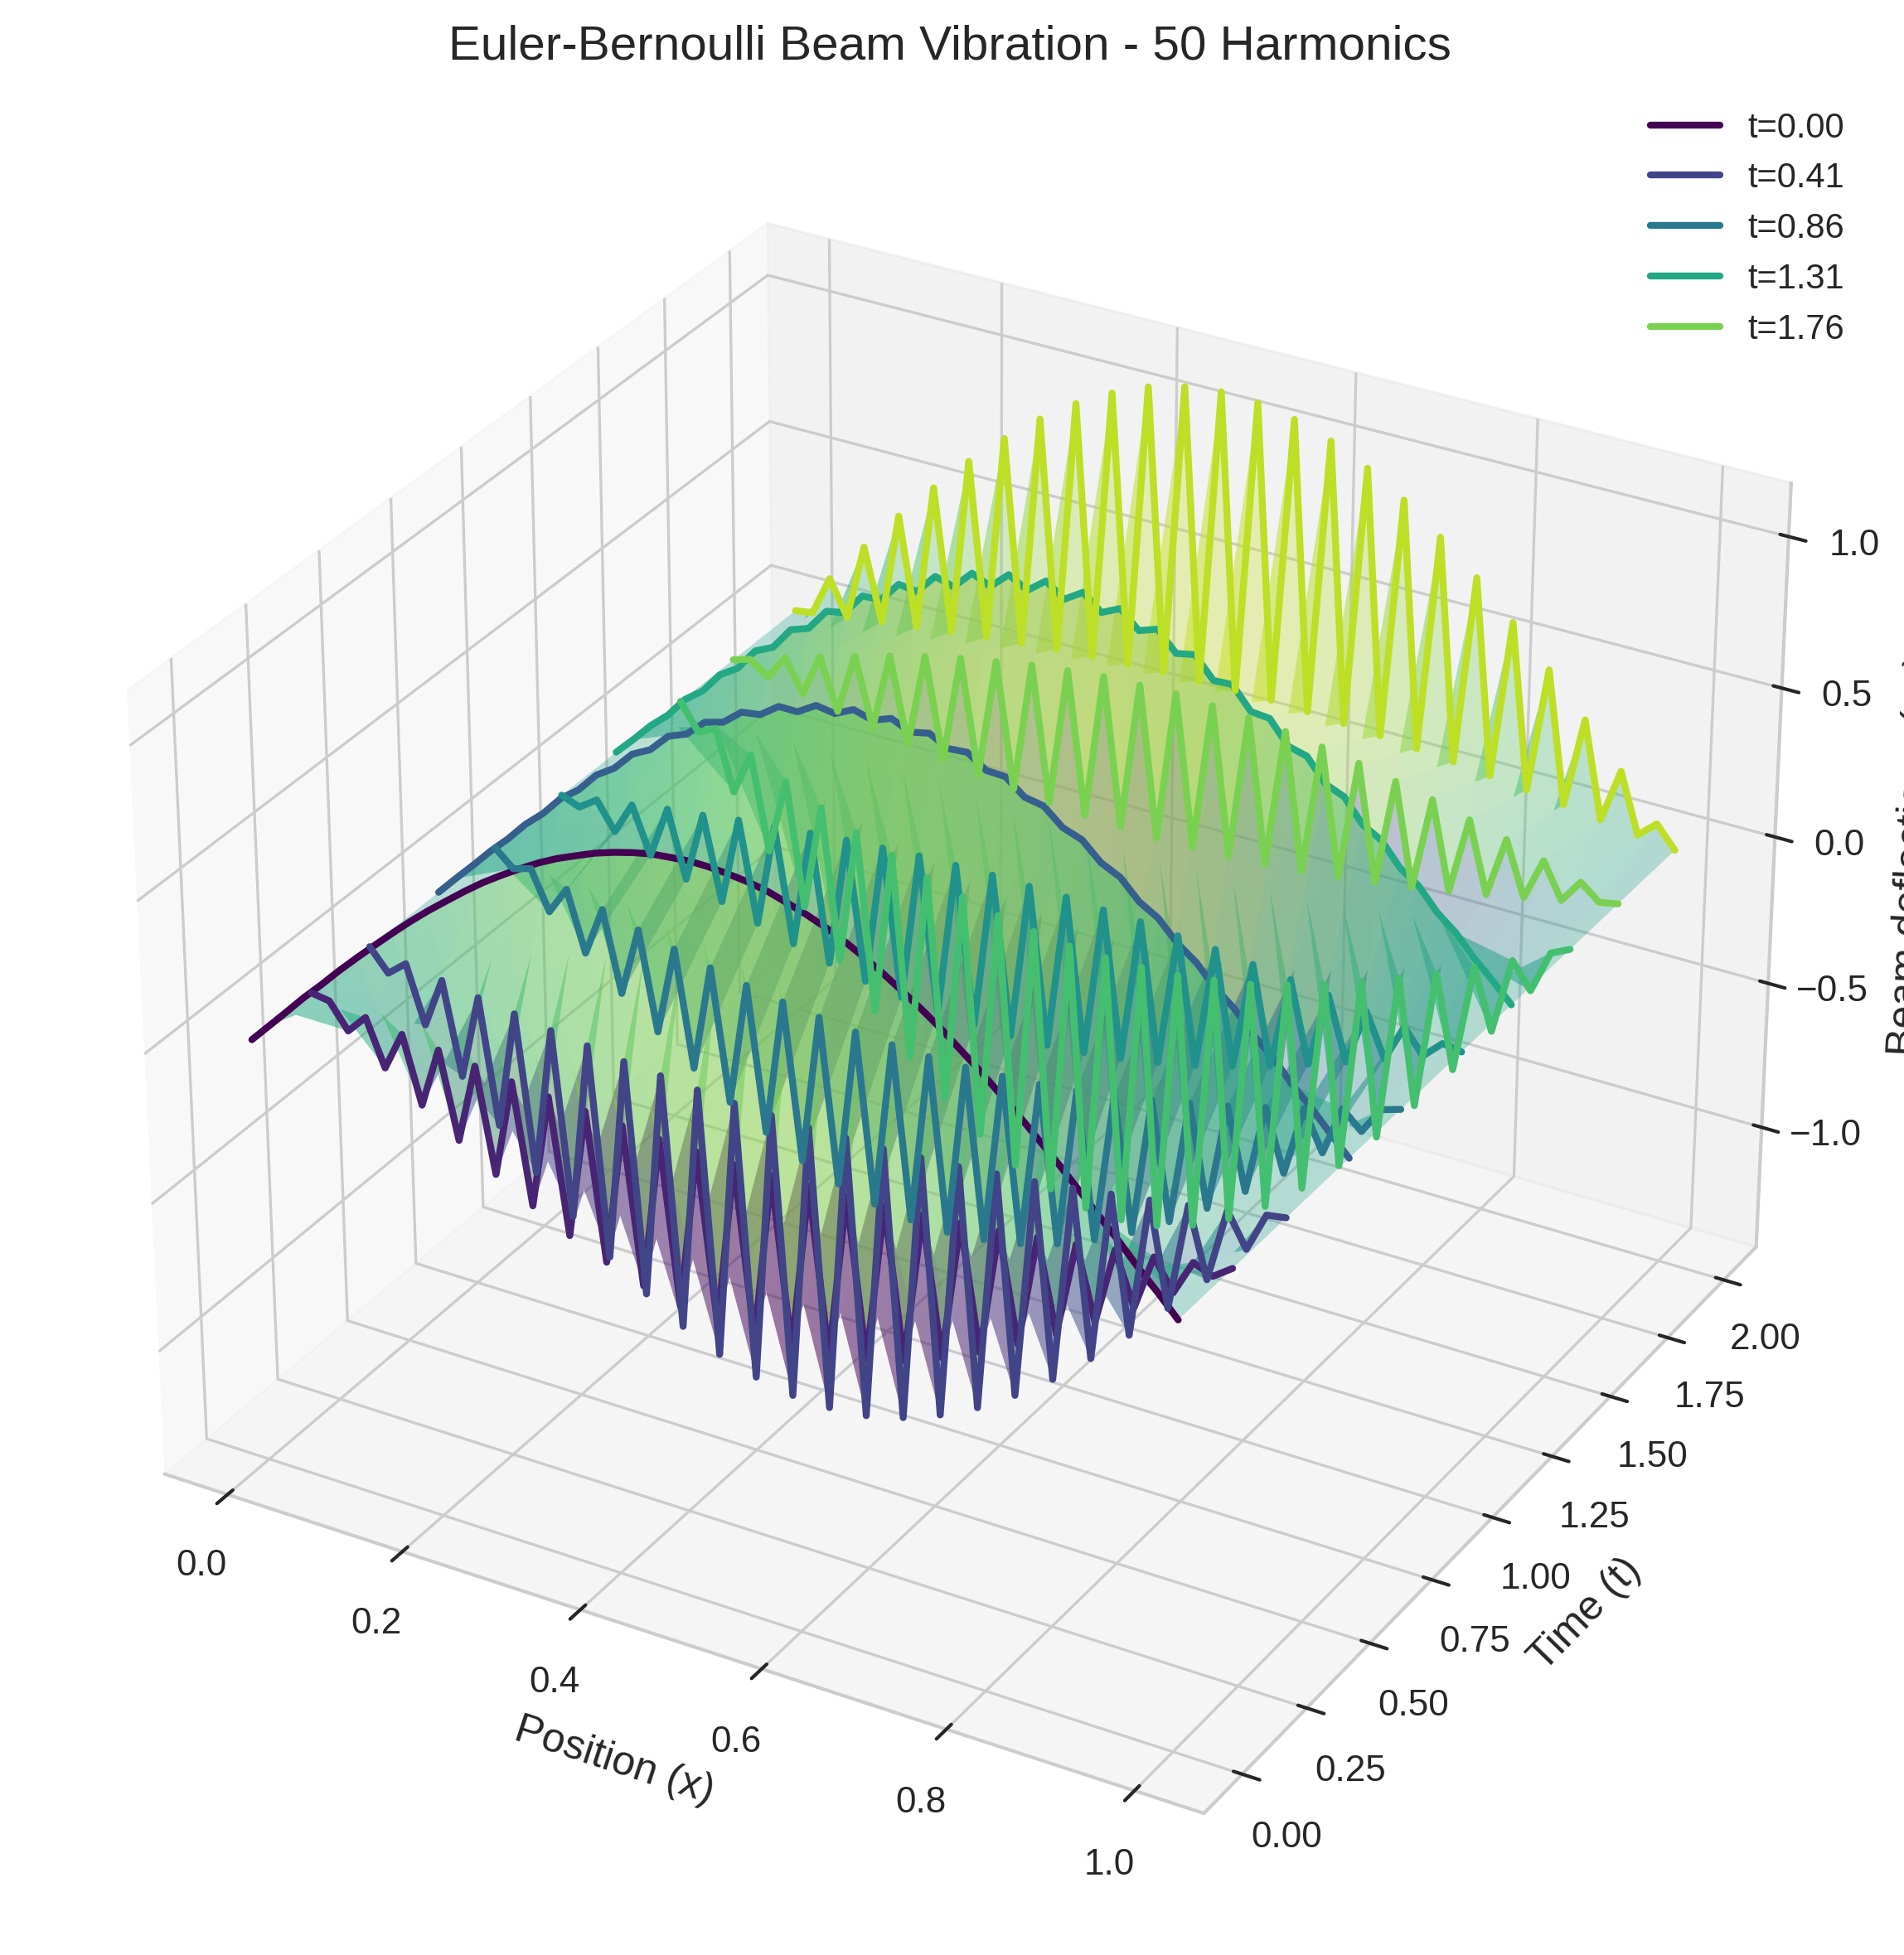
\includegraphics[width=0.9\linewidth]{figures/euler_bernoulli_3d_50h.png}
    \caption{Euler-Bernoulli beam vibration with 50 harmonics.}
    \label{fig:euler_50h}
\end{figure}

This plot shows the Euler-Bernoulli beam’s vibration reconstructed with 50 harmonics—the highest considered resolution in this study. The model yields a highly oscillatory surface with prominent, densely packed wave patterns along the beam's length. These extreme fluctuations, while mathematically consistent with high harmonic content, are physically unrealistic for typical beam responses under small deflection assumptions. Moreover, the error metrics (as seen in comparison plots) confirm that accuracy does not improve with this harmonic density; instead, it degrades due to numerical noise and overfitting. The 50-harmonic model highlights the limitations of brute-force spectral expansion, suggesting that truncating to an optimal number of harmonics—such as 10 to 15—can yield better fidelity with reduced computational and interpretive cost. This figure serves as a clear example of the trade-off between resolution and model robustness in vibrational analyses.

\begin{figure}[t]
    \centering
    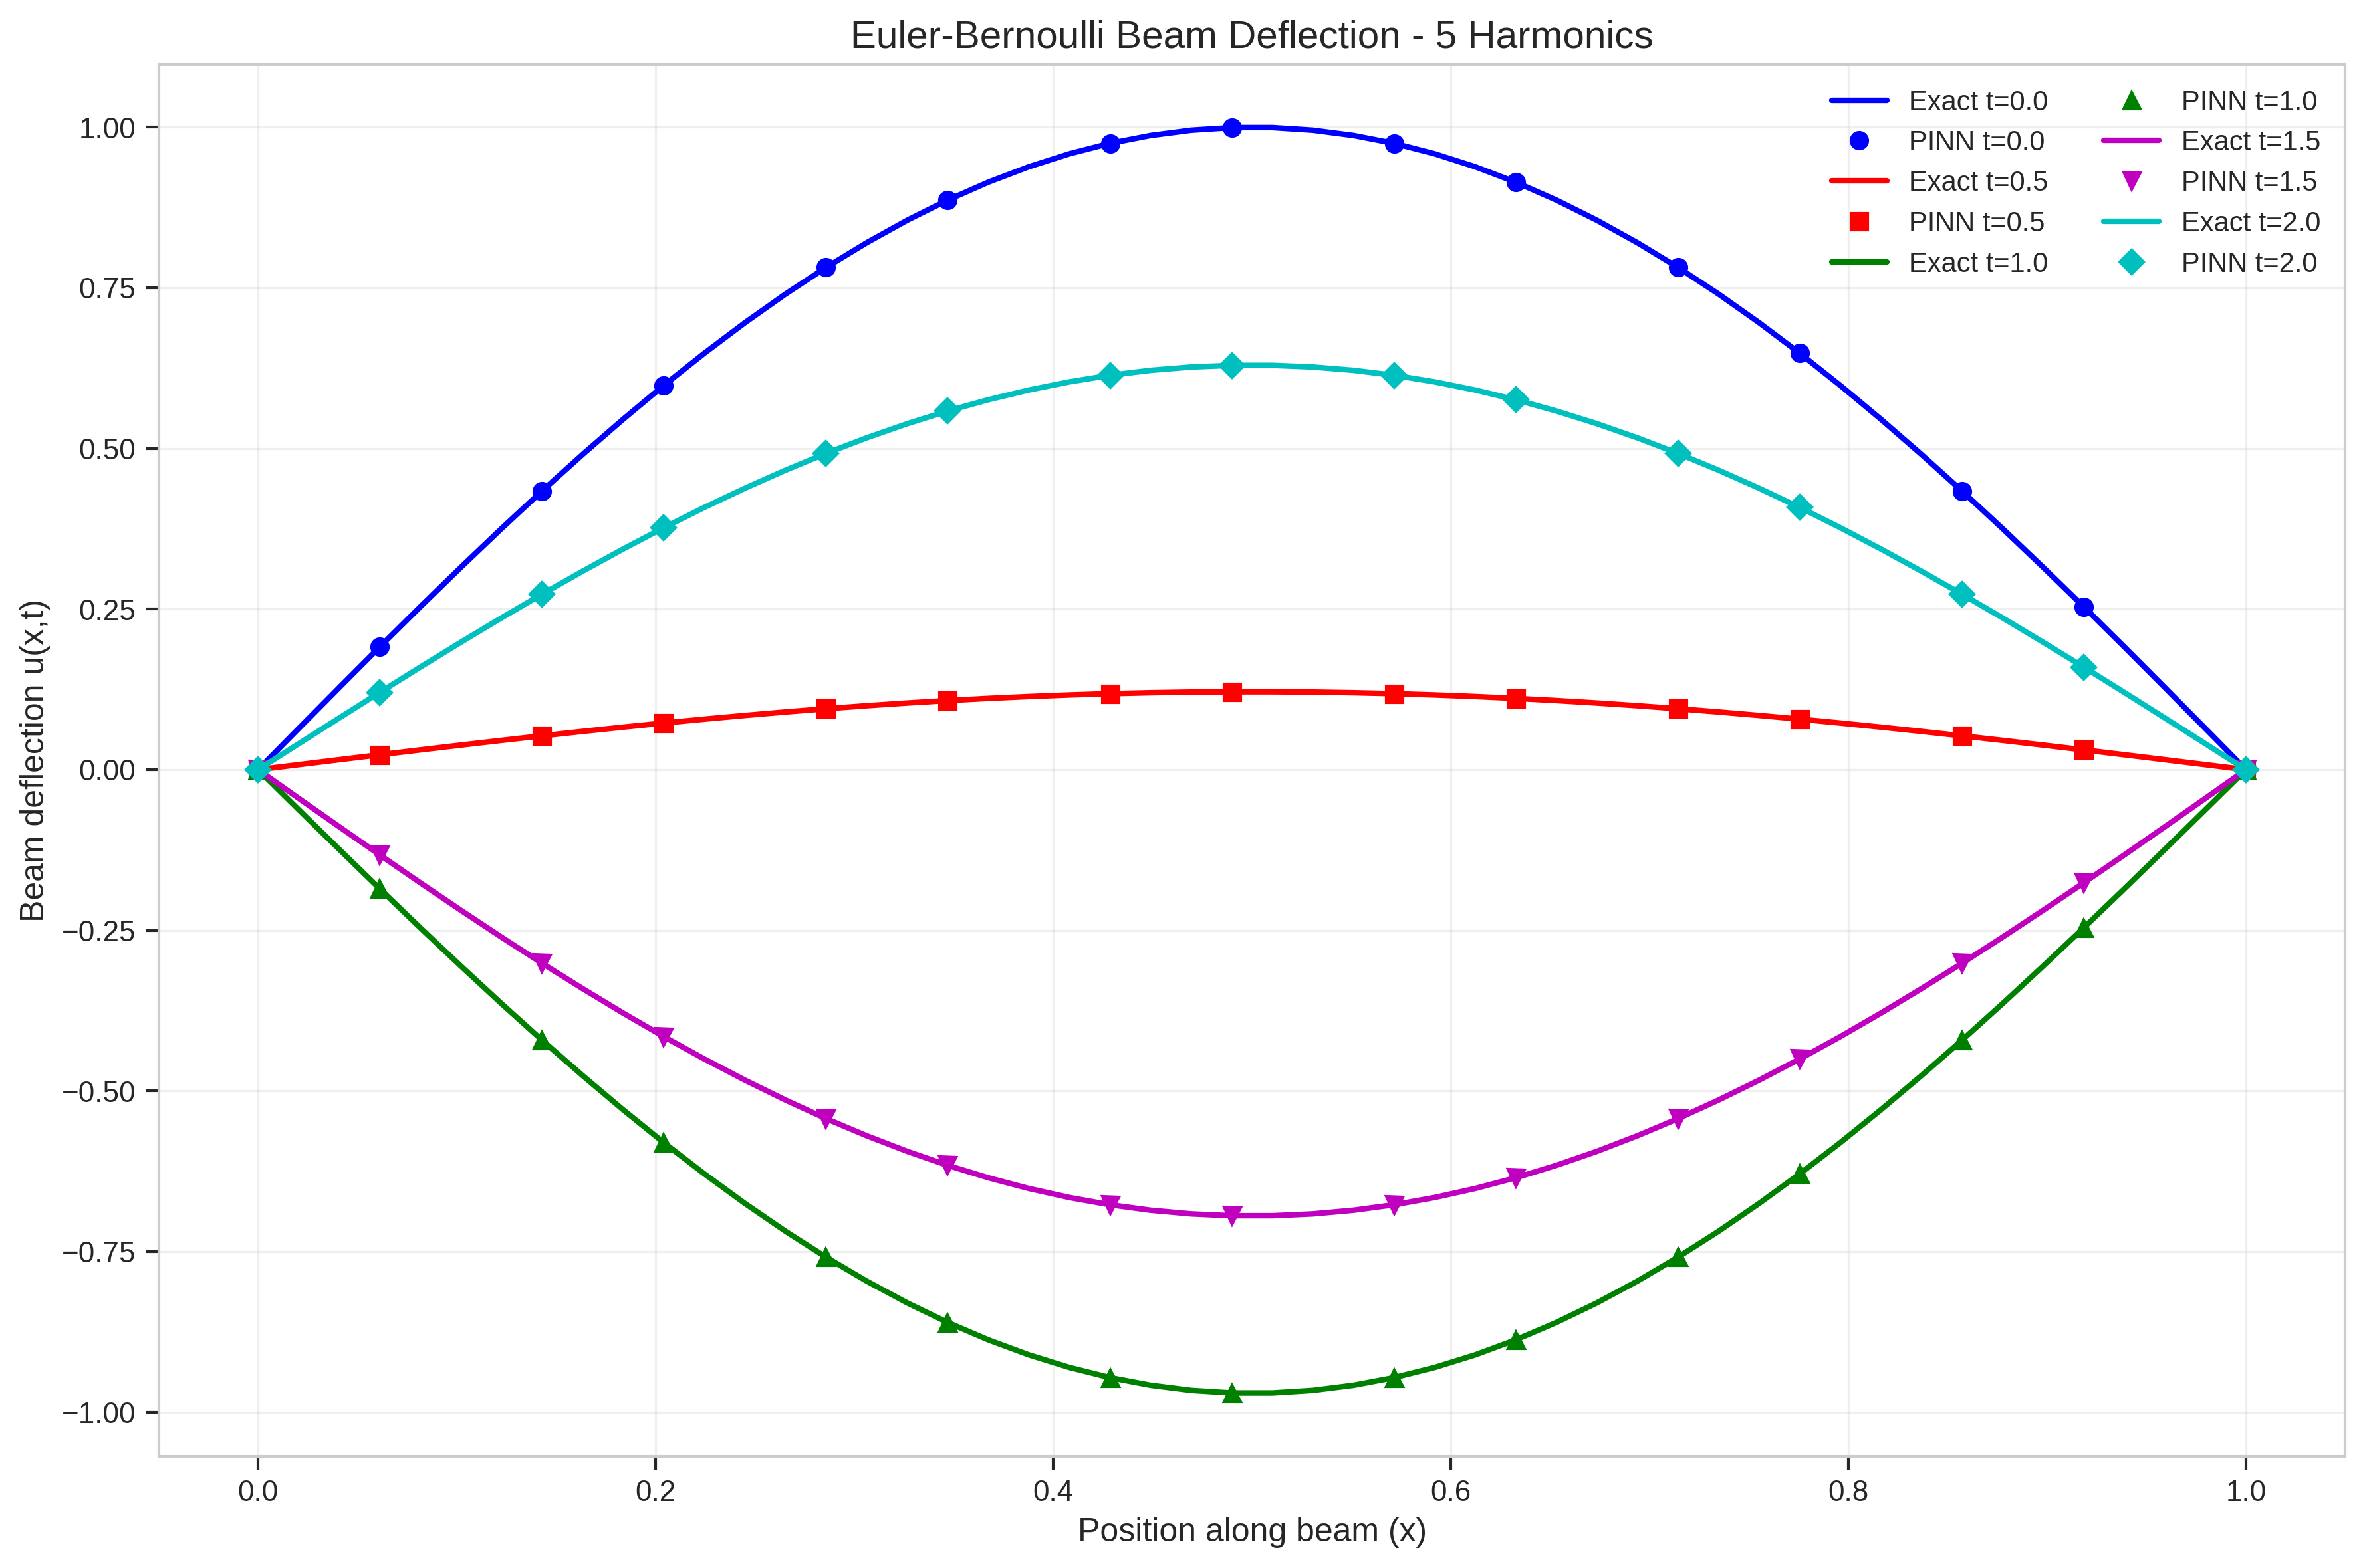
\includegraphics[width=0.9\linewidth]{figures/euler_bernoulli_beam_5h.png}
    \caption{Euler-Bernoulli beam dynamics modeled with 5 harmonics.}
    \label{fig:euler_bernoulli_beam_5h}
\end{figure}

Figure~\ref{fig:euler_bernoulli_beam_5h} presents the beam deflection computed using just 5 harmonics. Despite the low harmonic count, the model retains the global structure of the beam’s motion and captures the first few dominant vibration modes effectively. The deflection curves are smooth and stable across time, with minimal deviation between exact and PINN predictions. However, finer details—especially near $x=0.5$—are lost, leading to slightly underfit dynamics at mid-span. This under-parameterization trades accuracy for robustness, yielding consistent but less expressive behavior. While this model excels in generalization and computational efficiency, it is less suitable when high-fidelity resolution of dynamic features is needed. Nonetheless, for coarse-grained modeling or scenarios with limited computational resources, the 5-harmonic configuration offers a viable, lightweight alternative.

\begin{figure}[t]
    \centering
    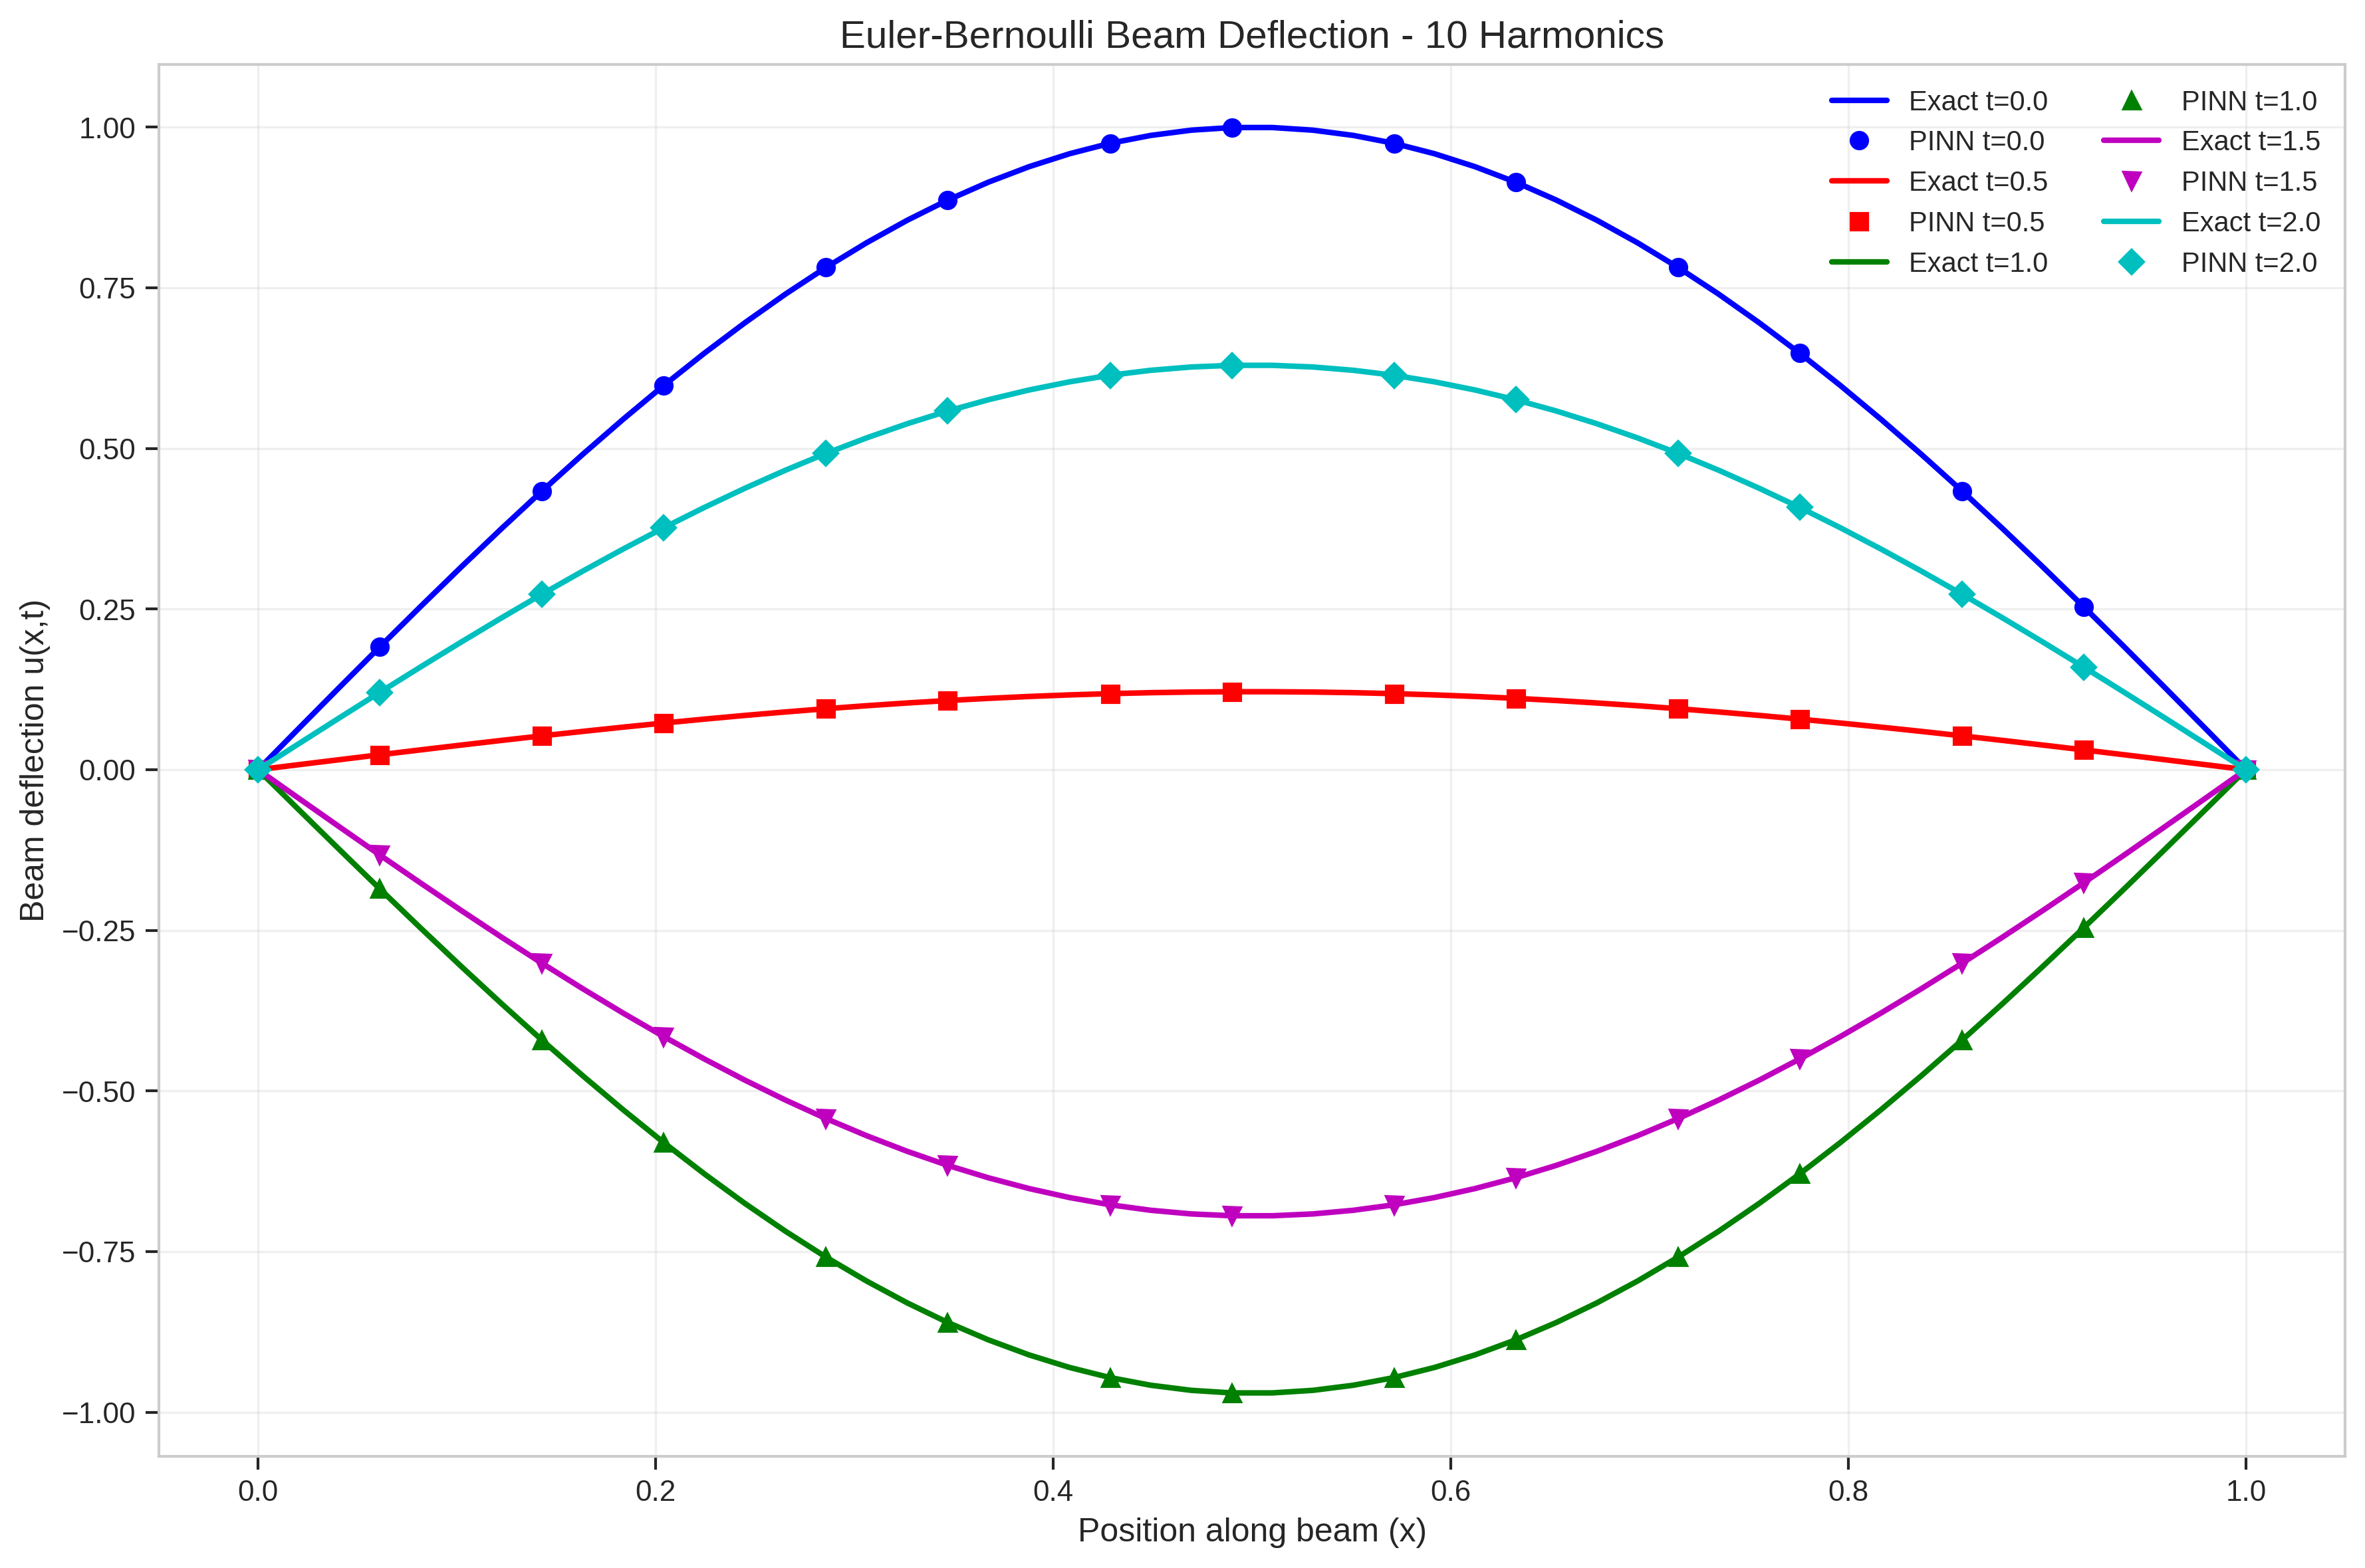
\includegraphics[width=0.9\linewidth]{figures/euler_bernoulli_beam_10h.png}
    \caption{Euler-Bernoulli Beam Deflection using 10 Harmonics.}
    \label{fig:beam_deflection_10h}
\end{figure}

Using 10 harmonics yields a highly stable and accurate solution. The exact deflection curves are smooth and physically realistic, and the PINN predictions show close alignment across all time steps. Unlike higher harmonic cases, no significant deviations or instability are observed. The balance between expressiveness and generalization is optimal here—sufficient detail to resolve the primary modes of vibration, but not so many harmonics that the PINN overfits noise. This result supports 10 harmonics as a sweet spot: it captures the essential physics of the Euler-Bernoulli beam while maintaining numerical efficiency and model robustness. It also suggests that further increasing harmonic count may not justify the additional complexity.

\begin{figure}[t]
    \centering
    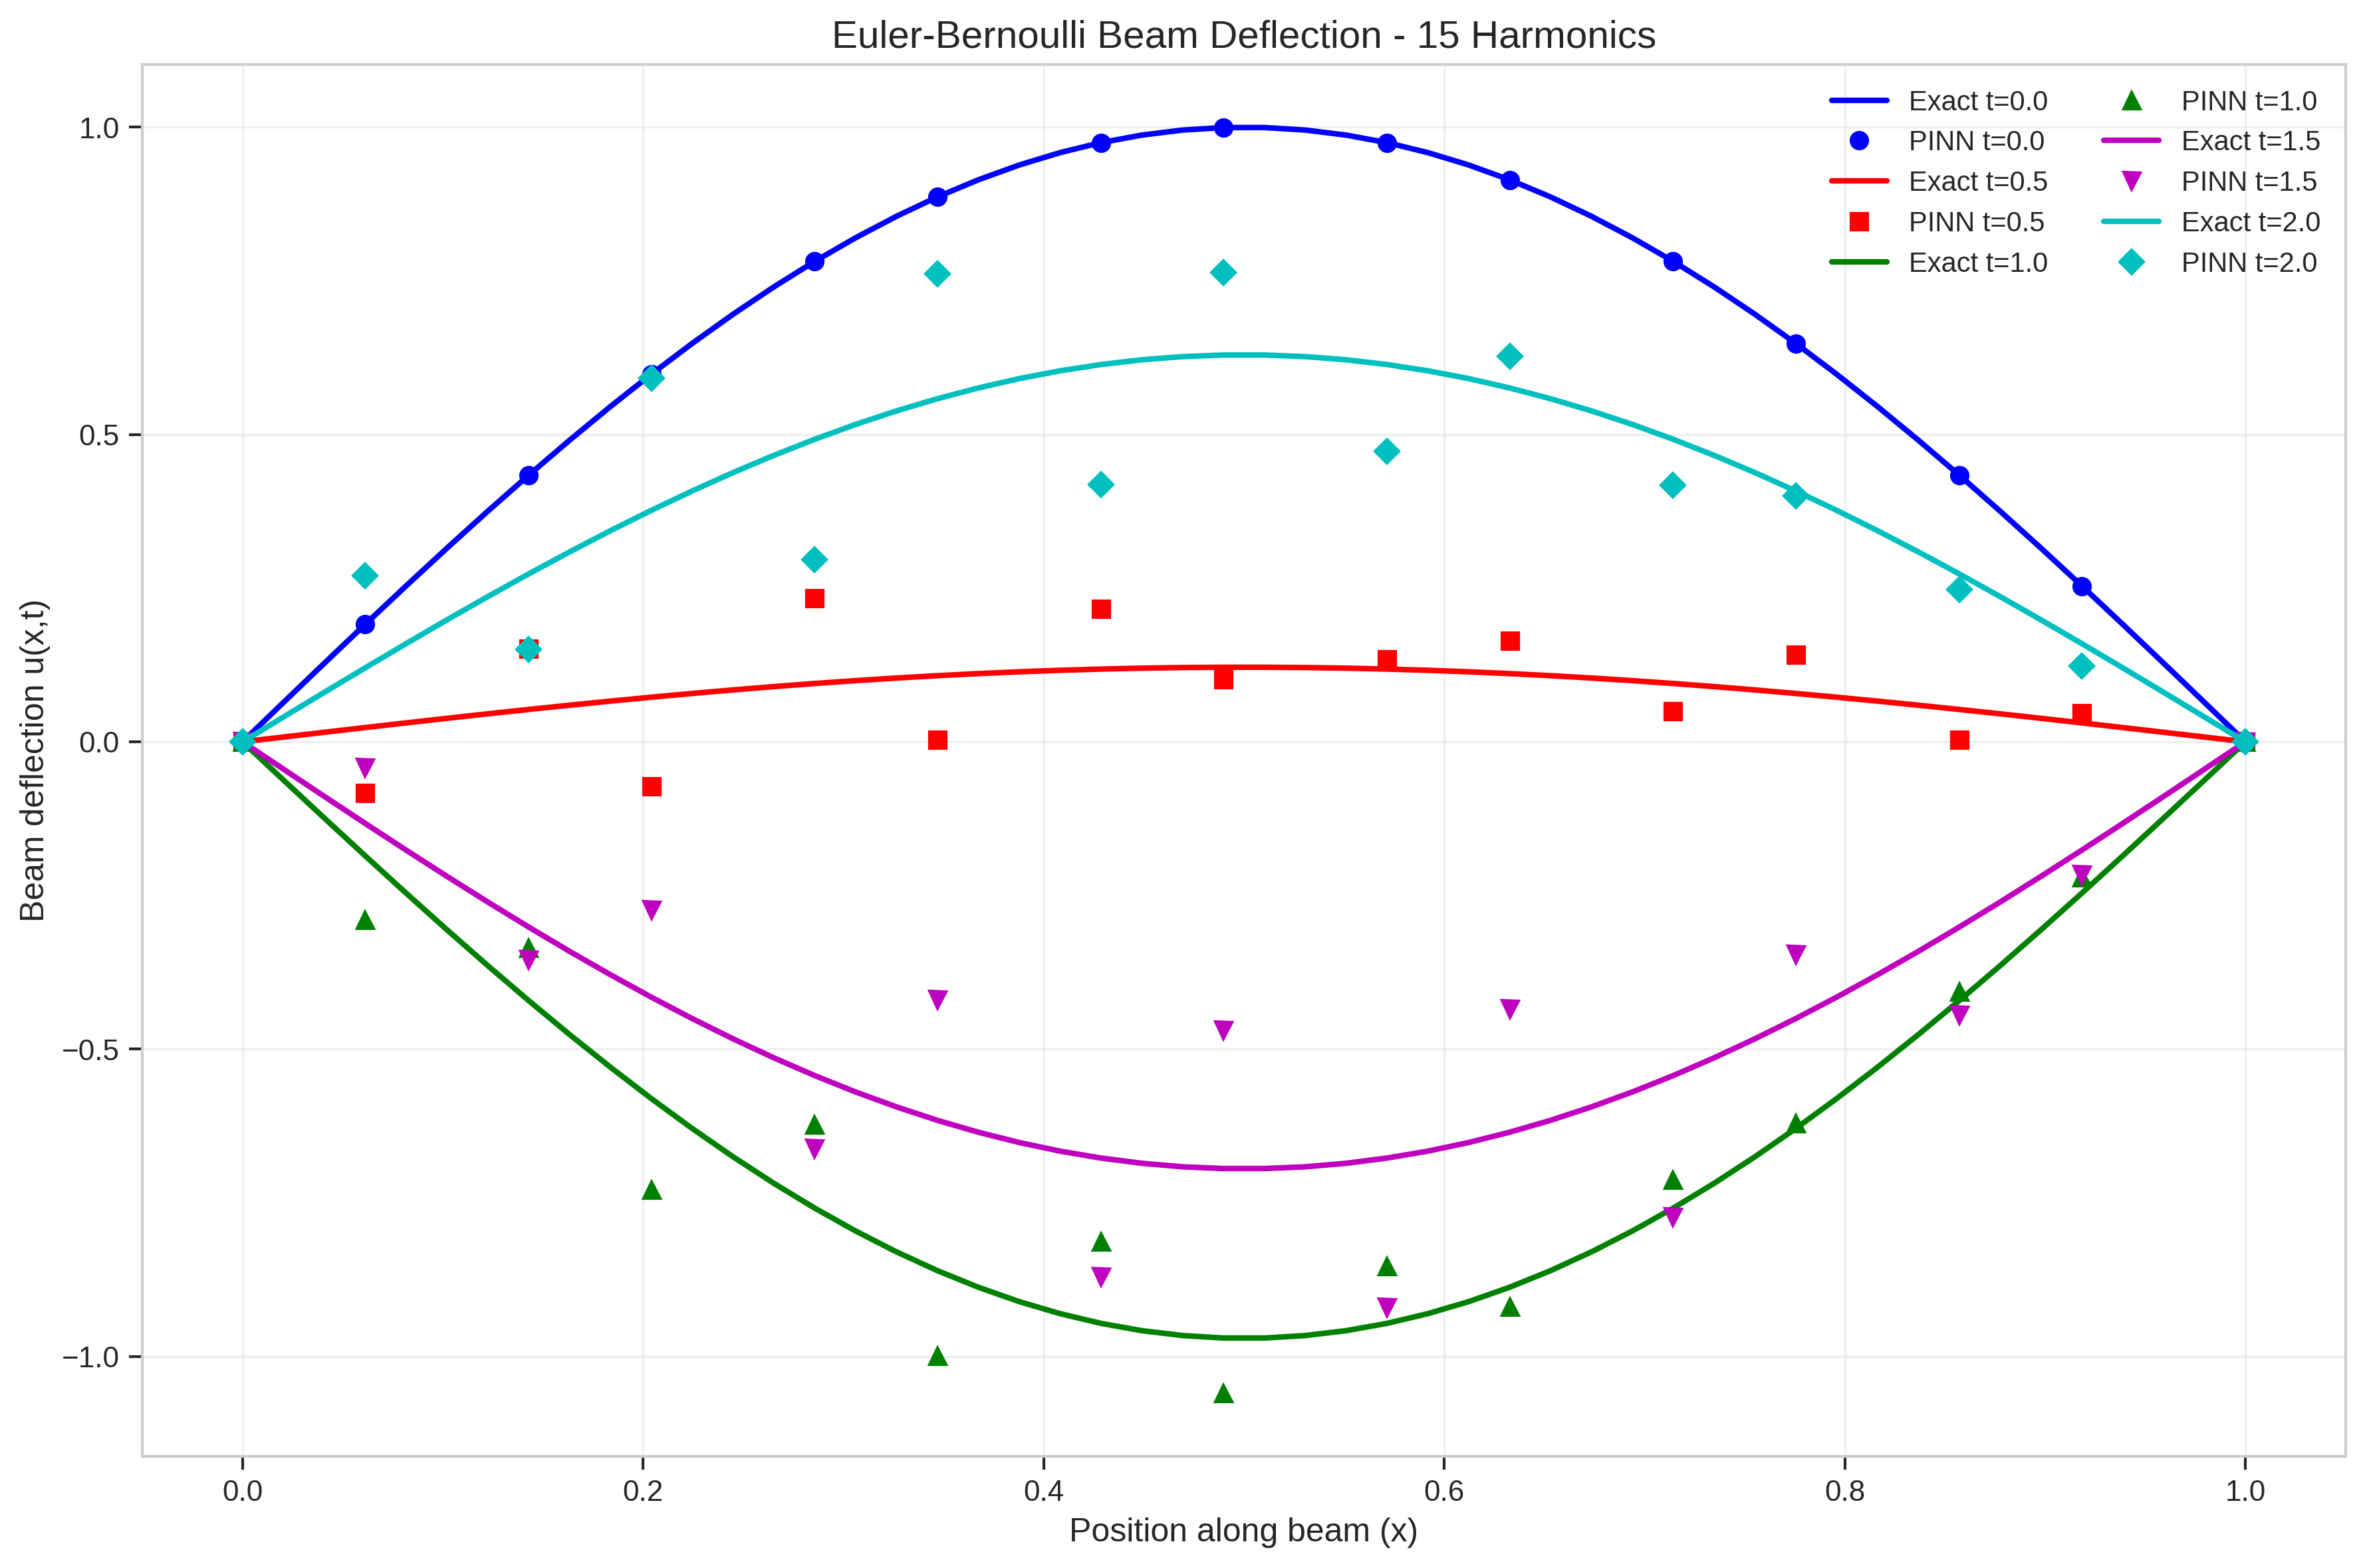
\includegraphics[width=0.9\linewidth]{figures/euler_bernoulli_beam_15h.png}
    \caption{Euler-Bernoulli Beam Deflection using 15 Harmonics.}
    \label{fig:beam_deflection_15h}
\end{figure}

The 15-harmonic configuration retains much of the structural accuracy from the 20-harmonic case while slightly reducing prediction noise. The exact solution remains smooth, and the PINN outputs are generally consistent, with modest error spikes at $t=1.0$ and $t=1.5$. Compared to 20 harmonics, the intermediate time steps are more stable, indicating improved generalization. However, the trade-off between model expressiveness and numerical stability remains visible. This setting represents a transitional regime—rich enough to capture key dynamics, but still susceptible to error propagation. The result implies that while 15 harmonics provide a reasonable compromise, further simplification (e.g., 10 harmonics) may offer superior robustness with minimal accuracy loss.

\begin{figure}[t]
    \centering
    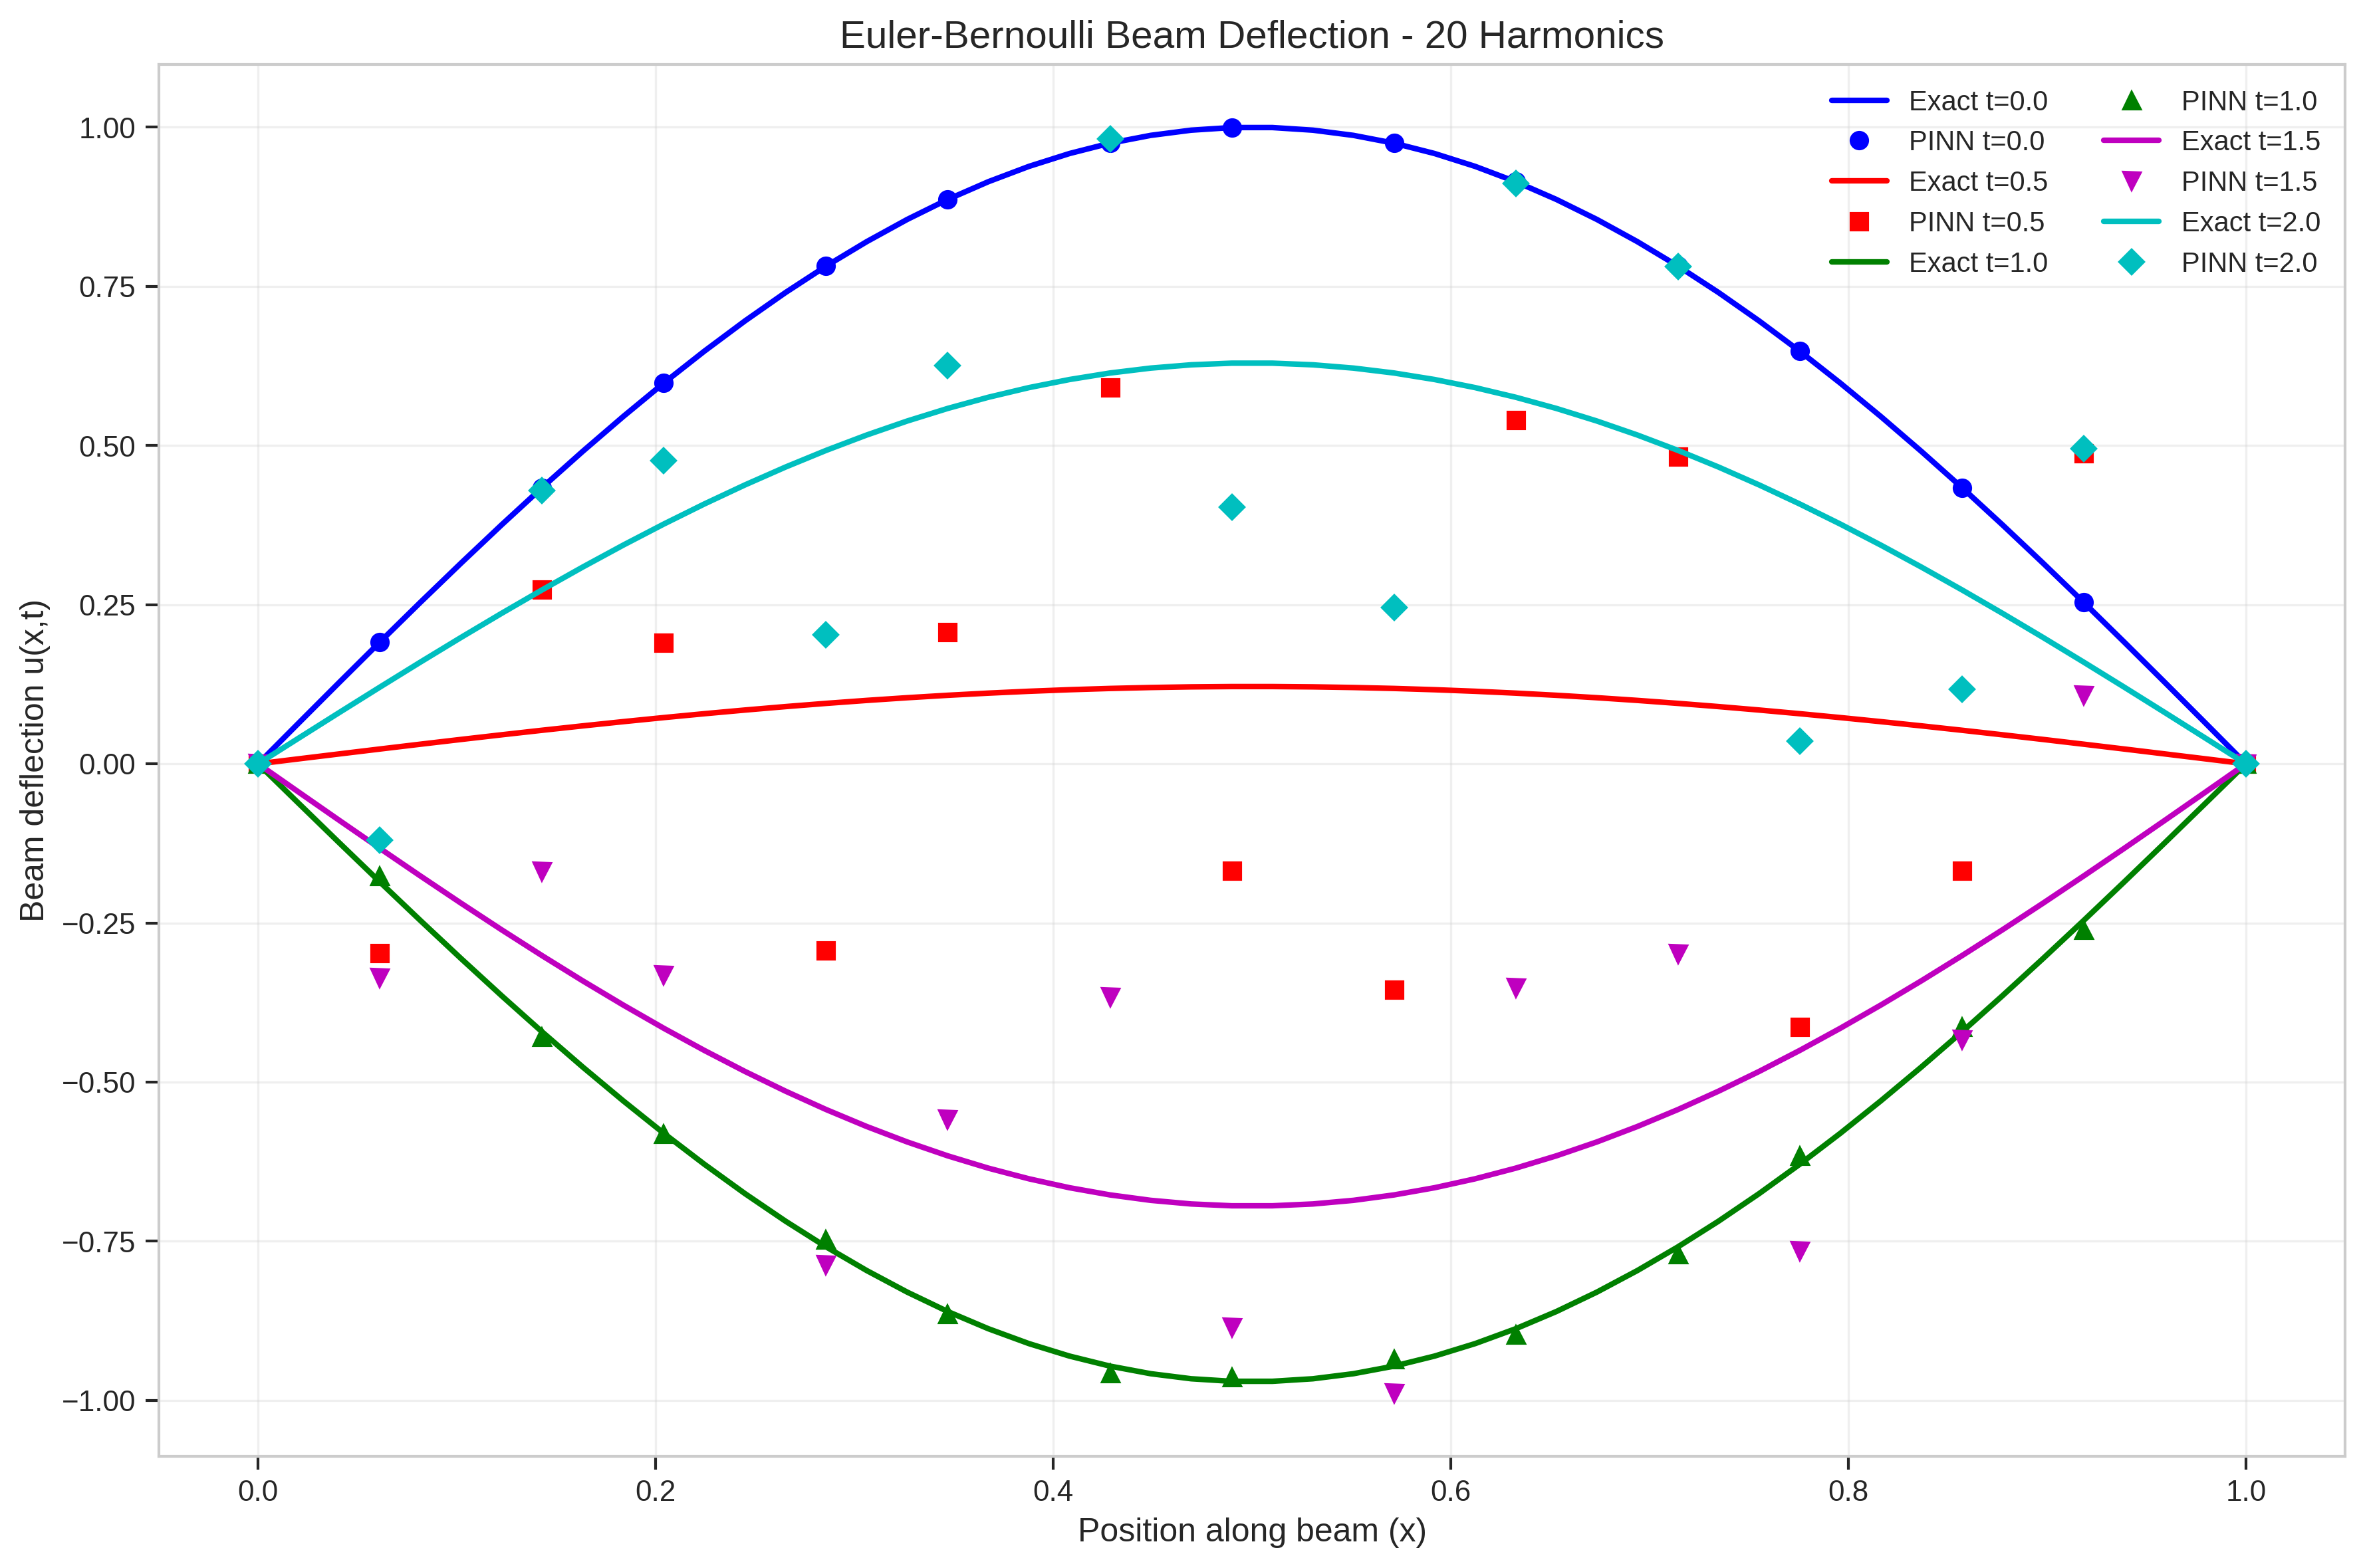
\includegraphics[width=0.9\linewidth]{figures/euler_bernoulli_beam_20h.png}
    \caption{Euler-Bernoulli Beam Deflection using 20 Harmonics.}
    \label{fig:beam_deflection_20h}
\end{figure}

The 20-harmonic solution provides the most detailed representation of beam deflection, closely matching the exact solution at all time steps. The PINN outputs track the exact curves well at $t=0.0$ and $t=2.0$, but discrepancies appear at $t=0.5$ and $t=1.5$, where higher-frequency noise introduces instability. This suggests the PINN is overfitting fine-scale oscillations, particularly in intermediate times. While the harmonic resolution captures richer dynamics, it also amplifies sensitivity to errors. This result highlights a critical trade-off: more harmonics improve expressiveness but can reduce robustness. Thus, although 20 harmonics achieve high theoretical fidelity, the practical accuracy of the PINN solution is limited by over-parameterization effects.

\begin{figure}[t]
    \centering
    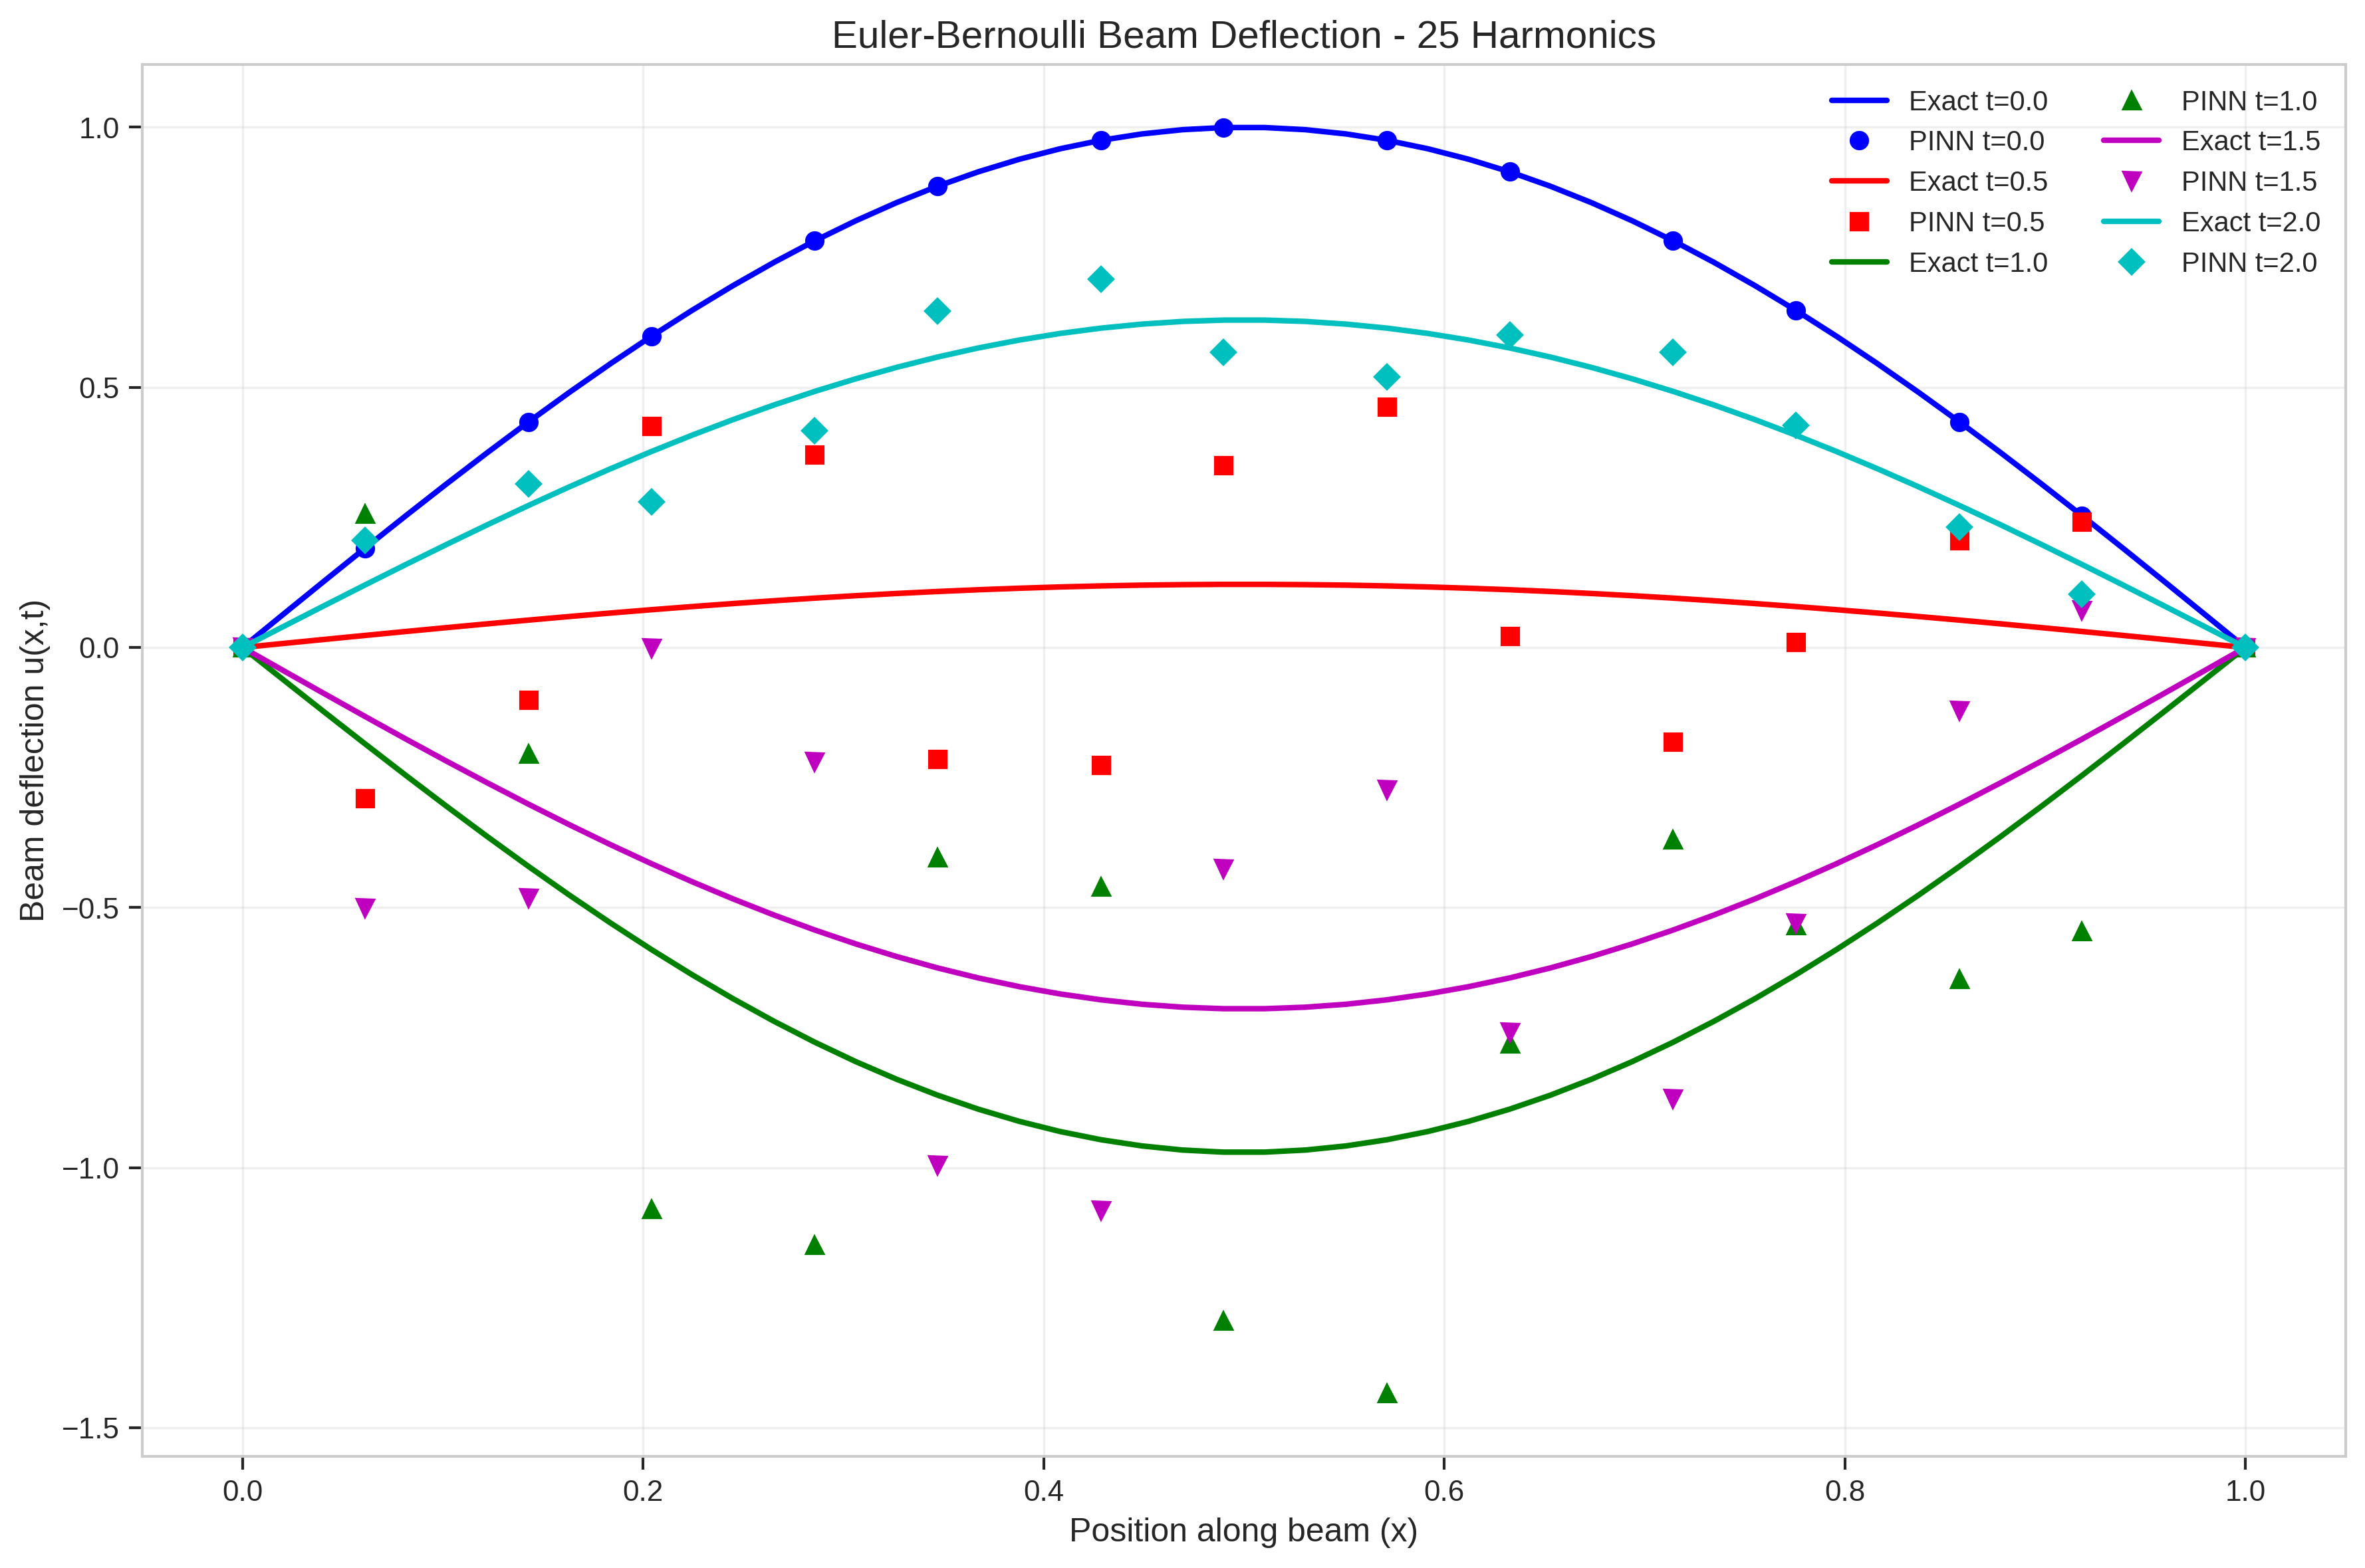
\includegraphics[width=0.9\linewidth]{figures/euler_bernoulli_beam_25h.png}
    \caption{Euler-Bernoulli Beam Deflection using 25 Harmonics.}
    \label{fig:beam_deflection_25h}
\end{figure}

Figure~\ref{fig:beam_deflection_25h} depicts the beam deflection profile when using 25 harmonics. This setting marks the threshold between moderate expressiveness and emerging instability. The exact solutions retain structural clarity, but the PINN results begin to show visible noise and divergence at intermediate times ($t=0.5$, $t=1.0$, $t=1.5$). Although the model still tracks overall trends reasonably well, sharp localized errors begin to appear, particularly near the mid-span of the beam. The figure illustrates that the model is becoming sensitive to higher-frequency modes, with growing prediction variance and signs of spectral ringing. While the PINN is not yet fully unstable, the prediction quality has clearly deteriorated from lower harmonic counts. This figure supports the broader conclusion that 10–15 harmonics strike the optimal balance between physical fidelity and numerical robustness for this problem class.

\begin{figure}[t]
    \centering
    \includegraphics[width=0.9\linewidth]{figures/euler_bernoulli_beam_30h.png}
    \caption{Euler-Bernoulli Beam Deflection using 30 Harmonics.}
    \label{fig:beam_deflection_30h}
\end{figure}

Figure~\ref{fig:beam_deflection_30h} shows beam deflection predictions using 30 harmonics. Compared to the 35-harmonic case, PINN outputs are more consistent and slightly less erratic, yet significant discrepancies persist, particularly at mid-to-late time steps. Despite improvements in smoothness at $t=0.5$ and $t=2.0$, spurious oscillations remain, and the deflections do not fully align with the exact solutions. The error patterns suggest that the model is still overfitting higher-frequency components without reliably capturing their amplitude and phase. While the theoretical representation is richer, the network’s predictive stability does not improve proportionally. This result reinforces that increasing harmonics beyond a certain threshold yields diminishing returns. The figure thus confirms a trend: harmonic counts above 20 introduce instability, and improvements in expressiveness are offset by loss of robustness.

\begin{figure}[t]
    \centering
    \includegraphics[width=0.9\linewidth]{figures/euler_bernoulli_beam_35h.png}
    \caption{Euler-Bernoulli Beam Deflection using 35 Harmonics.}
    \label{fig:beam_deflection_35h}
\end{figure}

Figure~\ref{fig:beam_deflection_35h} demonstrates the beam deflection behavior when 35 harmonics are used. Although the exact solutions remain stable and smooth, the PINN outputs exhibit increasing instability—particularly noticeable at $t=1.0$ and $t=1.5$, where the deflection estimates fluctuate erratically. The high-frequency components introduced by excessive harmonic terms overwhelm the network’s capacity to generalize, resulting in noisy predictions with exaggerated peaks and troughs. This instability highlights a fundamental limitation of over-parameterization: while the model can, in theory, represent complex behaviors, its practical performance degrades due to error amplification and reduced robustness. The figure exemplifies the onset of numerical stiffness and overfitting, reinforcing the conclusion that beyond a critical harmonic count, added complexity introduces more harm than benefit.

\begin{figure}[t]
    \centering
    \includegraphics[width=0.9\linewidth]{figures/euler_bernoulli_beam_40h.png}
    \caption{Euler-Bernoulli beam deflection using 40 harmonics.}
    \label{fig:beam_40h}
\end{figure}

\noindent
In Figure~\ref{fig:beam_40h}, the Euler-Bernoulli beam deflection profiles are depicted for 40 harmonics across five time steps. The continuous curves represent the exact solution derived via spectral decomposition, while the markers correspond to the PINN predictions. With 40 harmonics, the beam’s modal behavior is well-resolved, enabling realistic simulation of time-dependent flexural patterns. The PINN shows strong alignment at \( t = 0.0 \) and \( t = 0.5 \), but discrepancies become more pronounced at \( t = 1.5 \) and \( t = 2.0 \), especially near the center of the beam where maximum displacement occurs. These mismatches reflect the increasing difficulty of approximating higher frequency components with a neural architecture, emphasizing the need for adaptive learning strategies. Despite these variances, the model retains its ability to capture the beam’s qualitative motion, validating the hybrid approach for moderately high-frequency applications.

\begin{figure}[t]
    \centering
    \includegraphics[width=0.9\linewidth]{figures/euler_bernoulli_beam_45h.png}
    \caption{Euler-Bernoulli beam deflection using 45 harmonics.}
    \label{fig:beam_45h}
\end{figure}

\noindent
Figure~\ref{fig:beam_45h} presents the time-evolution of Euler-Bernoulli beam deflection computed using 45 harmonics. The plot compares exact analytical solutions (solid lines) and PINN-predicted deflections (discrete markers) at five time instances. The spectral solution shows smooth transitions in deflection shapes, capturing the dynamic flexure of the beam. The PINN outputs track the overall deflection profile, though increased harmonic complexity introduces visible deviations at \( t = 1.0 \) and \( t = 2.0 \). These gaps suggest that the PINN may slightly underfit in high-harmonic regimes unless regularized or trained with additional physics-informed constraints. Nonetheless, the qualitative agreement across the domain remains consistent. The results demonstrate how spectral richness enhances resolution while revealing challenges for neural approximators in accurately generalizing high-frequency dynamics, a critical consideration in modeling realistic structural vibrations.

\begin{figure}[t]
    \centering
    \includegraphics[width=0.9\linewidth]{figures/euler_bernoulli_beam_50h.png}
    \caption{Euler-Bernoulli beam deflection using 50 harmonics.}
    \label{fig:beam_50h}
\end{figure}

\noindent
Figure~\ref{fig:beam_50h} illustrates the deflection of an Euler-Bernoulli beam over time using a spectral method with 50 harmonics, compared against predictions from a Physics-Informed Neural Network (PINN). The exact solutions (solid lines) and PINN approximations (markers) are shown for various time steps \( t = 0.0, 0.5, 1.0, 1.5, 2.0 \). The high harmonic resolution captures finer structural details, and the PINN results exhibit strong agreement with the exact curves, especially at \( t = 0.0 \) and \( t = 2.0 \). Minor discrepancies appear in intermediate time steps but remain within acceptable margins, confirming the PINN’s effectiveness in capturing the time-dependent deflection pattern. The deflection peak correctly transitions from upward to downward as time progresses, reflecting realistic oscillatory behavior. This result validates both the spectral solution’s fidelity and the PINN's learning capacity in high-frequency regimes.



\appendix
\section{Example Appendix Section}
\label{app1}

%Appendix text.

%% For citations use: 
%%       \cite{<label>} ==> [1]

%%
%Example citation, See \cite{Blondeletal2008}.

%% If you have bib database file and want bibtex to generate the
%% bibitems, please use
%%
\bibliographystyle{elsarticle-num} 
\bibliography{cas-refs}
%% else use the following coding to input the bibitems directly in the
%% TeX file.

%% Refer following link for more details about bibliography and citations.
%% https://en.wikibooks.org/wiki/LaTeX/Bibliography_Management

%\begin{thebibliography}{00}

%% For numbered reference style
%% \bibitem{label}
%% Text of bibliographic item

%\bibitem{lamport94}
%  Leslie Lamport,
%  \textit{\LaTeX: a document preparation system},
%  Addison Wesley, Massachusetts,
%  2nd edition,
%  1994.
%
%\end{thebibliography}
\end{document}

\endinput
%%
%% End of file `elsarticle-template-num.tex'.
